%%
%% Meta: Master Document
%% Arithmetik und Algebra I
%% 
%%

\input{bbwLayoutDoc}

\renewcommand{\author}{Philipp G. Freimann}
\renewcommand{\grafikautor}{Ph. G. Freimann}
\renewcommand{\authoremail}{philipp.freimann@bbw.ch}
\renewcommand{\erstellungsdatum}{\versionTALSMajorDate}
\renewcommand{\docversion}{\versionTALSMajorVSR}

%%\renewcommand{\modulnummer}{Arithmetik und Algebra I}
\renewcommand{\doctitel}{Grundlagenfach Mathematik}
\renewcommand{\fachthema}{4jährige BM1}

%%%%%%%%%%%%%%%%%%%%%%%%%%%%%%%%%%%%%%%%%%%%%%%%%%%%%%%%%%%%%%%%%%%%
%% Gesamt-Skripts benötigen ALINONE (all in one), damit Referenzen auf andere
%% Kapitel funktioniren:
\isALLINONEtrue%%

\scriptStart{}

%% Einstiegsaufgaben
%%
%% 2019 07 04 Ph. G. Freimann
%%

\section*{Einstiegsaufgabe}
\sectuntertitel{Der Anfang ist die Hälfte des Ganzen (Aristoteles)}
%%%%%%%%%%%%%%%%%%%%%%%%%%%%%%%%%%%%%%%%%%%%%%%%%%%%%%%%%%%%%%%%%%%%%%%%%%%%%%%%%
%%Lehrmittel:
%%\GESO{\cite{marthaler21alg} ab. S. 22}
%%\TALS{\cite{frommenwiler17alg} und \cite{frommenwiler18geom}}

\subsection*{Abholen des Bekannten und Geübten}

\TALS{\olatLinkPruefung{Einstiegstest}{https://olat.bbw.ch/auth/RepositoryEntry/572162090/CourseNode/106131924079692}}

\subsubsection*{Die Konservendose}
Stellen Sie sich vor, ein guter Freund von Ihnen stellt Konservendosen her.

Sie müssten für ihn eine optimale Dose in Form eines Kreiszylinders entwerfen, die möglichst wenig
Material benötigt.

\begin{center}
\raisebox{-1cm}{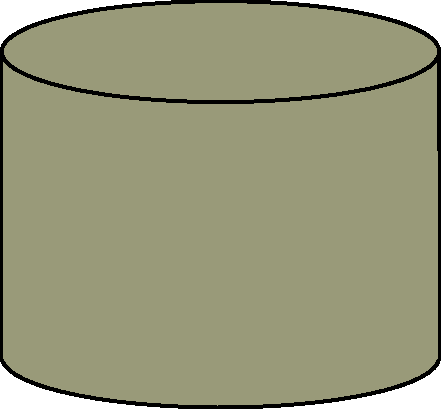
\includegraphics[width=5cm]{tals/010/img/Konservendose.pdf}}
\end{center}

Ihr Freund will exakt einen Liter
Zwiebelsuppe\footnote{S. \textit{Asterix} «Der Kupferkessel»} pro Dose abfüllen.

Wie hoch, wie breit (Radius/Durchmesser) muss die Dose nun sein,
damit \textbf{möglichst wenig Blech} verwendet wird? Was sind Ihre
Überlegungen dazu? Welche Formeln kennen Sie schon? Eine Näherung auf
5\% bis 10\% Genauigkeit sollte schon reichen; eine exakte Berechnung ist hier nicht gefordert.


\newpage
Platz für Ihre Überlegungen:
\TNTeop{
  Volumen = 1 Kubikdezimeter:

  $$r^2\pi \cdot{} h = 1 \text{ dm}^3$$

  $$\Longrightarrow h = \frac1{r^2\pi}$$

  Oberfläche:

  $$O = 2r\pi\cdot{}h + 2r^2\pi = 2r\pi\cdot{} \frac1{r^2\pi} +
  2r^2\pi = \frac2r + 2r^2\pi$$

  Minimieren = Ableitung = 0 setzen

  $$\frac{dO}{dr} = \frac{-2}{r^2} + 4r\pi \stackrel{!}{=} 0$$
  $$\Longrightarrow r^3 = \frac1{2\pi} \Longrightarrow
  r=\sqrt[3\,\,]{\frac1{2\pi}} \approx 0.541926 \Longrightarrow d=h\approx  1.08385 \text{ dm}$$

  Eine Näherung von 1.1 dm sollte hier aber bereits reichen: Eine
  Berechnung oder genauere Annäherung war nicht verlangt.
}



%% Part Arithmetik und Algebra 1
%%%%%%%%%%%%%%%55
%% Funktionen II TALS Metapackage
\part{Funktionen II}\index{Funktionen!II|textbf}
\renewcommand{\bbwPartID}{FCT2}
%%
%% 2019 07 04 Ph. G. Freimann
%%

\section{Quadratische Funktionen}\index{Funktionen!quadratische}
\sectuntertitel{Geraden im Lande der Parabeln wird dringend angeraten, einen
  Integrationskurs zu besuchen.}
%%%%%%%%%%%%%%%%%%%%%%%%%%%%%%%%%%%%%%%%%%%%%%%%%%%%%%%%%%%%%%%%%%%%%%%%%%%%%%%%%

%%\bbwCenterGraphic{8cm}{tals/fct2/img/lugano2018.jpg}
%%\textit{Bildlegende: Parabeln in Lugano (2018)}
\bbwCenterGraphic{175mm}{tals/fct2/img/paris2022.jpg}
\textit{Bildlegende: Parabeln in den Gärten von Versailles (2022)}

\subsection*{Lernziele}

\begin{itemize}
\item Definition
\item Formen: Scheitel-, Produkt-, Normalform
\item Graphische Darstellung
\item Translationen und Spiegelungen
\end{itemize}

\TadBMTA{260}{15}
%%\TALS{(\cite{frommenwiler17alg} S.183 (Kap. 3.4))}
%%\GESO{(\cite{marthaler21alg}       S.260 (Kap. 15))}

Einstieg: Bilder von Heimgartner/Hunziker.


\textbf{Einstiegsaufgabe: } \aufgabenFarbe{Lösen Sie Aufgaben 1. und 2.
  von Seite 272: Welche der angegebenen Funktionen sind quadratisch?}

\newpage

\subsection{Parabel}\index{Parabel}\index{Normalparabel}

Zeichnen Sie die Funktionen $f: y=x^2$ (= Normalparabel), $y=\frac{1}{3}x^2$

und $y=-0.25\cdot{}x^2$  ins Koordinatensystem:

\bbwGraph{-3}{3}{-3}{7}{
  \TRAINER{\bbwFuncC{\x * \x}{-2.5:2.5}{green}
    \bbwFuncC{-0.25*\x * \x}{-3:3}{green}
    \bbwFuncC{\x * \x / 3}{-3:3}{green}
  }
}


\newpage

\subsection{Grundform}\index{Grundform!quadratische Funktion}\index{Quadratische Funktion!Grundform}
Die Funktion $f(x): x \mapsto y = ax^2 + bx +c$ ist eine
quadratische Funktion in Grundform\index{Grundform!quadratische Funktion}.

Spielen Sie mit \TALS{dem TI-nSpire oder mit} \texttt{geogebra.org} an den Parametern $a$, $b$ und $c$ der Funktionsgleichung $y = a\cdot{}x^2 + b\cdot{} x + c$ herum. Was bewirkt der Parameter

$a$: \LoesungsRaumLang{Parabelöffnung: $|a|$ klein: Breite (weite) Öffnung / $|a|$ groß: Enge, schmale Öffnung. $a < 0$: Parabel ist nach unten geöffnet. $a > 0$: Parabel ist nach oben geöffnet.}

$b$: \LoesungsRaumLang{«Parabelsteigung»\footnote{Mit «Parabelsteigung» ist hier die Steigung der entsprechenden Tangente gemeint.} im Punkt $A(0|c)$}

$c$: \LoesungsRaumLang{$y$-Achsenabschnitt. Damit wird eine Verschiebung der Parabel entlang der $y$-Achse erreicht.}

Versuchen Sie eine Parabel mit Scheitelpunkt $(1|1)$ zu finden\TRAINER{(Lösung: $b=-2a$ und $a+b+c=1$.)}.

\subsection*{Aufgaben}
%%\TALSAadBMTA{184ff}{660. a) c) f), 662. a) b) c) und e)}
\AadBMTA{273}{5., 6., 7., 8. und 9.}
\newpage

\subsection{Vier charakteristische Punkte}
Zeichnen Sie die Funktion
$$p: y = x^2 - 4x + \frac{7}{4}$$

\bbwGraph{-3}{6}{-3}{2}{
\TRAINER{\bbwFunc{\x*\x - 4*\x + 1.75}{-0.2:4}}
}%% end BBW Graph

Wo befinden sich die charakteristischen Punkte?

\TNT{2.4}{\vspace{24mm}}


Die charakteristischen Punkte sind:
\begin{itemize}
\item Schnittpunkt mit $y$-Achse = (\LoesungsRaum{0} | \LoesungsRaum{1.75})
\item Nullstellen: $N_1=(\LoesungsRaum{0.5}| \LoesungsRaum{0}), N_2=( \LoesungsRaum{3.5}|\LoesungsRaum{0})$
\item Scheitelpunkt: $S=(\LoesungsRaum{2}|\LoesungsRaum{-2.25})$
\end{itemize}
 
Wie berechnen sich nun diese Punkte?
\newpage
\subsubsection{Parabelöffnung}
Eigentlich ist die Parabelöffnung kein charakteristischer
Punkt. Dennoch kann man eine $x$-Einheit vom Scheitelpunkt entfernt,
das $a$ der Grundform ($y=ax^2+bx+c$) direkt ablesen. Gehen wir bei
der Normalparabel ($a=1$) vom
Scheitelpunkt um eine Einheit nach rechts, so muss die Parabel um eine
$y$-Einheit nach oben anwachsen.

\TNT{10}{
Parabel durch Scheitelpunkt $P=(-3|1)$ und durch $(-2|2)$ =
verschobene Normalparbel zeichnen.

Parabel mit Scheitelpunkt $P=(2|2)$ durch $(3|0.5)$ zeichnen. Das $a$
ist somit sofort $a=-1.5$ abzulesen.
}

\subsubsection{$y$-Achsenabschnitt}
Genau wie bei der linearen Funktion, gilt für den $y$-Achsenabschnitt,
dass die $x$-Koordinate dieses Punktes Null ist.
$$y = x^2 -4x + 1.75$$
wird mit $x=0$ zu
$y = 1.75$.

Der $y$-Achsenabschnitt ist somit immer das $c$ aus $y = ax^2 + bx +
c$.

\newpage

\subsubsection{Nullstellen}
Wie bei den linearen Funktionen sind auch hier die
Nullstellen die Schnittpunkte mit der $x$-Achse. Dies bedeutet für die
Nullstellen $N(x_0 | y_0)$, dass die $y$-Koordinate = 0 ist. Es gilt
also

$$0 = x^2 - 4 x + \frac{7}{4} $$

Dies ist eine quadratische Gleichung mit den Lösungen:

$$x_{1,2} = \frac{-b \pm \sqrt{b^2-4ac}}{2a}$$ 

\noTRAINER{\platzFuerBerechnungen{2.4}}
\TRAINER{$x_{1} = 0.5; x_{2}=3.5$ (Mitternachtsformel)
  \vspace{3cm}}

\begin{bemerkung}{}{}
  Die Nullstellen der quadratischen Funktion entsprechen den Lösungen
  der zugehörigen quadratischen Funktion (mit $y=0$). Daher gilt
  auch hier: 


  \begin{tabular}{c|p{8cm}}
    Diskriminante $D=b^2-4ac$ > 0 & Es gibt zwei Nullstellen. \\
    \hline\\
    Diskriminante $D=b^2-4ac$ = 0 & Es gibt eine Nullstelle, denn der Scheitelpunkt liegt auf der $x$-Achse.\\
    \hline\\
    Diskriminante $D=b^2-4ac$ < 0 & Es gibt keine Nullstellen, denn die Parabel schneidet die $x$-Achse nicht.\\
  \end{tabular}
  
 \ifisALLINONE{Zum Begriff \textbf{Diskriminante}:  \totalref{diskriminante}}\fi{} 
\end{bemerkung}

\subsection*{Aufgaben}
\AadBMTA{277ff}{28. a) c) }

\newpage



\subsubsection{Scheitelpunkt}\index{Scheitelpunkt}
Der Tief- bzw. Hochpunkt einer Parabel wird \textbf{Scheitelpunkt}
genannt.

Wir berechnen den Scheitelpunkt in zwei Schritten.

\textbf{Erstens:} Wir berechnen den Mittelwert der beiden Nullstellen:
$$x_S := \frac{x_{1} + x_{2}}{2} = \frac{\frac{-b+\sqrt{D}}{2a} + \frac{-b-\sqrt{D}}{2a}}{2} =
\frac{(-b+\sqrt{D}) + (-b-\sqrt{D})}{4a} =\frac{-b}{2a}$$
Dabei ist $D$ die Diskriminante $D=b^2-4ac$.

\platzFuerBerechnungen{2.4}
\TRAINER{$x_S = 2$
\vspace{3cm}}

\textbf{Zweitens:} Wir setzen den gefundenen $x$-Wert
(\LoesungsRaum{2}) in die Funktionsgleichung
ein:
$$y_S = x^2 - 4x + 1.75$$
$$y_S = (\LoesungsRaum{2})^2 - 4\cdot{}(\LoesungsRaum{2}) + 1.75$$

Wir erhalten für den Scheitelpunkt $S$: $S=(x_S | y_S) = (\LoesungsRaum{2} | \LoesungsRaum{-2.25})$.

\begin{gesetz}{Scheitelpunkt}{}
  Der Scheitelpunkt $S$ einer Parabel in der Grundform ($y=ax^2+bx+c$) kann wie folgt
  berechnet werden:

  $$S=\left(\frac{-b}{2a}\middle|\frac{4ac-b^2}{4a}\right)$$

  (Bem.: Der $y$-Wert kann einfach durch Einsetzen des $x$-Wertes in
  die Funktionsgleichnug gefunden werden.)
  \end{gesetz}
  
\subsection*{Aufgaben}
%%\TALSAadBMTA{184ff}{665. a) b) c) 666. a) b) c) e) f) g)}
\AadBMTA{273}{4. (=Aufg. 22. S. 276)}

\newpage

\subsection{Bestimmen der Funktionsgleichung}
\TALS{S. 187 Kap. 3.4.3}

\subsubsection{Referenzaufgaben}

\textbf{TYP I}

Gegeben ist ein Punkt $P$ mit den Koordinaten $(2.3 | -1.5)$. Gesucht ist die reinquadratische Funktion $f: y=a\cdot{}x^2$, welche durch diesen Punkt geht.
Machen Sie vorab eine Skizze.

\bbwGraph{-3}{3}{-2}{1}{
  \TRAINER{\bbwFunc{-0.2836 * \x * \x}{-2.5:2.5}
    \bbwDot{2.3,-1.5}{blue}{west}{P}
  }%% end TRAINER
}%% end BBW Graph

\platzFuerBerechnungen{3.6}

\TRAINER{Idee: Punkt einsetzen: $-1.5 = a\cdot{}(2.3)^2$. Das Auf"|lösen dieser Gleichung liefert $a = \frac{-1.5}{2.3^2}$. Dies liefert $a\approx -0.2836$}

Weitere «TYP 1» Aufgaben wären z. B. $y = 3x^2 - bx + 4$ oder $y=2x^2
-7x + c$ mit anderen Worten alle Parabeln mit genau \textbf{einem}
Parameter, daher «Typ 1».

\newpage



\textbf{TYP II}

Gegeben sind zwei Punkte und wir haben zwei Unbekannte.

\begin{rezept}{}{}
  Gesucht sind $a$ und $c$ aus $y = ax^2 + c$ bei den gegebenen
  Punkten $(7|5)$ und $(2|-4)$.

  Wir lösen dies auch durch Einsetzen der Punkte in die
  Funktionsgleichung und wir erhalten zwei Gleichungen:


  \begin{tabular}{c | r  c  r |}
    (I)  &  $5$ & = & $(7)^2\cdot{} a + c$ \\
    (II) & $-4$ & = &  $(2)^2\cdot{} a + c$ \\
  \end{tabular}

  Durch Subtrahieren der Gleichungen erhalten wir

  \begin{tabular}{c | r  c  r | c}
    (I)  &  $5$ & = & $49\cdot{} a + c$ & \,\\
    (II) & $-4$ & = &  $4\cdot{} a + c$ & $\ominus$\\
  \end{tabular}

  $$9 = 45a$$ und somit
  $$a =\frac{1}{5}.$$

  Dieses $a$ (= $\frac{1}{5}$) setzen wir nun in eine der Gleichungen
  (\zB (I)) ein und erhalten
  $$5=49\cdot{}\frac{1}{5} + c$$
  und nach Auf"|lösen erhalten wir $c=\frac{-24}{5}$.

  Die gesuchte Gleichung lautet also:

  $$y = \frac{1}{5}x^2 - \frac{24}{5}$$
\end{rezept}

Probe durch Einsetzen der $x$-Werte der Punkte in die gefundene Funktionsgleichung:

\TNTeop{}
%%\newpage

\begin{beispiel}{}{}
  Anstelle von $a$ und $c$ können natürlich auch $a$ und $b$ gesucht
  sein. Daher eine zweite Aufgabe.

  Gesucht sind $a$ und $b$ aus $y = ax^2 + bx$ bei den gegebenen

  Punkten $(2|-6)$ und $(-3|5)$.

  Wir lösen dies wiederum durch Einsetzen der Punkte in die
  Funktionsgleichung und wir erhalten die beiden Gleichungen, welche
  wir durch das Additionsverfahren lösen können:

  \begin{tabular}{c | r  c  r | c}
    (I)  &  $-6$ & = & $4a + 2b$ & $\cdot{} 3$ \\
    (II) &   $5$ & = & $9a - 3b$ & $\cdot{} 2$ \\
  \end{tabular}

  somit:
  
  \begin{tabular}{c | r  c  r | c}
    (I')  & $-18$ & = & $12a + 6b$ &\, \\
     \,   & \,    & \,&   \,       & $\oplus$\\
    (II') &  $10$ & = & $18a - 6b$ &\, \\
  \end{tabular}

  Nach Addition der Gleichungen erhalten wir

  $$-8 = 30a$$

  was uns zu $a=\frac{-4}{15}$ bringt.

Dieses $a$ können wir nun wieder in eine der beiden Gleichungen
einsetzen (\zB in (I)):

$$-6=4\cdot{}\frac{-4}{15} + 2b$$

Das Auf"|lösen obiger Gleichung liefert nach Kürzen: $b=\frac{-37}{15}$.

Die gesuchte Funktionsgleichung lautet also

$$y = \frac{-4}{15} x^2 - \frac{37}{15} x.$$

\end{beispiel}

Auch bei «Typ II» kann natürlich jede \textbf{zwei}parametrige quadratische
Funktion herhalten, wie \zB $y=-6cx^2 + bx - c$ durch \textbf{zwei}
gegebene Punkte.
\newpage


\textbf{TYP III}: Gegeben sind hier drei Punkte, wir haben aber auch
drei Unbekannte in $y = ax^2 + bx + c$. Die Punkte sind hier
(1|3), (2|3.5) und (-3|11).

Durch Einsetzen der drei Punkte je in die Funktionsgleichung erhalten
wir drei Gleichungen:

\begin{tabular}{c|r c rcrcr|}
  (I)   & 3   & = & $(1)^2\cdot{}a$  &$+$& $(1)\cdot{}b$  &$+$& c \\ 
  (II)  & 3.5 & = & $(2)^2\cdot{}a$  &$+$& $(2)\cdot{}b$  &$+$& c \\ 
  (III) & 11  & = & $(-3)^2\cdot{}a$ &$+$& $(-3)\cdot{}b$ &$+$& c \\ 
\end{tabular}

Vereinfachen:

\begin{tabular}{c|r c rcrcr|}
  (I)   & 3   & = & $a$  &$+$& $b$  &$+$& c \\ 
  (II)  & 3.5 & = & $4a$ &$+$& $2b$ &$+$& c \\ 
  (III) & 11  & = & $9a$ &$-$& $3b$ &$+$& c \\ 
\end{tabular}

Nun finden wir $a$, indem wir zunächst $c$ durch Subtraktion
eliminieren:

\begin{tabular}{l|r c rcr|}
  (IV) = (II) -   (I) & 0.5  & = & $3a$ &$+$& $b$ \\ 
  (V)  = (III) - (II) & 7.5  & = & $5a$ &$-$& $5b$ \\ 
\end{tabular}

Multiplizieren wir nun die Gleichung (IV) mit 5, so erhalten wir

\begin{tabular}{r|r c rcr|}
  5$\cdot{}$(IV)  & 2.5  & = & $15a$ &$+$& $5b$ \\ 
  (V)             & 7.5  & = & $5a$  &$-$& $5b$ \\ 
\end{tabular}

Durch Addition der beiden Gleichungen (IV) und (V) erhalten wir

$10 = 20a$ oder $a = \frac{1}{2}$.

Um $b$ zu finden, setzen wir $a = \frac{1}{2}$ in (V) ein: $7.5 =
5\cdot{}\frac{1}{2} - 5b$.

Auf"|lösen nach $b$ ergibt $b = -1$.

Zu guter Letzt setzen wir $a = \frac{1}{2}$ und $b=-1$ in die
Gleichung (I) ein, um noch $c$ zu erhalten:

$$3 = a + b + c = \frac{1}{2} - 1 + c$$

Somit ist $c=3.5$ und die Funktionsgleichung lautet:

$$y = \frac{1}{2}x^2 - x + 3.5$$


\TALS{\subsection*{Aufgaben}}
%%\TALSAadBMTA{187ff}{676. a) c), 682., 684.}
\AadBMTA{272}{3. a) c), 20. a) c), 21., 22., 24. a), 25. b)}
\newpage


\subsection{Computer Algebra Systeme (CAS)}\index{CAS}
Das eben gezeigte Beispiel wird in der Praxis meist nicht von Hand,
sondern mit einem Computer-Algebra-System, kurz CAS, gelöst:

\paragraph{Aufgabenstellung}
Gegeben sind wieder drei Punkte (1|3), (2|3.5) und (-3|11).
Gesucht ist die Parabel $y = ax^2 + bx + c$, welche durch die drei
Punkte geht.

Dies wird mit dem \tinspire{} wie folgt gelöst:
\begin{itemize}
\item Definiere die Funktionsgleichung mit
  Parametern\footnote{\tinspire Regel: $ax\ne a\cdot{} x$}:\\
  $$f(x) := a\cdot{}x^2 + b\cdot{}x + c$$
\item Definiere das Gleichungssystem:
  $$gls := \left\{ \begin{array}{l}
    f(1) = 3\\
    f(2) = 3.5\\
    f(-3)= 11\\
  \end{array}\right.$$
\item Löse das Gleichungssystem:
  $$solve(gls,\{a, b, c\})$$
\end{itemize}

\subsection*{Aufgaben}
\AadBMTA{272}{3. b) d)}

\newpage

\subsection{Formen der quadratischen Funktion}
\subsubsection{Nullstellenform}\index{Nullstellenform}

Die \textbf{Nullstellenform} wird auch  «faktorisierte Form» oder
«Produktform» genannt.\index{faktorisierte Form}\index{Produktform}

Beachten Sie die folgende quadr. Funktionsgleichung:

$$y = 3.1(x-5)(x+6)$$

Dies ist eine quadratische Funktion in der sogenannten
\textbf{Nullstellenform}, denn die Nullstellen (hier $x_0 = 5$ oder
$x_0 = -6$) können direkt aus der Funktionsgleichung abgelesen werden.
Wenn wir $y=0$ in die Gleichung setzen (Nullstelle),

$$0 = 3.1(x-5)(x+6)$$
so wird die Gleichung genau dann wahr, wenn (mind.) einer der beiden Klammerausdrücke rechts
gleich Null ist. Die Parabelöffnung (hier 3.1) kann dabei beliebig variieren und ist (neben den Nullstellen) der einzige Parameter.

Die Nullstellenform lautet

\begin{gesetz}{}{}

  $$y = a(x-x_1)\cdot{}(x-x_2)$$

  \end{gesetz}

wobei $x_1$ und $x_2$ die Nullstellen der Parabel bezeichnen. 
\newpage


\subsubsection*{Referenzaufgabe zur Nullstellenform}

\noTRAINER{\bbwGraphic{16cm}{tals/fct2/img/BrunnenNullstellenformOhneKoordinatensystem.png}}
\TRAINER{\bbwGraphic{16cm}{tals/fct2/img/BrunnenNullstellenformMitKoordinatensystem.png}}

Ein parabelförmiger Wasserstrahl spritzt ebenerdig aus einem Brunnen und trifft 7m von der Düse entfernt wieder auf dem Boden auf.
Das Wasser steigt also erst gleich hoch an, wie es danach wieder «herunterfällt».
Dabei wird gemessen, dass 1m von der Düse entfernt der Wasserstrahl 84cm über Boden verläuft.
Können Sie aufrecht unter dem Wasserstrahl hindurchgehen?

Tipp: Skizze und  die Parabelgleichung in Nullstellenform aufschreiben. Die Düse ist der Ursprung der Koordinatensystems.\\

\TNT{5.2}{Die Funktionsgleichung lautet $y=a(x-x_1)(x-x2)$.\\
  Mit den Nullstellen $x_1=0$ und $x_2=7$.\\
  Wir setzen den gemessenen Punkt (1|0.84) in die Gleichung ein und erhalten $0.84 = a\cdot{}(1-0)(1-7)$.\\
  Daraus ergibt sich $a=0.84/(-6) = -0.14 $.\\
  Nun setzen wir 3.5 Meter in die Funktionsgleichung $y = -0.14(x-0)(x-7)$ ein: und erhalten $y=-01.4\cdot{}3.5\cdot{}(-3.5) = 1.715m$; das ist die höchste Parabelstelle.}


\subsection*{Aufgaben}%% Nullstellenform
%%\TALSAadBMTA{185}{663, 678., 680.}
\TALSAadBMTA{277}{30. a) b), 31. b)}
\newpage

%%\TRAINER{\, \newpage}
\subsubsection{Scheitelform}\index{Scheitelform!der quadratischen
  Funktion}
Einstieg: Wo hat die Parabel $f: y=3.6(x-4)^2 + 5$ ihren
Scheitelpunkt?

\TNT{4.4}{CAS: bei $x_S = 4$ und $y_S= 5$; völlig irrelevant ist die 3.6.}

Ist eine quadratische Funktion in der Form
\begin{gesetz}{}{}
$$y = a(x-x_S)^2 + y_S$$
\end{gesetz}
gegeben, so sprechen wir von der \textbf{Scheitelform} oder Scheitelpunktsform.
Das liegt daran, dass diese Parabel ihren Scheitelpunkt bei
$(x_S|y_S)$ hat.

Setzen wir für $x$ = $x_S$ in die Funktionsgleichung, so erhalten wir
gerade die $y$-Koordinate des Scheitelpunktes. Je weiter wir uns nun
mit $x$ von $x_S$ wegbewegen, umso größer wird der Term $(x-x_S)^2$
und zwar in egal welcher Richtung wir uns von $x_S$ wegbewegen, die
$y$-Koordinate verhält sich in beiden Fällen symmetrisch.

Prüfen Sie dies mit TI-nSpire oder \texttt{geogebra.org} an der Funktion

$$y = a\cdot{}(x-p)^2 + q$$

Definieren Sie dabei auch den Punkt $S=(p|q)$. Spielen Sie nun mit
$a$, $p$ und $q$. Was bewirken die Änderungen?
\newpage


\subsubsection{Referenzaufgabe Scheitelform}
Von einer Parabel ist der Scheitel $S(2|3)$ gegeben. Ebenfalls ist bekannt, dass die Parabel durch den Punkt $P\left(-\frac{1}{2}\middle|1\right)$ geht.

  Berechnen Sie die Funktionsgleichung in der Grundform $y = ax^2 + bx + c$. Tipp:
  Schreiben Sie die Funktionsgleichung in der Form $y=a(x - x_S)^2 +  y_S$ und setzen anschließend den Punkt $P$ ein.

  \platzFuerBerechnungen{8.0}%%
  \TRAINER{
    Ansatz:
    $$y = a(x-2)^2 + 3$$
    Jetzt $P$ einsetzen:
    $$1 = a(-\frac{1}{2} - 2)^2 + 3 $$
    Nach $a$ auf"|lösen ergibt:
    $$a=-0.32 (=\frac{-2}{2.5^2})$$
    Nun setzen wir $a=-0.32$ in die Funktionsgleichung $y=a(x-2)^2+3$
    ein:
    $$y=-0.32(x-2)^2+3$$
    und quadrieren das Binom, um die geforderte Grundform zu erhalten:
    $$y = -0.32(x^2 - 4x + 4) + 3 = -0.32x^2 + 1.28x + 1.72$$
  }%%end TRAINER%%

  \subsection*{Aufgabe}
  \AadBMTA{277}{29. a) c) e), 32. a), 33.}
%%  \TALSAadBMTA{185}{679. a), 681., 695., 684. a), 700., 694., 686.(*) und  664.}}

\newpage


\subsection{Umrechnungen der Formen}\index{Formen!der quadratischen Funktion}\index{Quadratische Funktion!Formen}

Nochmals die drei Formen im Überblick:


\begin{tabular}{c|l}
  Form & Funktionsgleichung\\
  \hline\\
  Normalform/Grundform & $f: y= ax^2 + bx + c$\\
  \hline\\
  Nullstellenform, faktorisierte Form oder Produktform & $f: y=a(x-x_0)(x-x_1)$\\
  \hline\\
  Scheitelform & $f: y=a(x-x_S)^2+y_S$\\
  \hline%%
\end{tabular}


\subsubsection{Umrechnungen zwischen den Formen}\index{Umrechnungen!quadratische Funktion}\index{Quadratische Funktion!Umrechnungen}

\begin{center}
  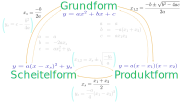
\includegraphics[width=15cm]{allg/funktionen/img/formen/formen.png}
\end{center}

\begin{bemerkung}{}{}
  Das $a$,  ist in allen Formen derselbe Wert und bestimmt die Parabelöffnung.
  \end{bemerkung}
\newpage

\textbf{Grundform aus Scheitelform} (einfaches Ausmultiplizieren). Beispiel:
$$y=2(x-3)^2-4 = 2(x^2-6x+9)-4=2x^2-12x+14$$

\begin{tabular}{rcl}
$a(x-x_S)^2+y_S$ &=& $ax^2-2ax_Sx + (ax_S^2+y_S)$\\
  $a$ &=& $a$ \\
  $b$ &=& $-2ax_S$\\
  $c$ &=& $ax_S^2+y_S$
\end{tabular}


\textbf{Grundform aus Produktform} (einfaches Ausmultiplizieren). Beispiel
$$y=2(x+3)(x-4)=2(x^2 +(3-4)x - 12) = 2x^2-x-24$$

\begin{tabular}{rcl}
  $a(x-x_1)(x-x_2)$ &=& $ax^2 - a(x_1+x_2)x + ax_1x_2$\\
  $a$ &=& $a$ \\
  $b$ &=& $-a(x_1+x_2)$\\
  $c$ &=& $ax_1x_2$
\end{tabular}


\textbf{Nullstellenform (Produktform) aus Grundform}:
Gegeben: $y = ax^2 + bx + c$

Nullstellenform: $y = a(x-x_1)\cdot{}(x-x_2)$ mit

$$x_{1,2} = \frac{-b \pm \sqrt{b^2-4ac}}{2a}$$

\begin{beispiel}{}{}
Gegeben $y = 5x^2 - 5x - 30$. Schreiben Sie dies in der Produktform (=
Nullstellenform):
\platzFuerBerechnungen{3.2}\TRAINER{$y = 5(x-3)(x+2)$\vspace{4.2cm}}
\end{beispiel}
\newpage


\textbf{Scheitelform aus Grundform}:
$$x_S=\frac{-b}{2a}$$

$y_S$ einfach durch Einsetzen von $x_S$ in die Grundform:
$$y_S=c-\frac{b^2}{4a}$$
 
\textbf{Scheitelform aus Produktform}: $x_S$ ist der Mittelwert der beiden
Nullstellen:
$$x_S=\frac{x_1+x_2}{2}$$
Danach $y_S$ einfach durch Einsetzen von $x_S$ in die Produktform:
$$y_S=\frac{-a}{4}(x_1-x_2)^2$$

\textbf{Produktform aus Scheitelform}: Einfachster Weg geht über die Grundform oder abgekürzt:
$$x_{1,2} =x_S \pm \sqrt{\frac{-y_S}{a}}$$


\subsection{Aufgaben}

\TALS{\olatLinkArbeitsblatt{Umrechnen der Formen}{https://olat.bbw.ch/auth/RepositoryEntry/572162090/CourseNode/103176133021102}{1., 2., 3. und 8.}}



\newpage

% Bereits in typ I II und III eingebaut
%\subsection{Parabel aus drei Punkten}
Vorzeigeaufgabe Marthaler Algebra S. 272 Aufg. 3. b) 


\subsection*{Aufgaben}

\AadBMTA{272}{3. a) c)}%% war Marthaler S. 187 Aufg. 676 a) und b)
\GESOAadBMTA{???}{???}

\newpage



%\newpage

%

%%%%%%%%%%%%%%%%%%%%%%%%%%%%%%%%%%%%%%%%%%%%%%%%%%%%%%%%%%%%%%%%
\subsection{Extremwertaufgaben}



\subsubsection{Aus alter Maturprüfung}

\aufgabenFarbe{Gegeben ist die Funktion $f(x) = x\cdot{}(3-\sqrt{x})$,
  $x\in[0;\infty[$.\\
  a) Bestimmen Sie die Nullstellen und das  Extremum der Funktion
  $f$.\\
  b) Im ersten Quadranten, zwischen dem  Graphen und der
  $x$-Achse ist ein  rechtwinkliges Dreieck $ABC$ einbeschrieben.  Der
  rechte Winkel ist in der Ecke $B$.  Punkt $A$ liegt im Ursprung, $B$
  auf der  $x$-Achse und $C$ auf dem Graphen von $f$. Berechnen Sie
  die Koordinaten des  Punktes $C$ so, dass der Flächeninhalt des
  Dreiecks maximal wird.
}%% END aufgabenFarbe

    
\bbwCenterGraphic{8cm}{tals/fct3/img/Maximieren.png}
\TNTeop{
   a) solve$(f(x)=0,x)$ Somit sind die Nullstellen bei 0 und 9\\
     $\text{fmax}(f(x),x)$ liefert $x=4$ ist Maximalstelle (und auch
     Maximalwert ($f(4)=4$)\\
   b) $\text{fmax}(0.5\cdot{}x\cdot{}f(x), x)$ liefert $x = 5.76$ und
   $f(5.76) = 3.456$}%% End TNTeop
\newpage
\subsection*{Aufgaben}
\AadBMTA{311}{49.}
\AadBMTA{321}{17.}

%\newpage

\section{Berührende Graphen}\index{Graphen!berührende}\index{berührende Graphen}

\textbf{Einführungsbeispiel}


Gegeben ist die Parabel $f: y=\frac{1}{4}x^2 -\frac12x +\frac14$ und von einer
Geraden $g$ ist der $y$-Achsenabschnitt $b = -2$ gegeben.

Gesucht ist von der Geraden $g$ die Steigung $a$ so, dass die
Gerade die Parabel tangiert; also genau in einem Punkt berührt.

Wo (in welchem Punkt $B=(x_B|y_B)$) tangiert also die Gerade $g$ die Parabel $f$?

In der folgenden Skizze sind drei mögliche Geraden mit $y$-Achsenabschnitt
$-2$ gezeichnet. Nur eine dieser drei Geraden \textit{tangiert} die Parabel.

\bbwGraph{-4}{4}{-3}{5}{
  \draw[thick,color=blue,variable=\x,domain=-3.5:4] plot ({\x},   {0.25*\x*\x -0.5*\x + 0.25});

  \draw[color=red,variable=\x,domain=-3:5] plot ({\x},{2*\x -2});
  \draw[color=red,variable=\x,domain=-3:5] plot ({\x},{0.5*\x - 2});
  \draw[color=cyan,thick,variable=\x,domain=-3:5] plot ({\x},{1*\x  -2});

  \bbwDot{3, 1}{green}{north}{B}

  %%%\draw[thick,color=blue,variable=\x,domain=-1:5] plot ({\x}, {0.5*\x*\x - 2*\x + 3}); 
  %%\draw[color=red,variable=\x,domain=-1:5] plot ({\x},{0.5*\x + 1});
  %%\draw[color=red,variable=\x,domain=-1:5] plot ({\x},{0.5*\x - 1.5});
  %%\draw[color=cyan,thick,variable=\x,domain=-1:6] plot ({\x},{0.5*\x  -0.125});
  %%\bbwDot{2.5, 1.125}{green}{north}{P}
}
\newpage
\textbf{Lösungsidee}: Der gesuchte Parameter ist $a$, die Steigung der
Geraden.

Nun berechne die Schnittpunkte/den Schnittpunkt mit $$f(x) = g(x).$$

Das $a$ ist gefunden, sobald die Gleichung $f(x)=g(x)$ genau eine
Lösung aufweist; dann also, wenn


\TNT{2}{die Diskriminante dieser Gleichung
verschwindet.}

Den $x$-Wert dieses Berührungspunktes nennen wir $x_B$:


Ansatz:

$$f(x_B) = g(x_B)$$

\TNT{4.4}{
 
\begin{tabular}{rclr}
$\frac14x_s^2-\frac12x_s+\frac14$          & $=$ &  $ax_s-2$ & \\
$\frac14x_s^2+(-\frac12-a)x_s + \frac94$   & $=$ & $0$       & (I)\\
\end{tabular}
\vspace{10mm}
}%% END TNT

Die Diskriminante $D=B^2 - 4AC$ muss gleich 0 sein. 

\TNT{7.2}{
$A = \frac14$, $B = -\frac12-a$ und $C = \frac94$.

  $$D=0=B^2-4AC = (-\frac12-a)^2  - (4\cdot{}A\cdot{}C)$$
  $$0 = (a^2+a+\frac14) - (4\cdot\frac14\cdot{}\frac{+9}4)$$
$$\Longrightarrow 0 = a^2 + a - 2$$
$$\Longrightarrow a_1 = 1 \text{ und  } a_2 = -2$$
\vspace{40mm}
}%% END TNT
\newpage

Für den \textbf{Berührungspunkt} $B=(x_B|y_B)$ müssen wir nun nur doch das gefundene
$a$ in die Gleichung (I) einsetzen.


\TNT{6}{
  $$0 = \frac14x_B^2 + (-\frac12 -a ) + \frac94$$

  $$x_B = x_1 = x_2 = \frac{-B \pm\sqrt{D}}{2A} = \frac{-B \pm
    \sqrt{0}}{2A} = \frac{-B}{2A}$$

  $$x_B = \frac{-B}{2A} = \frac{- (-\frac12 - a)}{\frac24} =
  \frac{\frac12 + a}{\frac12} = (\frac12 + a) : \frac12 = (\frac12+a)
  \cdot{} 2 = 1+2a$$
}



1. Fall: ($a_1=1$):

\TNT{6}{
$B_1: a_1 = 1:$
  $$x_B = 1+2a = 1 + 2\cdot{}(1) = 3$$

Das $y$ finden wir einfach durch Einsetzen von $x$ in den
Funktionsterm der Geradengleichung.

$$y_1 = a_1x_1 - 2 = 1\cdot{}3-2 = 1$$
und somit ist
$$B_1 = (3 | 1)$$
}%% END TNT



2. Fall: ($a_1=-2$):


\TNTeop{
$B_2: a_2 = -2:$
  $$x_B = 1+2a = 1 + 2\cdot{}(-2) = 1-4=-3$$


$$y_2 = a_2x_2+b = -2\cdot{}3-2 = 4$$
und somit ist
$$B_2 = (-3 | 4)$$

}%% END TNT
\newpage




\begin{rezept}{Berührende Graphen}{}

  Bei Berührungsaufgaben mit Parabeln hilft i.\,d.\,R. das folgende
  Vorgehen:

  \begin{enumerate}
  \item Funktionsterme Gleichsetzen: $$f(x) = g(x)$$
  \item In Grundform bringen: $$f(x) - g(x) = 0  \hspace{40mm}
    (I)$$
  \item Diskriminante $D = 0 $ setzen, um den Parameterwert zu
    bestimmen.
  \item Gleichung $(I)$ auflösen mit dem Wissen $D=0$.
    $$x_B=x_1=x_2= \frac{-B}{2A}$$

  \item Gefundenen Parameter in $x_B=\frac{-B}{2A}$ einsetzen, um $x$
    des Berührungspunktes zu bestimmen.
  \item Das $y_B$ des Berührungspunktes ermitteln, indem wir $x_B$ in
    $f$ oder $g$ einsetzen.
    \end{enumerate}
\end{rezept}


\TRAINER{(Je nach Zeit wäre 699. a) noch eine Vorzeigeaufgabe.)}

\subsection{Aufgaben}
\TRAINER{Achtung, dass nicht das Gleichungssystem bereits
  nach dem Gleichsetzen der Graphen aufgestellt wird. Erst nach dem
  Null-Setzen der Diskriminante erhalten wir eine gültige Gleichung
  für das Gleichungssystem.}
%%\TALSAadBMTA{190}{698., 702., 703., 705.}
\TALSAadBMTA{277}{30. a), 36. a), 40. a) c), 42. a), 43. a), 44. a)}
\newpage


\subsection{Grenzwerte und Steigungsfunktion (Optional)}

Wie macht das ein CAS, dass es den tiefsten bzw. den höchsten Punkt
einer Funktion bestimmen kann? Hier ein Erklärungsversuch am Beispiel
der quadratischen Funktion.
Betrachten wir die allgemeine quadratische Funktion $$p: y=ax^2 + bx +
c$$
Mit dem selben $a$ und dem selben $b$ kann ich eine Gerade $s$
definieren, die ich die (Tangenten-)\textbf{Steigungsfunktion}\footnote{Diese
  Steigungsfunktion wird in der Mathematik die
  \textbf{Ableitung}\index{Ableitung} genannt. Genau genommen handelt
  es sich nicht um die Steigung der Parabel, sondern um die Steigung
  einer im Punkt $P=(X_P|f(x_P))$ angelegter Tangente.} nenne:
$$s: y= 2ax+b$$
\newpage


Diese Steigungsfunktion $s$ gibt in jedem Punkt $x$ die Steigung einer
Tangente an die Parabel $p$ an.

\begin{beispiel}{Parabel}{}
  Gegeben ist die Parabel $$p: y=2.5x^2 - 3x + 6.5\text{.}$$

  Wo (für welches $x$) hat diese Parabel
  ihren Tiefpunkt? \TRAINER{Scheitelpunkt:}

  $$x_B =   \LoesungsRaumLen{8cm}{\frac{-b}{2a} = \frac{-(-3)}{2\cdot{}2.5} = 0.6}$$

  Dies ist gleichzeitig die Nullstelle der
  Steigungsfunktion:

  $$s: y= \LoesungsRaumLen{3cm}{2\cdot{}2.5x - 3}$$

  Nullstelle von $s$:

  $$x_0 = \LoesungsRaumLen{7cm}{\frac{3}{2\cdot{}2.5} = 0.6}$$

  Wir können damit aber auch die Steigung in einem ganz anderen Punkt
  \zB für $x=10$ berechnen. Die Parabel $p$ hat an der Stelle $x=10$
  die Tangentensteigung, die durch die Steigungsfunktion im Punkt $10$
  ermittelt wird:

  $$s(10) = \LoesungsRaumLen{40mm}{2\cdot{}10\cdot{2.5} - 3 = 47}$$
  
\end{beispiel}
\newpage

\begin{beispiel}{Gerade gesucht}{}
Gegeben ist die Parabel $$p: y=4x^2 -6x + 3\text{.}$$ Gesucht ist die Gerade
$g: y=ax+b$, sodass die Gerade die Parabel bei $x=7$ berührt.

\begin{enumerate}
\item Die Steigungsfunktion $s$ lautet: $$s:
  y=\LoesungsRaumLen{5cm}{2\cdot{}4x - 6}$$
  
\item Für $x=7$ hat die Steigungsfunktion den Wert \LoesungsRaumLen{1cm}{50}, und somit hat
  die Parabel bei $x=7$ die Steigung \LoesungsRaumLen{1cm}{50}.

  
\item Um den Berührungspunkt $B$ zu finden, setzen wir 7 diesen in $p$
  ein
  $$p(7)= \LoesungsRaumLen{5cm}{4\cdot{}49-6\cdot{}7+3 = 157}$$
  und somit ist
  $$B=(\LoesungsRaum{7}|\LoesungsRaum{157})$$
  
\item Die gesuchte Gerade $g: y=ax+b$ hat also auch die Steigung \LoesungsRaum{50}
  und verläuft durch den Berührungspunkt $B=(\LoesungsRaumLen{9mm}{7}|\LoesungsRaumLen{11mm}{157})$. Also
  $$\LoesungsRaumLen{7cm}{157=50\cdot{}7+b}$$

  Somit ist das gesuchte
  $$b = \LoesungsRaumLen{55mm}{157-50\cdot{}7=-193}$$
  
  und die gesuchte Funktionsgleichung der Geraden lautet: $$y = \LoesungsRaumLen{22mm}{50x-193}$$
  \end{enumerate}
\end{beispiel}

\TRAINER{Idee: Auf mm-Papier eine Funktion $y=\frac1{27}x^3-\frac19
  x^2 - \frac89 x$ vorgeben.

Auftrag: Legen Sie in 5 Punkten eine Tangente an die Funktion und
bestimmen Sie deren Steigung.
Tragen Sie die Steigung in ein neues Koordinatensystem ein: $x$-Achse
= $x$ Wert, $y$-Achse = Steigung der Funktion.
$$f' : y = \frac19 (x-1)^2 - 1 $$
}%%
\newpage

\subsubsection{Beweis der Formel der (Tangenten-)Steigungsfunktion}

Betrachten wir auf auf der $x$-Achse zwei benachbarte Punkte $x$ und
$x+\Delta$. Die Funktionswerte lauten $f(x)$ und $f(x+\Delta)$. Die
\textbf{Steigung} kann nun für eine Gerade bestimmt werden durch:

\bbwCenterGraphic{7cm}{tals/fct3/img/Steigungsfunktion.jpg}

$$\frac{f(x+\Delta) - f(x)}{\Delta}$$

Dies gilt für eine Parabel $p: y=ax^2+bx+c$ näherungsweise auch:
$$\frac{f(x+\Delta)-f(x)}{\Delta} = \frac{(a(x+\Delta)^2 + b(x+\Delta)
  + c) - (ax^2 + bx +c)}{\Delta}=2ax+a\Delta+b$$

Wenn wir nun das $\Delta$ gegen Null gehen lassen, also immer kleinere
Werte einsetzen, so verschwindet der Term $a\cdot{}\Delta$ fast und unsere
Formel stimmt annähernd --- jedoch präzise genug, um dies als Beweis
gelten zu lassen.

Ein anderer Beweis wäre die Tangente effektiv einzusetzen und diese so
zu wählen, dass es genau einen Schnittpunkt gibt, was wieder darauf
zurückführt, dass die Diskriminante = Null gesetzt werden muss. Dann
sind wir exakt, aber der Beweis ist ungleich aufwändiger.
\newpage


\newpage


%% Part Gleichungen I (lineare)
%%%%%%%%%%%%%%%55
%% Funktionen II TALS Metapackage
\part{Funktionen II}\index{Funktionen!II|textbf}
\renewcommand{\bbwPartID}{FCT2}
%%
%% 2019 07 04 Ph. G. Freimann
%%

\section{Quadratische Funktionen}\index{Funktionen!quadratische}
\sectuntertitel{Geraden im Lande der Parabeln wird dringend angeraten, einen
  Integrationskurs zu besuchen.}
%%%%%%%%%%%%%%%%%%%%%%%%%%%%%%%%%%%%%%%%%%%%%%%%%%%%%%%%%%%%%%%%%%%%%%%%%%%%%%%%%

%%\bbwCenterGraphic{8cm}{tals/fct2/img/lugano2018.jpg}
%%\textit{Bildlegende: Parabeln in Lugano (2018)}
\bbwCenterGraphic{175mm}{tals/fct2/img/paris2022.jpg}
\textit{Bildlegende: Parabeln in den Gärten von Versailles (2022)}

\subsection*{Lernziele}

\begin{itemize}
\item Definition
\item Formen: Scheitel-, Produkt-, Normalform
\item Graphische Darstellung
\item Translationen und Spiegelungen
\end{itemize}

\TadBMTA{260}{15}
%%\TALS{(\cite{frommenwiler17alg} S.183 (Kap. 3.4))}
%%\GESO{(\cite{marthaler21alg}       S.260 (Kap. 15))}

Einstieg: Bilder von Heimgartner/Hunziker.


\textbf{Einstiegsaufgabe: } \aufgabenFarbe{Lösen Sie Aufgaben 1. und 2.
  von Seite 272: Welche der angegebenen Funktionen sind quadratisch?}

\newpage

\subsection{Parabel}\index{Parabel}\index{Normalparabel}

Zeichnen Sie die Funktionen $f: y=x^2$ (= Normalparabel), $y=\frac{1}{3}x^2$

und $y=-0.25\cdot{}x^2$  ins Koordinatensystem:

\bbwGraph{-3}{3}{-3}{7}{
  \TRAINER{\bbwFuncC{\x * \x}{-2.5:2.5}{green}
    \bbwFuncC{-0.25*\x * \x}{-3:3}{green}
    \bbwFuncC{\x * \x / 3}{-3:3}{green}
  }
}


\newpage

\subsection{Grundform}\index{Grundform!quadratische Funktion}\index{Quadratische Funktion!Grundform}
Die Funktion $f(x): x \mapsto y = ax^2 + bx +c$ ist eine
quadratische Funktion in Grundform\index{Grundform!quadratische Funktion}.

Spielen Sie mit \TALS{dem TI-nSpire oder mit} \texttt{geogebra.org} an den Parametern $a$, $b$ und $c$ der Funktionsgleichung $y = a\cdot{}x^2 + b\cdot{} x + c$ herum. Was bewirkt der Parameter

$a$: \LoesungsRaumLang{Parabelöffnung: $|a|$ klein: Breite (weite) Öffnung / $|a|$ groß: Enge, schmale Öffnung. $a < 0$: Parabel ist nach unten geöffnet. $a > 0$: Parabel ist nach oben geöffnet.}

$b$: \LoesungsRaumLang{«Parabelsteigung»\footnote{Mit «Parabelsteigung» ist hier die Steigung der entsprechenden Tangente gemeint.} im Punkt $A(0|c)$}

$c$: \LoesungsRaumLang{$y$-Achsenabschnitt. Damit wird eine Verschiebung der Parabel entlang der $y$-Achse erreicht.}

Versuchen Sie eine Parabel mit Scheitelpunkt $(1|1)$ zu finden\TRAINER{(Lösung: $b=-2a$ und $a+b+c=1$.)}.

\subsection*{Aufgaben}
%%\TALSAadBMTA{184ff}{660. a) c) f), 662. a) b) c) und e)}
\AadBMTA{273}{5., 6., 7., 8. und 9.}
\newpage

\subsection{Vier charakteristische Punkte}
Zeichnen Sie die Funktion
$$p: y = x^2 - 4x + \frac{7}{4}$$

\bbwGraph{-3}{6}{-3}{2}{
\TRAINER{\bbwFunc{\x*\x - 4*\x + 1.75}{-0.2:4}}
}%% end BBW Graph

Wo befinden sich die charakteristischen Punkte?

\TNT{2.4}{\vspace{24mm}}


Die charakteristischen Punkte sind:
\begin{itemize}
\item Schnittpunkt mit $y$-Achse = (\LoesungsRaum{0} | \LoesungsRaum{1.75})
\item Nullstellen: $N_1=(\LoesungsRaum{0.5}| \LoesungsRaum{0}), N_2=( \LoesungsRaum{3.5}|\LoesungsRaum{0})$
\item Scheitelpunkt: $S=(\LoesungsRaum{2}|\LoesungsRaum{-2.25})$
\end{itemize}
 
Wie berechnen sich nun diese Punkte?
\newpage
\subsubsection{Parabelöffnung}
Eigentlich ist die Parabelöffnung kein charakteristischer
Punkt. Dennoch kann man eine $x$-Einheit vom Scheitelpunkt entfernt,
das $a$ der Grundform ($y=ax^2+bx+c$) direkt ablesen. Gehen wir bei
der Normalparabel ($a=1$) vom
Scheitelpunkt um eine Einheit nach rechts, so muss die Parabel um eine
$y$-Einheit nach oben anwachsen.

\TNT{10}{
Parabel durch Scheitelpunkt $P=(-3|1)$ und durch $(-2|2)$ =
verschobene Normalparbel zeichnen.

Parabel mit Scheitelpunkt $P=(2|2)$ durch $(3|0.5)$ zeichnen. Das $a$
ist somit sofort $a=-1.5$ abzulesen.
}

\subsubsection{$y$-Achsenabschnitt}
Genau wie bei der linearen Funktion, gilt für den $y$-Achsenabschnitt,
dass die $x$-Koordinate dieses Punktes Null ist.
$$y = x^2 -4x + 1.75$$
wird mit $x=0$ zu
$y = 1.75$.

Der $y$-Achsenabschnitt ist somit immer das $c$ aus $y = ax^2 + bx +
c$.

\newpage

\subsubsection{Nullstellen}
Wie bei den linearen Funktionen sind auch hier die
Nullstellen die Schnittpunkte mit der $x$-Achse. Dies bedeutet für die
Nullstellen $N(x_0 | y_0)$, dass die $y$-Koordinate = 0 ist. Es gilt
also

$$0 = x^2 - 4 x + \frac{7}{4} $$

Dies ist eine quadratische Gleichung mit den Lösungen:

$$x_{1,2} = \frac{-b \pm \sqrt{b^2-4ac}}{2a}$$ 

\noTRAINER{\platzFuerBerechnungen{2.4}}
\TRAINER{$x_{1} = 0.5; x_{2}=3.5$ (Mitternachtsformel)
  \vspace{3cm}}

\begin{bemerkung}{}{}
  Die Nullstellen der quadratischen Funktion entsprechen den Lösungen
  der zugehörigen quadratischen Funktion (mit $y=0$). Daher gilt
  auch hier: 


  \begin{tabular}{c|p{8cm}}
    Diskriminante $D=b^2-4ac$ > 0 & Es gibt zwei Nullstellen. \\
    \hline\\
    Diskriminante $D=b^2-4ac$ = 0 & Es gibt eine Nullstelle, denn der Scheitelpunkt liegt auf der $x$-Achse.\\
    \hline\\
    Diskriminante $D=b^2-4ac$ < 0 & Es gibt keine Nullstellen, denn die Parabel schneidet die $x$-Achse nicht.\\
  \end{tabular}
  
 \ifisALLINONE{Zum Begriff \textbf{Diskriminante}:  \totalref{diskriminante}}\fi{} 
\end{bemerkung}

\subsection*{Aufgaben}
\AadBMTA{277ff}{28. a) c) }

\newpage



\subsubsection{Scheitelpunkt}\index{Scheitelpunkt}
Der Tief- bzw. Hochpunkt einer Parabel wird \textbf{Scheitelpunkt}
genannt.

Wir berechnen den Scheitelpunkt in zwei Schritten.

\textbf{Erstens:} Wir berechnen den Mittelwert der beiden Nullstellen:
$$x_S := \frac{x_{1} + x_{2}}{2} = \frac{\frac{-b+\sqrt{D}}{2a} + \frac{-b-\sqrt{D}}{2a}}{2} =
\frac{(-b+\sqrt{D}) + (-b-\sqrt{D})}{4a} =\frac{-b}{2a}$$
Dabei ist $D$ die Diskriminante $D=b^2-4ac$.

\platzFuerBerechnungen{2.4}
\TRAINER{$x_S = 2$
\vspace{3cm}}

\textbf{Zweitens:} Wir setzen den gefundenen $x$-Wert
(\LoesungsRaum{2}) in die Funktionsgleichung
ein:
$$y_S = x^2 - 4x + 1.75$$
$$y_S = (\LoesungsRaum{2})^2 - 4\cdot{}(\LoesungsRaum{2}) + 1.75$$

Wir erhalten für den Scheitelpunkt $S$: $S=(x_S | y_S) = (\LoesungsRaum{2} | \LoesungsRaum{-2.25})$.

\begin{gesetz}{Scheitelpunkt}{}
  Der Scheitelpunkt $S$ einer Parabel in der Grundform ($y=ax^2+bx+c$) kann wie folgt
  berechnet werden:

  $$S=\left(\frac{-b}{2a}\middle|\frac{4ac-b^2}{4a}\right)$$

  (Bem.: Der $y$-Wert kann einfach durch Einsetzen des $x$-Wertes in
  die Funktionsgleichnug gefunden werden.)
  \end{gesetz}
  
\subsection*{Aufgaben}
%%\TALSAadBMTA{184ff}{665. a) b) c) 666. a) b) c) e) f) g)}
\AadBMTA{273}{4. (=Aufg. 22. S. 276)}

\newpage

\subsection{Bestimmen der Funktionsgleichung}
\TALS{S. 187 Kap. 3.4.3}

\subsubsection{Referenzaufgaben}

\textbf{TYP I}

Gegeben ist ein Punkt $P$ mit den Koordinaten $(2.3 | -1.5)$. Gesucht ist die reinquadratische Funktion $f: y=a\cdot{}x^2$, welche durch diesen Punkt geht.
Machen Sie vorab eine Skizze.

\bbwGraph{-3}{3}{-2}{1}{
  \TRAINER{\bbwFunc{-0.2836 * \x * \x}{-2.5:2.5}
    \bbwDot{2.3,-1.5}{blue}{west}{P}
  }%% end TRAINER
}%% end BBW Graph

\platzFuerBerechnungen{3.6}

\TRAINER{Idee: Punkt einsetzen: $-1.5 = a\cdot{}(2.3)^2$. Das Auf"|lösen dieser Gleichung liefert $a = \frac{-1.5}{2.3^2}$. Dies liefert $a\approx -0.2836$}

Weitere «TYP 1» Aufgaben wären z. B. $y = 3x^2 - bx + 4$ oder $y=2x^2
-7x + c$ mit anderen Worten alle Parabeln mit genau \textbf{einem}
Parameter, daher «Typ 1».

\newpage



\textbf{TYP II}

Gegeben sind zwei Punkte und wir haben zwei Unbekannte.

\begin{rezept}{}{}
  Gesucht sind $a$ und $c$ aus $y = ax^2 + c$ bei den gegebenen
  Punkten $(7|5)$ und $(2|-4)$.

  Wir lösen dies auch durch Einsetzen der Punkte in die
  Funktionsgleichung und wir erhalten zwei Gleichungen:


  \begin{tabular}{c | r  c  r |}
    (I)  &  $5$ & = & $(7)^2\cdot{} a + c$ \\
    (II) & $-4$ & = &  $(2)^2\cdot{} a + c$ \\
  \end{tabular}

  Durch Subtrahieren der Gleichungen erhalten wir

  \begin{tabular}{c | r  c  r | c}
    (I)  &  $5$ & = & $49\cdot{} a + c$ & \,\\
    (II) & $-4$ & = &  $4\cdot{} a + c$ & $\ominus$\\
  \end{tabular}

  $$9 = 45a$$ und somit
  $$a =\frac{1}{5}.$$

  Dieses $a$ (= $\frac{1}{5}$) setzen wir nun in eine der Gleichungen
  (\zB (I)) ein und erhalten
  $$5=49\cdot{}\frac{1}{5} + c$$
  und nach Auf"|lösen erhalten wir $c=\frac{-24}{5}$.

  Die gesuchte Gleichung lautet also:

  $$y = \frac{1}{5}x^2 - \frac{24}{5}$$
\end{rezept}

Probe durch Einsetzen der $x$-Werte der Punkte in die gefundene Funktionsgleichung:

\TNTeop{}
%%\newpage

\begin{beispiel}{}{}
  Anstelle von $a$ und $c$ können natürlich auch $a$ und $b$ gesucht
  sein. Daher eine zweite Aufgabe.

  Gesucht sind $a$ und $b$ aus $y = ax^2 + bx$ bei den gegebenen

  Punkten $(2|-6)$ und $(-3|5)$.

  Wir lösen dies wiederum durch Einsetzen der Punkte in die
  Funktionsgleichung und wir erhalten die beiden Gleichungen, welche
  wir durch das Additionsverfahren lösen können:

  \begin{tabular}{c | r  c  r | c}
    (I)  &  $-6$ & = & $4a + 2b$ & $\cdot{} 3$ \\
    (II) &   $5$ & = & $9a - 3b$ & $\cdot{} 2$ \\
  \end{tabular}

  somit:
  
  \begin{tabular}{c | r  c  r | c}
    (I')  & $-18$ & = & $12a + 6b$ &\, \\
     \,   & \,    & \,&   \,       & $\oplus$\\
    (II') &  $10$ & = & $18a - 6b$ &\, \\
  \end{tabular}

  Nach Addition der Gleichungen erhalten wir

  $$-8 = 30a$$

  was uns zu $a=\frac{-4}{15}$ bringt.

Dieses $a$ können wir nun wieder in eine der beiden Gleichungen
einsetzen (\zB in (I)):

$$-6=4\cdot{}\frac{-4}{15} + 2b$$

Das Auf"|lösen obiger Gleichung liefert nach Kürzen: $b=\frac{-37}{15}$.

Die gesuchte Funktionsgleichung lautet also

$$y = \frac{-4}{15} x^2 - \frac{37}{15} x.$$

\end{beispiel}

Auch bei «Typ II» kann natürlich jede \textbf{zwei}parametrige quadratische
Funktion herhalten, wie \zB $y=-6cx^2 + bx - c$ durch \textbf{zwei}
gegebene Punkte.
\newpage


\textbf{TYP III}: Gegeben sind hier drei Punkte, wir haben aber auch
drei Unbekannte in $y = ax^2 + bx + c$. Die Punkte sind hier
(1|3), (2|3.5) und (-3|11).

Durch Einsetzen der drei Punkte je in die Funktionsgleichung erhalten
wir drei Gleichungen:

\begin{tabular}{c|r c rcrcr|}
  (I)   & 3   & = & $(1)^2\cdot{}a$  &$+$& $(1)\cdot{}b$  &$+$& c \\ 
  (II)  & 3.5 & = & $(2)^2\cdot{}a$  &$+$& $(2)\cdot{}b$  &$+$& c \\ 
  (III) & 11  & = & $(-3)^2\cdot{}a$ &$+$& $(-3)\cdot{}b$ &$+$& c \\ 
\end{tabular}

Vereinfachen:

\begin{tabular}{c|r c rcrcr|}
  (I)   & 3   & = & $a$  &$+$& $b$  &$+$& c \\ 
  (II)  & 3.5 & = & $4a$ &$+$& $2b$ &$+$& c \\ 
  (III) & 11  & = & $9a$ &$-$& $3b$ &$+$& c \\ 
\end{tabular}

Nun finden wir $a$, indem wir zunächst $c$ durch Subtraktion
eliminieren:

\begin{tabular}{l|r c rcr|}
  (IV) = (II) -   (I) & 0.5  & = & $3a$ &$+$& $b$ \\ 
  (V)  = (III) - (II) & 7.5  & = & $5a$ &$-$& $5b$ \\ 
\end{tabular}

Multiplizieren wir nun die Gleichung (IV) mit 5, so erhalten wir

\begin{tabular}{r|r c rcr|}
  5$\cdot{}$(IV)  & 2.5  & = & $15a$ &$+$& $5b$ \\ 
  (V)             & 7.5  & = & $5a$  &$-$& $5b$ \\ 
\end{tabular}

Durch Addition der beiden Gleichungen (IV) und (V) erhalten wir

$10 = 20a$ oder $a = \frac{1}{2}$.

Um $b$ zu finden, setzen wir $a = \frac{1}{2}$ in (V) ein: $7.5 =
5\cdot{}\frac{1}{2} - 5b$.

Auf"|lösen nach $b$ ergibt $b = -1$.

Zu guter Letzt setzen wir $a = \frac{1}{2}$ und $b=-1$ in die
Gleichung (I) ein, um noch $c$ zu erhalten:

$$3 = a + b + c = \frac{1}{2} - 1 + c$$

Somit ist $c=3.5$ und die Funktionsgleichung lautet:

$$y = \frac{1}{2}x^2 - x + 3.5$$


\TALS{\subsection*{Aufgaben}}
%%\TALSAadBMTA{187ff}{676. a) c), 682., 684.}
\AadBMTA{272}{3. a) c), 20. a) c), 21., 22., 24. a), 25. b)}
\newpage


\subsection{Computer Algebra Systeme (CAS)}\index{CAS}
Das eben gezeigte Beispiel wird in der Praxis meist nicht von Hand,
sondern mit einem Computer-Algebra-System, kurz CAS, gelöst:

\paragraph{Aufgabenstellung}
Gegeben sind wieder drei Punkte (1|3), (2|3.5) und (-3|11).
Gesucht ist die Parabel $y = ax^2 + bx + c$, welche durch die drei
Punkte geht.

Dies wird mit dem \tinspire{} wie folgt gelöst:
\begin{itemize}
\item Definiere die Funktionsgleichung mit
  Parametern\footnote{\tinspire Regel: $ax\ne a\cdot{} x$}:\\
  $$f(x) := a\cdot{}x^2 + b\cdot{}x + c$$
\item Definiere das Gleichungssystem:
  $$gls := \left\{ \begin{array}{l}
    f(1) = 3\\
    f(2) = 3.5\\
    f(-3)= 11\\
  \end{array}\right.$$
\item Löse das Gleichungssystem:
  $$solve(gls,\{a, b, c\})$$
\end{itemize}

\subsection*{Aufgaben}
\AadBMTA{272}{3. b) d)}

\newpage

\subsection{Formen der quadratischen Funktion}
\subsubsection{Nullstellenform}\index{Nullstellenform}

Die \textbf{Nullstellenform} wird auch  «faktorisierte Form» oder
«Produktform» genannt.\index{faktorisierte Form}\index{Produktform}

Beachten Sie die folgende quadr. Funktionsgleichung:

$$y = 3.1(x-5)(x+6)$$

Dies ist eine quadratische Funktion in der sogenannten
\textbf{Nullstellenform}, denn die Nullstellen (hier $x_0 = 5$ oder
$x_0 = -6$) können direkt aus der Funktionsgleichung abgelesen werden.
Wenn wir $y=0$ in die Gleichung setzen (Nullstelle),

$$0 = 3.1(x-5)(x+6)$$
so wird die Gleichung genau dann wahr, wenn (mind.) einer der beiden Klammerausdrücke rechts
gleich Null ist. Die Parabelöffnung (hier 3.1) kann dabei beliebig variieren und ist (neben den Nullstellen) der einzige Parameter.

Die Nullstellenform lautet

\begin{gesetz}{}{}

  $$y = a(x-x_1)\cdot{}(x-x_2)$$

  \end{gesetz}

wobei $x_1$ und $x_2$ die Nullstellen der Parabel bezeichnen. 
\newpage


\subsubsection*{Referenzaufgabe zur Nullstellenform}

\noTRAINER{\bbwGraphic{16cm}{tals/fct2/img/BrunnenNullstellenformOhneKoordinatensystem.png}}
\TRAINER{\bbwGraphic{16cm}{tals/fct2/img/BrunnenNullstellenformMitKoordinatensystem.png}}

Ein parabelförmiger Wasserstrahl spritzt ebenerdig aus einem Brunnen und trifft 7m von der Düse entfernt wieder auf dem Boden auf.
Das Wasser steigt also erst gleich hoch an, wie es danach wieder «herunterfällt».
Dabei wird gemessen, dass 1m von der Düse entfernt der Wasserstrahl 84cm über Boden verläuft.
Können Sie aufrecht unter dem Wasserstrahl hindurchgehen?

Tipp: Skizze und  die Parabelgleichung in Nullstellenform aufschreiben. Die Düse ist der Ursprung der Koordinatensystems.\\

\TNT{5.2}{Die Funktionsgleichung lautet $y=a(x-x_1)(x-x2)$.\\
  Mit den Nullstellen $x_1=0$ und $x_2=7$.\\
  Wir setzen den gemessenen Punkt (1|0.84) in die Gleichung ein und erhalten $0.84 = a\cdot{}(1-0)(1-7)$.\\
  Daraus ergibt sich $a=0.84/(-6) = -0.14 $.\\
  Nun setzen wir 3.5 Meter in die Funktionsgleichung $y = -0.14(x-0)(x-7)$ ein: und erhalten $y=-01.4\cdot{}3.5\cdot{}(-3.5) = 1.715m$; das ist die höchste Parabelstelle.}


\subsection*{Aufgaben}%% Nullstellenform
%%\TALSAadBMTA{185}{663, 678., 680.}
\TALSAadBMTA{277}{30. a) b), 31. b)}
\newpage

%%\TRAINER{\, \newpage}
\subsubsection{Scheitelform}\index{Scheitelform!der quadratischen
  Funktion}
Einstieg: Wo hat die Parabel $f: y=3.6(x-4)^2 + 5$ ihren
Scheitelpunkt?

\TNT{4.4}{CAS: bei $x_S = 4$ und $y_S= 5$; völlig irrelevant ist die 3.6.}

Ist eine quadratische Funktion in der Form
\begin{gesetz}{}{}
$$y = a(x-x_S)^2 + y_S$$
\end{gesetz}
gegeben, so sprechen wir von der \textbf{Scheitelform} oder Scheitelpunktsform.
Das liegt daran, dass diese Parabel ihren Scheitelpunkt bei
$(x_S|y_S)$ hat.

Setzen wir für $x$ = $x_S$ in die Funktionsgleichung, so erhalten wir
gerade die $y$-Koordinate des Scheitelpunktes. Je weiter wir uns nun
mit $x$ von $x_S$ wegbewegen, umso größer wird der Term $(x-x_S)^2$
und zwar in egal welcher Richtung wir uns von $x_S$ wegbewegen, die
$y$-Koordinate verhält sich in beiden Fällen symmetrisch.

Prüfen Sie dies mit TI-nSpire oder \texttt{geogebra.org} an der Funktion

$$y = a\cdot{}(x-p)^2 + q$$

Definieren Sie dabei auch den Punkt $S=(p|q)$. Spielen Sie nun mit
$a$, $p$ und $q$. Was bewirken die Änderungen?
\newpage


\subsubsection{Referenzaufgabe Scheitelform}
Von einer Parabel ist der Scheitel $S(2|3)$ gegeben. Ebenfalls ist bekannt, dass die Parabel durch den Punkt $P\left(-\frac{1}{2}\middle|1\right)$ geht.

  Berechnen Sie die Funktionsgleichung in der Grundform $y = ax^2 + bx + c$. Tipp:
  Schreiben Sie die Funktionsgleichung in der Form $y=a(x - x_S)^2 +  y_S$ und setzen anschließend den Punkt $P$ ein.

  \platzFuerBerechnungen{8.0}%%
  \TRAINER{
    Ansatz:
    $$y = a(x-2)^2 + 3$$
    Jetzt $P$ einsetzen:
    $$1 = a(-\frac{1}{2} - 2)^2 + 3 $$
    Nach $a$ auf"|lösen ergibt:
    $$a=-0.32 (=\frac{-2}{2.5^2})$$
    Nun setzen wir $a=-0.32$ in die Funktionsgleichung $y=a(x-2)^2+3$
    ein:
    $$y=-0.32(x-2)^2+3$$
    und quadrieren das Binom, um die geforderte Grundform zu erhalten:
    $$y = -0.32(x^2 - 4x + 4) + 3 = -0.32x^2 + 1.28x + 1.72$$
  }%%end TRAINER%%

  \subsection*{Aufgabe}
  \AadBMTA{277}{29. a) c) e), 32. a), 33.}
%%  \TALSAadBMTA{185}{679. a), 681., 695., 684. a), 700., 694., 686.(*) und  664.}}

\newpage


\subsection{Umrechnungen der Formen}\index{Formen!der quadratischen Funktion}\index{Quadratische Funktion!Formen}

Nochmals die drei Formen im Überblick:


\begin{tabular}{c|l}
  Form & Funktionsgleichung\\
  \hline\\
  Normalform/Grundform & $f: y= ax^2 + bx + c$\\
  \hline\\
  Nullstellenform, faktorisierte Form oder Produktform & $f: y=a(x-x_0)(x-x_1)$\\
  \hline\\
  Scheitelform & $f: y=a(x-x_S)^2+y_S$\\
  \hline%%
\end{tabular}


\subsubsection{Umrechnungen zwischen den Formen}\index{Umrechnungen!quadratische Funktion}\index{Quadratische Funktion!Umrechnungen}

\begin{center}
  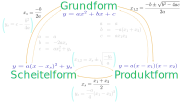
\includegraphics[width=15cm]{allg/funktionen/img/formen/formen.png}
\end{center}

\begin{bemerkung}{}{}
  Das $a$,  ist in allen Formen derselbe Wert und bestimmt die Parabelöffnung.
  \end{bemerkung}
\newpage

\textbf{Grundform aus Scheitelform} (einfaches Ausmultiplizieren). Beispiel:
$$y=2(x-3)^2-4 = 2(x^2-6x+9)-4=2x^2-12x+14$$

\begin{tabular}{rcl}
$a(x-x_S)^2+y_S$ &=& $ax^2-2ax_Sx + (ax_S^2+y_S)$\\
  $a$ &=& $a$ \\
  $b$ &=& $-2ax_S$\\
  $c$ &=& $ax_S^2+y_S$
\end{tabular}


\textbf{Grundform aus Produktform} (einfaches Ausmultiplizieren). Beispiel
$$y=2(x+3)(x-4)=2(x^2 +(3-4)x - 12) = 2x^2-x-24$$

\begin{tabular}{rcl}
  $a(x-x_1)(x-x_2)$ &=& $ax^2 - a(x_1+x_2)x + ax_1x_2$\\
  $a$ &=& $a$ \\
  $b$ &=& $-a(x_1+x_2)$\\
  $c$ &=& $ax_1x_2$
\end{tabular}


\textbf{Nullstellenform (Produktform) aus Grundform}:
Gegeben: $y = ax^2 + bx + c$

Nullstellenform: $y = a(x-x_1)\cdot{}(x-x_2)$ mit

$$x_{1,2} = \frac{-b \pm \sqrt{b^2-4ac}}{2a}$$

\begin{beispiel}{}{}
Gegeben $y = 5x^2 - 5x - 30$. Schreiben Sie dies in der Produktform (=
Nullstellenform):
\platzFuerBerechnungen{3.2}\TRAINER{$y = 5(x-3)(x+2)$\vspace{4.2cm}}
\end{beispiel}
\newpage


\textbf{Scheitelform aus Grundform}:
$$x_S=\frac{-b}{2a}$$

$y_S$ einfach durch Einsetzen von $x_S$ in die Grundform:
$$y_S=c-\frac{b^2}{4a}$$
 
\textbf{Scheitelform aus Produktform}: $x_S$ ist der Mittelwert der beiden
Nullstellen:
$$x_S=\frac{x_1+x_2}{2}$$
Danach $y_S$ einfach durch Einsetzen von $x_S$ in die Produktform:
$$y_S=\frac{-a}{4}(x_1-x_2)^2$$

\textbf{Produktform aus Scheitelform}: Einfachster Weg geht über die Grundform oder abgekürzt:
$$x_{1,2} =x_S \pm \sqrt{\frac{-y_S}{a}}$$


\subsection{Aufgaben}

\TALS{\olatLinkArbeitsblatt{Umrechnen der Formen}{https://olat.bbw.ch/auth/RepositoryEntry/572162090/CourseNode/103176133021102}{1., 2., 3. und 8.}}



\newpage

% Bereits in typ I II und III eingebaut
%\subsection{Parabel aus drei Punkten}
Vorzeigeaufgabe Marthaler Algebra S. 272 Aufg. 3. b) 


\subsection*{Aufgaben}

\AadBMTA{272}{3. a) c)}%% war Marthaler S. 187 Aufg. 676 a) und b)
\GESOAadBMTA{???}{???}

\newpage



%\newpage

%

%%%%%%%%%%%%%%%%%%%%%%%%%%%%%%%%%%%%%%%%%%%%%%%%%%%%%%%%%%%%%%%%
\subsection{Extremwertaufgaben}



\subsubsection{Aus alter Maturprüfung}

\aufgabenFarbe{Gegeben ist die Funktion $f(x) = x\cdot{}(3-\sqrt{x})$,
  $x\in[0;\infty[$.\\
  a) Bestimmen Sie die Nullstellen und das  Extremum der Funktion
  $f$.\\
  b) Im ersten Quadranten, zwischen dem  Graphen und der
  $x$-Achse ist ein  rechtwinkliges Dreieck $ABC$ einbeschrieben.  Der
  rechte Winkel ist in der Ecke $B$.  Punkt $A$ liegt im Ursprung, $B$
  auf der  $x$-Achse und $C$ auf dem Graphen von $f$. Berechnen Sie
  die Koordinaten des  Punktes $C$ so, dass der Flächeninhalt des
  Dreiecks maximal wird.
}%% END aufgabenFarbe

    
\bbwCenterGraphic{8cm}{tals/fct3/img/Maximieren.png}
\TNTeop{
   a) solve$(f(x)=0,x)$ Somit sind die Nullstellen bei 0 und 9\\
     $\text{fmax}(f(x),x)$ liefert $x=4$ ist Maximalstelle (und auch
     Maximalwert ($f(4)=4$)\\
   b) $\text{fmax}(0.5\cdot{}x\cdot{}f(x), x)$ liefert $x = 5.76$ und
   $f(5.76) = 3.456$}%% End TNTeop
\newpage
\subsection*{Aufgaben}
\AadBMTA{311}{49.}
\AadBMTA{321}{17.}

%\newpage

\section{Berührende Graphen}\index{Graphen!berührende}\index{berührende Graphen}

\textbf{Einführungsbeispiel}


Gegeben ist die Parabel $f: y=\frac{1}{4}x^2 -\frac12x +\frac14$ und von einer
Geraden $g$ ist der $y$-Achsenabschnitt $b = -2$ gegeben.

Gesucht ist von der Geraden $g$ die Steigung $a$ so, dass die
Gerade die Parabel tangiert; also genau in einem Punkt berührt.

Wo (in welchem Punkt $B=(x_B|y_B)$) tangiert also die Gerade $g$ die Parabel $f$?

In der folgenden Skizze sind drei mögliche Geraden mit $y$-Achsenabschnitt
$-2$ gezeichnet. Nur eine dieser drei Geraden \textit{tangiert} die Parabel.

\bbwGraph{-4}{4}{-3}{5}{
  \draw[thick,color=blue,variable=\x,domain=-3.5:4] plot ({\x},   {0.25*\x*\x -0.5*\x + 0.25});

  \draw[color=red,variable=\x,domain=-3:5] plot ({\x},{2*\x -2});
  \draw[color=red,variable=\x,domain=-3:5] plot ({\x},{0.5*\x - 2});
  \draw[color=cyan,thick,variable=\x,domain=-3:5] plot ({\x},{1*\x  -2});

  \bbwDot{3, 1}{green}{north}{B}

  %%%\draw[thick,color=blue,variable=\x,domain=-1:5] plot ({\x}, {0.5*\x*\x - 2*\x + 3}); 
  %%\draw[color=red,variable=\x,domain=-1:5] plot ({\x},{0.5*\x + 1});
  %%\draw[color=red,variable=\x,domain=-1:5] plot ({\x},{0.5*\x - 1.5});
  %%\draw[color=cyan,thick,variable=\x,domain=-1:6] plot ({\x},{0.5*\x  -0.125});
  %%\bbwDot{2.5, 1.125}{green}{north}{P}
}
\newpage
\textbf{Lösungsidee}: Der gesuchte Parameter ist $a$, die Steigung der
Geraden.

Nun berechne die Schnittpunkte/den Schnittpunkt mit $$f(x) = g(x).$$

Das $a$ ist gefunden, sobald die Gleichung $f(x)=g(x)$ genau eine
Lösung aufweist; dann also, wenn


\TNT{2}{die Diskriminante dieser Gleichung
verschwindet.}

Den $x$-Wert dieses Berührungspunktes nennen wir $x_B$:


Ansatz:

$$f(x_B) = g(x_B)$$

\TNT{4.4}{
 
\begin{tabular}{rclr}
$\frac14x_s^2-\frac12x_s+\frac14$          & $=$ &  $ax_s-2$ & \\
$\frac14x_s^2+(-\frac12-a)x_s + \frac94$   & $=$ & $0$       & (I)\\
\end{tabular}
\vspace{10mm}
}%% END TNT

Die Diskriminante $D=B^2 - 4AC$ muss gleich 0 sein. 

\TNT{7.2}{
$A = \frac14$, $B = -\frac12-a$ und $C = \frac94$.

  $$D=0=B^2-4AC = (-\frac12-a)^2  - (4\cdot{}A\cdot{}C)$$
  $$0 = (a^2+a+\frac14) - (4\cdot\frac14\cdot{}\frac{+9}4)$$
$$\Longrightarrow 0 = a^2 + a - 2$$
$$\Longrightarrow a_1 = 1 \text{ und  } a_2 = -2$$
\vspace{40mm}
}%% END TNT
\newpage

Für den \textbf{Berührungspunkt} $B=(x_B|y_B)$ müssen wir nun nur doch das gefundene
$a$ in die Gleichung (I) einsetzen.


\TNT{6}{
  $$0 = \frac14x_B^2 + (-\frac12 -a ) + \frac94$$

  $$x_B = x_1 = x_2 = \frac{-B \pm\sqrt{D}}{2A} = \frac{-B \pm
    \sqrt{0}}{2A} = \frac{-B}{2A}$$

  $$x_B = \frac{-B}{2A} = \frac{- (-\frac12 - a)}{\frac24} =
  \frac{\frac12 + a}{\frac12} = (\frac12 + a) : \frac12 = (\frac12+a)
  \cdot{} 2 = 1+2a$$
}



1. Fall: ($a_1=1$):

\TNT{6}{
$B_1: a_1 = 1:$
  $$x_B = 1+2a = 1 + 2\cdot{}(1) = 3$$

Das $y$ finden wir einfach durch Einsetzen von $x$ in den
Funktionsterm der Geradengleichung.

$$y_1 = a_1x_1 - 2 = 1\cdot{}3-2 = 1$$
und somit ist
$$B_1 = (3 | 1)$$
}%% END TNT



2. Fall: ($a_1=-2$):


\TNTeop{
$B_2: a_2 = -2:$
  $$x_B = 1+2a = 1 + 2\cdot{}(-2) = 1-4=-3$$


$$y_2 = a_2x_2+b = -2\cdot{}3-2 = 4$$
und somit ist
$$B_2 = (-3 | 4)$$

}%% END TNT
\newpage




\begin{rezept}{Berührende Graphen}{}

  Bei Berührungsaufgaben mit Parabeln hilft i.\,d.\,R. das folgende
  Vorgehen:

  \begin{enumerate}
  \item Funktionsterme Gleichsetzen: $$f(x) = g(x)$$
  \item In Grundform bringen: $$f(x) - g(x) = 0  \hspace{40mm}
    (I)$$
  \item Diskriminante $D = 0 $ setzen, um den Parameterwert zu
    bestimmen.
  \item Gleichung $(I)$ auflösen mit dem Wissen $D=0$.
    $$x_B=x_1=x_2= \frac{-B}{2A}$$

  \item Gefundenen Parameter in $x_B=\frac{-B}{2A}$ einsetzen, um $x$
    des Berührungspunktes zu bestimmen.
  \item Das $y_B$ des Berührungspunktes ermitteln, indem wir $x_B$ in
    $f$ oder $g$ einsetzen.
    \end{enumerate}
\end{rezept}


\TRAINER{(Je nach Zeit wäre 699. a) noch eine Vorzeigeaufgabe.)}

\subsection{Aufgaben}
\TRAINER{Achtung, dass nicht das Gleichungssystem bereits
  nach dem Gleichsetzen der Graphen aufgestellt wird. Erst nach dem
  Null-Setzen der Diskriminante erhalten wir eine gültige Gleichung
  für das Gleichungssystem.}
%%\TALSAadBMTA{190}{698., 702., 703., 705.}
\TALSAadBMTA{277}{30. a), 36. a), 40. a) c), 42. a), 43. a), 44. a)}
\newpage


\subsection{Grenzwerte und Steigungsfunktion (Optional)}

Wie macht das ein CAS, dass es den tiefsten bzw. den höchsten Punkt
einer Funktion bestimmen kann? Hier ein Erklärungsversuch am Beispiel
der quadratischen Funktion.
Betrachten wir die allgemeine quadratische Funktion $$p: y=ax^2 + bx +
c$$
Mit dem selben $a$ und dem selben $b$ kann ich eine Gerade $s$
definieren, die ich die (Tangenten-)\textbf{Steigungsfunktion}\footnote{Diese
  Steigungsfunktion wird in der Mathematik die
  \textbf{Ableitung}\index{Ableitung} genannt. Genau genommen handelt
  es sich nicht um die Steigung der Parabel, sondern um die Steigung
  einer im Punkt $P=(X_P|f(x_P))$ angelegter Tangente.} nenne:
$$s: y= 2ax+b$$
\newpage


Diese Steigungsfunktion $s$ gibt in jedem Punkt $x$ die Steigung einer
Tangente an die Parabel $p$ an.

\begin{beispiel}{Parabel}{}
  Gegeben ist die Parabel $$p: y=2.5x^2 - 3x + 6.5\text{.}$$

  Wo (für welches $x$) hat diese Parabel
  ihren Tiefpunkt? \TRAINER{Scheitelpunkt:}

  $$x_B =   \LoesungsRaumLen{8cm}{\frac{-b}{2a} = \frac{-(-3)}{2\cdot{}2.5} = 0.6}$$

  Dies ist gleichzeitig die Nullstelle der
  Steigungsfunktion:

  $$s: y= \LoesungsRaumLen{3cm}{2\cdot{}2.5x - 3}$$

  Nullstelle von $s$:

  $$x_0 = \LoesungsRaumLen{7cm}{\frac{3}{2\cdot{}2.5} = 0.6}$$

  Wir können damit aber auch die Steigung in einem ganz anderen Punkt
  \zB für $x=10$ berechnen. Die Parabel $p$ hat an der Stelle $x=10$
  die Tangentensteigung, die durch die Steigungsfunktion im Punkt $10$
  ermittelt wird:

  $$s(10) = \LoesungsRaumLen{40mm}{2\cdot{}10\cdot{2.5} - 3 = 47}$$
  
\end{beispiel}
\newpage

\begin{beispiel}{Gerade gesucht}{}
Gegeben ist die Parabel $$p: y=4x^2 -6x + 3\text{.}$$ Gesucht ist die Gerade
$g: y=ax+b$, sodass die Gerade die Parabel bei $x=7$ berührt.

\begin{enumerate}
\item Die Steigungsfunktion $s$ lautet: $$s:
  y=\LoesungsRaumLen{5cm}{2\cdot{}4x - 6}$$
  
\item Für $x=7$ hat die Steigungsfunktion den Wert \LoesungsRaumLen{1cm}{50}, und somit hat
  die Parabel bei $x=7$ die Steigung \LoesungsRaumLen{1cm}{50}.

  
\item Um den Berührungspunkt $B$ zu finden, setzen wir 7 diesen in $p$
  ein
  $$p(7)= \LoesungsRaumLen{5cm}{4\cdot{}49-6\cdot{}7+3 = 157}$$
  und somit ist
  $$B=(\LoesungsRaum{7}|\LoesungsRaum{157})$$
  
\item Die gesuchte Gerade $g: y=ax+b$ hat also auch die Steigung \LoesungsRaum{50}
  und verläuft durch den Berührungspunkt $B=(\LoesungsRaumLen{9mm}{7}|\LoesungsRaumLen{11mm}{157})$. Also
  $$\LoesungsRaumLen{7cm}{157=50\cdot{}7+b}$$

  Somit ist das gesuchte
  $$b = \LoesungsRaumLen{55mm}{157-50\cdot{}7=-193}$$
  
  und die gesuchte Funktionsgleichung der Geraden lautet: $$y = \LoesungsRaumLen{22mm}{50x-193}$$
  \end{enumerate}
\end{beispiel}

\TRAINER{Idee: Auf mm-Papier eine Funktion $y=\frac1{27}x^3-\frac19
  x^2 - \frac89 x$ vorgeben.

Auftrag: Legen Sie in 5 Punkten eine Tangente an die Funktion und
bestimmen Sie deren Steigung.
Tragen Sie die Steigung in ein neues Koordinatensystem ein: $x$-Achse
= $x$ Wert, $y$-Achse = Steigung der Funktion.
$$f' : y = \frac19 (x-1)^2 - 1 $$
}%%
\newpage

\subsubsection{Beweis der Formel der (Tangenten-)Steigungsfunktion}

Betrachten wir auf auf der $x$-Achse zwei benachbarte Punkte $x$ und
$x+\Delta$. Die Funktionswerte lauten $f(x)$ und $f(x+\Delta)$. Die
\textbf{Steigung} kann nun für eine Gerade bestimmt werden durch:

\bbwCenterGraphic{7cm}{tals/fct3/img/Steigungsfunktion.jpg}

$$\frac{f(x+\Delta) - f(x)}{\Delta}$$

Dies gilt für eine Parabel $p: y=ax^2+bx+c$ näherungsweise auch:
$$\frac{f(x+\Delta)-f(x)}{\Delta} = \frac{(a(x+\Delta)^2 + b(x+\Delta)
  + c) - (ax^2 + bx +c)}{\Delta}=2ax+a\Delta+b$$

Wenn wir nun das $\Delta$ gegen Null gehen lassen, also immer kleinere
Werte einsetzen, so verschwindet der Term $a\cdot{}\Delta$ fast und unsere
Formel stimmt annähernd --- jedoch präzise genug, um dies als Beweis
gelten zu lassen.

Ein anderer Beweis wäre die Tangente effektiv einzusetzen und diese so
zu wählen, dass es genau einen Schnittpunkt gibt, was wieder darauf
zurückführt, dass die Diskriminante = Null gesetzt werden muss. Dann
sind wir exakt, aber der Beweis ist ungleich aufwändiger.
\newpage


\newpage


%% Part Trigo I
%%%%%%%%%%%%%%%55
%% Funktionen II TALS Metapackage
\part{Funktionen II}\index{Funktionen!II|textbf}
\renewcommand{\bbwPartID}{FCT2}
%%
%% 2019 07 04 Ph. G. Freimann
%%

\section{Quadratische Funktionen}\index{Funktionen!quadratische}
\sectuntertitel{Geraden im Lande der Parabeln wird dringend angeraten, einen
  Integrationskurs zu besuchen.}
%%%%%%%%%%%%%%%%%%%%%%%%%%%%%%%%%%%%%%%%%%%%%%%%%%%%%%%%%%%%%%%%%%%%%%%%%%%%%%%%%

%%\bbwCenterGraphic{8cm}{tals/fct2/img/lugano2018.jpg}
%%\textit{Bildlegende: Parabeln in Lugano (2018)}
\bbwCenterGraphic{175mm}{tals/fct2/img/paris2022.jpg}
\textit{Bildlegende: Parabeln in den Gärten von Versailles (2022)}

\subsection*{Lernziele}

\begin{itemize}
\item Definition
\item Formen: Scheitel-, Produkt-, Normalform
\item Graphische Darstellung
\item Translationen und Spiegelungen
\end{itemize}

\TadBMTA{260}{15}
%%\TALS{(\cite{frommenwiler17alg} S.183 (Kap. 3.4))}
%%\GESO{(\cite{marthaler21alg}       S.260 (Kap. 15))}

Einstieg: Bilder von Heimgartner/Hunziker.


\textbf{Einstiegsaufgabe: } \aufgabenFarbe{Lösen Sie Aufgaben 1. und 2.
  von Seite 272: Welche der angegebenen Funktionen sind quadratisch?}

\newpage

\subsection{Parabel}\index{Parabel}\index{Normalparabel}

Zeichnen Sie die Funktionen $f: y=x^2$ (= Normalparabel), $y=\frac{1}{3}x^2$

und $y=-0.25\cdot{}x^2$  ins Koordinatensystem:

\bbwGraph{-3}{3}{-3}{7}{
  \TRAINER{\bbwFuncC{\x * \x}{-2.5:2.5}{green}
    \bbwFuncC{-0.25*\x * \x}{-3:3}{green}
    \bbwFuncC{\x * \x / 3}{-3:3}{green}
  }
}


\newpage

\subsection{Grundform}\index{Grundform!quadratische Funktion}\index{Quadratische Funktion!Grundform}
Die Funktion $f(x): x \mapsto y = ax^2 + bx +c$ ist eine
quadratische Funktion in Grundform\index{Grundform!quadratische Funktion}.

Spielen Sie mit \TALS{dem TI-nSpire oder mit} \texttt{geogebra.org} an den Parametern $a$, $b$ und $c$ der Funktionsgleichung $y = a\cdot{}x^2 + b\cdot{} x + c$ herum. Was bewirkt der Parameter

$a$: \LoesungsRaumLang{Parabelöffnung: $|a|$ klein: Breite (weite) Öffnung / $|a|$ groß: Enge, schmale Öffnung. $a < 0$: Parabel ist nach unten geöffnet. $a > 0$: Parabel ist nach oben geöffnet.}

$b$: \LoesungsRaumLang{«Parabelsteigung»\footnote{Mit «Parabelsteigung» ist hier die Steigung der entsprechenden Tangente gemeint.} im Punkt $A(0|c)$}

$c$: \LoesungsRaumLang{$y$-Achsenabschnitt. Damit wird eine Verschiebung der Parabel entlang der $y$-Achse erreicht.}

Versuchen Sie eine Parabel mit Scheitelpunkt $(1|1)$ zu finden\TRAINER{(Lösung: $b=-2a$ und $a+b+c=1$.)}.

\subsection*{Aufgaben}
%%\TALSAadBMTA{184ff}{660. a) c) f), 662. a) b) c) und e)}
\AadBMTA{273}{5., 6., 7., 8. und 9.}
\newpage

\subsection{Vier charakteristische Punkte}
Zeichnen Sie die Funktion
$$p: y = x^2 - 4x + \frac{7}{4}$$

\bbwGraph{-3}{6}{-3}{2}{
\TRAINER{\bbwFunc{\x*\x - 4*\x + 1.75}{-0.2:4}}
}%% end BBW Graph

Wo befinden sich die charakteristischen Punkte?

\TNT{2.4}{\vspace{24mm}}


Die charakteristischen Punkte sind:
\begin{itemize}
\item Schnittpunkt mit $y$-Achse = (\LoesungsRaum{0} | \LoesungsRaum{1.75})
\item Nullstellen: $N_1=(\LoesungsRaum{0.5}| \LoesungsRaum{0}), N_2=( \LoesungsRaum{3.5}|\LoesungsRaum{0})$
\item Scheitelpunkt: $S=(\LoesungsRaum{2}|\LoesungsRaum{-2.25})$
\end{itemize}
 
Wie berechnen sich nun diese Punkte?
\newpage
\subsubsection{Parabelöffnung}
Eigentlich ist die Parabelöffnung kein charakteristischer
Punkt. Dennoch kann man eine $x$-Einheit vom Scheitelpunkt entfernt,
das $a$ der Grundform ($y=ax^2+bx+c$) direkt ablesen. Gehen wir bei
der Normalparabel ($a=1$) vom
Scheitelpunkt um eine Einheit nach rechts, so muss die Parabel um eine
$y$-Einheit nach oben anwachsen.

\TNT{10}{
Parabel durch Scheitelpunkt $P=(-3|1)$ und durch $(-2|2)$ =
verschobene Normalparbel zeichnen.

Parabel mit Scheitelpunkt $P=(2|2)$ durch $(3|0.5)$ zeichnen. Das $a$
ist somit sofort $a=-1.5$ abzulesen.
}

\subsubsection{$y$-Achsenabschnitt}
Genau wie bei der linearen Funktion, gilt für den $y$-Achsenabschnitt,
dass die $x$-Koordinate dieses Punktes Null ist.
$$y = x^2 -4x + 1.75$$
wird mit $x=0$ zu
$y = 1.75$.

Der $y$-Achsenabschnitt ist somit immer das $c$ aus $y = ax^2 + bx +
c$.

\newpage

\subsubsection{Nullstellen}
Wie bei den linearen Funktionen sind auch hier die
Nullstellen die Schnittpunkte mit der $x$-Achse. Dies bedeutet für die
Nullstellen $N(x_0 | y_0)$, dass die $y$-Koordinate = 0 ist. Es gilt
also

$$0 = x^2 - 4 x + \frac{7}{4} $$

Dies ist eine quadratische Gleichung mit den Lösungen:

$$x_{1,2} = \frac{-b \pm \sqrt{b^2-4ac}}{2a}$$ 

\noTRAINER{\platzFuerBerechnungen{2.4}}
\TRAINER{$x_{1} = 0.5; x_{2}=3.5$ (Mitternachtsformel)
  \vspace{3cm}}

\begin{bemerkung}{}{}
  Die Nullstellen der quadratischen Funktion entsprechen den Lösungen
  der zugehörigen quadratischen Funktion (mit $y=0$). Daher gilt
  auch hier: 


  \begin{tabular}{c|p{8cm}}
    Diskriminante $D=b^2-4ac$ > 0 & Es gibt zwei Nullstellen. \\
    \hline\\
    Diskriminante $D=b^2-4ac$ = 0 & Es gibt eine Nullstelle, denn der Scheitelpunkt liegt auf der $x$-Achse.\\
    \hline\\
    Diskriminante $D=b^2-4ac$ < 0 & Es gibt keine Nullstellen, denn die Parabel schneidet die $x$-Achse nicht.\\
  \end{tabular}
  
 \ifisALLINONE{Zum Begriff \textbf{Diskriminante}:  \totalref{diskriminante}}\fi{} 
\end{bemerkung}

\subsection*{Aufgaben}
\AadBMTA{277ff}{28. a) c) }

\newpage



\subsubsection{Scheitelpunkt}\index{Scheitelpunkt}
Der Tief- bzw. Hochpunkt einer Parabel wird \textbf{Scheitelpunkt}
genannt.

Wir berechnen den Scheitelpunkt in zwei Schritten.

\textbf{Erstens:} Wir berechnen den Mittelwert der beiden Nullstellen:
$$x_S := \frac{x_{1} + x_{2}}{2} = \frac{\frac{-b+\sqrt{D}}{2a} + \frac{-b-\sqrt{D}}{2a}}{2} =
\frac{(-b+\sqrt{D}) + (-b-\sqrt{D})}{4a} =\frac{-b}{2a}$$
Dabei ist $D$ die Diskriminante $D=b^2-4ac$.

\platzFuerBerechnungen{2.4}
\TRAINER{$x_S = 2$
\vspace{3cm}}

\textbf{Zweitens:} Wir setzen den gefundenen $x$-Wert
(\LoesungsRaum{2}) in die Funktionsgleichung
ein:
$$y_S = x^2 - 4x + 1.75$$
$$y_S = (\LoesungsRaum{2})^2 - 4\cdot{}(\LoesungsRaum{2}) + 1.75$$

Wir erhalten für den Scheitelpunkt $S$: $S=(x_S | y_S) = (\LoesungsRaum{2} | \LoesungsRaum{-2.25})$.

\begin{gesetz}{Scheitelpunkt}{}
  Der Scheitelpunkt $S$ einer Parabel in der Grundform ($y=ax^2+bx+c$) kann wie folgt
  berechnet werden:

  $$S=\left(\frac{-b}{2a}\middle|\frac{4ac-b^2}{4a}\right)$$

  (Bem.: Der $y$-Wert kann einfach durch Einsetzen des $x$-Wertes in
  die Funktionsgleichnug gefunden werden.)
  \end{gesetz}
  
\subsection*{Aufgaben}
%%\TALSAadBMTA{184ff}{665. a) b) c) 666. a) b) c) e) f) g)}
\AadBMTA{273}{4. (=Aufg. 22. S. 276)}

\newpage

\subsection{Bestimmen der Funktionsgleichung}
\TALS{S. 187 Kap. 3.4.3}

\subsubsection{Referenzaufgaben}

\textbf{TYP I}

Gegeben ist ein Punkt $P$ mit den Koordinaten $(2.3 | -1.5)$. Gesucht ist die reinquadratische Funktion $f: y=a\cdot{}x^2$, welche durch diesen Punkt geht.
Machen Sie vorab eine Skizze.

\bbwGraph{-3}{3}{-2}{1}{
  \TRAINER{\bbwFunc{-0.2836 * \x * \x}{-2.5:2.5}
    \bbwDot{2.3,-1.5}{blue}{west}{P}
  }%% end TRAINER
}%% end BBW Graph

\platzFuerBerechnungen{3.6}

\TRAINER{Idee: Punkt einsetzen: $-1.5 = a\cdot{}(2.3)^2$. Das Auf"|lösen dieser Gleichung liefert $a = \frac{-1.5}{2.3^2}$. Dies liefert $a\approx -0.2836$}

Weitere «TYP 1» Aufgaben wären z. B. $y = 3x^2 - bx + 4$ oder $y=2x^2
-7x + c$ mit anderen Worten alle Parabeln mit genau \textbf{einem}
Parameter, daher «Typ 1».

\newpage



\textbf{TYP II}

Gegeben sind zwei Punkte und wir haben zwei Unbekannte.

\begin{rezept}{}{}
  Gesucht sind $a$ und $c$ aus $y = ax^2 + c$ bei den gegebenen
  Punkten $(7|5)$ und $(2|-4)$.

  Wir lösen dies auch durch Einsetzen der Punkte in die
  Funktionsgleichung und wir erhalten zwei Gleichungen:


  \begin{tabular}{c | r  c  r |}
    (I)  &  $5$ & = & $(7)^2\cdot{} a + c$ \\
    (II) & $-4$ & = &  $(2)^2\cdot{} a + c$ \\
  \end{tabular}

  Durch Subtrahieren der Gleichungen erhalten wir

  \begin{tabular}{c | r  c  r | c}
    (I)  &  $5$ & = & $49\cdot{} a + c$ & \,\\
    (II) & $-4$ & = &  $4\cdot{} a + c$ & $\ominus$\\
  \end{tabular}

  $$9 = 45a$$ und somit
  $$a =\frac{1}{5}.$$

  Dieses $a$ (= $\frac{1}{5}$) setzen wir nun in eine der Gleichungen
  (\zB (I)) ein und erhalten
  $$5=49\cdot{}\frac{1}{5} + c$$
  und nach Auf"|lösen erhalten wir $c=\frac{-24}{5}$.

  Die gesuchte Gleichung lautet also:

  $$y = \frac{1}{5}x^2 - \frac{24}{5}$$
\end{rezept}

Probe durch Einsetzen der $x$-Werte der Punkte in die gefundene Funktionsgleichung:

\TNTeop{}
%%\newpage

\begin{beispiel}{}{}
  Anstelle von $a$ und $c$ können natürlich auch $a$ und $b$ gesucht
  sein. Daher eine zweite Aufgabe.

  Gesucht sind $a$ und $b$ aus $y = ax^2 + bx$ bei den gegebenen

  Punkten $(2|-6)$ und $(-3|5)$.

  Wir lösen dies wiederum durch Einsetzen der Punkte in die
  Funktionsgleichung und wir erhalten die beiden Gleichungen, welche
  wir durch das Additionsverfahren lösen können:

  \begin{tabular}{c | r  c  r | c}
    (I)  &  $-6$ & = & $4a + 2b$ & $\cdot{} 3$ \\
    (II) &   $5$ & = & $9a - 3b$ & $\cdot{} 2$ \\
  \end{tabular}

  somit:
  
  \begin{tabular}{c | r  c  r | c}
    (I')  & $-18$ & = & $12a + 6b$ &\, \\
     \,   & \,    & \,&   \,       & $\oplus$\\
    (II') &  $10$ & = & $18a - 6b$ &\, \\
  \end{tabular}

  Nach Addition der Gleichungen erhalten wir

  $$-8 = 30a$$

  was uns zu $a=\frac{-4}{15}$ bringt.

Dieses $a$ können wir nun wieder in eine der beiden Gleichungen
einsetzen (\zB in (I)):

$$-6=4\cdot{}\frac{-4}{15} + 2b$$

Das Auf"|lösen obiger Gleichung liefert nach Kürzen: $b=\frac{-37}{15}$.

Die gesuchte Funktionsgleichung lautet also

$$y = \frac{-4}{15} x^2 - \frac{37}{15} x.$$

\end{beispiel}

Auch bei «Typ II» kann natürlich jede \textbf{zwei}parametrige quadratische
Funktion herhalten, wie \zB $y=-6cx^2 + bx - c$ durch \textbf{zwei}
gegebene Punkte.
\newpage


\textbf{TYP III}: Gegeben sind hier drei Punkte, wir haben aber auch
drei Unbekannte in $y = ax^2 + bx + c$. Die Punkte sind hier
(1|3), (2|3.5) und (-3|11).

Durch Einsetzen der drei Punkte je in die Funktionsgleichung erhalten
wir drei Gleichungen:

\begin{tabular}{c|r c rcrcr|}
  (I)   & 3   & = & $(1)^2\cdot{}a$  &$+$& $(1)\cdot{}b$  &$+$& c \\ 
  (II)  & 3.5 & = & $(2)^2\cdot{}a$  &$+$& $(2)\cdot{}b$  &$+$& c \\ 
  (III) & 11  & = & $(-3)^2\cdot{}a$ &$+$& $(-3)\cdot{}b$ &$+$& c \\ 
\end{tabular}

Vereinfachen:

\begin{tabular}{c|r c rcrcr|}
  (I)   & 3   & = & $a$  &$+$& $b$  &$+$& c \\ 
  (II)  & 3.5 & = & $4a$ &$+$& $2b$ &$+$& c \\ 
  (III) & 11  & = & $9a$ &$-$& $3b$ &$+$& c \\ 
\end{tabular}

Nun finden wir $a$, indem wir zunächst $c$ durch Subtraktion
eliminieren:

\begin{tabular}{l|r c rcr|}
  (IV) = (II) -   (I) & 0.5  & = & $3a$ &$+$& $b$ \\ 
  (V)  = (III) - (II) & 7.5  & = & $5a$ &$-$& $5b$ \\ 
\end{tabular}

Multiplizieren wir nun die Gleichung (IV) mit 5, so erhalten wir

\begin{tabular}{r|r c rcr|}
  5$\cdot{}$(IV)  & 2.5  & = & $15a$ &$+$& $5b$ \\ 
  (V)             & 7.5  & = & $5a$  &$-$& $5b$ \\ 
\end{tabular}

Durch Addition der beiden Gleichungen (IV) und (V) erhalten wir

$10 = 20a$ oder $a = \frac{1}{2}$.

Um $b$ zu finden, setzen wir $a = \frac{1}{2}$ in (V) ein: $7.5 =
5\cdot{}\frac{1}{2} - 5b$.

Auf"|lösen nach $b$ ergibt $b = -1$.

Zu guter Letzt setzen wir $a = \frac{1}{2}$ und $b=-1$ in die
Gleichung (I) ein, um noch $c$ zu erhalten:

$$3 = a + b + c = \frac{1}{2} - 1 + c$$

Somit ist $c=3.5$ und die Funktionsgleichung lautet:

$$y = \frac{1}{2}x^2 - x + 3.5$$


\TALS{\subsection*{Aufgaben}}
%%\TALSAadBMTA{187ff}{676. a) c), 682., 684.}
\AadBMTA{272}{3. a) c), 20. a) c), 21., 22., 24. a), 25. b)}
\newpage


\subsection{Computer Algebra Systeme (CAS)}\index{CAS}
Das eben gezeigte Beispiel wird in der Praxis meist nicht von Hand,
sondern mit einem Computer-Algebra-System, kurz CAS, gelöst:

\paragraph{Aufgabenstellung}
Gegeben sind wieder drei Punkte (1|3), (2|3.5) und (-3|11).
Gesucht ist die Parabel $y = ax^2 + bx + c$, welche durch die drei
Punkte geht.

Dies wird mit dem \tinspire{} wie folgt gelöst:
\begin{itemize}
\item Definiere die Funktionsgleichung mit
  Parametern\footnote{\tinspire Regel: $ax\ne a\cdot{} x$}:\\
  $$f(x) := a\cdot{}x^2 + b\cdot{}x + c$$
\item Definiere das Gleichungssystem:
  $$gls := \left\{ \begin{array}{l}
    f(1) = 3\\
    f(2) = 3.5\\
    f(-3)= 11\\
  \end{array}\right.$$
\item Löse das Gleichungssystem:
  $$solve(gls,\{a, b, c\})$$
\end{itemize}

\subsection*{Aufgaben}
\AadBMTA{272}{3. b) d)}

\newpage

\subsection{Formen der quadratischen Funktion}
\subsubsection{Nullstellenform}\index{Nullstellenform}

Die \textbf{Nullstellenform} wird auch  «faktorisierte Form» oder
«Produktform» genannt.\index{faktorisierte Form}\index{Produktform}

Beachten Sie die folgende quadr. Funktionsgleichung:

$$y = 3.1(x-5)(x+6)$$

Dies ist eine quadratische Funktion in der sogenannten
\textbf{Nullstellenform}, denn die Nullstellen (hier $x_0 = 5$ oder
$x_0 = -6$) können direkt aus der Funktionsgleichung abgelesen werden.
Wenn wir $y=0$ in die Gleichung setzen (Nullstelle),

$$0 = 3.1(x-5)(x+6)$$
so wird die Gleichung genau dann wahr, wenn (mind.) einer der beiden Klammerausdrücke rechts
gleich Null ist. Die Parabelöffnung (hier 3.1) kann dabei beliebig variieren und ist (neben den Nullstellen) der einzige Parameter.

Die Nullstellenform lautet

\begin{gesetz}{}{}

  $$y = a(x-x_1)\cdot{}(x-x_2)$$

  \end{gesetz}

wobei $x_1$ und $x_2$ die Nullstellen der Parabel bezeichnen. 
\newpage


\subsubsection*{Referenzaufgabe zur Nullstellenform}

\noTRAINER{\bbwGraphic{16cm}{tals/fct2/img/BrunnenNullstellenformOhneKoordinatensystem.png}}
\TRAINER{\bbwGraphic{16cm}{tals/fct2/img/BrunnenNullstellenformMitKoordinatensystem.png}}

Ein parabelförmiger Wasserstrahl spritzt ebenerdig aus einem Brunnen und trifft 7m von der Düse entfernt wieder auf dem Boden auf.
Das Wasser steigt also erst gleich hoch an, wie es danach wieder «herunterfällt».
Dabei wird gemessen, dass 1m von der Düse entfernt der Wasserstrahl 84cm über Boden verläuft.
Können Sie aufrecht unter dem Wasserstrahl hindurchgehen?

Tipp: Skizze und  die Parabelgleichung in Nullstellenform aufschreiben. Die Düse ist der Ursprung der Koordinatensystems.\\

\TNT{5.2}{Die Funktionsgleichung lautet $y=a(x-x_1)(x-x2)$.\\
  Mit den Nullstellen $x_1=0$ und $x_2=7$.\\
  Wir setzen den gemessenen Punkt (1|0.84) in die Gleichung ein und erhalten $0.84 = a\cdot{}(1-0)(1-7)$.\\
  Daraus ergibt sich $a=0.84/(-6) = -0.14 $.\\
  Nun setzen wir 3.5 Meter in die Funktionsgleichung $y = -0.14(x-0)(x-7)$ ein: und erhalten $y=-01.4\cdot{}3.5\cdot{}(-3.5) = 1.715m$; das ist die höchste Parabelstelle.}


\subsection*{Aufgaben}%% Nullstellenform
%%\TALSAadBMTA{185}{663, 678., 680.}
\TALSAadBMTA{277}{30. a) b), 31. b)}
\newpage

%%\TRAINER{\, \newpage}
\subsubsection{Scheitelform}\index{Scheitelform!der quadratischen
  Funktion}
Einstieg: Wo hat die Parabel $f: y=3.6(x-4)^2 + 5$ ihren
Scheitelpunkt?

\TNT{4.4}{CAS: bei $x_S = 4$ und $y_S= 5$; völlig irrelevant ist die 3.6.}

Ist eine quadratische Funktion in der Form
\begin{gesetz}{}{}
$$y = a(x-x_S)^2 + y_S$$
\end{gesetz}
gegeben, so sprechen wir von der \textbf{Scheitelform} oder Scheitelpunktsform.
Das liegt daran, dass diese Parabel ihren Scheitelpunkt bei
$(x_S|y_S)$ hat.

Setzen wir für $x$ = $x_S$ in die Funktionsgleichung, so erhalten wir
gerade die $y$-Koordinate des Scheitelpunktes. Je weiter wir uns nun
mit $x$ von $x_S$ wegbewegen, umso größer wird der Term $(x-x_S)^2$
und zwar in egal welcher Richtung wir uns von $x_S$ wegbewegen, die
$y$-Koordinate verhält sich in beiden Fällen symmetrisch.

Prüfen Sie dies mit TI-nSpire oder \texttt{geogebra.org} an der Funktion

$$y = a\cdot{}(x-p)^2 + q$$

Definieren Sie dabei auch den Punkt $S=(p|q)$. Spielen Sie nun mit
$a$, $p$ und $q$. Was bewirken die Änderungen?
\newpage


\subsubsection{Referenzaufgabe Scheitelform}
Von einer Parabel ist der Scheitel $S(2|3)$ gegeben. Ebenfalls ist bekannt, dass die Parabel durch den Punkt $P\left(-\frac{1}{2}\middle|1\right)$ geht.

  Berechnen Sie die Funktionsgleichung in der Grundform $y = ax^2 + bx + c$. Tipp:
  Schreiben Sie die Funktionsgleichung in der Form $y=a(x - x_S)^2 +  y_S$ und setzen anschließend den Punkt $P$ ein.

  \platzFuerBerechnungen{8.0}%%
  \TRAINER{
    Ansatz:
    $$y = a(x-2)^2 + 3$$
    Jetzt $P$ einsetzen:
    $$1 = a(-\frac{1}{2} - 2)^2 + 3 $$
    Nach $a$ auf"|lösen ergibt:
    $$a=-0.32 (=\frac{-2}{2.5^2})$$
    Nun setzen wir $a=-0.32$ in die Funktionsgleichung $y=a(x-2)^2+3$
    ein:
    $$y=-0.32(x-2)^2+3$$
    und quadrieren das Binom, um die geforderte Grundform zu erhalten:
    $$y = -0.32(x^2 - 4x + 4) + 3 = -0.32x^2 + 1.28x + 1.72$$
  }%%end TRAINER%%

  \subsection*{Aufgabe}
  \AadBMTA{277}{29. a) c) e), 32. a), 33.}
%%  \TALSAadBMTA{185}{679. a), 681., 695., 684. a), 700., 694., 686.(*) und  664.}}

\newpage


\subsection{Umrechnungen der Formen}\index{Formen!der quadratischen Funktion}\index{Quadratische Funktion!Formen}

Nochmals die drei Formen im Überblick:


\begin{tabular}{c|l}
  Form & Funktionsgleichung\\
  \hline\\
  Normalform/Grundform & $f: y= ax^2 + bx + c$\\
  \hline\\
  Nullstellenform, faktorisierte Form oder Produktform & $f: y=a(x-x_0)(x-x_1)$\\
  \hline\\
  Scheitelform & $f: y=a(x-x_S)^2+y_S$\\
  \hline%%
\end{tabular}


\subsubsection{Umrechnungen zwischen den Formen}\index{Umrechnungen!quadratische Funktion}\index{Quadratische Funktion!Umrechnungen}

\begin{center}
  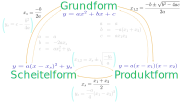
\includegraphics[width=15cm]{allg/funktionen/img/formen/formen.png}
\end{center}

\begin{bemerkung}{}{}
  Das $a$,  ist in allen Formen derselbe Wert und bestimmt die Parabelöffnung.
  \end{bemerkung}
\newpage

\textbf{Grundform aus Scheitelform} (einfaches Ausmultiplizieren). Beispiel:
$$y=2(x-3)^2-4 = 2(x^2-6x+9)-4=2x^2-12x+14$$

\begin{tabular}{rcl}
$a(x-x_S)^2+y_S$ &=& $ax^2-2ax_Sx + (ax_S^2+y_S)$\\
  $a$ &=& $a$ \\
  $b$ &=& $-2ax_S$\\
  $c$ &=& $ax_S^2+y_S$
\end{tabular}


\textbf{Grundform aus Produktform} (einfaches Ausmultiplizieren). Beispiel
$$y=2(x+3)(x-4)=2(x^2 +(3-4)x - 12) = 2x^2-x-24$$

\begin{tabular}{rcl}
  $a(x-x_1)(x-x_2)$ &=& $ax^2 - a(x_1+x_2)x + ax_1x_2$\\
  $a$ &=& $a$ \\
  $b$ &=& $-a(x_1+x_2)$\\
  $c$ &=& $ax_1x_2$
\end{tabular}


\textbf{Nullstellenform (Produktform) aus Grundform}:
Gegeben: $y = ax^2 + bx + c$

Nullstellenform: $y = a(x-x_1)\cdot{}(x-x_2)$ mit

$$x_{1,2} = \frac{-b \pm \sqrt{b^2-4ac}}{2a}$$

\begin{beispiel}{}{}
Gegeben $y = 5x^2 - 5x - 30$. Schreiben Sie dies in der Produktform (=
Nullstellenform):
\platzFuerBerechnungen{3.2}\TRAINER{$y = 5(x-3)(x+2)$\vspace{4.2cm}}
\end{beispiel}
\newpage


\textbf{Scheitelform aus Grundform}:
$$x_S=\frac{-b}{2a}$$

$y_S$ einfach durch Einsetzen von $x_S$ in die Grundform:
$$y_S=c-\frac{b^2}{4a}$$
 
\textbf{Scheitelform aus Produktform}: $x_S$ ist der Mittelwert der beiden
Nullstellen:
$$x_S=\frac{x_1+x_2}{2}$$
Danach $y_S$ einfach durch Einsetzen von $x_S$ in die Produktform:
$$y_S=\frac{-a}{4}(x_1-x_2)^2$$

\textbf{Produktform aus Scheitelform}: Einfachster Weg geht über die Grundform oder abgekürzt:
$$x_{1,2} =x_S \pm \sqrt{\frac{-y_S}{a}}$$


\subsection{Aufgaben}

\TALS{\olatLinkArbeitsblatt{Umrechnen der Formen}{https://olat.bbw.ch/auth/RepositoryEntry/572162090/CourseNode/103176133021102}{1., 2., 3. und 8.}}



\newpage

% Bereits in typ I II und III eingebaut
%\subsection{Parabel aus drei Punkten}
Vorzeigeaufgabe Marthaler Algebra S. 272 Aufg. 3. b) 


\subsection*{Aufgaben}

\AadBMTA{272}{3. a) c)}%% war Marthaler S. 187 Aufg. 676 a) und b)
\GESOAadBMTA{???}{???}

\newpage



%\newpage

%

%%%%%%%%%%%%%%%%%%%%%%%%%%%%%%%%%%%%%%%%%%%%%%%%%%%%%%%%%%%%%%%%
\subsection{Extremwertaufgaben}



\subsubsection{Aus alter Maturprüfung}

\aufgabenFarbe{Gegeben ist die Funktion $f(x) = x\cdot{}(3-\sqrt{x})$,
  $x\in[0;\infty[$.\\
  a) Bestimmen Sie die Nullstellen und das  Extremum der Funktion
  $f$.\\
  b) Im ersten Quadranten, zwischen dem  Graphen und der
  $x$-Achse ist ein  rechtwinkliges Dreieck $ABC$ einbeschrieben.  Der
  rechte Winkel ist in der Ecke $B$.  Punkt $A$ liegt im Ursprung, $B$
  auf der  $x$-Achse und $C$ auf dem Graphen von $f$. Berechnen Sie
  die Koordinaten des  Punktes $C$ so, dass der Flächeninhalt des
  Dreiecks maximal wird.
}%% END aufgabenFarbe

    
\bbwCenterGraphic{8cm}{tals/fct3/img/Maximieren.png}
\TNTeop{
   a) solve$(f(x)=0,x)$ Somit sind die Nullstellen bei 0 und 9\\
     $\text{fmax}(f(x),x)$ liefert $x=4$ ist Maximalstelle (und auch
     Maximalwert ($f(4)=4$)\\
   b) $\text{fmax}(0.5\cdot{}x\cdot{}f(x), x)$ liefert $x = 5.76$ und
   $f(5.76) = 3.456$}%% End TNTeop
\newpage
\subsection*{Aufgaben}
\AadBMTA{311}{49.}
\AadBMTA{321}{17.}

%\newpage

\section{Berührende Graphen}\index{Graphen!berührende}\index{berührende Graphen}

\textbf{Einführungsbeispiel}


Gegeben ist die Parabel $f: y=\frac{1}{4}x^2 -\frac12x +\frac14$ und von einer
Geraden $g$ ist der $y$-Achsenabschnitt $b = -2$ gegeben.

Gesucht ist von der Geraden $g$ die Steigung $a$ so, dass die
Gerade die Parabel tangiert; also genau in einem Punkt berührt.

Wo (in welchem Punkt $B=(x_B|y_B)$) tangiert also die Gerade $g$ die Parabel $f$?

In der folgenden Skizze sind drei mögliche Geraden mit $y$-Achsenabschnitt
$-2$ gezeichnet. Nur eine dieser drei Geraden \textit{tangiert} die Parabel.

\bbwGraph{-4}{4}{-3}{5}{
  \draw[thick,color=blue,variable=\x,domain=-3.5:4] plot ({\x},   {0.25*\x*\x -0.5*\x + 0.25});

  \draw[color=red,variable=\x,domain=-3:5] plot ({\x},{2*\x -2});
  \draw[color=red,variable=\x,domain=-3:5] plot ({\x},{0.5*\x - 2});
  \draw[color=cyan,thick,variable=\x,domain=-3:5] plot ({\x},{1*\x  -2});

  \bbwDot{3, 1}{green}{north}{B}

  %%%\draw[thick,color=blue,variable=\x,domain=-1:5] plot ({\x}, {0.5*\x*\x - 2*\x + 3}); 
  %%\draw[color=red,variable=\x,domain=-1:5] plot ({\x},{0.5*\x + 1});
  %%\draw[color=red,variable=\x,domain=-1:5] plot ({\x},{0.5*\x - 1.5});
  %%\draw[color=cyan,thick,variable=\x,domain=-1:6] plot ({\x},{0.5*\x  -0.125});
  %%\bbwDot{2.5, 1.125}{green}{north}{P}
}
\newpage
\textbf{Lösungsidee}: Der gesuchte Parameter ist $a$, die Steigung der
Geraden.

Nun berechne die Schnittpunkte/den Schnittpunkt mit $$f(x) = g(x).$$

Das $a$ ist gefunden, sobald die Gleichung $f(x)=g(x)$ genau eine
Lösung aufweist; dann also, wenn


\TNT{2}{die Diskriminante dieser Gleichung
verschwindet.}

Den $x$-Wert dieses Berührungspunktes nennen wir $x_B$:


Ansatz:

$$f(x_B) = g(x_B)$$

\TNT{4.4}{
 
\begin{tabular}{rclr}
$\frac14x_s^2-\frac12x_s+\frac14$          & $=$ &  $ax_s-2$ & \\
$\frac14x_s^2+(-\frac12-a)x_s + \frac94$   & $=$ & $0$       & (I)\\
\end{tabular}
\vspace{10mm}
}%% END TNT

Die Diskriminante $D=B^2 - 4AC$ muss gleich 0 sein. 

\TNT{7.2}{
$A = \frac14$, $B = -\frac12-a$ und $C = \frac94$.

  $$D=0=B^2-4AC = (-\frac12-a)^2  - (4\cdot{}A\cdot{}C)$$
  $$0 = (a^2+a+\frac14) - (4\cdot\frac14\cdot{}\frac{+9}4)$$
$$\Longrightarrow 0 = a^2 + a - 2$$
$$\Longrightarrow a_1 = 1 \text{ und  } a_2 = -2$$
\vspace{40mm}
}%% END TNT
\newpage

Für den \textbf{Berührungspunkt} $B=(x_B|y_B)$ müssen wir nun nur doch das gefundene
$a$ in die Gleichung (I) einsetzen.


\TNT{6}{
  $$0 = \frac14x_B^2 + (-\frac12 -a ) + \frac94$$

  $$x_B = x_1 = x_2 = \frac{-B \pm\sqrt{D}}{2A} = \frac{-B \pm
    \sqrt{0}}{2A} = \frac{-B}{2A}$$

  $$x_B = \frac{-B}{2A} = \frac{- (-\frac12 - a)}{\frac24} =
  \frac{\frac12 + a}{\frac12} = (\frac12 + a) : \frac12 = (\frac12+a)
  \cdot{} 2 = 1+2a$$
}



1. Fall: ($a_1=1$):

\TNT{6}{
$B_1: a_1 = 1:$
  $$x_B = 1+2a = 1 + 2\cdot{}(1) = 3$$

Das $y$ finden wir einfach durch Einsetzen von $x$ in den
Funktionsterm der Geradengleichung.

$$y_1 = a_1x_1 - 2 = 1\cdot{}3-2 = 1$$
und somit ist
$$B_1 = (3 | 1)$$
}%% END TNT



2. Fall: ($a_1=-2$):


\TNTeop{
$B_2: a_2 = -2:$
  $$x_B = 1+2a = 1 + 2\cdot{}(-2) = 1-4=-3$$


$$y_2 = a_2x_2+b = -2\cdot{}3-2 = 4$$
und somit ist
$$B_2 = (-3 | 4)$$

}%% END TNT
\newpage




\begin{rezept}{Berührende Graphen}{}

  Bei Berührungsaufgaben mit Parabeln hilft i.\,d.\,R. das folgende
  Vorgehen:

  \begin{enumerate}
  \item Funktionsterme Gleichsetzen: $$f(x) = g(x)$$
  \item In Grundform bringen: $$f(x) - g(x) = 0  \hspace{40mm}
    (I)$$
  \item Diskriminante $D = 0 $ setzen, um den Parameterwert zu
    bestimmen.
  \item Gleichung $(I)$ auflösen mit dem Wissen $D=0$.
    $$x_B=x_1=x_2= \frac{-B}{2A}$$

  \item Gefundenen Parameter in $x_B=\frac{-B}{2A}$ einsetzen, um $x$
    des Berührungspunktes zu bestimmen.
  \item Das $y_B$ des Berührungspunktes ermitteln, indem wir $x_B$ in
    $f$ oder $g$ einsetzen.
    \end{enumerate}
\end{rezept}


\TRAINER{(Je nach Zeit wäre 699. a) noch eine Vorzeigeaufgabe.)}

\subsection{Aufgaben}
\TRAINER{Achtung, dass nicht das Gleichungssystem bereits
  nach dem Gleichsetzen der Graphen aufgestellt wird. Erst nach dem
  Null-Setzen der Diskriminante erhalten wir eine gültige Gleichung
  für das Gleichungssystem.}
%%\TALSAadBMTA{190}{698., 702., 703., 705.}
\TALSAadBMTA{277}{30. a), 36. a), 40. a) c), 42. a), 43. a), 44. a)}
\newpage


\subsection{Grenzwerte und Steigungsfunktion (Optional)}

Wie macht das ein CAS, dass es den tiefsten bzw. den höchsten Punkt
einer Funktion bestimmen kann? Hier ein Erklärungsversuch am Beispiel
der quadratischen Funktion.
Betrachten wir die allgemeine quadratische Funktion $$p: y=ax^2 + bx +
c$$
Mit dem selben $a$ und dem selben $b$ kann ich eine Gerade $s$
definieren, die ich die (Tangenten-)\textbf{Steigungsfunktion}\footnote{Diese
  Steigungsfunktion wird in der Mathematik die
  \textbf{Ableitung}\index{Ableitung} genannt. Genau genommen handelt
  es sich nicht um die Steigung der Parabel, sondern um die Steigung
  einer im Punkt $P=(X_P|f(x_P))$ angelegter Tangente.} nenne:
$$s: y= 2ax+b$$
\newpage


Diese Steigungsfunktion $s$ gibt in jedem Punkt $x$ die Steigung einer
Tangente an die Parabel $p$ an.

\begin{beispiel}{Parabel}{}
  Gegeben ist die Parabel $$p: y=2.5x^2 - 3x + 6.5\text{.}$$

  Wo (für welches $x$) hat diese Parabel
  ihren Tiefpunkt? \TRAINER{Scheitelpunkt:}

  $$x_B =   \LoesungsRaumLen{8cm}{\frac{-b}{2a} = \frac{-(-3)}{2\cdot{}2.5} = 0.6}$$

  Dies ist gleichzeitig die Nullstelle der
  Steigungsfunktion:

  $$s: y= \LoesungsRaumLen{3cm}{2\cdot{}2.5x - 3}$$

  Nullstelle von $s$:

  $$x_0 = \LoesungsRaumLen{7cm}{\frac{3}{2\cdot{}2.5} = 0.6}$$

  Wir können damit aber auch die Steigung in einem ganz anderen Punkt
  \zB für $x=10$ berechnen. Die Parabel $p$ hat an der Stelle $x=10$
  die Tangentensteigung, die durch die Steigungsfunktion im Punkt $10$
  ermittelt wird:

  $$s(10) = \LoesungsRaumLen{40mm}{2\cdot{}10\cdot{2.5} - 3 = 47}$$
  
\end{beispiel}
\newpage

\begin{beispiel}{Gerade gesucht}{}
Gegeben ist die Parabel $$p: y=4x^2 -6x + 3\text{.}$$ Gesucht ist die Gerade
$g: y=ax+b$, sodass die Gerade die Parabel bei $x=7$ berührt.

\begin{enumerate}
\item Die Steigungsfunktion $s$ lautet: $$s:
  y=\LoesungsRaumLen{5cm}{2\cdot{}4x - 6}$$
  
\item Für $x=7$ hat die Steigungsfunktion den Wert \LoesungsRaumLen{1cm}{50}, und somit hat
  die Parabel bei $x=7$ die Steigung \LoesungsRaumLen{1cm}{50}.

  
\item Um den Berührungspunkt $B$ zu finden, setzen wir 7 diesen in $p$
  ein
  $$p(7)= \LoesungsRaumLen{5cm}{4\cdot{}49-6\cdot{}7+3 = 157}$$
  und somit ist
  $$B=(\LoesungsRaum{7}|\LoesungsRaum{157})$$
  
\item Die gesuchte Gerade $g: y=ax+b$ hat also auch die Steigung \LoesungsRaum{50}
  und verläuft durch den Berührungspunkt $B=(\LoesungsRaumLen{9mm}{7}|\LoesungsRaumLen{11mm}{157})$. Also
  $$\LoesungsRaumLen{7cm}{157=50\cdot{}7+b}$$

  Somit ist das gesuchte
  $$b = \LoesungsRaumLen{55mm}{157-50\cdot{}7=-193}$$
  
  und die gesuchte Funktionsgleichung der Geraden lautet: $$y = \LoesungsRaumLen{22mm}{50x-193}$$
  \end{enumerate}
\end{beispiel}

\TRAINER{Idee: Auf mm-Papier eine Funktion $y=\frac1{27}x^3-\frac19
  x^2 - \frac89 x$ vorgeben.

Auftrag: Legen Sie in 5 Punkten eine Tangente an die Funktion und
bestimmen Sie deren Steigung.
Tragen Sie die Steigung in ein neues Koordinatensystem ein: $x$-Achse
= $x$ Wert, $y$-Achse = Steigung der Funktion.
$$f' : y = \frac19 (x-1)^2 - 1 $$
}%%
\newpage

\subsubsection{Beweis der Formel der (Tangenten-)Steigungsfunktion}

Betrachten wir auf auf der $x$-Achse zwei benachbarte Punkte $x$ und
$x+\Delta$. Die Funktionswerte lauten $f(x)$ und $f(x+\Delta)$. Die
\textbf{Steigung} kann nun für eine Gerade bestimmt werden durch:

\bbwCenterGraphic{7cm}{tals/fct3/img/Steigungsfunktion.jpg}

$$\frac{f(x+\Delta) - f(x)}{\Delta}$$

Dies gilt für eine Parabel $p: y=ax^2+bx+c$ näherungsweise auch:
$$\frac{f(x+\Delta)-f(x)}{\Delta} = \frac{(a(x+\Delta)^2 + b(x+\Delta)
  + c) - (ax^2 + bx +c)}{\Delta}=2ax+a\Delta+b$$

Wenn wir nun das $\Delta$ gegen Null gehen lassen, also immer kleinere
Werte einsetzen, so verschwindet der Term $a\cdot{}\Delta$ fast und unsere
Formel stimmt annähernd --- jedoch präzise genug, um dies als Beweis
gelten zu lassen.

Ein anderer Beweis wäre die Tangente effektiv einzusetzen und diese so
zu wählen, dass es genau einen Schnittpunkt gibt, was wieder darauf
zurückführt, dass die Diskriminante = Null gesetzt werden muss. Dann
sind wir exakt, aber der Beweis ist ungleich aufwändiger.
\newpage


\newpage


%% Part Trigo II
%%%%%%%%%%%%%%%55
%% Funktionen II TALS Metapackage
\part{Funktionen II}\index{Funktionen!II|textbf}
\renewcommand{\bbwPartID}{FCT2}
%%
%% 2019 07 04 Ph. G. Freimann
%%

\section{Quadratische Funktionen}\index{Funktionen!quadratische}
\sectuntertitel{Geraden im Lande der Parabeln wird dringend angeraten, einen
  Integrationskurs zu besuchen.}
%%%%%%%%%%%%%%%%%%%%%%%%%%%%%%%%%%%%%%%%%%%%%%%%%%%%%%%%%%%%%%%%%%%%%%%%%%%%%%%%%

%%\bbwCenterGraphic{8cm}{tals/fct2/img/lugano2018.jpg}
%%\textit{Bildlegende: Parabeln in Lugano (2018)}
\bbwCenterGraphic{175mm}{tals/fct2/img/paris2022.jpg}
\textit{Bildlegende: Parabeln in den Gärten von Versailles (2022)}

\subsection*{Lernziele}

\begin{itemize}
\item Definition
\item Formen: Scheitel-, Produkt-, Normalform
\item Graphische Darstellung
\item Translationen und Spiegelungen
\end{itemize}

\TadBMTA{260}{15}
%%\TALS{(\cite{frommenwiler17alg} S.183 (Kap. 3.4))}
%%\GESO{(\cite{marthaler21alg}       S.260 (Kap. 15))}

Einstieg: Bilder von Heimgartner/Hunziker.


\textbf{Einstiegsaufgabe: } \aufgabenFarbe{Lösen Sie Aufgaben 1. und 2.
  von Seite 272: Welche der angegebenen Funktionen sind quadratisch?}

\newpage

\subsection{Parabel}\index{Parabel}\index{Normalparabel}

Zeichnen Sie die Funktionen $f: y=x^2$ (= Normalparabel), $y=\frac{1}{3}x^2$

und $y=-0.25\cdot{}x^2$  ins Koordinatensystem:

\bbwGraph{-3}{3}{-3}{7}{
  \TRAINER{\bbwFuncC{\x * \x}{-2.5:2.5}{green}
    \bbwFuncC{-0.25*\x * \x}{-3:3}{green}
    \bbwFuncC{\x * \x / 3}{-3:3}{green}
  }
}


\newpage

\subsection{Grundform}\index{Grundform!quadratische Funktion}\index{Quadratische Funktion!Grundform}
Die Funktion $f(x): x \mapsto y = ax^2 + bx +c$ ist eine
quadratische Funktion in Grundform\index{Grundform!quadratische Funktion}.

Spielen Sie mit \TALS{dem TI-nSpire oder mit} \texttt{geogebra.org} an den Parametern $a$, $b$ und $c$ der Funktionsgleichung $y = a\cdot{}x^2 + b\cdot{} x + c$ herum. Was bewirkt der Parameter

$a$: \LoesungsRaumLang{Parabelöffnung: $|a|$ klein: Breite (weite) Öffnung / $|a|$ groß: Enge, schmale Öffnung. $a < 0$: Parabel ist nach unten geöffnet. $a > 0$: Parabel ist nach oben geöffnet.}

$b$: \LoesungsRaumLang{«Parabelsteigung»\footnote{Mit «Parabelsteigung» ist hier die Steigung der entsprechenden Tangente gemeint.} im Punkt $A(0|c)$}

$c$: \LoesungsRaumLang{$y$-Achsenabschnitt. Damit wird eine Verschiebung der Parabel entlang der $y$-Achse erreicht.}

Versuchen Sie eine Parabel mit Scheitelpunkt $(1|1)$ zu finden\TRAINER{(Lösung: $b=-2a$ und $a+b+c=1$.)}.

\subsection*{Aufgaben}
%%\TALSAadBMTA{184ff}{660. a) c) f), 662. a) b) c) und e)}
\AadBMTA{273}{5., 6., 7., 8. und 9.}
\newpage

\subsection{Vier charakteristische Punkte}
Zeichnen Sie die Funktion
$$p: y = x^2 - 4x + \frac{7}{4}$$

\bbwGraph{-3}{6}{-3}{2}{
\TRAINER{\bbwFunc{\x*\x - 4*\x + 1.75}{-0.2:4}}
}%% end BBW Graph

Wo befinden sich die charakteristischen Punkte?

\TNT{2.4}{\vspace{24mm}}


Die charakteristischen Punkte sind:
\begin{itemize}
\item Schnittpunkt mit $y$-Achse = (\LoesungsRaum{0} | \LoesungsRaum{1.75})
\item Nullstellen: $N_1=(\LoesungsRaum{0.5}| \LoesungsRaum{0}), N_2=( \LoesungsRaum{3.5}|\LoesungsRaum{0})$
\item Scheitelpunkt: $S=(\LoesungsRaum{2}|\LoesungsRaum{-2.25})$
\end{itemize}
 
Wie berechnen sich nun diese Punkte?
\newpage
\subsubsection{Parabelöffnung}
Eigentlich ist die Parabelöffnung kein charakteristischer
Punkt. Dennoch kann man eine $x$-Einheit vom Scheitelpunkt entfernt,
das $a$ der Grundform ($y=ax^2+bx+c$) direkt ablesen. Gehen wir bei
der Normalparabel ($a=1$) vom
Scheitelpunkt um eine Einheit nach rechts, so muss die Parabel um eine
$y$-Einheit nach oben anwachsen.

\TNT{10}{
Parabel durch Scheitelpunkt $P=(-3|1)$ und durch $(-2|2)$ =
verschobene Normalparbel zeichnen.

Parabel mit Scheitelpunkt $P=(2|2)$ durch $(3|0.5)$ zeichnen. Das $a$
ist somit sofort $a=-1.5$ abzulesen.
}

\subsubsection{$y$-Achsenabschnitt}
Genau wie bei der linearen Funktion, gilt für den $y$-Achsenabschnitt,
dass die $x$-Koordinate dieses Punktes Null ist.
$$y = x^2 -4x + 1.75$$
wird mit $x=0$ zu
$y = 1.75$.

Der $y$-Achsenabschnitt ist somit immer das $c$ aus $y = ax^2 + bx +
c$.

\newpage

\subsubsection{Nullstellen}
Wie bei den linearen Funktionen sind auch hier die
Nullstellen die Schnittpunkte mit der $x$-Achse. Dies bedeutet für die
Nullstellen $N(x_0 | y_0)$, dass die $y$-Koordinate = 0 ist. Es gilt
also

$$0 = x^2 - 4 x + \frac{7}{4} $$

Dies ist eine quadratische Gleichung mit den Lösungen:

$$x_{1,2} = \frac{-b \pm \sqrt{b^2-4ac}}{2a}$$ 

\noTRAINER{\platzFuerBerechnungen{2.4}}
\TRAINER{$x_{1} = 0.5; x_{2}=3.5$ (Mitternachtsformel)
  \vspace{3cm}}

\begin{bemerkung}{}{}
  Die Nullstellen der quadratischen Funktion entsprechen den Lösungen
  der zugehörigen quadratischen Funktion (mit $y=0$). Daher gilt
  auch hier: 


  \begin{tabular}{c|p{8cm}}
    Diskriminante $D=b^2-4ac$ > 0 & Es gibt zwei Nullstellen. \\
    \hline\\
    Diskriminante $D=b^2-4ac$ = 0 & Es gibt eine Nullstelle, denn der Scheitelpunkt liegt auf der $x$-Achse.\\
    \hline\\
    Diskriminante $D=b^2-4ac$ < 0 & Es gibt keine Nullstellen, denn die Parabel schneidet die $x$-Achse nicht.\\
  \end{tabular}
  
 \ifisALLINONE{Zum Begriff \textbf{Diskriminante}:  \totalref{diskriminante}}\fi{} 
\end{bemerkung}

\subsection*{Aufgaben}
\AadBMTA{277ff}{28. a) c) }

\newpage



\subsubsection{Scheitelpunkt}\index{Scheitelpunkt}
Der Tief- bzw. Hochpunkt einer Parabel wird \textbf{Scheitelpunkt}
genannt.

Wir berechnen den Scheitelpunkt in zwei Schritten.

\textbf{Erstens:} Wir berechnen den Mittelwert der beiden Nullstellen:
$$x_S := \frac{x_{1} + x_{2}}{2} = \frac{\frac{-b+\sqrt{D}}{2a} + \frac{-b-\sqrt{D}}{2a}}{2} =
\frac{(-b+\sqrt{D}) + (-b-\sqrt{D})}{4a} =\frac{-b}{2a}$$
Dabei ist $D$ die Diskriminante $D=b^2-4ac$.

\platzFuerBerechnungen{2.4}
\TRAINER{$x_S = 2$
\vspace{3cm}}

\textbf{Zweitens:} Wir setzen den gefundenen $x$-Wert
(\LoesungsRaum{2}) in die Funktionsgleichung
ein:
$$y_S = x^2 - 4x + 1.75$$
$$y_S = (\LoesungsRaum{2})^2 - 4\cdot{}(\LoesungsRaum{2}) + 1.75$$

Wir erhalten für den Scheitelpunkt $S$: $S=(x_S | y_S) = (\LoesungsRaum{2} | \LoesungsRaum{-2.25})$.

\begin{gesetz}{Scheitelpunkt}{}
  Der Scheitelpunkt $S$ einer Parabel in der Grundform ($y=ax^2+bx+c$) kann wie folgt
  berechnet werden:

  $$S=\left(\frac{-b}{2a}\middle|\frac{4ac-b^2}{4a}\right)$$

  (Bem.: Der $y$-Wert kann einfach durch Einsetzen des $x$-Wertes in
  die Funktionsgleichnug gefunden werden.)
  \end{gesetz}
  
\subsection*{Aufgaben}
%%\TALSAadBMTA{184ff}{665. a) b) c) 666. a) b) c) e) f) g)}
\AadBMTA{273}{4. (=Aufg. 22. S. 276)}

\newpage

\subsection{Bestimmen der Funktionsgleichung}
\TALS{S. 187 Kap. 3.4.3}

\subsubsection{Referenzaufgaben}

\textbf{TYP I}

Gegeben ist ein Punkt $P$ mit den Koordinaten $(2.3 | -1.5)$. Gesucht ist die reinquadratische Funktion $f: y=a\cdot{}x^2$, welche durch diesen Punkt geht.
Machen Sie vorab eine Skizze.

\bbwGraph{-3}{3}{-2}{1}{
  \TRAINER{\bbwFunc{-0.2836 * \x * \x}{-2.5:2.5}
    \bbwDot{2.3,-1.5}{blue}{west}{P}
  }%% end TRAINER
}%% end BBW Graph

\platzFuerBerechnungen{3.6}

\TRAINER{Idee: Punkt einsetzen: $-1.5 = a\cdot{}(2.3)^2$. Das Auf"|lösen dieser Gleichung liefert $a = \frac{-1.5}{2.3^2}$. Dies liefert $a\approx -0.2836$}

Weitere «TYP 1» Aufgaben wären z. B. $y = 3x^2 - bx + 4$ oder $y=2x^2
-7x + c$ mit anderen Worten alle Parabeln mit genau \textbf{einem}
Parameter, daher «Typ 1».

\newpage



\textbf{TYP II}

Gegeben sind zwei Punkte und wir haben zwei Unbekannte.

\begin{rezept}{}{}
  Gesucht sind $a$ und $c$ aus $y = ax^2 + c$ bei den gegebenen
  Punkten $(7|5)$ und $(2|-4)$.

  Wir lösen dies auch durch Einsetzen der Punkte in die
  Funktionsgleichung und wir erhalten zwei Gleichungen:


  \begin{tabular}{c | r  c  r |}
    (I)  &  $5$ & = & $(7)^2\cdot{} a + c$ \\
    (II) & $-4$ & = &  $(2)^2\cdot{} a + c$ \\
  \end{tabular}

  Durch Subtrahieren der Gleichungen erhalten wir

  \begin{tabular}{c | r  c  r | c}
    (I)  &  $5$ & = & $49\cdot{} a + c$ & \,\\
    (II) & $-4$ & = &  $4\cdot{} a + c$ & $\ominus$\\
  \end{tabular}

  $$9 = 45a$$ und somit
  $$a =\frac{1}{5}.$$

  Dieses $a$ (= $\frac{1}{5}$) setzen wir nun in eine der Gleichungen
  (\zB (I)) ein und erhalten
  $$5=49\cdot{}\frac{1}{5} + c$$
  und nach Auf"|lösen erhalten wir $c=\frac{-24}{5}$.

  Die gesuchte Gleichung lautet also:

  $$y = \frac{1}{5}x^2 - \frac{24}{5}$$
\end{rezept}

Probe durch Einsetzen der $x$-Werte der Punkte in die gefundene Funktionsgleichung:

\TNTeop{}
%%\newpage

\begin{beispiel}{}{}
  Anstelle von $a$ und $c$ können natürlich auch $a$ und $b$ gesucht
  sein. Daher eine zweite Aufgabe.

  Gesucht sind $a$ und $b$ aus $y = ax^2 + bx$ bei den gegebenen

  Punkten $(2|-6)$ und $(-3|5)$.

  Wir lösen dies wiederum durch Einsetzen der Punkte in die
  Funktionsgleichung und wir erhalten die beiden Gleichungen, welche
  wir durch das Additionsverfahren lösen können:

  \begin{tabular}{c | r  c  r | c}
    (I)  &  $-6$ & = & $4a + 2b$ & $\cdot{} 3$ \\
    (II) &   $5$ & = & $9a - 3b$ & $\cdot{} 2$ \\
  \end{tabular}

  somit:
  
  \begin{tabular}{c | r  c  r | c}
    (I')  & $-18$ & = & $12a + 6b$ &\, \\
     \,   & \,    & \,&   \,       & $\oplus$\\
    (II') &  $10$ & = & $18a - 6b$ &\, \\
  \end{tabular}

  Nach Addition der Gleichungen erhalten wir

  $$-8 = 30a$$

  was uns zu $a=\frac{-4}{15}$ bringt.

Dieses $a$ können wir nun wieder in eine der beiden Gleichungen
einsetzen (\zB in (I)):

$$-6=4\cdot{}\frac{-4}{15} + 2b$$

Das Auf"|lösen obiger Gleichung liefert nach Kürzen: $b=\frac{-37}{15}$.

Die gesuchte Funktionsgleichung lautet also

$$y = \frac{-4}{15} x^2 - \frac{37}{15} x.$$

\end{beispiel}

Auch bei «Typ II» kann natürlich jede \textbf{zwei}parametrige quadratische
Funktion herhalten, wie \zB $y=-6cx^2 + bx - c$ durch \textbf{zwei}
gegebene Punkte.
\newpage


\textbf{TYP III}: Gegeben sind hier drei Punkte, wir haben aber auch
drei Unbekannte in $y = ax^2 + bx + c$. Die Punkte sind hier
(1|3), (2|3.5) und (-3|11).

Durch Einsetzen der drei Punkte je in die Funktionsgleichung erhalten
wir drei Gleichungen:

\begin{tabular}{c|r c rcrcr|}
  (I)   & 3   & = & $(1)^2\cdot{}a$  &$+$& $(1)\cdot{}b$  &$+$& c \\ 
  (II)  & 3.5 & = & $(2)^2\cdot{}a$  &$+$& $(2)\cdot{}b$  &$+$& c \\ 
  (III) & 11  & = & $(-3)^2\cdot{}a$ &$+$& $(-3)\cdot{}b$ &$+$& c \\ 
\end{tabular}

Vereinfachen:

\begin{tabular}{c|r c rcrcr|}
  (I)   & 3   & = & $a$  &$+$& $b$  &$+$& c \\ 
  (II)  & 3.5 & = & $4a$ &$+$& $2b$ &$+$& c \\ 
  (III) & 11  & = & $9a$ &$-$& $3b$ &$+$& c \\ 
\end{tabular}

Nun finden wir $a$, indem wir zunächst $c$ durch Subtraktion
eliminieren:

\begin{tabular}{l|r c rcr|}
  (IV) = (II) -   (I) & 0.5  & = & $3a$ &$+$& $b$ \\ 
  (V)  = (III) - (II) & 7.5  & = & $5a$ &$-$& $5b$ \\ 
\end{tabular}

Multiplizieren wir nun die Gleichung (IV) mit 5, so erhalten wir

\begin{tabular}{r|r c rcr|}
  5$\cdot{}$(IV)  & 2.5  & = & $15a$ &$+$& $5b$ \\ 
  (V)             & 7.5  & = & $5a$  &$-$& $5b$ \\ 
\end{tabular}

Durch Addition der beiden Gleichungen (IV) und (V) erhalten wir

$10 = 20a$ oder $a = \frac{1}{2}$.

Um $b$ zu finden, setzen wir $a = \frac{1}{2}$ in (V) ein: $7.5 =
5\cdot{}\frac{1}{2} - 5b$.

Auf"|lösen nach $b$ ergibt $b = -1$.

Zu guter Letzt setzen wir $a = \frac{1}{2}$ und $b=-1$ in die
Gleichung (I) ein, um noch $c$ zu erhalten:

$$3 = a + b + c = \frac{1}{2} - 1 + c$$

Somit ist $c=3.5$ und die Funktionsgleichung lautet:

$$y = \frac{1}{2}x^2 - x + 3.5$$


\TALS{\subsection*{Aufgaben}}
%%\TALSAadBMTA{187ff}{676. a) c), 682., 684.}
\AadBMTA{272}{3. a) c), 20. a) c), 21., 22., 24. a), 25. b)}
\newpage


\subsection{Computer Algebra Systeme (CAS)}\index{CAS}
Das eben gezeigte Beispiel wird in der Praxis meist nicht von Hand,
sondern mit einem Computer-Algebra-System, kurz CAS, gelöst:

\paragraph{Aufgabenstellung}
Gegeben sind wieder drei Punkte (1|3), (2|3.5) und (-3|11).
Gesucht ist die Parabel $y = ax^2 + bx + c$, welche durch die drei
Punkte geht.

Dies wird mit dem \tinspire{} wie folgt gelöst:
\begin{itemize}
\item Definiere die Funktionsgleichung mit
  Parametern\footnote{\tinspire Regel: $ax\ne a\cdot{} x$}:\\
  $$f(x) := a\cdot{}x^2 + b\cdot{}x + c$$
\item Definiere das Gleichungssystem:
  $$gls := \left\{ \begin{array}{l}
    f(1) = 3\\
    f(2) = 3.5\\
    f(-3)= 11\\
  \end{array}\right.$$
\item Löse das Gleichungssystem:
  $$solve(gls,\{a, b, c\})$$
\end{itemize}

\subsection*{Aufgaben}
\AadBMTA{272}{3. b) d)}

\newpage

\subsection{Formen der quadratischen Funktion}
\subsubsection{Nullstellenform}\index{Nullstellenform}

Die \textbf{Nullstellenform} wird auch  «faktorisierte Form» oder
«Produktform» genannt.\index{faktorisierte Form}\index{Produktform}

Beachten Sie die folgende quadr. Funktionsgleichung:

$$y = 3.1(x-5)(x+6)$$

Dies ist eine quadratische Funktion in der sogenannten
\textbf{Nullstellenform}, denn die Nullstellen (hier $x_0 = 5$ oder
$x_0 = -6$) können direkt aus der Funktionsgleichung abgelesen werden.
Wenn wir $y=0$ in die Gleichung setzen (Nullstelle),

$$0 = 3.1(x-5)(x+6)$$
so wird die Gleichung genau dann wahr, wenn (mind.) einer der beiden Klammerausdrücke rechts
gleich Null ist. Die Parabelöffnung (hier 3.1) kann dabei beliebig variieren und ist (neben den Nullstellen) der einzige Parameter.

Die Nullstellenform lautet

\begin{gesetz}{}{}

  $$y = a(x-x_1)\cdot{}(x-x_2)$$

  \end{gesetz}

wobei $x_1$ und $x_2$ die Nullstellen der Parabel bezeichnen. 
\newpage


\subsubsection*{Referenzaufgabe zur Nullstellenform}

\noTRAINER{\bbwGraphic{16cm}{tals/fct2/img/BrunnenNullstellenformOhneKoordinatensystem.png}}
\TRAINER{\bbwGraphic{16cm}{tals/fct2/img/BrunnenNullstellenformMitKoordinatensystem.png}}

Ein parabelförmiger Wasserstrahl spritzt ebenerdig aus einem Brunnen und trifft 7m von der Düse entfernt wieder auf dem Boden auf.
Das Wasser steigt also erst gleich hoch an, wie es danach wieder «herunterfällt».
Dabei wird gemessen, dass 1m von der Düse entfernt der Wasserstrahl 84cm über Boden verläuft.
Können Sie aufrecht unter dem Wasserstrahl hindurchgehen?

Tipp: Skizze und  die Parabelgleichung in Nullstellenform aufschreiben. Die Düse ist der Ursprung der Koordinatensystems.\\

\TNT{5.2}{Die Funktionsgleichung lautet $y=a(x-x_1)(x-x2)$.\\
  Mit den Nullstellen $x_1=0$ und $x_2=7$.\\
  Wir setzen den gemessenen Punkt (1|0.84) in die Gleichung ein und erhalten $0.84 = a\cdot{}(1-0)(1-7)$.\\
  Daraus ergibt sich $a=0.84/(-6) = -0.14 $.\\
  Nun setzen wir 3.5 Meter in die Funktionsgleichung $y = -0.14(x-0)(x-7)$ ein: und erhalten $y=-01.4\cdot{}3.5\cdot{}(-3.5) = 1.715m$; das ist die höchste Parabelstelle.}


\subsection*{Aufgaben}%% Nullstellenform
%%\TALSAadBMTA{185}{663, 678., 680.}
\TALSAadBMTA{277}{30. a) b), 31. b)}
\newpage

%%\TRAINER{\, \newpage}
\subsubsection{Scheitelform}\index{Scheitelform!der quadratischen
  Funktion}
Einstieg: Wo hat die Parabel $f: y=3.6(x-4)^2 + 5$ ihren
Scheitelpunkt?

\TNT{4.4}{CAS: bei $x_S = 4$ und $y_S= 5$; völlig irrelevant ist die 3.6.}

Ist eine quadratische Funktion in der Form
\begin{gesetz}{}{}
$$y = a(x-x_S)^2 + y_S$$
\end{gesetz}
gegeben, so sprechen wir von der \textbf{Scheitelform} oder Scheitelpunktsform.
Das liegt daran, dass diese Parabel ihren Scheitelpunkt bei
$(x_S|y_S)$ hat.

Setzen wir für $x$ = $x_S$ in die Funktionsgleichung, so erhalten wir
gerade die $y$-Koordinate des Scheitelpunktes. Je weiter wir uns nun
mit $x$ von $x_S$ wegbewegen, umso größer wird der Term $(x-x_S)^2$
und zwar in egal welcher Richtung wir uns von $x_S$ wegbewegen, die
$y$-Koordinate verhält sich in beiden Fällen symmetrisch.

Prüfen Sie dies mit TI-nSpire oder \texttt{geogebra.org} an der Funktion

$$y = a\cdot{}(x-p)^2 + q$$

Definieren Sie dabei auch den Punkt $S=(p|q)$. Spielen Sie nun mit
$a$, $p$ und $q$. Was bewirken die Änderungen?
\newpage


\subsubsection{Referenzaufgabe Scheitelform}
Von einer Parabel ist der Scheitel $S(2|3)$ gegeben. Ebenfalls ist bekannt, dass die Parabel durch den Punkt $P\left(-\frac{1}{2}\middle|1\right)$ geht.

  Berechnen Sie die Funktionsgleichung in der Grundform $y = ax^2 + bx + c$. Tipp:
  Schreiben Sie die Funktionsgleichung in der Form $y=a(x - x_S)^2 +  y_S$ und setzen anschließend den Punkt $P$ ein.

  \platzFuerBerechnungen{8.0}%%
  \TRAINER{
    Ansatz:
    $$y = a(x-2)^2 + 3$$
    Jetzt $P$ einsetzen:
    $$1 = a(-\frac{1}{2} - 2)^2 + 3 $$
    Nach $a$ auf"|lösen ergibt:
    $$a=-0.32 (=\frac{-2}{2.5^2})$$
    Nun setzen wir $a=-0.32$ in die Funktionsgleichung $y=a(x-2)^2+3$
    ein:
    $$y=-0.32(x-2)^2+3$$
    und quadrieren das Binom, um die geforderte Grundform zu erhalten:
    $$y = -0.32(x^2 - 4x + 4) + 3 = -0.32x^2 + 1.28x + 1.72$$
  }%%end TRAINER%%

  \subsection*{Aufgabe}
  \AadBMTA{277}{29. a) c) e), 32. a), 33.}
%%  \TALSAadBMTA{185}{679. a), 681., 695., 684. a), 700., 694., 686.(*) und  664.}}

\newpage


\subsection{Umrechnungen der Formen}\index{Formen!der quadratischen Funktion}\index{Quadratische Funktion!Formen}

Nochmals die drei Formen im Überblick:


\begin{tabular}{c|l}
  Form & Funktionsgleichung\\
  \hline\\
  Normalform/Grundform & $f: y= ax^2 + bx + c$\\
  \hline\\
  Nullstellenform, faktorisierte Form oder Produktform & $f: y=a(x-x_0)(x-x_1)$\\
  \hline\\
  Scheitelform & $f: y=a(x-x_S)^2+y_S$\\
  \hline%%
\end{tabular}


\subsubsection{Umrechnungen zwischen den Formen}\index{Umrechnungen!quadratische Funktion}\index{Quadratische Funktion!Umrechnungen}

\begin{center}
  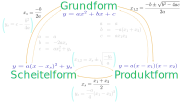
\includegraphics[width=15cm]{allg/funktionen/img/formen/formen.png}
\end{center}

\begin{bemerkung}{}{}
  Das $a$,  ist in allen Formen derselbe Wert und bestimmt die Parabelöffnung.
  \end{bemerkung}
\newpage

\textbf{Grundform aus Scheitelform} (einfaches Ausmultiplizieren). Beispiel:
$$y=2(x-3)^2-4 = 2(x^2-6x+9)-4=2x^2-12x+14$$

\begin{tabular}{rcl}
$a(x-x_S)^2+y_S$ &=& $ax^2-2ax_Sx + (ax_S^2+y_S)$\\
  $a$ &=& $a$ \\
  $b$ &=& $-2ax_S$\\
  $c$ &=& $ax_S^2+y_S$
\end{tabular}


\textbf{Grundform aus Produktform} (einfaches Ausmultiplizieren). Beispiel
$$y=2(x+3)(x-4)=2(x^2 +(3-4)x - 12) = 2x^2-x-24$$

\begin{tabular}{rcl}
  $a(x-x_1)(x-x_2)$ &=& $ax^2 - a(x_1+x_2)x + ax_1x_2$\\
  $a$ &=& $a$ \\
  $b$ &=& $-a(x_1+x_2)$\\
  $c$ &=& $ax_1x_2$
\end{tabular}


\textbf{Nullstellenform (Produktform) aus Grundform}:
Gegeben: $y = ax^2 + bx + c$

Nullstellenform: $y = a(x-x_1)\cdot{}(x-x_2)$ mit

$$x_{1,2} = \frac{-b \pm \sqrt{b^2-4ac}}{2a}$$

\begin{beispiel}{}{}
Gegeben $y = 5x^2 - 5x - 30$. Schreiben Sie dies in der Produktform (=
Nullstellenform):
\platzFuerBerechnungen{3.2}\TRAINER{$y = 5(x-3)(x+2)$\vspace{4.2cm}}
\end{beispiel}
\newpage


\textbf{Scheitelform aus Grundform}:
$$x_S=\frac{-b}{2a}$$

$y_S$ einfach durch Einsetzen von $x_S$ in die Grundform:
$$y_S=c-\frac{b^2}{4a}$$
 
\textbf{Scheitelform aus Produktform}: $x_S$ ist der Mittelwert der beiden
Nullstellen:
$$x_S=\frac{x_1+x_2}{2}$$
Danach $y_S$ einfach durch Einsetzen von $x_S$ in die Produktform:
$$y_S=\frac{-a}{4}(x_1-x_2)^2$$

\textbf{Produktform aus Scheitelform}: Einfachster Weg geht über die Grundform oder abgekürzt:
$$x_{1,2} =x_S \pm \sqrt{\frac{-y_S}{a}}$$


\subsection{Aufgaben}

\TALS{\olatLinkArbeitsblatt{Umrechnen der Formen}{https://olat.bbw.ch/auth/RepositoryEntry/572162090/CourseNode/103176133021102}{1., 2., 3. und 8.}}



\newpage

% Bereits in typ I II und III eingebaut
%\subsection{Parabel aus drei Punkten}
Vorzeigeaufgabe Marthaler Algebra S. 272 Aufg. 3. b) 


\subsection*{Aufgaben}

\AadBMTA{272}{3. a) c)}%% war Marthaler S. 187 Aufg. 676 a) und b)
\GESOAadBMTA{???}{???}

\newpage



%\newpage

%

%%%%%%%%%%%%%%%%%%%%%%%%%%%%%%%%%%%%%%%%%%%%%%%%%%%%%%%%%%%%%%%%
\subsection{Extremwertaufgaben}



\subsubsection{Aus alter Maturprüfung}

\aufgabenFarbe{Gegeben ist die Funktion $f(x) = x\cdot{}(3-\sqrt{x})$,
  $x\in[0;\infty[$.\\
  a) Bestimmen Sie die Nullstellen und das  Extremum der Funktion
  $f$.\\
  b) Im ersten Quadranten, zwischen dem  Graphen und der
  $x$-Achse ist ein  rechtwinkliges Dreieck $ABC$ einbeschrieben.  Der
  rechte Winkel ist in der Ecke $B$.  Punkt $A$ liegt im Ursprung, $B$
  auf der  $x$-Achse und $C$ auf dem Graphen von $f$. Berechnen Sie
  die Koordinaten des  Punktes $C$ so, dass der Flächeninhalt des
  Dreiecks maximal wird.
}%% END aufgabenFarbe

    
\bbwCenterGraphic{8cm}{tals/fct3/img/Maximieren.png}
\TNTeop{
   a) solve$(f(x)=0,x)$ Somit sind die Nullstellen bei 0 und 9\\
     $\text{fmax}(f(x),x)$ liefert $x=4$ ist Maximalstelle (und auch
     Maximalwert ($f(4)=4$)\\
   b) $\text{fmax}(0.5\cdot{}x\cdot{}f(x), x)$ liefert $x = 5.76$ und
   $f(5.76) = 3.456$}%% End TNTeop
\newpage
\subsection*{Aufgaben}
\AadBMTA{311}{49.}
\AadBMTA{321}{17.}

%\newpage

\section{Berührende Graphen}\index{Graphen!berührende}\index{berührende Graphen}

\textbf{Einführungsbeispiel}


Gegeben ist die Parabel $f: y=\frac{1}{4}x^2 -\frac12x +\frac14$ und von einer
Geraden $g$ ist der $y$-Achsenabschnitt $b = -2$ gegeben.

Gesucht ist von der Geraden $g$ die Steigung $a$ so, dass die
Gerade die Parabel tangiert; also genau in einem Punkt berührt.

Wo (in welchem Punkt $B=(x_B|y_B)$) tangiert also die Gerade $g$ die Parabel $f$?

In der folgenden Skizze sind drei mögliche Geraden mit $y$-Achsenabschnitt
$-2$ gezeichnet. Nur eine dieser drei Geraden \textit{tangiert} die Parabel.

\bbwGraph{-4}{4}{-3}{5}{
  \draw[thick,color=blue,variable=\x,domain=-3.5:4] plot ({\x},   {0.25*\x*\x -0.5*\x + 0.25});

  \draw[color=red,variable=\x,domain=-3:5] plot ({\x},{2*\x -2});
  \draw[color=red,variable=\x,domain=-3:5] plot ({\x},{0.5*\x - 2});
  \draw[color=cyan,thick,variable=\x,domain=-3:5] plot ({\x},{1*\x  -2});

  \bbwDot{3, 1}{green}{north}{B}

  %%%\draw[thick,color=blue,variable=\x,domain=-1:5] plot ({\x}, {0.5*\x*\x - 2*\x + 3}); 
  %%\draw[color=red,variable=\x,domain=-1:5] plot ({\x},{0.5*\x + 1});
  %%\draw[color=red,variable=\x,domain=-1:5] plot ({\x},{0.5*\x - 1.5});
  %%\draw[color=cyan,thick,variable=\x,domain=-1:6] plot ({\x},{0.5*\x  -0.125});
  %%\bbwDot{2.5, 1.125}{green}{north}{P}
}
\newpage
\textbf{Lösungsidee}: Der gesuchte Parameter ist $a$, die Steigung der
Geraden.

Nun berechne die Schnittpunkte/den Schnittpunkt mit $$f(x) = g(x).$$

Das $a$ ist gefunden, sobald die Gleichung $f(x)=g(x)$ genau eine
Lösung aufweist; dann also, wenn


\TNT{2}{die Diskriminante dieser Gleichung
verschwindet.}

Den $x$-Wert dieses Berührungspunktes nennen wir $x_B$:


Ansatz:

$$f(x_B) = g(x_B)$$

\TNT{4.4}{
 
\begin{tabular}{rclr}
$\frac14x_s^2-\frac12x_s+\frac14$          & $=$ &  $ax_s-2$ & \\
$\frac14x_s^2+(-\frac12-a)x_s + \frac94$   & $=$ & $0$       & (I)\\
\end{tabular}
\vspace{10mm}
}%% END TNT

Die Diskriminante $D=B^2 - 4AC$ muss gleich 0 sein. 

\TNT{7.2}{
$A = \frac14$, $B = -\frac12-a$ und $C = \frac94$.

  $$D=0=B^2-4AC = (-\frac12-a)^2  - (4\cdot{}A\cdot{}C)$$
  $$0 = (a^2+a+\frac14) - (4\cdot\frac14\cdot{}\frac{+9}4)$$
$$\Longrightarrow 0 = a^2 + a - 2$$
$$\Longrightarrow a_1 = 1 \text{ und  } a_2 = -2$$
\vspace{40mm}
}%% END TNT
\newpage

Für den \textbf{Berührungspunkt} $B=(x_B|y_B)$ müssen wir nun nur doch das gefundene
$a$ in die Gleichung (I) einsetzen.


\TNT{6}{
  $$0 = \frac14x_B^2 + (-\frac12 -a ) + \frac94$$

  $$x_B = x_1 = x_2 = \frac{-B \pm\sqrt{D}}{2A} = \frac{-B \pm
    \sqrt{0}}{2A} = \frac{-B}{2A}$$

  $$x_B = \frac{-B}{2A} = \frac{- (-\frac12 - a)}{\frac24} =
  \frac{\frac12 + a}{\frac12} = (\frac12 + a) : \frac12 = (\frac12+a)
  \cdot{} 2 = 1+2a$$
}



1. Fall: ($a_1=1$):

\TNT{6}{
$B_1: a_1 = 1:$
  $$x_B = 1+2a = 1 + 2\cdot{}(1) = 3$$

Das $y$ finden wir einfach durch Einsetzen von $x$ in den
Funktionsterm der Geradengleichung.

$$y_1 = a_1x_1 - 2 = 1\cdot{}3-2 = 1$$
und somit ist
$$B_1 = (3 | 1)$$
}%% END TNT



2. Fall: ($a_1=-2$):


\TNTeop{
$B_2: a_2 = -2:$
  $$x_B = 1+2a = 1 + 2\cdot{}(-2) = 1-4=-3$$


$$y_2 = a_2x_2+b = -2\cdot{}3-2 = 4$$
und somit ist
$$B_2 = (-3 | 4)$$

}%% END TNT
\newpage




\begin{rezept}{Berührende Graphen}{}

  Bei Berührungsaufgaben mit Parabeln hilft i.\,d.\,R. das folgende
  Vorgehen:

  \begin{enumerate}
  \item Funktionsterme Gleichsetzen: $$f(x) = g(x)$$
  \item In Grundform bringen: $$f(x) - g(x) = 0  \hspace{40mm}
    (I)$$
  \item Diskriminante $D = 0 $ setzen, um den Parameterwert zu
    bestimmen.
  \item Gleichung $(I)$ auflösen mit dem Wissen $D=0$.
    $$x_B=x_1=x_2= \frac{-B}{2A}$$

  \item Gefundenen Parameter in $x_B=\frac{-B}{2A}$ einsetzen, um $x$
    des Berührungspunktes zu bestimmen.
  \item Das $y_B$ des Berührungspunktes ermitteln, indem wir $x_B$ in
    $f$ oder $g$ einsetzen.
    \end{enumerate}
\end{rezept}


\TRAINER{(Je nach Zeit wäre 699. a) noch eine Vorzeigeaufgabe.)}

\subsection{Aufgaben}
\TRAINER{Achtung, dass nicht das Gleichungssystem bereits
  nach dem Gleichsetzen der Graphen aufgestellt wird. Erst nach dem
  Null-Setzen der Diskriminante erhalten wir eine gültige Gleichung
  für das Gleichungssystem.}
%%\TALSAadBMTA{190}{698., 702., 703., 705.}
\TALSAadBMTA{277}{30. a), 36. a), 40. a) c), 42. a), 43. a), 44. a)}
\newpage


\subsection{Grenzwerte und Steigungsfunktion (Optional)}

Wie macht das ein CAS, dass es den tiefsten bzw. den höchsten Punkt
einer Funktion bestimmen kann? Hier ein Erklärungsversuch am Beispiel
der quadratischen Funktion.
Betrachten wir die allgemeine quadratische Funktion $$p: y=ax^2 + bx +
c$$
Mit dem selben $a$ und dem selben $b$ kann ich eine Gerade $s$
definieren, die ich die (Tangenten-)\textbf{Steigungsfunktion}\footnote{Diese
  Steigungsfunktion wird in der Mathematik die
  \textbf{Ableitung}\index{Ableitung} genannt. Genau genommen handelt
  es sich nicht um die Steigung der Parabel, sondern um die Steigung
  einer im Punkt $P=(X_P|f(x_P))$ angelegter Tangente.} nenne:
$$s: y= 2ax+b$$
\newpage


Diese Steigungsfunktion $s$ gibt in jedem Punkt $x$ die Steigung einer
Tangente an die Parabel $p$ an.

\begin{beispiel}{Parabel}{}
  Gegeben ist die Parabel $$p: y=2.5x^2 - 3x + 6.5\text{.}$$

  Wo (für welches $x$) hat diese Parabel
  ihren Tiefpunkt? \TRAINER{Scheitelpunkt:}

  $$x_B =   \LoesungsRaumLen{8cm}{\frac{-b}{2a} = \frac{-(-3)}{2\cdot{}2.5} = 0.6}$$

  Dies ist gleichzeitig die Nullstelle der
  Steigungsfunktion:

  $$s: y= \LoesungsRaumLen{3cm}{2\cdot{}2.5x - 3}$$

  Nullstelle von $s$:

  $$x_0 = \LoesungsRaumLen{7cm}{\frac{3}{2\cdot{}2.5} = 0.6}$$

  Wir können damit aber auch die Steigung in einem ganz anderen Punkt
  \zB für $x=10$ berechnen. Die Parabel $p$ hat an der Stelle $x=10$
  die Tangentensteigung, die durch die Steigungsfunktion im Punkt $10$
  ermittelt wird:

  $$s(10) = \LoesungsRaumLen{40mm}{2\cdot{}10\cdot{2.5} - 3 = 47}$$
  
\end{beispiel}
\newpage

\begin{beispiel}{Gerade gesucht}{}
Gegeben ist die Parabel $$p: y=4x^2 -6x + 3\text{.}$$ Gesucht ist die Gerade
$g: y=ax+b$, sodass die Gerade die Parabel bei $x=7$ berührt.

\begin{enumerate}
\item Die Steigungsfunktion $s$ lautet: $$s:
  y=\LoesungsRaumLen{5cm}{2\cdot{}4x - 6}$$
  
\item Für $x=7$ hat die Steigungsfunktion den Wert \LoesungsRaumLen{1cm}{50}, und somit hat
  die Parabel bei $x=7$ die Steigung \LoesungsRaumLen{1cm}{50}.

  
\item Um den Berührungspunkt $B$ zu finden, setzen wir 7 diesen in $p$
  ein
  $$p(7)= \LoesungsRaumLen{5cm}{4\cdot{}49-6\cdot{}7+3 = 157}$$
  und somit ist
  $$B=(\LoesungsRaum{7}|\LoesungsRaum{157})$$
  
\item Die gesuchte Gerade $g: y=ax+b$ hat also auch die Steigung \LoesungsRaum{50}
  und verläuft durch den Berührungspunkt $B=(\LoesungsRaumLen{9mm}{7}|\LoesungsRaumLen{11mm}{157})$. Also
  $$\LoesungsRaumLen{7cm}{157=50\cdot{}7+b}$$

  Somit ist das gesuchte
  $$b = \LoesungsRaumLen{55mm}{157-50\cdot{}7=-193}$$
  
  und die gesuchte Funktionsgleichung der Geraden lautet: $$y = \LoesungsRaumLen{22mm}{50x-193}$$
  \end{enumerate}
\end{beispiel}

\TRAINER{Idee: Auf mm-Papier eine Funktion $y=\frac1{27}x^3-\frac19
  x^2 - \frac89 x$ vorgeben.

Auftrag: Legen Sie in 5 Punkten eine Tangente an die Funktion und
bestimmen Sie deren Steigung.
Tragen Sie die Steigung in ein neues Koordinatensystem ein: $x$-Achse
= $x$ Wert, $y$-Achse = Steigung der Funktion.
$$f' : y = \frac19 (x-1)^2 - 1 $$
}%%
\newpage

\subsubsection{Beweis der Formel der (Tangenten-)Steigungsfunktion}

Betrachten wir auf auf der $x$-Achse zwei benachbarte Punkte $x$ und
$x+\Delta$. Die Funktionswerte lauten $f(x)$ und $f(x+\Delta)$. Die
\textbf{Steigung} kann nun für eine Gerade bestimmt werden durch:

\bbwCenterGraphic{7cm}{tals/fct3/img/Steigungsfunktion.jpg}

$$\frac{f(x+\Delta) - f(x)}{\Delta}$$

Dies gilt für eine Parabel $p: y=ax^2+bx+c$ näherungsweise auch:
$$\frac{f(x+\Delta)-f(x)}{\Delta} = \frac{(a(x+\Delta)^2 + b(x+\Delta)
  + c) - (ax^2 + bx +c)}{\Delta}=2ax+a\Delta+b$$

Wenn wir nun das $\Delta$ gegen Null gehen lassen, also immer kleinere
Werte einsetzen, so verschwindet der Term $a\cdot{}\Delta$ fast und unsere
Formel stimmt annähernd --- jedoch präzise genug, um dies als Beweis
gelten zu lassen.

Ein anderer Beweis wäre die Tangente effektiv einzusetzen und diese so
zu wählen, dass es genau einen Schnittpunkt gibt, was wieder darauf
zurückführt, dass die Diskriminante = Null gesetzt werden muss. Dann
sind wir exakt, aber der Beweis ist ungleich aufwändiger.
\newpage


\newpage



%% Metapackage Funktionen I
%%%%%%%%%%%%%%%55
%% Funktionen II TALS Metapackage
\part{Funktionen II}\index{Funktionen!II|textbf}
\renewcommand{\bbwPartID}{FCT2}
%%
%% 2019 07 04 Ph. G. Freimann
%%

\section{Quadratische Funktionen}\index{Funktionen!quadratische}
\sectuntertitel{Geraden im Lande der Parabeln wird dringend angeraten, einen
  Integrationskurs zu besuchen.}
%%%%%%%%%%%%%%%%%%%%%%%%%%%%%%%%%%%%%%%%%%%%%%%%%%%%%%%%%%%%%%%%%%%%%%%%%%%%%%%%%

%%\bbwCenterGraphic{8cm}{tals/fct2/img/lugano2018.jpg}
%%\textit{Bildlegende: Parabeln in Lugano (2018)}
\bbwCenterGraphic{175mm}{tals/fct2/img/paris2022.jpg}
\textit{Bildlegende: Parabeln in den Gärten von Versailles (2022)}

\subsection*{Lernziele}

\begin{itemize}
\item Definition
\item Formen: Scheitel-, Produkt-, Normalform
\item Graphische Darstellung
\item Translationen und Spiegelungen
\end{itemize}

\TadBMTA{260}{15}
%%\TALS{(\cite{frommenwiler17alg} S.183 (Kap. 3.4))}
%%\GESO{(\cite{marthaler21alg}       S.260 (Kap. 15))}

Einstieg: Bilder von Heimgartner/Hunziker.


\textbf{Einstiegsaufgabe: } \aufgabenFarbe{Lösen Sie Aufgaben 1. und 2.
  von Seite 272: Welche der angegebenen Funktionen sind quadratisch?}

\newpage

\subsection{Parabel}\index{Parabel}\index{Normalparabel}

Zeichnen Sie die Funktionen $f: y=x^2$ (= Normalparabel), $y=\frac{1}{3}x^2$

und $y=-0.25\cdot{}x^2$  ins Koordinatensystem:

\bbwGraph{-3}{3}{-3}{7}{
  \TRAINER{\bbwFuncC{\x * \x}{-2.5:2.5}{green}
    \bbwFuncC{-0.25*\x * \x}{-3:3}{green}
    \bbwFuncC{\x * \x / 3}{-3:3}{green}
  }
}


\newpage

\subsection{Grundform}\index{Grundform!quadratische Funktion}\index{Quadratische Funktion!Grundform}
Die Funktion $f(x): x \mapsto y = ax^2 + bx +c$ ist eine
quadratische Funktion in Grundform\index{Grundform!quadratische Funktion}.

Spielen Sie mit \TALS{dem TI-nSpire oder mit} \texttt{geogebra.org} an den Parametern $a$, $b$ und $c$ der Funktionsgleichung $y = a\cdot{}x^2 + b\cdot{} x + c$ herum. Was bewirkt der Parameter

$a$: \LoesungsRaumLang{Parabelöffnung: $|a|$ klein: Breite (weite) Öffnung / $|a|$ groß: Enge, schmale Öffnung. $a < 0$: Parabel ist nach unten geöffnet. $a > 0$: Parabel ist nach oben geöffnet.}

$b$: \LoesungsRaumLang{«Parabelsteigung»\footnote{Mit «Parabelsteigung» ist hier die Steigung der entsprechenden Tangente gemeint.} im Punkt $A(0|c)$}

$c$: \LoesungsRaumLang{$y$-Achsenabschnitt. Damit wird eine Verschiebung der Parabel entlang der $y$-Achse erreicht.}

Versuchen Sie eine Parabel mit Scheitelpunkt $(1|1)$ zu finden\TRAINER{(Lösung: $b=-2a$ und $a+b+c=1$.)}.

\subsection*{Aufgaben}
%%\TALSAadBMTA{184ff}{660. a) c) f), 662. a) b) c) und e)}
\AadBMTA{273}{5., 6., 7., 8. und 9.}
\newpage

\subsection{Vier charakteristische Punkte}
Zeichnen Sie die Funktion
$$p: y = x^2 - 4x + \frac{7}{4}$$

\bbwGraph{-3}{6}{-3}{2}{
\TRAINER{\bbwFunc{\x*\x - 4*\x + 1.75}{-0.2:4}}
}%% end BBW Graph

Wo befinden sich die charakteristischen Punkte?

\TNT{2.4}{\vspace{24mm}}


Die charakteristischen Punkte sind:
\begin{itemize}
\item Schnittpunkt mit $y$-Achse = (\LoesungsRaum{0} | \LoesungsRaum{1.75})
\item Nullstellen: $N_1=(\LoesungsRaum{0.5}| \LoesungsRaum{0}), N_2=( \LoesungsRaum{3.5}|\LoesungsRaum{0})$
\item Scheitelpunkt: $S=(\LoesungsRaum{2}|\LoesungsRaum{-2.25})$
\end{itemize}
 
Wie berechnen sich nun diese Punkte?
\newpage
\subsubsection{Parabelöffnung}
Eigentlich ist die Parabelöffnung kein charakteristischer
Punkt. Dennoch kann man eine $x$-Einheit vom Scheitelpunkt entfernt,
das $a$ der Grundform ($y=ax^2+bx+c$) direkt ablesen. Gehen wir bei
der Normalparabel ($a=1$) vom
Scheitelpunkt um eine Einheit nach rechts, so muss die Parabel um eine
$y$-Einheit nach oben anwachsen.

\TNT{10}{
Parabel durch Scheitelpunkt $P=(-3|1)$ und durch $(-2|2)$ =
verschobene Normalparbel zeichnen.

Parabel mit Scheitelpunkt $P=(2|2)$ durch $(3|0.5)$ zeichnen. Das $a$
ist somit sofort $a=-1.5$ abzulesen.
}

\subsubsection{$y$-Achsenabschnitt}
Genau wie bei der linearen Funktion, gilt für den $y$-Achsenabschnitt,
dass die $x$-Koordinate dieses Punktes Null ist.
$$y = x^2 -4x + 1.75$$
wird mit $x=0$ zu
$y = 1.75$.

Der $y$-Achsenabschnitt ist somit immer das $c$ aus $y = ax^2 + bx +
c$.

\newpage

\subsubsection{Nullstellen}
Wie bei den linearen Funktionen sind auch hier die
Nullstellen die Schnittpunkte mit der $x$-Achse. Dies bedeutet für die
Nullstellen $N(x_0 | y_0)$, dass die $y$-Koordinate = 0 ist. Es gilt
also

$$0 = x^2 - 4 x + \frac{7}{4} $$

Dies ist eine quadratische Gleichung mit den Lösungen:

$$x_{1,2} = \frac{-b \pm \sqrt{b^2-4ac}}{2a}$$ 

\noTRAINER{\platzFuerBerechnungen{2.4}}
\TRAINER{$x_{1} = 0.5; x_{2}=3.5$ (Mitternachtsformel)
  \vspace{3cm}}

\begin{bemerkung}{}{}
  Die Nullstellen der quadratischen Funktion entsprechen den Lösungen
  der zugehörigen quadratischen Funktion (mit $y=0$). Daher gilt
  auch hier: 


  \begin{tabular}{c|p{8cm}}
    Diskriminante $D=b^2-4ac$ > 0 & Es gibt zwei Nullstellen. \\
    \hline\\
    Diskriminante $D=b^2-4ac$ = 0 & Es gibt eine Nullstelle, denn der Scheitelpunkt liegt auf der $x$-Achse.\\
    \hline\\
    Diskriminante $D=b^2-4ac$ < 0 & Es gibt keine Nullstellen, denn die Parabel schneidet die $x$-Achse nicht.\\
  \end{tabular}
  
 \ifisALLINONE{Zum Begriff \textbf{Diskriminante}:  \totalref{diskriminante}}\fi{} 
\end{bemerkung}

\subsection*{Aufgaben}
\AadBMTA{277ff}{28. a) c) }

\newpage



\subsubsection{Scheitelpunkt}\index{Scheitelpunkt}
Der Tief- bzw. Hochpunkt einer Parabel wird \textbf{Scheitelpunkt}
genannt.

Wir berechnen den Scheitelpunkt in zwei Schritten.

\textbf{Erstens:} Wir berechnen den Mittelwert der beiden Nullstellen:
$$x_S := \frac{x_{1} + x_{2}}{2} = \frac{\frac{-b+\sqrt{D}}{2a} + \frac{-b-\sqrt{D}}{2a}}{2} =
\frac{(-b+\sqrt{D}) + (-b-\sqrt{D})}{4a} =\frac{-b}{2a}$$
Dabei ist $D$ die Diskriminante $D=b^2-4ac$.

\platzFuerBerechnungen{2.4}
\TRAINER{$x_S = 2$
\vspace{3cm}}

\textbf{Zweitens:} Wir setzen den gefundenen $x$-Wert
(\LoesungsRaum{2}) in die Funktionsgleichung
ein:
$$y_S = x^2 - 4x + 1.75$$
$$y_S = (\LoesungsRaum{2})^2 - 4\cdot{}(\LoesungsRaum{2}) + 1.75$$

Wir erhalten für den Scheitelpunkt $S$: $S=(x_S | y_S) = (\LoesungsRaum{2} | \LoesungsRaum{-2.25})$.

\begin{gesetz}{Scheitelpunkt}{}
  Der Scheitelpunkt $S$ einer Parabel in der Grundform ($y=ax^2+bx+c$) kann wie folgt
  berechnet werden:

  $$S=\left(\frac{-b}{2a}\middle|\frac{4ac-b^2}{4a}\right)$$

  (Bem.: Der $y$-Wert kann einfach durch Einsetzen des $x$-Wertes in
  die Funktionsgleichnug gefunden werden.)
  \end{gesetz}
  
\subsection*{Aufgaben}
%%\TALSAadBMTA{184ff}{665. a) b) c) 666. a) b) c) e) f) g)}
\AadBMTA{273}{4. (=Aufg. 22. S. 276)}

\newpage

\subsection{Bestimmen der Funktionsgleichung}
\TALS{S. 187 Kap. 3.4.3}

\subsubsection{Referenzaufgaben}

\textbf{TYP I}

Gegeben ist ein Punkt $P$ mit den Koordinaten $(2.3 | -1.5)$. Gesucht ist die reinquadratische Funktion $f: y=a\cdot{}x^2$, welche durch diesen Punkt geht.
Machen Sie vorab eine Skizze.

\bbwGraph{-3}{3}{-2}{1}{
  \TRAINER{\bbwFunc{-0.2836 * \x * \x}{-2.5:2.5}
    \bbwDot{2.3,-1.5}{blue}{west}{P}
  }%% end TRAINER
}%% end BBW Graph

\platzFuerBerechnungen{3.6}

\TRAINER{Idee: Punkt einsetzen: $-1.5 = a\cdot{}(2.3)^2$. Das Auf"|lösen dieser Gleichung liefert $a = \frac{-1.5}{2.3^2}$. Dies liefert $a\approx -0.2836$}

Weitere «TYP 1» Aufgaben wären z. B. $y = 3x^2 - bx + 4$ oder $y=2x^2
-7x + c$ mit anderen Worten alle Parabeln mit genau \textbf{einem}
Parameter, daher «Typ 1».

\newpage



\textbf{TYP II}

Gegeben sind zwei Punkte und wir haben zwei Unbekannte.

\begin{rezept}{}{}
  Gesucht sind $a$ und $c$ aus $y = ax^2 + c$ bei den gegebenen
  Punkten $(7|5)$ und $(2|-4)$.

  Wir lösen dies auch durch Einsetzen der Punkte in die
  Funktionsgleichung und wir erhalten zwei Gleichungen:


  \begin{tabular}{c | r  c  r |}
    (I)  &  $5$ & = & $(7)^2\cdot{} a + c$ \\
    (II) & $-4$ & = &  $(2)^2\cdot{} a + c$ \\
  \end{tabular}

  Durch Subtrahieren der Gleichungen erhalten wir

  \begin{tabular}{c | r  c  r | c}
    (I)  &  $5$ & = & $49\cdot{} a + c$ & \,\\
    (II) & $-4$ & = &  $4\cdot{} a + c$ & $\ominus$\\
  \end{tabular}

  $$9 = 45a$$ und somit
  $$a =\frac{1}{5}.$$

  Dieses $a$ (= $\frac{1}{5}$) setzen wir nun in eine der Gleichungen
  (\zB (I)) ein und erhalten
  $$5=49\cdot{}\frac{1}{5} + c$$
  und nach Auf"|lösen erhalten wir $c=\frac{-24}{5}$.

  Die gesuchte Gleichung lautet also:

  $$y = \frac{1}{5}x^2 - \frac{24}{5}$$
\end{rezept}

Probe durch Einsetzen der $x$-Werte der Punkte in die gefundene Funktionsgleichung:

\TNTeop{}
%%\newpage

\begin{beispiel}{}{}
  Anstelle von $a$ und $c$ können natürlich auch $a$ und $b$ gesucht
  sein. Daher eine zweite Aufgabe.

  Gesucht sind $a$ und $b$ aus $y = ax^2 + bx$ bei den gegebenen

  Punkten $(2|-6)$ und $(-3|5)$.

  Wir lösen dies wiederum durch Einsetzen der Punkte in die
  Funktionsgleichung und wir erhalten die beiden Gleichungen, welche
  wir durch das Additionsverfahren lösen können:

  \begin{tabular}{c | r  c  r | c}
    (I)  &  $-6$ & = & $4a + 2b$ & $\cdot{} 3$ \\
    (II) &   $5$ & = & $9a - 3b$ & $\cdot{} 2$ \\
  \end{tabular}

  somit:
  
  \begin{tabular}{c | r  c  r | c}
    (I')  & $-18$ & = & $12a + 6b$ &\, \\
     \,   & \,    & \,&   \,       & $\oplus$\\
    (II') &  $10$ & = & $18a - 6b$ &\, \\
  \end{tabular}

  Nach Addition der Gleichungen erhalten wir

  $$-8 = 30a$$

  was uns zu $a=\frac{-4}{15}$ bringt.

Dieses $a$ können wir nun wieder in eine der beiden Gleichungen
einsetzen (\zB in (I)):

$$-6=4\cdot{}\frac{-4}{15} + 2b$$

Das Auf"|lösen obiger Gleichung liefert nach Kürzen: $b=\frac{-37}{15}$.

Die gesuchte Funktionsgleichung lautet also

$$y = \frac{-4}{15} x^2 - \frac{37}{15} x.$$

\end{beispiel}

Auch bei «Typ II» kann natürlich jede \textbf{zwei}parametrige quadratische
Funktion herhalten, wie \zB $y=-6cx^2 + bx - c$ durch \textbf{zwei}
gegebene Punkte.
\newpage


\textbf{TYP III}: Gegeben sind hier drei Punkte, wir haben aber auch
drei Unbekannte in $y = ax^2 + bx + c$. Die Punkte sind hier
(1|3), (2|3.5) und (-3|11).

Durch Einsetzen der drei Punkte je in die Funktionsgleichung erhalten
wir drei Gleichungen:

\begin{tabular}{c|r c rcrcr|}
  (I)   & 3   & = & $(1)^2\cdot{}a$  &$+$& $(1)\cdot{}b$  &$+$& c \\ 
  (II)  & 3.5 & = & $(2)^2\cdot{}a$  &$+$& $(2)\cdot{}b$  &$+$& c \\ 
  (III) & 11  & = & $(-3)^2\cdot{}a$ &$+$& $(-3)\cdot{}b$ &$+$& c \\ 
\end{tabular}

Vereinfachen:

\begin{tabular}{c|r c rcrcr|}
  (I)   & 3   & = & $a$  &$+$& $b$  &$+$& c \\ 
  (II)  & 3.5 & = & $4a$ &$+$& $2b$ &$+$& c \\ 
  (III) & 11  & = & $9a$ &$-$& $3b$ &$+$& c \\ 
\end{tabular}

Nun finden wir $a$, indem wir zunächst $c$ durch Subtraktion
eliminieren:

\begin{tabular}{l|r c rcr|}
  (IV) = (II) -   (I) & 0.5  & = & $3a$ &$+$& $b$ \\ 
  (V)  = (III) - (II) & 7.5  & = & $5a$ &$-$& $5b$ \\ 
\end{tabular}

Multiplizieren wir nun die Gleichung (IV) mit 5, so erhalten wir

\begin{tabular}{r|r c rcr|}
  5$\cdot{}$(IV)  & 2.5  & = & $15a$ &$+$& $5b$ \\ 
  (V)             & 7.5  & = & $5a$  &$-$& $5b$ \\ 
\end{tabular}

Durch Addition der beiden Gleichungen (IV) und (V) erhalten wir

$10 = 20a$ oder $a = \frac{1}{2}$.

Um $b$ zu finden, setzen wir $a = \frac{1}{2}$ in (V) ein: $7.5 =
5\cdot{}\frac{1}{2} - 5b$.

Auf"|lösen nach $b$ ergibt $b = -1$.

Zu guter Letzt setzen wir $a = \frac{1}{2}$ und $b=-1$ in die
Gleichung (I) ein, um noch $c$ zu erhalten:

$$3 = a + b + c = \frac{1}{2} - 1 + c$$

Somit ist $c=3.5$ und die Funktionsgleichung lautet:

$$y = \frac{1}{2}x^2 - x + 3.5$$


\TALS{\subsection*{Aufgaben}}
%%\TALSAadBMTA{187ff}{676. a) c), 682., 684.}
\AadBMTA{272}{3. a) c), 20. a) c), 21., 22., 24. a), 25. b)}
\newpage


\subsection{Computer Algebra Systeme (CAS)}\index{CAS}
Das eben gezeigte Beispiel wird in der Praxis meist nicht von Hand,
sondern mit einem Computer-Algebra-System, kurz CAS, gelöst:

\paragraph{Aufgabenstellung}
Gegeben sind wieder drei Punkte (1|3), (2|3.5) und (-3|11).
Gesucht ist die Parabel $y = ax^2 + bx + c$, welche durch die drei
Punkte geht.

Dies wird mit dem \tinspire{} wie folgt gelöst:
\begin{itemize}
\item Definiere die Funktionsgleichung mit
  Parametern\footnote{\tinspire Regel: $ax\ne a\cdot{} x$}:\\
  $$f(x) := a\cdot{}x^2 + b\cdot{}x + c$$
\item Definiere das Gleichungssystem:
  $$gls := \left\{ \begin{array}{l}
    f(1) = 3\\
    f(2) = 3.5\\
    f(-3)= 11\\
  \end{array}\right.$$
\item Löse das Gleichungssystem:
  $$solve(gls,\{a, b, c\})$$
\end{itemize}

\subsection*{Aufgaben}
\AadBMTA{272}{3. b) d)}

\newpage

\subsection{Formen der quadratischen Funktion}
\subsubsection{Nullstellenform}\index{Nullstellenform}

Die \textbf{Nullstellenform} wird auch  «faktorisierte Form» oder
«Produktform» genannt.\index{faktorisierte Form}\index{Produktform}

Beachten Sie die folgende quadr. Funktionsgleichung:

$$y = 3.1(x-5)(x+6)$$

Dies ist eine quadratische Funktion in der sogenannten
\textbf{Nullstellenform}, denn die Nullstellen (hier $x_0 = 5$ oder
$x_0 = -6$) können direkt aus der Funktionsgleichung abgelesen werden.
Wenn wir $y=0$ in die Gleichung setzen (Nullstelle),

$$0 = 3.1(x-5)(x+6)$$
so wird die Gleichung genau dann wahr, wenn (mind.) einer der beiden Klammerausdrücke rechts
gleich Null ist. Die Parabelöffnung (hier 3.1) kann dabei beliebig variieren und ist (neben den Nullstellen) der einzige Parameter.

Die Nullstellenform lautet

\begin{gesetz}{}{}

  $$y = a(x-x_1)\cdot{}(x-x_2)$$

  \end{gesetz}

wobei $x_1$ und $x_2$ die Nullstellen der Parabel bezeichnen. 
\newpage


\subsubsection*{Referenzaufgabe zur Nullstellenform}

\noTRAINER{\bbwGraphic{16cm}{tals/fct2/img/BrunnenNullstellenformOhneKoordinatensystem.png}}
\TRAINER{\bbwGraphic{16cm}{tals/fct2/img/BrunnenNullstellenformMitKoordinatensystem.png}}

Ein parabelförmiger Wasserstrahl spritzt ebenerdig aus einem Brunnen und trifft 7m von der Düse entfernt wieder auf dem Boden auf.
Das Wasser steigt also erst gleich hoch an, wie es danach wieder «herunterfällt».
Dabei wird gemessen, dass 1m von der Düse entfernt der Wasserstrahl 84cm über Boden verläuft.
Können Sie aufrecht unter dem Wasserstrahl hindurchgehen?

Tipp: Skizze und  die Parabelgleichung in Nullstellenform aufschreiben. Die Düse ist der Ursprung der Koordinatensystems.\\

\TNT{5.2}{Die Funktionsgleichung lautet $y=a(x-x_1)(x-x2)$.\\
  Mit den Nullstellen $x_1=0$ und $x_2=7$.\\
  Wir setzen den gemessenen Punkt (1|0.84) in die Gleichung ein und erhalten $0.84 = a\cdot{}(1-0)(1-7)$.\\
  Daraus ergibt sich $a=0.84/(-6) = -0.14 $.\\
  Nun setzen wir 3.5 Meter in die Funktionsgleichung $y = -0.14(x-0)(x-7)$ ein: und erhalten $y=-01.4\cdot{}3.5\cdot{}(-3.5) = 1.715m$; das ist die höchste Parabelstelle.}


\subsection*{Aufgaben}%% Nullstellenform
%%\TALSAadBMTA{185}{663, 678., 680.}
\TALSAadBMTA{277}{30. a) b), 31. b)}
\newpage

%%\TRAINER{\, \newpage}
\subsubsection{Scheitelform}\index{Scheitelform!der quadratischen
  Funktion}
Einstieg: Wo hat die Parabel $f: y=3.6(x-4)^2 + 5$ ihren
Scheitelpunkt?

\TNT{4.4}{CAS: bei $x_S = 4$ und $y_S= 5$; völlig irrelevant ist die 3.6.}

Ist eine quadratische Funktion in der Form
\begin{gesetz}{}{}
$$y = a(x-x_S)^2 + y_S$$
\end{gesetz}
gegeben, so sprechen wir von der \textbf{Scheitelform} oder Scheitelpunktsform.
Das liegt daran, dass diese Parabel ihren Scheitelpunkt bei
$(x_S|y_S)$ hat.

Setzen wir für $x$ = $x_S$ in die Funktionsgleichung, so erhalten wir
gerade die $y$-Koordinate des Scheitelpunktes. Je weiter wir uns nun
mit $x$ von $x_S$ wegbewegen, umso größer wird der Term $(x-x_S)^2$
und zwar in egal welcher Richtung wir uns von $x_S$ wegbewegen, die
$y$-Koordinate verhält sich in beiden Fällen symmetrisch.

Prüfen Sie dies mit TI-nSpire oder \texttt{geogebra.org} an der Funktion

$$y = a\cdot{}(x-p)^2 + q$$

Definieren Sie dabei auch den Punkt $S=(p|q)$. Spielen Sie nun mit
$a$, $p$ und $q$. Was bewirken die Änderungen?
\newpage


\subsubsection{Referenzaufgabe Scheitelform}
Von einer Parabel ist der Scheitel $S(2|3)$ gegeben. Ebenfalls ist bekannt, dass die Parabel durch den Punkt $P\left(-\frac{1}{2}\middle|1\right)$ geht.

  Berechnen Sie die Funktionsgleichung in der Grundform $y = ax^2 + bx + c$. Tipp:
  Schreiben Sie die Funktionsgleichung in der Form $y=a(x - x_S)^2 +  y_S$ und setzen anschließend den Punkt $P$ ein.

  \platzFuerBerechnungen{8.0}%%
  \TRAINER{
    Ansatz:
    $$y = a(x-2)^2 + 3$$
    Jetzt $P$ einsetzen:
    $$1 = a(-\frac{1}{2} - 2)^2 + 3 $$
    Nach $a$ auf"|lösen ergibt:
    $$a=-0.32 (=\frac{-2}{2.5^2})$$
    Nun setzen wir $a=-0.32$ in die Funktionsgleichung $y=a(x-2)^2+3$
    ein:
    $$y=-0.32(x-2)^2+3$$
    und quadrieren das Binom, um die geforderte Grundform zu erhalten:
    $$y = -0.32(x^2 - 4x + 4) + 3 = -0.32x^2 + 1.28x + 1.72$$
  }%%end TRAINER%%

  \subsection*{Aufgabe}
  \AadBMTA{277}{29. a) c) e), 32. a), 33.}
%%  \TALSAadBMTA{185}{679. a), 681., 695., 684. a), 700., 694., 686.(*) und  664.}}

\newpage


\subsection{Umrechnungen der Formen}\index{Formen!der quadratischen Funktion}\index{Quadratische Funktion!Formen}

Nochmals die drei Formen im Überblick:


\begin{tabular}{c|l}
  Form & Funktionsgleichung\\
  \hline\\
  Normalform/Grundform & $f: y= ax^2 + bx + c$\\
  \hline\\
  Nullstellenform, faktorisierte Form oder Produktform & $f: y=a(x-x_0)(x-x_1)$\\
  \hline\\
  Scheitelform & $f: y=a(x-x_S)^2+y_S$\\
  \hline%%
\end{tabular}


\subsubsection{Umrechnungen zwischen den Formen}\index{Umrechnungen!quadratische Funktion}\index{Quadratische Funktion!Umrechnungen}

\begin{center}
  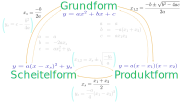
\includegraphics[width=15cm]{allg/funktionen/img/formen/formen.png}
\end{center}

\begin{bemerkung}{}{}
  Das $a$,  ist in allen Formen derselbe Wert und bestimmt die Parabelöffnung.
  \end{bemerkung}
\newpage

\textbf{Grundform aus Scheitelform} (einfaches Ausmultiplizieren). Beispiel:
$$y=2(x-3)^2-4 = 2(x^2-6x+9)-4=2x^2-12x+14$$

\begin{tabular}{rcl}
$a(x-x_S)^2+y_S$ &=& $ax^2-2ax_Sx + (ax_S^2+y_S)$\\
  $a$ &=& $a$ \\
  $b$ &=& $-2ax_S$\\
  $c$ &=& $ax_S^2+y_S$
\end{tabular}


\textbf{Grundform aus Produktform} (einfaches Ausmultiplizieren). Beispiel
$$y=2(x+3)(x-4)=2(x^2 +(3-4)x - 12) = 2x^2-x-24$$

\begin{tabular}{rcl}
  $a(x-x_1)(x-x_2)$ &=& $ax^2 - a(x_1+x_2)x + ax_1x_2$\\
  $a$ &=& $a$ \\
  $b$ &=& $-a(x_1+x_2)$\\
  $c$ &=& $ax_1x_2$
\end{tabular}


\textbf{Nullstellenform (Produktform) aus Grundform}:
Gegeben: $y = ax^2 + bx + c$

Nullstellenform: $y = a(x-x_1)\cdot{}(x-x_2)$ mit

$$x_{1,2} = \frac{-b \pm \sqrt{b^2-4ac}}{2a}$$

\begin{beispiel}{}{}
Gegeben $y = 5x^2 - 5x - 30$. Schreiben Sie dies in der Produktform (=
Nullstellenform):
\platzFuerBerechnungen{3.2}\TRAINER{$y = 5(x-3)(x+2)$\vspace{4.2cm}}
\end{beispiel}
\newpage


\textbf{Scheitelform aus Grundform}:
$$x_S=\frac{-b}{2a}$$

$y_S$ einfach durch Einsetzen von $x_S$ in die Grundform:
$$y_S=c-\frac{b^2}{4a}$$
 
\textbf{Scheitelform aus Produktform}: $x_S$ ist der Mittelwert der beiden
Nullstellen:
$$x_S=\frac{x_1+x_2}{2}$$
Danach $y_S$ einfach durch Einsetzen von $x_S$ in die Produktform:
$$y_S=\frac{-a}{4}(x_1-x_2)^2$$

\textbf{Produktform aus Scheitelform}: Einfachster Weg geht über die Grundform oder abgekürzt:
$$x_{1,2} =x_S \pm \sqrt{\frac{-y_S}{a}}$$


\subsection{Aufgaben}

\TALS{\olatLinkArbeitsblatt{Umrechnen der Formen}{https://olat.bbw.ch/auth/RepositoryEntry/572162090/CourseNode/103176133021102}{1., 2., 3. und 8.}}



\newpage

% Bereits in typ I II und III eingebaut
%\subsection{Parabel aus drei Punkten}
Vorzeigeaufgabe Marthaler Algebra S. 272 Aufg. 3. b) 


\subsection*{Aufgaben}

\AadBMTA{272}{3. a) c)}%% war Marthaler S. 187 Aufg. 676 a) und b)
\GESOAadBMTA{???}{???}

\newpage



%\newpage

%

%%%%%%%%%%%%%%%%%%%%%%%%%%%%%%%%%%%%%%%%%%%%%%%%%%%%%%%%%%%%%%%%
\subsection{Extremwertaufgaben}



\subsubsection{Aus alter Maturprüfung}

\aufgabenFarbe{Gegeben ist die Funktion $f(x) = x\cdot{}(3-\sqrt{x})$,
  $x\in[0;\infty[$.\\
  a) Bestimmen Sie die Nullstellen und das  Extremum der Funktion
  $f$.\\
  b) Im ersten Quadranten, zwischen dem  Graphen und der
  $x$-Achse ist ein  rechtwinkliges Dreieck $ABC$ einbeschrieben.  Der
  rechte Winkel ist in der Ecke $B$.  Punkt $A$ liegt im Ursprung, $B$
  auf der  $x$-Achse und $C$ auf dem Graphen von $f$. Berechnen Sie
  die Koordinaten des  Punktes $C$ so, dass der Flächeninhalt des
  Dreiecks maximal wird.
}%% END aufgabenFarbe

    
\bbwCenterGraphic{8cm}{tals/fct3/img/Maximieren.png}
\TNTeop{
   a) solve$(f(x)=0,x)$ Somit sind die Nullstellen bei 0 und 9\\
     $\text{fmax}(f(x),x)$ liefert $x=4$ ist Maximalstelle (und auch
     Maximalwert ($f(4)=4$)\\
   b) $\text{fmax}(0.5\cdot{}x\cdot{}f(x), x)$ liefert $x = 5.76$ und
   $f(5.76) = 3.456$}%% End TNTeop
\newpage
\subsection*{Aufgaben}
\AadBMTA{311}{49.}
\AadBMTA{321}{17.}

%\newpage

\section{Berührende Graphen}\index{Graphen!berührende}\index{berührende Graphen}

\textbf{Einführungsbeispiel}


Gegeben ist die Parabel $f: y=\frac{1}{4}x^2 -\frac12x +\frac14$ und von einer
Geraden $g$ ist der $y$-Achsenabschnitt $b = -2$ gegeben.

Gesucht ist von der Geraden $g$ die Steigung $a$ so, dass die
Gerade die Parabel tangiert; also genau in einem Punkt berührt.

Wo (in welchem Punkt $B=(x_B|y_B)$) tangiert also die Gerade $g$ die Parabel $f$?

In der folgenden Skizze sind drei mögliche Geraden mit $y$-Achsenabschnitt
$-2$ gezeichnet. Nur eine dieser drei Geraden \textit{tangiert} die Parabel.

\bbwGraph{-4}{4}{-3}{5}{
  \draw[thick,color=blue,variable=\x,domain=-3.5:4] plot ({\x},   {0.25*\x*\x -0.5*\x + 0.25});

  \draw[color=red,variable=\x,domain=-3:5] plot ({\x},{2*\x -2});
  \draw[color=red,variable=\x,domain=-3:5] plot ({\x},{0.5*\x - 2});
  \draw[color=cyan,thick,variable=\x,domain=-3:5] plot ({\x},{1*\x  -2});

  \bbwDot{3, 1}{green}{north}{B}

  %%%\draw[thick,color=blue,variable=\x,domain=-1:5] plot ({\x}, {0.5*\x*\x - 2*\x + 3}); 
  %%\draw[color=red,variable=\x,domain=-1:5] plot ({\x},{0.5*\x + 1});
  %%\draw[color=red,variable=\x,domain=-1:5] plot ({\x},{0.5*\x - 1.5});
  %%\draw[color=cyan,thick,variable=\x,domain=-1:6] plot ({\x},{0.5*\x  -0.125});
  %%\bbwDot{2.5, 1.125}{green}{north}{P}
}
\newpage
\textbf{Lösungsidee}: Der gesuchte Parameter ist $a$, die Steigung der
Geraden.

Nun berechne die Schnittpunkte/den Schnittpunkt mit $$f(x) = g(x).$$

Das $a$ ist gefunden, sobald die Gleichung $f(x)=g(x)$ genau eine
Lösung aufweist; dann also, wenn


\TNT{2}{die Diskriminante dieser Gleichung
verschwindet.}

Den $x$-Wert dieses Berührungspunktes nennen wir $x_B$:


Ansatz:

$$f(x_B) = g(x_B)$$

\TNT{4.4}{
 
\begin{tabular}{rclr}
$\frac14x_s^2-\frac12x_s+\frac14$          & $=$ &  $ax_s-2$ & \\
$\frac14x_s^2+(-\frac12-a)x_s + \frac94$   & $=$ & $0$       & (I)\\
\end{tabular}
\vspace{10mm}
}%% END TNT

Die Diskriminante $D=B^2 - 4AC$ muss gleich 0 sein. 

\TNT{7.2}{
$A = \frac14$, $B = -\frac12-a$ und $C = \frac94$.

  $$D=0=B^2-4AC = (-\frac12-a)^2  - (4\cdot{}A\cdot{}C)$$
  $$0 = (a^2+a+\frac14) - (4\cdot\frac14\cdot{}\frac{+9}4)$$
$$\Longrightarrow 0 = a^2 + a - 2$$
$$\Longrightarrow a_1 = 1 \text{ und  } a_2 = -2$$
\vspace{40mm}
}%% END TNT
\newpage

Für den \textbf{Berührungspunkt} $B=(x_B|y_B)$ müssen wir nun nur doch das gefundene
$a$ in die Gleichung (I) einsetzen.


\TNT{6}{
  $$0 = \frac14x_B^2 + (-\frac12 -a ) + \frac94$$

  $$x_B = x_1 = x_2 = \frac{-B \pm\sqrt{D}}{2A} = \frac{-B \pm
    \sqrt{0}}{2A} = \frac{-B}{2A}$$

  $$x_B = \frac{-B}{2A} = \frac{- (-\frac12 - a)}{\frac24} =
  \frac{\frac12 + a}{\frac12} = (\frac12 + a) : \frac12 = (\frac12+a)
  \cdot{} 2 = 1+2a$$
}



1. Fall: ($a_1=1$):

\TNT{6}{
$B_1: a_1 = 1:$
  $$x_B = 1+2a = 1 + 2\cdot{}(1) = 3$$

Das $y$ finden wir einfach durch Einsetzen von $x$ in den
Funktionsterm der Geradengleichung.

$$y_1 = a_1x_1 - 2 = 1\cdot{}3-2 = 1$$
und somit ist
$$B_1 = (3 | 1)$$
}%% END TNT



2. Fall: ($a_1=-2$):


\TNTeop{
$B_2: a_2 = -2:$
  $$x_B = 1+2a = 1 + 2\cdot{}(-2) = 1-4=-3$$


$$y_2 = a_2x_2+b = -2\cdot{}3-2 = 4$$
und somit ist
$$B_2 = (-3 | 4)$$

}%% END TNT
\newpage




\begin{rezept}{Berührende Graphen}{}

  Bei Berührungsaufgaben mit Parabeln hilft i.\,d.\,R. das folgende
  Vorgehen:

  \begin{enumerate}
  \item Funktionsterme Gleichsetzen: $$f(x) = g(x)$$
  \item In Grundform bringen: $$f(x) - g(x) = 0  \hspace{40mm}
    (I)$$
  \item Diskriminante $D = 0 $ setzen, um den Parameterwert zu
    bestimmen.
  \item Gleichung $(I)$ auflösen mit dem Wissen $D=0$.
    $$x_B=x_1=x_2= \frac{-B}{2A}$$

  \item Gefundenen Parameter in $x_B=\frac{-B}{2A}$ einsetzen, um $x$
    des Berührungspunktes zu bestimmen.
  \item Das $y_B$ des Berührungspunktes ermitteln, indem wir $x_B$ in
    $f$ oder $g$ einsetzen.
    \end{enumerate}
\end{rezept}


\TRAINER{(Je nach Zeit wäre 699. a) noch eine Vorzeigeaufgabe.)}

\subsection{Aufgaben}
\TRAINER{Achtung, dass nicht das Gleichungssystem bereits
  nach dem Gleichsetzen der Graphen aufgestellt wird. Erst nach dem
  Null-Setzen der Diskriminante erhalten wir eine gültige Gleichung
  für das Gleichungssystem.}
%%\TALSAadBMTA{190}{698., 702., 703., 705.}
\TALSAadBMTA{277}{30. a), 36. a), 40. a) c), 42. a), 43. a), 44. a)}
\newpage


\subsection{Grenzwerte und Steigungsfunktion (Optional)}

Wie macht das ein CAS, dass es den tiefsten bzw. den höchsten Punkt
einer Funktion bestimmen kann? Hier ein Erklärungsversuch am Beispiel
der quadratischen Funktion.
Betrachten wir die allgemeine quadratische Funktion $$p: y=ax^2 + bx +
c$$
Mit dem selben $a$ und dem selben $b$ kann ich eine Gerade $s$
definieren, die ich die (Tangenten-)\textbf{Steigungsfunktion}\footnote{Diese
  Steigungsfunktion wird in der Mathematik die
  \textbf{Ableitung}\index{Ableitung} genannt. Genau genommen handelt
  es sich nicht um die Steigung der Parabel, sondern um die Steigung
  einer im Punkt $P=(X_P|f(x_P))$ angelegter Tangente.} nenne:
$$s: y= 2ax+b$$
\newpage


Diese Steigungsfunktion $s$ gibt in jedem Punkt $x$ die Steigung einer
Tangente an die Parabel $p$ an.

\begin{beispiel}{Parabel}{}
  Gegeben ist die Parabel $$p: y=2.5x^2 - 3x + 6.5\text{.}$$

  Wo (für welches $x$) hat diese Parabel
  ihren Tiefpunkt? \TRAINER{Scheitelpunkt:}

  $$x_B =   \LoesungsRaumLen{8cm}{\frac{-b}{2a} = \frac{-(-3)}{2\cdot{}2.5} = 0.6}$$

  Dies ist gleichzeitig die Nullstelle der
  Steigungsfunktion:

  $$s: y= \LoesungsRaumLen{3cm}{2\cdot{}2.5x - 3}$$

  Nullstelle von $s$:

  $$x_0 = \LoesungsRaumLen{7cm}{\frac{3}{2\cdot{}2.5} = 0.6}$$

  Wir können damit aber auch die Steigung in einem ganz anderen Punkt
  \zB für $x=10$ berechnen. Die Parabel $p$ hat an der Stelle $x=10$
  die Tangentensteigung, die durch die Steigungsfunktion im Punkt $10$
  ermittelt wird:

  $$s(10) = \LoesungsRaumLen{40mm}{2\cdot{}10\cdot{2.5} - 3 = 47}$$
  
\end{beispiel}
\newpage

\begin{beispiel}{Gerade gesucht}{}
Gegeben ist die Parabel $$p: y=4x^2 -6x + 3\text{.}$$ Gesucht ist die Gerade
$g: y=ax+b$, sodass die Gerade die Parabel bei $x=7$ berührt.

\begin{enumerate}
\item Die Steigungsfunktion $s$ lautet: $$s:
  y=\LoesungsRaumLen{5cm}{2\cdot{}4x - 6}$$
  
\item Für $x=7$ hat die Steigungsfunktion den Wert \LoesungsRaumLen{1cm}{50}, und somit hat
  die Parabel bei $x=7$ die Steigung \LoesungsRaumLen{1cm}{50}.

  
\item Um den Berührungspunkt $B$ zu finden, setzen wir 7 diesen in $p$
  ein
  $$p(7)= \LoesungsRaumLen{5cm}{4\cdot{}49-6\cdot{}7+3 = 157}$$
  und somit ist
  $$B=(\LoesungsRaum{7}|\LoesungsRaum{157})$$
  
\item Die gesuchte Gerade $g: y=ax+b$ hat also auch die Steigung \LoesungsRaum{50}
  und verläuft durch den Berührungspunkt $B=(\LoesungsRaumLen{9mm}{7}|\LoesungsRaumLen{11mm}{157})$. Also
  $$\LoesungsRaumLen{7cm}{157=50\cdot{}7+b}$$

  Somit ist das gesuchte
  $$b = \LoesungsRaumLen{55mm}{157-50\cdot{}7=-193}$$
  
  und die gesuchte Funktionsgleichung der Geraden lautet: $$y = \LoesungsRaumLen{22mm}{50x-193}$$
  \end{enumerate}
\end{beispiel}

\TRAINER{Idee: Auf mm-Papier eine Funktion $y=\frac1{27}x^3-\frac19
  x^2 - \frac89 x$ vorgeben.

Auftrag: Legen Sie in 5 Punkten eine Tangente an die Funktion und
bestimmen Sie deren Steigung.
Tragen Sie die Steigung in ein neues Koordinatensystem ein: $x$-Achse
= $x$ Wert, $y$-Achse = Steigung der Funktion.
$$f' : y = \frac19 (x-1)^2 - 1 $$
}%%
\newpage

\subsubsection{Beweis der Formel der (Tangenten-)Steigungsfunktion}

Betrachten wir auf auf der $x$-Achse zwei benachbarte Punkte $x$ und
$x+\Delta$. Die Funktionswerte lauten $f(x)$ und $f(x+\Delta)$. Die
\textbf{Steigung} kann nun für eine Gerade bestimmt werden durch:

\bbwCenterGraphic{7cm}{tals/fct3/img/Steigungsfunktion.jpg}

$$\frac{f(x+\Delta) - f(x)}{\Delta}$$

Dies gilt für eine Parabel $p: y=ax^2+bx+c$ näherungsweise auch:
$$\frac{f(x+\Delta)-f(x)}{\Delta} = \frac{(a(x+\Delta)^2 + b(x+\Delta)
  + c) - (ax^2 + bx +c)}{\Delta}=2ax+a\Delta+b$$

Wenn wir nun das $\Delta$ gegen Null gehen lassen, also immer kleinere
Werte einsetzen, so verschwindet der Term $a\cdot{}\Delta$ fast und unsere
Formel stimmt annähernd --- jedoch präzise genug, um dies als Beweis
gelten zu lassen.

Ein anderer Beweis wäre die Tangente effektiv einzusetzen und diese so
zu wählen, dass es genau einen Schnittpunkt gibt, was wieder darauf
zurückführt, dass die Diskriminante = Null gesetzt werden muss. Dann
sind wir exakt, aber der Beweis ist ungleich aufwändiger.
\newpage


\newpage



%% All TALS
%%%%%%%%%%%%%%%55
%% Funktionen II TALS Metapackage
\part{Funktionen II}\index{Funktionen!II|textbf}
\renewcommand{\bbwPartID}{FCT2}
%%
%% 2019 07 04 Ph. G. Freimann
%%

\section{Quadratische Funktionen}\index{Funktionen!quadratische}
\sectuntertitel{Geraden im Lande der Parabeln wird dringend angeraten, einen
  Integrationskurs zu besuchen.}
%%%%%%%%%%%%%%%%%%%%%%%%%%%%%%%%%%%%%%%%%%%%%%%%%%%%%%%%%%%%%%%%%%%%%%%%%%%%%%%%%

%%\bbwCenterGraphic{8cm}{tals/fct2/img/lugano2018.jpg}
%%\textit{Bildlegende: Parabeln in Lugano (2018)}
\bbwCenterGraphic{175mm}{tals/fct2/img/paris2022.jpg}
\textit{Bildlegende: Parabeln in den Gärten von Versailles (2022)}

\subsection*{Lernziele}

\begin{itemize}
\item Definition
\item Formen: Scheitel-, Produkt-, Normalform
\item Graphische Darstellung
\item Translationen und Spiegelungen
\end{itemize}

\TadBMTA{260}{15}
%%\TALS{(\cite{frommenwiler17alg} S.183 (Kap. 3.4))}
%%\GESO{(\cite{marthaler21alg}       S.260 (Kap. 15))}

Einstieg: Bilder von Heimgartner/Hunziker.


\textbf{Einstiegsaufgabe: } \aufgabenFarbe{Lösen Sie Aufgaben 1. und 2.
  von Seite 272: Welche der angegebenen Funktionen sind quadratisch?}

\newpage

\subsection{Parabel}\index{Parabel}\index{Normalparabel}

Zeichnen Sie die Funktionen $f: y=x^2$ (= Normalparabel), $y=\frac{1}{3}x^2$

und $y=-0.25\cdot{}x^2$  ins Koordinatensystem:

\bbwGraph{-3}{3}{-3}{7}{
  \TRAINER{\bbwFuncC{\x * \x}{-2.5:2.5}{green}
    \bbwFuncC{-0.25*\x * \x}{-3:3}{green}
    \bbwFuncC{\x * \x / 3}{-3:3}{green}
  }
}


\newpage

\subsection{Grundform}\index{Grundform!quadratische Funktion}\index{Quadratische Funktion!Grundform}
Die Funktion $f(x): x \mapsto y = ax^2 + bx +c$ ist eine
quadratische Funktion in Grundform\index{Grundform!quadratische Funktion}.

Spielen Sie mit \TALS{dem TI-nSpire oder mit} \texttt{geogebra.org} an den Parametern $a$, $b$ und $c$ der Funktionsgleichung $y = a\cdot{}x^2 + b\cdot{} x + c$ herum. Was bewirkt der Parameter

$a$: \LoesungsRaumLang{Parabelöffnung: $|a|$ klein: Breite (weite) Öffnung / $|a|$ groß: Enge, schmale Öffnung. $a < 0$: Parabel ist nach unten geöffnet. $a > 0$: Parabel ist nach oben geöffnet.}

$b$: \LoesungsRaumLang{«Parabelsteigung»\footnote{Mit «Parabelsteigung» ist hier die Steigung der entsprechenden Tangente gemeint.} im Punkt $A(0|c)$}

$c$: \LoesungsRaumLang{$y$-Achsenabschnitt. Damit wird eine Verschiebung der Parabel entlang der $y$-Achse erreicht.}

Versuchen Sie eine Parabel mit Scheitelpunkt $(1|1)$ zu finden\TRAINER{(Lösung: $b=-2a$ und $a+b+c=1$.)}.

\subsection*{Aufgaben}
%%\TALSAadBMTA{184ff}{660. a) c) f), 662. a) b) c) und e)}
\AadBMTA{273}{5., 6., 7., 8. und 9.}
\newpage

\subsection{Vier charakteristische Punkte}
Zeichnen Sie die Funktion
$$p: y = x^2 - 4x + \frac{7}{4}$$

\bbwGraph{-3}{6}{-3}{2}{
\TRAINER{\bbwFunc{\x*\x - 4*\x + 1.75}{-0.2:4}}
}%% end BBW Graph

Wo befinden sich die charakteristischen Punkte?

\TNT{2.4}{\vspace{24mm}}


Die charakteristischen Punkte sind:
\begin{itemize}
\item Schnittpunkt mit $y$-Achse = (\LoesungsRaum{0} | \LoesungsRaum{1.75})
\item Nullstellen: $N_1=(\LoesungsRaum{0.5}| \LoesungsRaum{0}), N_2=( \LoesungsRaum{3.5}|\LoesungsRaum{0})$
\item Scheitelpunkt: $S=(\LoesungsRaum{2}|\LoesungsRaum{-2.25})$
\end{itemize}
 
Wie berechnen sich nun diese Punkte?
\newpage
\subsubsection{Parabelöffnung}
Eigentlich ist die Parabelöffnung kein charakteristischer
Punkt. Dennoch kann man eine $x$-Einheit vom Scheitelpunkt entfernt,
das $a$ der Grundform ($y=ax^2+bx+c$) direkt ablesen. Gehen wir bei
der Normalparabel ($a=1$) vom
Scheitelpunkt um eine Einheit nach rechts, so muss die Parabel um eine
$y$-Einheit nach oben anwachsen.

\TNT{10}{
Parabel durch Scheitelpunkt $P=(-3|1)$ und durch $(-2|2)$ =
verschobene Normalparbel zeichnen.

Parabel mit Scheitelpunkt $P=(2|2)$ durch $(3|0.5)$ zeichnen. Das $a$
ist somit sofort $a=-1.5$ abzulesen.
}

\subsubsection{$y$-Achsenabschnitt}
Genau wie bei der linearen Funktion, gilt für den $y$-Achsenabschnitt,
dass die $x$-Koordinate dieses Punktes Null ist.
$$y = x^2 -4x + 1.75$$
wird mit $x=0$ zu
$y = 1.75$.

Der $y$-Achsenabschnitt ist somit immer das $c$ aus $y = ax^2 + bx +
c$.

\newpage

\subsubsection{Nullstellen}
Wie bei den linearen Funktionen sind auch hier die
Nullstellen die Schnittpunkte mit der $x$-Achse. Dies bedeutet für die
Nullstellen $N(x_0 | y_0)$, dass die $y$-Koordinate = 0 ist. Es gilt
also

$$0 = x^2 - 4 x + \frac{7}{4} $$

Dies ist eine quadratische Gleichung mit den Lösungen:

$$x_{1,2} = \frac{-b \pm \sqrt{b^2-4ac}}{2a}$$ 

\noTRAINER{\platzFuerBerechnungen{2.4}}
\TRAINER{$x_{1} = 0.5; x_{2}=3.5$ (Mitternachtsformel)
  \vspace{3cm}}

\begin{bemerkung}{}{}
  Die Nullstellen der quadratischen Funktion entsprechen den Lösungen
  der zugehörigen quadratischen Funktion (mit $y=0$). Daher gilt
  auch hier: 


  \begin{tabular}{c|p{8cm}}
    Diskriminante $D=b^2-4ac$ > 0 & Es gibt zwei Nullstellen. \\
    \hline\\
    Diskriminante $D=b^2-4ac$ = 0 & Es gibt eine Nullstelle, denn der Scheitelpunkt liegt auf der $x$-Achse.\\
    \hline\\
    Diskriminante $D=b^2-4ac$ < 0 & Es gibt keine Nullstellen, denn die Parabel schneidet die $x$-Achse nicht.\\
  \end{tabular}
  
 \ifisALLINONE{Zum Begriff \textbf{Diskriminante}:  \totalref{diskriminante}}\fi{} 
\end{bemerkung}

\subsection*{Aufgaben}
\AadBMTA{277ff}{28. a) c) }

\newpage



\subsubsection{Scheitelpunkt}\index{Scheitelpunkt}
Der Tief- bzw. Hochpunkt einer Parabel wird \textbf{Scheitelpunkt}
genannt.

Wir berechnen den Scheitelpunkt in zwei Schritten.

\textbf{Erstens:} Wir berechnen den Mittelwert der beiden Nullstellen:
$$x_S := \frac{x_{1} + x_{2}}{2} = \frac{\frac{-b+\sqrt{D}}{2a} + \frac{-b-\sqrt{D}}{2a}}{2} =
\frac{(-b+\sqrt{D}) + (-b-\sqrt{D})}{4a} =\frac{-b}{2a}$$
Dabei ist $D$ die Diskriminante $D=b^2-4ac$.

\platzFuerBerechnungen{2.4}
\TRAINER{$x_S = 2$
\vspace{3cm}}

\textbf{Zweitens:} Wir setzen den gefundenen $x$-Wert
(\LoesungsRaum{2}) in die Funktionsgleichung
ein:
$$y_S = x^2 - 4x + 1.75$$
$$y_S = (\LoesungsRaum{2})^2 - 4\cdot{}(\LoesungsRaum{2}) + 1.75$$

Wir erhalten für den Scheitelpunkt $S$: $S=(x_S | y_S) = (\LoesungsRaum{2} | \LoesungsRaum{-2.25})$.

\begin{gesetz}{Scheitelpunkt}{}
  Der Scheitelpunkt $S$ einer Parabel in der Grundform ($y=ax^2+bx+c$) kann wie folgt
  berechnet werden:

  $$S=\left(\frac{-b}{2a}\middle|\frac{4ac-b^2}{4a}\right)$$

  (Bem.: Der $y$-Wert kann einfach durch Einsetzen des $x$-Wertes in
  die Funktionsgleichnug gefunden werden.)
  \end{gesetz}
  
\subsection*{Aufgaben}
%%\TALSAadBMTA{184ff}{665. a) b) c) 666. a) b) c) e) f) g)}
\AadBMTA{273}{4. (=Aufg. 22. S. 276)}

\newpage

\subsection{Bestimmen der Funktionsgleichung}
\TALS{S. 187 Kap. 3.4.3}

\subsubsection{Referenzaufgaben}

\textbf{TYP I}

Gegeben ist ein Punkt $P$ mit den Koordinaten $(2.3 | -1.5)$. Gesucht ist die reinquadratische Funktion $f: y=a\cdot{}x^2$, welche durch diesen Punkt geht.
Machen Sie vorab eine Skizze.

\bbwGraph{-3}{3}{-2}{1}{
  \TRAINER{\bbwFunc{-0.2836 * \x * \x}{-2.5:2.5}
    \bbwDot{2.3,-1.5}{blue}{west}{P}
  }%% end TRAINER
}%% end BBW Graph

\platzFuerBerechnungen{3.6}

\TRAINER{Idee: Punkt einsetzen: $-1.5 = a\cdot{}(2.3)^2$. Das Auf"|lösen dieser Gleichung liefert $a = \frac{-1.5}{2.3^2}$. Dies liefert $a\approx -0.2836$}

Weitere «TYP 1» Aufgaben wären z. B. $y = 3x^2 - bx + 4$ oder $y=2x^2
-7x + c$ mit anderen Worten alle Parabeln mit genau \textbf{einem}
Parameter, daher «Typ 1».

\newpage



\textbf{TYP II}

Gegeben sind zwei Punkte und wir haben zwei Unbekannte.

\begin{rezept}{}{}
  Gesucht sind $a$ und $c$ aus $y = ax^2 + c$ bei den gegebenen
  Punkten $(7|5)$ und $(2|-4)$.

  Wir lösen dies auch durch Einsetzen der Punkte in die
  Funktionsgleichung und wir erhalten zwei Gleichungen:


  \begin{tabular}{c | r  c  r |}
    (I)  &  $5$ & = & $(7)^2\cdot{} a + c$ \\
    (II) & $-4$ & = &  $(2)^2\cdot{} a + c$ \\
  \end{tabular}

  Durch Subtrahieren der Gleichungen erhalten wir

  \begin{tabular}{c | r  c  r | c}
    (I)  &  $5$ & = & $49\cdot{} a + c$ & \,\\
    (II) & $-4$ & = &  $4\cdot{} a + c$ & $\ominus$\\
  \end{tabular}

  $$9 = 45a$$ und somit
  $$a =\frac{1}{5}.$$

  Dieses $a$ (= $\frac{1}{5}$) setzen wir nun in eine der Gleichungen
  (\zB (I)) ein und erhalten
  $$5=49\cdot{}\frac{1}{5} + c$$
  und nach Auf"|lösen erhalten wir $c=\frac{-24}{5}$.

  Die gesuchte Gleichung lautet also:

  $$y = \frac{1}{5}x^2 - \frac{24}{5}$$
\end{rezept}

Probe durch Einsetzen der $x$-Werte der Punkte in die gefundene Funktionsgleichung:

\TNTeop{}
%%\newpage

\begin{beispiel}{}{}
  Anstelle von $a$ und $c$ können natürlich auch $a$ und $b$ gesucht
  sein. Daher eine zweite Aufgabe.

  Gesucht sind $a$ und $b$ aus $y = ax^2 + bx$ bei den gegebenen

  Punkten $(2|-6)$ und $(-3|5)$.

  Wir lösen dies wiederum durch Einsetzen der Punkte in die
  Funktionsgleichung und wir erhalten die beiden Gleichungen, welche
  wir durch das Additionsverfahren lösen können:

  \begin{tabular}{c | r  c  r | c}
    (I)  &  $-6$ & = & $4a + 2b$ & $\cdot{} 3$ \\
    (II) &   $5$ & = & $9a - 3b$ & $\cdot{} 2$ \\
  \end{tabular}

  somit:
  
  \begin{tabular}{c | r  c  r | c}
    (I')  & $-18$ & = & $12a + 6b$ &\, \\
     \,   & \,    & \,&   \,       & $\oplus$\\
    (II') &  $10$ & = & $18a - 6b$ &\, \\
  \end{tabular}

  Nach Addition der Gleichungen erhalten wir

  $$-8 = 30a$$

  was uns zu $a=\frac{-4}{15}$ bringt.

Dieses $a$ können wir nun wieder in eine der beiden Gleichungen
einsetzen (\zB in (I)):

$$-6=4\cdot{}\frac{-4}{15} + 2b$$

Das Auf"|lösen obiger Gleichung liefert nach Kürzen: $b=\frac{-37}{15}$.

Die gesuchte Funktionsgleichung lautet also

$$y = \frac{-4}{15} x^2 - \frac{37}{15} x.$$

\end{beispiel}

Auch bei «Typ II» kann natürlich jede \textbf{zwei}parametrige quadratische
Funktion herhalten, wie \zB $y=-6cx^2 + bx - c$ durch \textbf{zwei}
gegebene Punkte.
\newpage


\textbf{TYP III}: Gegeben sind hier drei Punkte, wir haben aber auch
drei Unbekannte in $y = ax^2 + bx + c$. Die Punkte sind hier
(1|3), (2|3.5) und (-3|11).

Durch Einsetzen der drei Punkte je in die Funktionsgleichung erhalten
wir drei Gleichungen:

\begin{tabular}{c|r c rcrcr|}
  (I)   & 3   & = & $(1)^2\cdot{}a$  &$+$& $(1)\cdot{}b$  &$+$& c \\ 
  (II)  & 3.5 & = & $(2)^2\cdot{}a$  &$+$& $(2)\cdot{}b$  &$+$& c \\ 
  (III) & 11  & = & $(-3)^2\cdot{}a$ &$+$& $(-3)\cdot{}b$ &$+$& c \\ 
\end{tabular}

Vereinfachen:

\begin{tabular}{c|r c rcrcr|}
  (I)   & 3   & = & $a$  &$+$& $b$  &$+$& c \\ 
  (II)  & 3.5 & = & $4a$ &$+$& $2b$ &$+$& c \\ 
  (III) & 11  & = & $9a$ &$-$& $3b$ &$+$& c \\ 
\end{tabular}

Nun finden wir $a$, indem wir zunächst $c$ durch Subtraktion
eliminieren:

\begin{tabular}{l|r c rcr|}
  (IV) = (II) -   (I) & 0.5  & = & $3a$ &$+$& $b$ \\ 
  (V)  = (III) - (II) & 7.5  & = & $5a$ &$-$& $5b$ \\ 
\end{tabular}

Multiplizieren wir nun die Gleichung (IV) mit 5, so erhalten wir

\begin{tabular}{r|r c rcr|}
  5$\cdot{}$(IV)  & 2.5  & = & $15a$ &$+$& $5b$ \\ 
  (V)             & 7.5  & = & $5a$  &$-$& $5b$ \\ 
\end{tabular}

Durch Addition der beiden Gleichungen (IV) und (V) erhalten wir

$10 = 20a$ oder $a = \frac{1}{2}$.

Um $b$ zu finden, setzen wir $a = \frac{1}{2}$ in (V) ein: $7.5 =
5\cdot{}\frac{1}{2} - 5b$.

Auf"|lösen nach $b$ ergibt $b = -1$.

Zu guter Letzt setzen wir $a = \frac{1}{2}$ und $b=-1$ in die
Gleichung (I) ein, um noch $c$ zu erhalten:

$$3 = a + b + c = \frac{1}{2} - 1 + c$$

Somit ist $c=3.5$ und die Funktionsgleichung lautet:

$$y = \frac{1}{2}x^2 - x + 3.5$$


\TALS{\subsection*{Aufgaben}}
%%\TALSAadBMTA{187ff}{676. a) c), 682., 684.}
\AadBMTA{272}{3. a) c), 20. a) c), 21., 22., 24. a), 25. b)}
\newpage


\subsection{Computer Algebra Systeme (CAS)}\index{CAS}
Das eben gezeigte Beispiel wird in der Praxis meist nicht von Hand,
sondern mit einem Computer-Algebra-System, kurz CAS, gelöst:

\paragraph{Aufgabenstellung}
Gegeben sind wieder drei Punkte (1|3), (2|3.5) und (-3|11).
Gesucht ist die Parabel $y = ax^2 + bx + c$, welche durch die drei
Punkte geht.

Dies wird mit dem \tinspire{} wie folgt gelöst:
\begin{itemize}
\item Definiere die Funktionsgleichung mit
  Parametern\footnote{\tinspire Regel: $ax\ne a\cdot{} x$}:\\
  $$f(x) := a\cdot{}x^2 + b\cdot{}x + c$$
\item Definiere das Gleichungssystem:
  $$gls := \left\{ \begin{array}{l}
    f(1) = 3\\
    f(2) = 3.5\\
    f(-3)= 11\\
  \end{array}\right.$$
\item Löse das Gleichungssystem:
  $$solve(gls,\{a, b, c\})$$
\end{itemize}

\subsection*{Aufgaben}
\AadBMTA{272}{3. b) d)}

\newpage

\subsection{Formen der quadratischen Funktion}
\subsubsection{Nullstellenform}\index{Nullstellenform}

Die \textbf{Nullstellenform} wird auch  «faktorisierte Form» oder
«Produktform» genannt.\index{faktorisierte Form}\index{Produktform}

Beachten Sie die folgende quadr. Funktionsgleichung:

$$y = 3.1(x-5)(x+6)$$

Dies ist eine quadratische Funktion in der sogenannten
\textbf{Nullstellenform}, denn die Nullstellen (hier $x_0 = 5$ oder
$x_0 = -6$) können direkt aus der Funktionsgleichung abgelesen werden.
Wenn wir $y=0$ in die Gleichung setzen (Nullstelle),

$$0 = 3.1(x-5)(x+6)$$
so wird die Gleichung genau dann wahr, wenn (mind.) einer der beiden Klammerausdrücke rechts
gleich Null ist. Die Parabelöffnung (hier 3.1) kann dabei beliebig variieren und ist (neben den Nullstellen) der einzige Parameter.

Die Nullstellenform lautet

\begin{gesetz}{}{}

  $$y = a(x-x_1)\cdot{}(x-x_2)$$

  \end{gesetz}

wobei $x_1$ und $x_2$ die Nullstellen der Parabel bezeichnen. 
\newpage


\subsubsection*{Referenzaufgabe zur Nullstellenform}

\noTRAINER{\bbwGraphic{16cm}{tals/fct2/img/BrunnenNullstellenformOhneKoordinatensystem.png}}
\TRAINER{\bbwGraphic{16cm}{tals/fct2/img/BrunnenNullstellenformMitKoordinatensystem.png}}

Ein parabelförmiger Wasserstrahl spritzt ebenerdig aus einem Brunnen und trifft 7m von der Düse entfernt wieder auf dem Boden auf.
Das Wasser steigt also erst gleich hoch an, wie es danach wieder «herunterfällt».
Dabei wird gemessen, dass 1m von der Düse entfernt der Wasserstrahl 84cm über Boden verläuft.
Können Sie aufrecht unter dem Wasserstrahl hindurchgehen?

Tipp: Skizze und  die Parabelgleichung in Nullstellenform aufschreiben. Die Düse ist der Ursprung der Koordinatensystems.\\

\TNT{5.2}{Die Funktionsgleichung lautet $y=a(x-x_1)(x-x2)$.\\
  Mit den Nullstellen $x_1=0$ und $x_2=7$.\\
  Wir setzen den gemessenen Punkt (1|0.84) in die Gleichung ein und erhalten $0.84 = a\cdot{}(1-0)(1-7)$.\\
  Daraus ergibt sich $a=0.84/(-6) = -0.14 $.\\
  Nun setzen wir 3.5 Meter in die Funktionsgleichung $y = -0.14(x-0)(x-7)$ ein: und erhalten $y=-01.4\cdot{}3.5\cdot{}(-3.5) = 1.715m$; das ist die höchste Parabelstelle.}


\subsection*{Aufgaben}%% Nullstellenform
%%\TALSAadBMTA{185}{663, 678., 680.}
\TALSAadBMTA{277}{30. a) b), 31. b)}
\newpage

%%\TRAINER{\, \newpage}
\subsubsection{Scheitelform}\index{Scheitelform!der quadratischen
  Funktion}
Einstieg: Wo hat die Parabel $f: y=3.6(x-4)^2 + 5$ ihren
Scheitelpunkt?

\TNT{4.4}{CAS: bei $x_S = 4$ und $y_S= 5$; völlig irrelevant ist die 3.6.}

Ist eine quadratische Funktion in der Form
\begin{gesetz}{}{}
$$y = a(x-x_S)^2 + y_S$$
\end{gesetz}
gegeben, so sprechen wir von der \textbf{Scheitelform} oder Scheitelpunktsform.
Das liegt daran, dass diese Parabel ihren Scheitelpunkt bei
$(x_S|y_S)$ hat.

Setzen wir für $x$ = $x_S$ in die Funktionsgleichung, so erhalten wir
gerade die $y$-Koordinate des Scheitelpunktes. Je weiter wir uns nun
mit $x$ von $x_S$ wegbewegen, umso größer wird der Term $(x-x_S)^2$
und zwar in egal welcher Richtung wir uns von $x_S$ wegbewegen, die
$y$-Koordinate verhält sich in beiden Fällen symmetrisch.

Prüfen Sie dies mit TI-nSpire oder \texttt{geogebra.org} an der Funktion

$$y = a\cdot{}(x-p)^2 + q$$

Definieren Sie dabei auch den Punkt $S=(p|q)$. Spielen Sie nun mit
$a$, $p$ und $q$. Was bewirken die Änderungen?
\newpage


\subsubsection{Referenzaufgabe Scheitelform}
Von einer Parabel ist der Scheitel $S(2|3)$ gegeben. Ebenfalls ist bekannt, dass die Parabel durch den Punkt $P\left(-\frac{1}{2}\middle|1\right)$ geht.

  Berechnen Sie die Funktionsgleichung in der Grundform $y = ax^2 + bx + c$. Tipp:
  Schreiben Sie die Funktionsgleichung in der Form $y=a(x - x_S)^2 +  y_S$ und setzen anschließend den Punkt $P$ ein.

  \platzFuerBerechnungen{8.0}%%
  \TRAINER{
    Ansatz:
    $$y = a(x-2)^2 + 3$$
    Jetzt $P$ einsetzen:
    $$1 = a(-\frac{1}{2} - 2)^2 + 3 $$
    Nach $a$ auf"|lösen ergibt:
    $$a=-0.32 (=\frac{-2}{2.5^2})$$
    Nun setzen wir $a=-0.32$ in die Funktionsgleichung $y=a(x-2)^2+3$
    ein:
    $$y=-0.32(x-2)^2+3$$
    und quadrieren das Binom, um die geforderte Grundform zu erhalten:
    $$y = -0.32(x^2 - 4x + 4) + 3 = -0.32x^2 + 1.28x + 1.72$$
  }%%end TRAINER%%

  \subsection*{Aufgabe}
  \AadBMTA{277}{29. a) c) e), 32. a), 33.}
%%  \TALSAadBMTA{185}{679. a), 681., 695., 684. a), 700., 694., 686.(*) und  664.}}

\newpage


\subsection{Umrechnungen der Formen}\index{Formen!der quadratischen Funktion}\index{Quadratische Funktion!Formen}

Nochmals die drei Formen im Überblick:


\begin{tabular}{c|l}
  Form & Funktionsgleichung\\
  \hline\\
  Normalform/Grundform & $f: y= ax^2 + bx + c$\\
  \hline\\
  Nullstellenform, faktorisierte Form oder Produktform & $f: y=a(x-x_0)(x-x_1)$\\
  \hline\\
  Scheitelform & $f: y=a(x-x_S)^2+y_S$\\
  \hline%%
\end{tabular}


\subsubsection{Umrechnungen zwischen den Formen}\index{Umrechnungen!quadratische Funktion}\index{Quadratische Funktion!Umrechnungen}

\begin{center}
  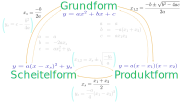
\includegraphics[width=15cm]{allg/funktionen/img/formen/formen.png}
\end{center}

\begin{bemerkung}{}{}
  Das $a$,  ist in allen Formen derselbe Wert und bestimmt die Parabelöffnung.
  \end{bemerkung}
\newpage

\textbf{Grundform aus Scheitelform} (einfaches Ausmultiplizieren). Beispiel:
$$y=2(x-3)^2-4 = 2(x^2-6x+9)-4=2x^2-12x+14$$

\begin{tabular}{rcl}
$a(x-x_S)^2+y_S$ &=& $ax^2-2ax_Sx + (ax_S^2+y_S)$\\
  $a$ &=& $a$ \\
  $b$ &=& $-2ax_S$\\
  $c$ &=& $ax_S^2+y_S$
\end{tabular}


\textbf{Grundform aus Produktform} (einfaches Ausmultiplizieren). Beispiel
$$y=2(x+3)(x-4)=2(x^2 +(3-4)x - 12) = 2x^2-x-24$$

\begin{tabular}{rcl}
  $a(x-x_1)(x-x_2)$ &=& $ax^2 - a(x_1+x_2)x + ax_1x_2$\\
  $a$ &=& $a$ \\
  $b$ &=& $-a(x_1+x_2)$\\
  $c$ &=& $ax_1x_2$
\end{tabular}


\textbf{Nullstellenform (Produktform) aus Grundform}:
Gegeben: $y = ax^2 + bx + c$

Nullstellenform: $y = a(x-x_1)\cdot{}(x-x_2)$ mit

$$x_{1,2} = \frac{-b \pm \sqrt{b^2-4ac}}{2a}$$

\begin{beispiel}{}{}
Gegeben $y = 5x^2 - 5x - 30$. Schreiben Sie dies in der Produktform (=
Nullstellenform):
\platzFuerBerechnungen{3.2}\TRAINER{$y = 5(x-3)(x+2)$\vspace{4.2cm}}
\end{beispiel}
\newpage


\textbf{Scheitelform aus Grundform}:
$$x_S=\frac{-b}{2a}$$

$y_S$ einfach durch Einsetzen von $x_S$ in die Grundform:
$$y_S=c-\frac{b^2}{4a}$$
 
\textbf{Scheitelform aus Produktform}: $x_S$ ist der Mittelwert der beiden
Nullstellen:
$$x_S=\frac{x_1+x_2}{2}$$
Danach $y_S$ einfach durch Einsetzen von $x_S$ in die Produktform:
$$y_S=\frac{-a}{4}(x_1-x_2)^2$$

\textbf{Produktform aus Scheitelform}: Einfachster Weg geht über die Grundform oder abgekürzt:
$$x_{1,2} =x_S \pm \sqrt{\frac{-y_S}{a}}$$


\subsection{Aufgaben}

\TALS{\olatLinkArbeitsblatt{Umrechnen der Formen}{https://olat.bbw.ch/auth/RepositoryEntry/572162090/CourseNode/103176133021102}{1., 2., 3. und 8.}}



\newpage

% Bereits in typ I II und III eingebaut
%\subsection{Parabel aus drei Punkten}
Vorzeigeaufgabe Marthaler Algebra S. 272 Aufg. 3. b) 


\subsection*{Aufgaben}

\AadBMTA{272}{3. a) c)}%% war Marthaler S. 187 Aufg. 676 a) und b)
\GESOAadBMTA{???}{???}

\newpage



%\newpage

%

%%%%%%%%%%%%%%%%%%%%%%%%%%%%%%%%%%%%%%%%%%%%%%%%%%%%%%%%%%%%%%%%
\subsection{Extremwertaufgaben}



\subsubsection{Aus alter Maturprüfung}

\aufgabenFarbe{Gegeben ist die Funktion $f(x) = x\cdot{}(3-\sqrt{x})$,
  $x\in[0;\infty[$.\\
  a) Bestimmen Sie die Nullstellen und das  Extremum der Funktion
  $f$.\\
  b) Im ersten Quadranten, zwischen dem  Graphen und der
  $x$-Achse ist ein  rechtwinkliges Dreieck $ABC$ einbeschrieben.  Der
  rechte Winkel ist in der Ecke $B$.  Punkt $A$ liegt im Ursprung, $B$
  auf der  $x$-Achse und $C$ auf dem Graphen von $f$. Berechnen Sie
  die Koordinaten des  Punktes $C$ so, dass der Flächeninhalt des
  Dreiecks maximal wird.
}%% END aufgabenFarbe

    
\bbwCenterGraphic{8cm}{tals/fct3/img/Maximieren.png}
\TNTeop{
   a) solve$(f(x)=0,x)$ Somit sind die Nullstellen bei 0 und 9\\
     $\text{fmax}(f(x),x)$ liefert $x=4$ ist Maximalstelle (und auch
     Maximalwert ($f(4)=4$)\\
   b) $\text{fmax}(0.5\cdot{}x\cdot{}f(x), x)$ liefert $x = 5.76$ und
   $f(5.76) = 3.456$}%% End TNTeop
\newpage
\subsection*{Aufgaben}
\AadBMTA{311}{49.}
\AadBMTA{321}{17.}

%\newpage

\section{Berührende Graphen}\index{Graphen!berührende}\index{berührende Graphen}

\textbf{Einführungsbeispiel}


Gegeben ist die Parabel $f: y=\frac{1}{4}x^2 -\frac12x +\frac14$ und von einer
Geraden $g$ ist der $y$-Achsenabschnitt $b = -2$ gegeben.

Gesucht ist von der Geraden $g$ die Steigung $a$ so, dass die
Gerade die Parabel tangiert; also genau in einem Punkt berührt.

Wo (in welchem Punkt $B=(x_B|y_B)$) tangiert also die Gerade $g$ die Parabel $f$?

In der folgenden Skizze sind drei mögliche Geraden mit $y$-Achsenabschnitt
$-2$ gezeichnet. Nur eine dieser drei Geraden \textit{tangiert} die Parabel.

\bbwGraph{-4}{4}{-3}{5}{
  \draw[thick,color=blue,variable=\x,domain=-3.5:4] plot ({\x},   {0.25*\x*\x -0.5*\x + 0.25});

  \draw[color=red,variable=\x,domain=-3:5] plot ({\x},{2*\x -2});
  \draw[color=red,variable=\x,domain=-3:5] plot ({\x},{0.5*\x - 2});
  \draw[color=cyan,thick,variable=\x,domain=-3:5] plot ({\x},{1*\x  -2});

  \bbwDot{3, 1}{green}{north}{B}

  %%%\draw[thick,color=blue,variable=\x,domain=-1:5] plot ({\x}, {0.5*\x*\x - 2*\x + 3}); 
  %%\draw[color=red,variable=\x,domain=-1:5] plot ({\x},{0.5*\x + 1});
  %%\draw[color=red,variable=\x,domain=-1:5] plot ({\x},{0.5*\x - 1.5});
  %%\draw[color=cyan,thick,variable=\x,domain=-1:6] plot ({\x},{0.5*\x  -0.125});
  %%\bbwDot{2.5, 1.125}{green}{north}{P}
}
\newpage
\textbf{Lösungsidee}: Der gesuchte Parameter ist $a$, die Steigung der
Geraden.

Nun berechne die Schnittpunkte/den Schnittpunkt mit $$f(x) = g(x).$$

Das $a$ ist gefunden, sobald die Gleichung $f(x)=g(x)$ genau eine
Lösung aufweist; dann also, wenn


\TNT{2}{die Diskriminante dieser Gleichung
verschwindet.}

Den $x$-Wert dieses Berührungspunktes nennen wir $x_B$:


Ansatz:

$$f(x_B) = g(x_B)$$

\TNT{4.4}{
 
\begin{tabular}{rclr}
$\frac14x_s^2-\frac12x_s+\frac14$          & $=$ &  $ax_s-2$ & \\
$\frac14x_s^2+(-\frac12-a)x_s + \frac94$   & $=$ & $0$       & (I)\\
\end{tabular}
\vspace{10mm}
}%% END TNT

Die Diskriminante $D=B^2 - 4AC$ muss gleich 0 sein. 

\TNT{7.2}{
$A = \frac14$, $B = -\frac12-a$ und $C = \frac94$.

  $$D=0=B^2-4AC = (-\frac12-a)^2  - (4\cdot{}A\cdot{}C)$$
  $$0 = (a^2+a+\frac14) - (4\cdot\frac14\cdot{}\frac{+9}4)$$
$$\Longrightarrow 0 = a^2 + a - 2$$
$$\Longrightarrow a_1 = 1 \text{ und  } a_2 = -2$$
\vspace{40mm}
}%% END TNT
\newpage

Für den \textbf{Berührungspunkt} $B=(x_B|y_B)$ müssen wir nun nur doch das gefundene
$a$ in die Gleichung (I) einsetzen.


\TNT{6}{
  $$0 = \frac14x_B^2 + (-\frac12 -a ) + \frac94$$

  $$x_B = x_1 = x_2 = \frac{-B \pm\sqrt{D}}{2A} = \frac{-B \pm
    \sqrt{0}}{2A} = \frac{-B}{2A}$$

  $$x_B = \frac{-B}{2A} = \frac{- (-\frac12 - a)}{\frac24} =
  \frac{\frac12 + a}{\frac12} = (\frac12 + a) : \frac12 = (\frac12+a)
  \cdot{} 2 = 1+2a$$
}



1. Fall: ($a_1=1$):

\TNT{6}{
$B_1: a_1 = 1:$
  $$x_B = 1+2a = 1 + 2\cdot{}(1) = 3$$

Das $y$ finden wir einfach durch Einsetzen von $x$ in den
Funktionsterm der Geradengleichung.

$$y_1 = a_1x_1 - 2 = 1\cdot{}3-2 = 1$$
und somit ist
$$B_1 = (3 | 1)$$
}%% END TNT



2. Fall: ($a_1=-2$):


\TNTeop{
$B_2: a_2 = -2:$
  $$x_B = 1+2a = 1 + 2\cdot{}(-2) = 1-4=-3$$


$$y_2 = a_2x_2+b = -2\cdot{}3-2 = 4$$
und somit ist
$$B_2 = (-3 | 4)$$

}%% END TNT
\newpage




\begin{rezept}{Berührende Graphen}{}

  Bei Berührungsaufgaben mit Parabeln hilft i.\,d.\,R. das folgende
  Vorgehen:

  \begin{enumerate}
  \item Funktionsterme Gleichsetzen: $$f(x) = g(x)$$
  \item In Grundform bringen: $$f(x) - g(x) = 0  \hspace{40mm}
    (I)$$
  \item Diskriminante $D = 0 $ setzen, um den Parameterwert zu
    bestimmen.
  \item Gleichung $(I)$ auflösen mit dem Wissen $D=0$.
    $$x_B=x_1=x_2= \frac{-B}{2A}$$

  \item Gefundenen Parameter in $x_B=\frac{-B}{2A}$ einsetzen, um $x$
    des Berührungspunktes zu bestimmen.
  \item Das $y_B$ des Berührungspunktes ermitteln, indem wir $x_B$ in
    $f$ oder $g$ einsetzen.
    \end{enumerate}
\end{rezept}


\TRAINER{(Je nach Zeit wäre 699. a) noch eine Vorzeigeaufgabe.)}

\subsection{Aufgaben}
\TRAINER{Achtung, dass nicht das Gleichungssystem bereits
  nach dem Gleichsetzen der Graphen aufgestellt wird. Erst nach dem
  Null-Setzen der Diskriminante erhalten wir eine gültige Gleichung
  für das Gleichungssystem.}
%%\TALSAadBMTA{190}{698., 702., 703., 705.}
\TALSAadBMTA{277}{30. a), 36. a), 40. a) c), 42. a), 43. a), 44. a)}
\newpage


\subsection{Grenzwerte und Steigungsfunktion (Optional)}

Wie macht das ein CAS, dass es den tiefsten bzw. den höchsten Punkt
einer Funktion bestimmen kann? Hier ein Erklärungsversuch am Beispiel
der quadratischen Funktion.
Betrachten wir die allgemeine quadratische Funktion $$p: y=ax^2 + bx +
c$$
Mit dem selben $a$ und dem selben $b$ kann ich eine Gerade $s$
definieren, die ich die (Tangenten-)\textbf{Steigungsfunktion}\footnote{Diese
  Steigungsfunktion wird in der Mathematik die
  \textbf{Ableitung}\index{Ableitung} genannt. Genau genommen handelt
  es sich nicht um die Steigung der Parabel, sondern um die Steigung
  einer im Punkt $P=(X_P|f(x_P))$ angelegter Tangente.} nenne:
$$s: y= 2ax+b$$
\newpage


Diese Steigungsfunktion $s$ gibt in jedem Punkt $x$ die Steigung einer
Tangente an die Parabel $p$ an.

\begin{beispiel}{Parabel}{}
  Gegeben ist die Parabel $$p: y=2.5x^2 - 3x + 6.5\text{.}$$

  Wo (für welches $x$) hat diese Parabel
  ihren Tiefpunkt? \TRAINER{Scheitelpunkt:}

  $$x_B =   \LoesungsRaumLen{8cm}{\frac{-b}{2a} = \frac{-(-3)}{2\cdot{}2.5} = 0.6}$$

  Dies ist gleichzeitig die Nullstelle der
  Steigungsfunktion:

  $$s: y= \LoesungsRaumLen{3cm}{2\cdot{}2.5x - 3}$$

  Nullstelle von $s$:

  $$x_0 = \LoesungsRaumLen{7cm}{\frac{3}{2\cdot{}2.5} = 0.6}$$

  Wir können damit aber auch die Steigung in einem ganz anderen Punkt
  \zB für $x=10$ berechnen. Die Parabel $p$ hat an der Stelle $x=10$
  die Tangentensteigung, die durch die Steigungsfunktion im Punkt $10$
  ermittelt wird:

  $$s(10) = \LoesungsRaumLen{40mm}{2\cdot{}10\cdot{2.5} - 3 = 47}$$
  
\end{beispiel}
\newpage

\begin{beispiel}{Gerade gesucht}{}
Gegeben ist die Parabel $$p: y=4x^2 -6x + 3\text{.}$$ Gesucht ist die Gerade
$g: y=ax+b$, sodass die Gerade die Parabel bei $x=7$ berührt.

\begin{enumerate}
\item Die Steigungsfunktion $s$ lautet: $$s:
  y=\LoesungsRaumLen{5cm}{2\cdot{}4x - 6}$$
  
\item Für $x=7$ hat die Steigungsfunktion den Wert \LoesungsRaumLen{1cm}{50}, und somit hat
  die Parabel bei $x=7$ die Steigung \LoesungsRaumLen{1cm}{50}.

  
\item Um den Berührungspunkt $B$ zu finden, setzen wir 7 diesen in $p$
  ein
  $$p(7)= \LoesungsRaumLen{5cm}{4\cdot{}49-6\cdot{}7+3 = 157}$$
  und somit ist
  $$B=(\LoesungsRaum{7}|\LoesungsRaum{157})$$
  
\item Die gesuchte Gerade $g: y=ax+b$ hat also auch die Steigung \LoesungsRaum{50}
  und verläuft durch den Berührungspunkt $B=(\LoesungsRaumLen{9mm}{7}|\LoesungsRaumLen{11mm}{157})$. Also
  $$\LoesungsRaumLen{7cm}{157=50\cdot{}7+b}$$

  Somit ist das gesuchte
  $$b = \LoesungsRaumLen{55mm}{157-50\cdot{}7=-193}$$
  
  und die gesuchte Funktionsgleichung der Geraden lautet: $$y = \LoesungsRaumLen{22mm}{50x-193}$$
  \end{enumerate}
\end{beispiel}

\TRAINER{Idee: Auf mm-Papier eine Funktion $y=\frac1{27}x^3-\frac19
  x^2 - \frac89 x$ vorgeben.

Auftrag: Legen Sie in 5 Punkten eine Tangente an die Funktion und
bestimmen Sie deren Steigung.
Tragen Sie die Steigung in ein neues Koordinatensystem ein: $x$-Achse
= $x$ Wert, $y$-Achse = Steigung der Funktion.
$$f' : y = \frac19 (x-1)^2 - 1 $$
}%%
\newpage

\subsubsection{Beweis der Formel der (Tangenten-)Steigungsfunktion}

Betrachten wir auf auf der $x$-Achse zwei benachbarte Punkte $x$ und
$x+\Delta$. Die Funktionswerte lauten $f(x)$ und $f(x+\Delta)$. Die
\textbf{Steigung} kann nun für eine Gerade bestimmt werden durch:

\bbwCenterGraphic{7cm}{tals/fct3/img/Steigungsfunktion.jpg}

$$\frac{f(x+\Delta) - f(x)}{\Delta}$$

Dies gilt für eine Parabel $p: y=ax^2+bx+c$ näherungsweise auch:
$$\frac{f(x+\Delta)-f(x)}{\Delta} = \frac{(a(x+\Delta)^2 + b(x+\Delta)
  + c) - (ax^2 + bx +c)}{\Delta}=2ax+a\Delta+b$$

Wenn wir nun das $\Delta$ gegen Null gehen lassen, also immer kleinere
Werte einsetzen, so verschwindet der Term $a\cdot{}\Delta$ fast und unsere
Formel stimmt annähernd --- jedoch präzise genug, um dies als Beweis
gelten zu lassen.

Ein anderer Beweis wäre die Tangente effektiv einzusetzen und diese so
zu wählen, dass es genau einen Schnittpunkt gibt, was wieder darauf
zurückführt, dass die Diskriminante = Null gesetzt werden muss. Dann
sind wir exakt, aber der Beweis ist ungleich aufwändiger.
\newpage


\newpage



%% Metapackaeg Planimetrie I
%%%%%%%%%%%%%%%55
%% Funktionen II TALS Metapackage
\part{Funktionen II}\index{Funktionen!II|textbf}
\renewcommand{\bbwPartID}{FCT2}
%%
%% 2019 07 04 Ph. G. Freimann
%%

\section{Quadratische Funktionen}\index{Funktionen!quadratische}
\sectuntertitel{Geraden im Lande der Parabeln wird dringend angeraten, einen
  Integrationskurs zu besuchen.}
%%%%%%%%%%%%%%%%%%%%%%%%%%%%%%%%%%%%%%%%%%%%%%%%%%%%%%%%%%%%%%%%%%%%%%%%%%%%%%%%%

%%\bbwCenterGraphic{8cm}{tals/fct2/img/lugano2018.jpg}
%%\textit{Bildlegende: Parabeln in Lugano (2018)}
\bbwCenterGraphic{175mm}{tals/fct2/img/paris2022.jpg}
\textit{Bildlegende: Parabeln in den Gärten von Versailles (2022)}

\subsection*{Lernziele}

\begin{itemize}
\item Definition
\item Formen: Scheitel-, Produkt-, Normalform
\item Graphische Darstellung
\item Translationen und Spiegelungen
\end{itemize}

\TadBMTA{260}{15}
%%\TALS{(\cite{frommenwiler17alg} S.183 (Kap. 3.4))}
%%\GESO{(\cite{marthaler21alg}       S.260 (Kap. 15))}

Einstieg: Bilder von Heimgartner/Hunziker.


\textbf{Einstiegsaufgabe: } \aufgabenFarbe{Lösen Sie Aufgaben 1. und 2.
  von Seite 272: Welche der angegebenen Funktionen sind quadratisch?}

\newpage

\subsection{Parabel}\index{Parabel}\index{Normalparabel}

Zeichnen Sie die Funktionen $f: y=x^2$ (= Normalparabel), $y=\frac{1}{3}x^2$

und $y=-0.25\cdot{}x^2$  ins Koordinatensystem:

\bbwGraph{-3}{3}{-3}{7}{
  \TRAINER{\bbwFuncC{\x * \x}{-2.5:2.5}{green}
    \bbwFuncC{-0.25*\x * \x}{-3:3}{green}
    \bbwFuncC{\x * \x / 3}{-3:3}{green}
  }
}


\newpage

\subsection{Grundform}\index{Grundform!quadratische Funktion}\index{Quadratische Funktion!Grundform}
Die Funktion $f(x): x \mapsto y = ax^2 + bx +c$ ist eine
quadratische Funktion in Grundform\index{Grundform!quadratische Funktion}.

Spielen Sie mit \TALS{dem TI-nSpire oder mit} \texttt{geogebra.org} an den Parametern $a$, $b$ und $c$ der Funktionsgleichung $y = a\cdot{}x^2 + b\cdot{} x + c$ herum. Was bewirkt der Parameter

$a$: \LoesungsRaumLang{Parabelöffnung: $|a|$ klein: Breite (weite) Öffnung / $|a|$ groß: Enge, schmale Öffnung. $a < 0$: Parabel ist nach unten geöffnet. $a > 0$: Parabel ist nach oben geöffnet.}

$b$: \LoesungsRaumLang{«Parabelsteigung»\footnote{Mit «Parabelsteigung» ist hier die Steigung der entsprechenden Tangente gemeint.} im Punkt $A(0|c)$}

$c$: \LoesungsRaumLang{$y$-Achsenabschnitt. Damit wird eine Verschiebung der Parabel entlang der $y$-Achse erreicht.}

Versuchen Sie eine Parabel mit Scheitelpunkt $(1|1)$ zu finden\TRAINER{(Lösung: $b=-2a$ und $a+b+c=1$.)}.

\subsection*{Aufgaben}
%%\TALSAadBMTA{184ff}{660. a) c) f), 662. a) b) c) und e)}
\AadBMTA{273}{5., 6., 7., 8. und 9.}
\newpage

\subsection{Vier charakteristische Punkte}
Zeichnen Sie die Funktion
$$p: y = x^2 - 4x + \frac{7}{4}$$

\bbwGraph{-3}{6}{-3}{2}{
\TRAINER{\bbwFunc{\x*\x - 4*\x + 1.75}{-0.2:4}}
}%% end BBW Graph

Wo befinden sich die charakteristischen Punkte?

\TNT{2.4}{\vspace{24mm}}


Die charakteristischen Punkte sind:
\begin{itemize}
\item Schnittpunkt mit $y$-Achse = (\LoesungsRaum{0} | \LoesungsRaum{1.75})
\item Nullstellen: $N_1=(\LoesungsRaum{0.5}| \LoesungsRaum{0}), N_2=( \LoesungsRaum{3.5}|\LoesungsRaum{0})$
\item Scheitelpunkt: $S=(\LoesungsRaum{2}|\LoesungsRaum{-2.25})$
\end{itemize}
 
Wie berechnen sich nun diese Punkte?
\newpage
\subsubsection{Parabelöffnung}
Eigentlich ist die Parabelöffnung kein charakteristischer
Punkt. Dennoch kann man eine $x$-Einheit vom Scheitelpunkt entfernt,
das $a$ der Grundform ($y=ax^2+bx+c$) direkt ablesen. Gehen wir bei
der Normalparabel ($a=1$) vom
Scheitelpunkt um eine Einheit nach rechts, so muss die Parabel um eine
$y$-Einheit nach oben anwachsen.

\TNT{10}{
Parabel durch Scheitelpunkt $P=(-3|1)$ und durch $(-2|2)$ =
verschobene Normalparbel zeichnen.

Parabel mit Scheitelpunkt $P=(2|2)$ durch $(3|0.5)$ zeichnen. Das $a$
ist somit sofort $a=-1.5$ abzulesen.
}

\subsubsection{$y$-Achsenabschnitt}
Genau wie bei der linearen Funktion, gilt für den $y$-Achsenabschnitt,
dass die $x$-Koordinate dieses Punktes Null ist.
$$y = x^2 -4x + 1.75$$
wird mit $x=0$ zu
$y = 1.75$.

Der $y$-Achsenabschnitt ist somit immer das $c$ aus $y = ax^2 + bx +
c$.

\newpage

\subsubsection{Nullstellen}
Wie bei den linearen Funktionen sind auch hier die
Nullstellen die Schnittpunkte mit der $x$-Achse. Dies bedeutet für die
Nullstellen $N(x_0 | y_0)$, dass die $y$-Koordinate = 0 ist. Es gilt
also

$$0 = x^2 - 4 x + \frac{7}{4} $$

Dies ist eine quadratische Gleichung mit den Lösungen:

$$x_{1,2} = \frac{-b \pm \sqrt{b^2-4ac}}{2a}$$ 

\noTRAINER{\platzFuerBerechnungen{2.4}}
\TRAINER{$x_{1} = 0.5; x_{2}=3.5$ (Mitternachtsformel)
  \vspace{3cm}}

\begin{bemerkung}{}{}
  Die Nullstellen der quadratischen Funktion entsprechen den Lösungen
  der zugehörigen quadratischen Funktion (mit $y=0$). Daher gilt
  auch hier: 


  \begin{tabular}{c|p{8cm}}
    Diskriminante $D=b^2-4ac$ > 0 & Es gibt zwei Nullstellen. \\
    \hline\\
    Diskriminante $D=b^2-4ac$ = 0 & Es gibt eine Nullstelle, denn der Scheitelpunkt liegt auf der $x$-Achse.\\
    \hline\\
    Diskriminante $D=b^2-4ac$ < 0 & Es gibt keine Nullstellen, denn die Parabel schneidet die $x$-Achse nicht.\\
  \end{tabular}
  
 \ifisALLINONE{Zum Begriff \textbf{Diskriminante}:  \totalref{diskriminante}}\fi{} 
\end{bemerkung}

\subsection*{Aufgaben}
\AadBMTA{277ff}{28. a) c) }

\newpage



\subsubsection{Scheitelpunkt}\index{Scheitelpunkt}
Der Tief- bzw. Hochpunkt einer Parabel wird \textbf{Scheitelpunkt}
genannt.

Wir berechnen den Scheitelpunkt in zwei Schritten.

\textbf{Erstens:} Wir berechnen den Mittelwert der beiden Nullstellen:
$$x_S := \frac{x_{1} + x_{2}}{2} = \frac{\frac{-b+\sqrt{D}}{2a} + \frac{-b-\sqrt{D}}{2a}}{2} =
\frac{(-b+\sqrt{D}) + (-b-\sqrt{D})}{4a} =\frac{-b}{2a}$$
Dabei ist $D$ die Diskriminante $D=b^2-4ac$.

\platzFuerBerechnungen{2.4}
\TRAINER{$x_S = 2$
\vspace{3cm}}

\textbf{Zweitens:} Wir setzen den gefundenen $x$-Wert
(\LoesungsRaum{2}) in die Funktionsgleichung
ein:
$$y_S = x^2 - 4x + 1.75$$
$$y_S = (\LoesungsRaum{2})^2 - 4\cdot{}(\LoesungsRaum{2}) + 1.75$$

Wir erhalten für den Scheitelpunkt $S$: $S=(x_S | y_S) = (\LoesungsRaum{2} | \LoesungsRaum{-2.25})$.

\begin{gesetz}{Scheitelpunkt}{}
  Der Scheitelpunkt $S$ einer Parabel in der Grundform ($y=ax^2+bx+c$) kann wie folgt
  berechnet werden:

  $$S=\left(\frac{-b}{2a}\middle|\frac{4ac-b^2}{4a}\right)$$

  (Bem.: Der $y$-Wert kann einfach durch Einsetzen des $x$-Wertes in
  die Funktionsgleichnug gefunden werden.)
  \end{gesetz}
  
\subsection*{Aufgaben}
%%\TALSAadBMTA{184ff}{665. a) b) c) 666. a) b) c) e) f) g)}
\AadBMTA{273}{4. (=Aufg. 22. S. 276)}

\newpage

\subsection{Bestimmen der Funktionsgleichung}
\TALS{S. 187 Kap. 3.4.3}

\subsubsection{Referenzaufgaben}

\textbf{TYP I}

Gegeben ist ein Punkt $P$ mit den Koordinaten $(2.3 | -1.5)$. Gesucht ist die reinquadratische Funktion $f: y=a\cdot{}x^2$, welche durch diesen Punkt geht.
Machen Sie vorab eine Skizze.

\bbwGraph{-3}{3}{-2}{1}{
  \TRAINER{\bbwFunc{-0.2836 * \x * \x}{-2.5:2.5}
    \bbwDot{2.3,-1.5}{blue}{west}{P}
  }%% end TRAINER
}%% end BBW Graph

\platzFuerBerechnungen{3.6}

\TRAINER{Idee: Punkt einsetzen: $-1.5 = a\cdot{}(2.3)^2$. Das Auf"|lösen dieser Gleichung liefert $a = \frac{-1.5}{2.3^2}$. Dies liefert $a\approx -0.2836$}

Weitere «TYP 1» Aufgaben wären z. B. $y = 3x^2 - bx + 4$ oder $y=2x^2
-7x + c$ mit anderen Worten alle Parabeln mit genau \textbf{einem}
Parameter, daher «Typ 1».

\newpage



\textbf{TYP II}

Gegeben sind zwei Punkte und wir haben zwei Unbekannte.

\begin{rezept}{}{}
  Gesucht sind $a$ und $c$ aus $y = ax^2 + c$ bei den gegebenen
  Punkten $(7|5)$ und $(2|-4)$.

  Wir lösen dies auch durch Einsetzen der Punkte in die
  Funktionsgleichung und wir erhalten zwei Gleichungen:


  \begin{tabular}{c | r  c  r |}
    (I)  &  $5$ & = & $(7)^2\cdot{} a + c$ \\
    (II) & $-4$ & = &  $(2)^2\cdot{} a + c$ \\
  \end{tabular}

  Durch Subtrahieren der Gleichungen erhalten wir

  \begin{tabular}{c | r  c  r | c}
    (I)  &  $5$ & = & $49\cdot{} a + c$ & \,\\
    (II) & $-4$ & = &  $4\cdot{} a + c$ & $\ominus$\\
  \end{tabular}

  $$9 = 45a$$ und somit
  $$a =\frac{1}{5}.$$

  Dieses $a$ (= $\frac{1}{5}$) setzen wir nun in eine der Gleichungen
  (\zB (I)) ein und erhalten
  $$5=49\cdot{}\frac{1}{5} + c$$
  und nach Auf"|lösen erhalten wir $c=\frac{-24}{5}$.

  Die gesuchte Gleichung lautet also:

  $$y = \frac{1}{5}x^2 - \frac{24}{5}$$
\end{rezept}

Probe durch Einsetzen der $x$-Werte der Punkte in die gefundene Funktionsgleichung:

\TNTeop{}
%%\newpage

\begin{beispiel}{}{}
  Anstelle von $a$ und $c$ können natürlich auch $a$ und $b$ gesucht
  sein. Daher eine zweite Aufgabe.

  Gesucht sind $a$ und $b$ aus $y = ax^2 + bx$ bei den gegebenen

  Punkten $(2|-6)$ und $(-3|5)$.

  Wir lösen dies wiederum durch Einsetzen der Punkte in die
  Funktionsgleichung und wir erhalten die beiden Gleichungen, welche
  wir durch das Additionsverfahren lösen können:

  \begin{tabular}{c | r  c  r | c}
    (I)  &  $-6$ & = & $4a + 2b$ & $\cdot{} 3$ \\
    (II) &   $5$ & = & $9a - 3b$ & $\cdot{} 2$ \\
  \end{tabular}

  somit:
  
  \begin{tabular}{c | r  c  r | c}
    (I')  & $-18$ & = & $12a + 6b$ &\, \\
     \,   & \,    & \,&   \,       & $\oplus$\\
    (II') &  $10$ & = & $18a - 6b$ &\, \\
  \end{tabular}

  Nach Addition der Gleichungen erhalten wir

  $$-8 = 30a$$

  was uns zu $a=\frac{-4}{15}$ bringt.

Dieses $a$ können wir nun wieder in eine der beiden Gleichungen
einsetzen (\zB in (I)):

$$-6=4\cdot{}\frac{-4}{15} + 2b$$

Das Auf"|lösen obiger Gleichung liefert nach Kürzen: $b=\frac{-37}{15}$.

Die gesuchte Funktionsgleichung lautet also

$$y = \frac{-4}{15} x^2 - \frac{37}{15} x.$$

\end{beispiel}

Auch bei «Typ II» kann natürlich jede \textbf{zwei}parametrige quadratische
Funktion herhalten, wie \zB $y=-6cx^2 + bx - c$ durch \textbf{zwei}
gegebene Punkte.
\newpage


\textbf{TYP III}: Gegeben sind hier drei Punkte, wir haben aber auch
drei Unbekannte in $y = ax^2 + bx + c$. Die Punkte sind hier
(1|3), (2|3.5) und (-3|11).

Durch Einsetzen der drei Punkte je in die Funktionsgleichung erhalten
wir drei Gleichungen:

\begin{tabular}{c|r c rcrcr|}
  (I)   & 3   & = & $(1)^2\cdot{}a$  &$+$& $(1)\cdot{}b$  &$+$& c \\ 
  (II)  & 3.5 & = & $(2)^2\cdot{}a$  &$+$& $(2)\cdot{}b$  &$+$& c \\ 
  (III) & 11  & = & $(-3)^2\cdot{}a$ &$+$& $(-3)\cdot{}b$ &$+$& c \\ 
\end{tabular}

Vereinfachen:

\begin{tabular}{c|r c rcrcr|}
  (I)   & 3   & = & $a$  &$+$& $b$  &$+$& c \\ 
  (II)  & 3.5 & = & $4a$ &$+$& $2b$ &$+$& c \\ 
  (III) & 11  & = & $9a$ &$-$& $3b$ &$+$& c \\ 
\end{tabular}

Nun finden wir $a$, indem wir zunächst $c$ durch Subtraktion
eliminieren:

\begin{tabular}{l|r c rcr|}
  (IV) = (II) -   (I) & 0.5  & = & $3a$ &$+$& $b$ \\ 
  (V)  = (III) - (II) & 7.5  & = & $5a$ &$-$& $5b$ \\ 
\end{tabular}

Multiplizieren wir nun die Gleichung (IV) mit 5, so erhalten wir

\begin{tabular}{r|r c rcr|}
  5$\cdot{}$(IV)  & 2.5  & = & $15a$ &$+$& $5b$ \\ 
  (V)             & 7.5  & = & $5a$  &$-$& $5b$ \\ 
\end{tabular}

Durch Addition der beiden Gleichungen (IV) und (V) erhalten wir

$10 = 20a$ oder $a = \frac{1}{2}$.

Um $b$ zu finden, setzen wir $a = \frac{1}{2}$ in (V) ein: $7.5 =
5\cdot{}\frac{1}{2} - 5b$.

Auf"|lösen nach $b$ ergibt $b = -1$.

Zu guter Letzt setzen wir $a = \frac{1}{2}$ und $b=-1$ in die
Gleichung (I) ein, um noch $c$ zu erhalten:

$$3 = a + b + c = \frac{1}{2} - 1 + c$$

Somit ist $c=3.5$ und die Funktionsgleichung lautet:

$$y = \frac{1}{2}x^2 - x + 3.5$$


\TALS{\subsection*{Aufgaben}}
%%\TALSAadBMTA{187ff}{676. a) c), 682., 684.}
\AadBMTA{272}{3. a) c), 20. a) c), 21., 22., 24. a), 25. b)}
\newpage


\subsection{Computer Algebra Systeme (CAS)}\index{CAS}
Das eben gezeigte Beispiel wird in der Praxis meist nicht von Hand,
sondern mit einem Computer-Algebra-System, kurz CAS, gelöst:

\paragraph{Aufgabenstellung}
Gegeben sind wieder drei Punkte (1|3), (2|3.5) und (-3|11).
Gesucht ist die Parabel $y = ax^2 + bx + c$, welche durch die drei
Punkte geht.

Dies wird mit dem \tinspire{} wie folgt gelöst:
\begin{itemize}
\item Definiere die Funktionsgleichung mit
  Parametern\footnote{\tinspire Regel: $ax\ne a\cdot{} x$}:\\
  $$f(x) := a\cdot{}x^2 + b\cdot{}x + c$$
\item Definiere das Gleichungssystem:
  $$gls := \left\{ \begin{array}{l}
    f(1) = 3\\
    f(2) = 3.5\\
    f(-3)= 11\\
  \end{array}\right.$$
\item Löse das Gleichungssystem:
  $$solve(gls,\{a, b, c\})$$
\end{itemize}

\subsection*{Aufgaben}
\AadBMTA{272}{3. b) d)}

\newpage

\subsection{Formen der quadratischen Funktion}
\subsubsection{Nullstellenform}\index{Nullstellenform}

Die \textbf{Nullstellenform} wird auch  «faktorisierte Form» oder
«Produktform» genannt.\index{faktorisierte Form}\index{Produktform}

Beachten Sie die folgende quadr. Funktionsgleichung:

$$y = 3.1(x-5)(x+6)$$

Dies ist eine quadratische Funktion in der sogenannten
\textbf{Nullstellenform}, denn die Nullstellen (hier $x_0 = 5$ oder
$x_0 = -6$) können direkt aus der Funktionsgleichung abgelesen werden.
Wenn wir $y=0$ in die Gleichung setzen (Nullstelle),

$$0 = 3.1(x-5)(x+6)$$
so wird die Gleichung genau dann wahr, wenn (mind.) einer der beiden Klammerausdrücke rechts
gleich Null ist. Die Parabelöffnung (hier 3.1) kann dabei beliebig variieren und ist (neben den Nullstellen) der einzige Parameter.

Die Nullstellenform lautet

\begin{gesetz}{}{}

  $$y = a(x-x_1)\cdot{}(x-x_2)$$

  \end{gesetz}

wobei $x_1$ und $x_2$ die Nullstellen der Parabel bezeichnen. 
\newpage


\subsubsection*{Referenzaufgabe zur Nullstellenform}

\noTRAINER{\bbwGraphic{16cm}{tals/fct2/img/BrunnenNullstellenformOhneKoordinatensystem.png}}
\TRAINER{\bbwGraphic{16cm}{tals/fct2/img/BrunnenNullstellenformMitKoordinatensystem.png}}

Ein parabelförmiger Wasserstrahl spritzt ebenerdig aus einem Brunnen und trifft 7m von der Düse entfernt wieder auf dem Boden auf.
Das Wasser steigt also erst gleich hoch an, wie es danach wieder «herunterfällt».
Dabei wird gemessen, dass 1m von der Düse entfernt der Wasserstrahl 84cm über Boden verläuft.
Können Sie aufrecht unter dem Wasserstrahl hindurchgehen?

Tipp: Skizze und  die Parabelgleichung in Nullstellenform aufschreiben. Die Düse ist der Ursprung der Koordinatensystems.\\

\TNT{5.2}{Die Funktionsgleichung lautet $y=a(x-x_1)(x-x2)$.\\
  Mit den Nullstellen $x_1=0$ und $x_2=7$.\\
  Wir setzen den gemessenen Punkt (1|0.84) in die Gleichung ein und erhalten $0.84 = a\cdot{}(1-0)(1-7)$.\\
  Daraus ergibt sich $a=0.84/(-6) = -0.14 $.\\
  Nun setzen wir 3.5 Meter in die Funktionsgleichung $y = -0.14(x-0)(x-7)$ ein: und erhalten $y=-01.4\cdot{}3.5\cdot{}(-3.5) = 1.715m$; das ist die höchste Parabelstelle.}


\subsection*{Aufgaben}%% Nullstellenform
%%\TALSAadBMTA{185}{663, 678., 680.}
\TALSAadBMTA{277}{30. a) b), 31. b)}
\newpage

%%\TRAINER{\, \newpage}
\subsubsection{Scheitelform}\index{Scheitelform!der quadratischen
  Funktion}
Einstieg: Wo hat die Parabel $f: y=3.6(x-4)^2 + 5$ ihren
Scheitelpunkt?

\TNT{4.4}{CAS: bei $x_S = 4$ und $y_S= 5$; völlig irrelevant ist die 3.6.}

Ist eine quadratische Funktion in der Form
\begin{gesetz}{}{}
$$y = a(x-x_S)^2 + y_S$$
\end{gesetz}
gegeben, so sprechen wir von der \textbf{Scheitelform} oder Scheitelpunktsform.
Das liegt daran, dass diese Parabel ihren Scheitelpunkt bei
$(x_S|y_S)$ hat.

Setzen wir für $x$ = $x_S$ in die Funktionsgleichung, so erhalten wir
gerade die $y$-Koordinate des Scheitelpunktes. Je weiter wir uns nun
mit $x$ von $x_S$ wegbewegen, umso größer wird der Term $(x-x_S)^2$
und zwar in egal welcher Richtung wir uns von $x_S$ wegbewegen, die
$y$-Koordinate verhält sich in beiden Fällen symmetrisch.

Prüfen Sie dies mit TI-nSpire oder \texttt{geogebra.org} an der Funktion

$$y = a\cdot{}(x-p)^2 + q$$

Definieren Sie dabei auch den Punkt $S=(p|q)$. Spielen Sie nun mit
$a$, $p$ und $q$. Was bewirken die Änderungen?
\newpage


\subsubsection{Referenzaufgabe Scheitelform}
Von einer Parabel ist der Scheitel $S(2|3)$ gegeben. Ebenfalls ist bekannt, dass die Parabel durch den Punkt $P\left(-\frac{1}{2}\middle|1\right)$ geht.

  Berechnen Sie die Funktionsgleichung in der Grundform $y = ax^2 + bx + c$. Tipp:
  Schreiben Sie die Funktionsgleichung in der Form $y=a(x - x_S)^2 +  y_S$ und setzen anschließend den Punkt $P$ ein.

  \platzFuerBerechnungen{8.0}%%
  \TRAINER{
    Ansatz:
    $$y = a(x-2)^2 + 3$$
    Jetzt $P$ einsetzen:
    $$1 = a(-\frac{1}{2} - 2)^2 + 3 $$
    Nach $a$ auf"|lösen ergibt:
    $$a=-0.32 (=\frac{-2}{2.5^2})$$
    Nun setzen wir $a=-0.32$ in die Funktionsgleichung $y=a(x-2)^2+3$
    ein:
    $$y=-0.32(x-2)^2+3$$
    und quadrieren das Binom, um die geforderte Grundform zu erhalten:
    $$y = -0.32(x^2 - 4x + 4) + 3 = -0.32x^2 + 1.28x + 1.72$$
  }%%end TRAINER%%

  \subsection*{Aufgabe}
  \AadBMTA{277}{29. a) c) e), 32. a), 33.}
%%  \TALSAadBMTA{185}{679. a), 681., 695., 684. a), 700., 694., 686.(*) und  664.}}

\newpage


\subsection{Umrechnungen der Formen}\index{Formen!der quadratischen Funktion}\index{Quadratische Funktion!Formen}

Nochmals die drei Formen im Überblick:


\begin{tabular}{c|l}
  Form & Funktionsgleichung\\
  \hline\\
  Normalform/Grundform & $f: y= ax^2 + bx + c$\\
  \hline\\
  Nullstellenform, faktorisierte Form oder Produktform & $f: y=a(x-x_0)(x-x_1)$\\
  \hline\\
  Scheitelform & $f: y=a(x-x_S)^2+y_S$\\
  \hline%%
\end{tabular}


\subsubsection{Umrechnungen zwischen den Formen}\index{Umrechnungen!quadratische Funktion}\index{Quadratische Funktion!Umrechnungen}

\begin{center}
  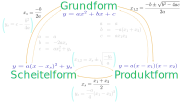
\includegraphics[width=15cm]{allg/funktionen/img/formen/formen.png}
\end{center}

\begin{bemerkung}{}{}
  Das $a$,  ist in allen Formen derselbe Wert und bestimmt die Parabelöffnung.
  \end{bemerkung}
\newpage

\textbf{Grundform aus Scheitelform} (einfaches Ausmultiplizieren). Beispiel:
$$y=2(x-3)^2-4 = 2(x^2-6x+9)-4=2x^2-12x+14$$

\begin{tabular}{rcl}
$a(x-x_S)^2+y_S$ &=& $ax^2-2ax_Sx + (ax_S^2+y_S)$\\
  $a$ &=& $a$ \\
  $b$ &=& $-2ax_S$\\
  $c$ &=& $ax_S^2+y_S$
\end{tabular}


\textbf{Grundform aus Produktform} (einfaches Ausmultiplizieren). Beispiel
$$y=2(x+3)(x-4)=2(x^2 +(3-4)x - 12) = 2x^2-x-24$$

\begin{tabular}{rcl}
  $a(x-x_1)(x-x_2)$ &=& $ax^2 - a(x_1+x_2)x + ax_1x_2$\\
  $a$ &=& $a$ \\
  $b$ &=& $-a(x_1+x_2)$\\
  $c$ &=& $ax_1x_2$
\end{tabular}


\textbf{Nullstellenform (Produktform) aus Grundform}:
Gegeben: $y = ax^2 + bx + c$

Nullstellenform: $y = a(x-x_1)\cdot{}(x-x_2)$ mit

$$x_{1,2} = \frac{-b \pm \sqrt{b^2-4ac}}{2a}$$

\begin{beispiel}{}{}
Gegeben $y = 5x^2 - 5x - 30$. Schreiben Sie dies in der Produktform (=
Nullstellenform):
\platzFuerBerechnungen{3.2}\TRAINER{$y = 5(x-3)(x+2)$\vspace{4.2cm}}
\end{beispiel}
\newpage


\textbf{Scheitelform aus Grundform}:
$$x_S=\frac{-b}{2a}$$

$y_S$ einfach durch Einsetzen von $x_S$ in die Grundform:
$$y_S=c-\frac{b^2}{4a}$$
 
\textbf{Scheitelform aus Produktform}: $x_S$ ist der Mittelwert der beiden
Nullstellen:
$$x_S=\frac{x_1+x_2}{2}$$
Danach $y_S$ einfach durch Einsetzen von $x_S$ in die Produktform:
$$y_S=\frac{-a}{4}(x_1-x_2)^2$$

\textbf{Produktform aus Scheitelform}: Einfachster Weg geht über die Grundform oder abgekürzt:
$$x_{1,2} =x_S \pm \sqrt{\frac{-y_S}{a}}$$


\subsection{Aufgaben}

\TALS{\olatLinkArbeitsblatt{Umrechnen der Formen}{https://olat.bbw.ch/auth/RepositoryEntry/572162090/CourseNode/103176133021102}{1., 2., 3. und 8.}}



\newpage

% Bereits in typ I II und III eingebaut
%\subsection{Parabel aus drei Punkten}
Vorzeigeaufgabe Marthaler Algebra S. 272 Aufg. 3. b) 


\subsection*{Aufgaben}

\AadBMTA{272}{3. a) c)}%% war Marthaler S. 187 Aufg. 676 a) und b)
\GESOAadBMTA{???}{???}

\newpage



%\newpage

%

%%%%%%%%%%%%%%%%%%%%%%%%%%%%%%%%%%%%%%%%%%%%%%%%%%%%%%%%%%%%%%%%
\subsection{Extremwertaufgaben}



\subsubsection{Aus alter Maturprüfung}

\aufgabenFarbe{Gegeben ist die Funktion $f(x) = x\cdot{}(3-\sqrt{x})$,
  $x\in[0;\infty[$.\\
  a) Bestimmen Sie die Nullstellen und das  Extremum der Funktion
  $f$.\\
  b) Im ersten Quadranten, zwischen dem  Graphen und der
  $x$-Achse ist ein  rechtwinkliges Dreieck $ABC$ einbeschrieben.  Der
  rechte Winkel ist in der Ecke $B$.  Punkt $A$ liegt im Ursprung, $B$
  auf der  $x$-Achse und $C$ auf dem Graphen von $f$. Berechnen Sie
  die Koordinaten des  Punktes $C$ so, dass der Flächeninhalt des
  Dreiecks maximal wird.
}%% END aufgabenFarbe

    
\bbwCenterGraphic{8cm}{tals/fct3/img/Maximieren.png}
\TNTeop{
   a) solve$(f(x)=0,x)$ Somit sind die Nullstellen bei 0 und 9\\
     $\text{fmax}(f(x),x)$ liefert $x=4$ ist Maximalstelle (und auch
     Maximalwert ($f(4)=4$)\\
   b) $\text{fmax}(0.5\cdot{}x\cdot{}f(x), x)$ liefert $x = 5.76$ und
   $f(5.76) = 3.456$}%% End TNTeop
\newpage
\subsection*{Aufgaben}
\AadBMTA{311}{49.}
\AadBMTA{321}{17.}

%\newpage

\section{Berührende Graphen}\index{Graphen!berührende}\index{berührende Graphen}

\textbf{Einführungsbeispiel}


Gegeben ist die Parabel $f: y=\frac{1}{4}x^2 -\frac12x +\frac14$ und von einer
Geraden $g$ ist der $y$-Achsenabschnitt $b = -2$ gegeben.

Gesucht ist von der Geraden $g$ die Steigung $a$ so, dass die
Gerade die Parabel tangiert; also genau in einem Punkt berührt.

Wo (in welchem Punkt $B=(x_B|y_B)$) tangiert also die Gerade $g$ die Parabel $f$?

In der folgenden Skizze sind drei mögliche Geraden mit $y$-Achsenabschnitt
$-2$ gezeichnet. Nur eine dieser drei Geraden \textit{tangiert} die Parabel.

\bbwGraph{-4}{4}{-3}{5}{
  \draw[thick,color=blue,variable=\x,domain=-3.5:4] plot ({\x},   {0.25*\x*\x -0.5*\x + 0.25});

  \draw[color=red,variable=\x,domain=-3:5] plot ({\x},{2*\x -2});
  \draw[color=red,variable=\x,domain=-3:5] plot ({\x},{0.5*\x - 2});
  \draw[color=cyan,thick,variable=\x,domain=-3:5] plot ({\x},{1*\x  -2});

  \bbwDot{3, 1}{green}{north}{B}

  %%%\draw[thick,color=blue,variable=\x,domain=-1:5] plot ({\x}, {0.5*\x*\x - 2*\x + 3}); 
  %%\draw[color=red,variable=\x,domain=-1:5] plot ({\x},{0.5*\x + 1});
  %%\draw[color=red,variable=\x,domain=-1:5] plot ({\x},{0.5*\x - 1.5});
  %%\draw[color=cyan,thick,variable=\x,domain=-1:6] plot ({\x},{0.5*\x  -0.125});
  %%\bbwDot{2.5, 1.125}{green}{north}{P}
}
\newpage
\textbf{Lösungsidee}: Der gesuchte Parameter ist $a$, die Steigung der
Geraden.

Nun berechne die Schnittpunkte/den Schnittpunkt mit $$f(x) = g(x).$$

Das $a$ ist gefunden, sobald die Gleichung $f(x)=g(x)$ genau eine
Lösung aufweist; dann also, wenn


\TNT{2}{die Diskriminante dieser Gleichung
verschwindet.}

Den $x$-Wert dieses Berührungspunktes nennen wir $x_B$:


Ansatz:

$$f(x_B) = g(x_B)$$

\TNT{4.4}{
 
\begin{tabular}{rclr}
$\frac14x_s^2-\frac12x_s+\frac14$          & $=$ &  $ax_s-2$ & \\
$\frac14x_s^2+(-\frac12-a)x_s + \frac94$   & $=$ & $0$       & (I)\\
\end{tabular}
\vspace{10mm}
}%% END TNT

Die Diskriminante $D=B^2 - 4AC$ muss gleich 0 sein. 

\TNT{7.2}{
$A = \frac14$, $B = -\frac12-a$ und $C = \frac94$.

  $$D=0=B^2-4AC = (-\frac12-a)^2  - (4\cdot{}A\cdot{}C)$$
  $$0 = (a^2+a+\frac14) - (4\cdot\frac14\cdot{}\frac{+9}4)$$
$$\Longrightarrow 0 = a^2 + a - 2$$
$$\Longrightarrow a_1 = 1 \text{ und  } a_2 = -2$$
\vspace{40mm}
}%% END TNT
\newpage

Für den \textbf{Berührungspunkt} $B=(x_B|y_B)$ müssen wir nun nur doch das gefundene
$a$ in die Gleichung (I) einsetzen.


\TNT{6}{
  $$0 = \frac14x_B^2 + (-\frac12 -a ) + \frac94$$

  $$x_B = x_1 = x_2 = \frac{-B \pm\sqrt{D}}{2A} = \frac{-B \pm
    \sqrt{0}}{2A} = \frac{-B}{2A}$$

  $$x_B = \frac{-B}{2A} = \frac{- (-\frac12 - a)}{\frac24} =
  \frac{\frac12 + a}{\frac12} = (\frac12 + a) : \frac12 = (\frac12+a)
  \cdot{} 2 = 1+2a$$
}



1. Fall: ($a_1=1$):

\TNT{6}{
$B_1: a_1 = 1:$
  $$x_B = 1+2a = 1 + 2\cdot{}(1) = 3$$

Das $y$ finden wir einfach durch Einsetzen von $x$ in den
Funktionsterm der Geradengleichung.

$$y_1 = a_1x_1 - 2 = 1\cdot{}3-2 = 1$$
und somit ist
$$B_1 = (3 | 1)$$
}%% END TNT



2. Fall: ($a_1=-2$):


\TNTeop{
$B_2: a_2 = -2:$
  $$x_B = 1+2a = 1 + 2\cdot{}(-2) = 1-4=-3$$


$$y_2 = a_2x_2+b = -2\cdot{}3-2 = 4$$
und somit ist
$$B_2 = (-3 | 4)$$

}%% END TNT
\newpage




\begin{rezept}{Berührende Graphen}{}

  Bei Berührungsaufgaben mit Parabeln hilft i.\,d.\,R. das folgende
  Vorgehen:

  \begin{enumerate}
  \item Funktionsterme Gleichsetzen: $$f(x) = g(x)$$
  \item In Grundform bringen: $$f(x) - g(x) = 0  \hspace{40mm}
    (I)$$
  \item Diskriminante $D = 0 $ setzen, um den Parameterwert zu
    bestimmen.
  \item Gleichung $(I)$ auflösen mit dem Wissen $D=0$.
    $$x_B=x_1=x_2= \frac{-B}{2A}$$

  \item Gefundenen Parameter in $x_B=\frac{-B}{2A}$ einsetzen, um $x$
    des Berührungspunktes zu bestimmen.
  \item Das $y_B$ des Berührungspunktes ermitteln, indem wir $x_B$ in
    $f$ oder $g$ einsetzen.
    \end{enumerate}
\end{rezept}


\TRAINER{(Je nach Zeit wäre 699. a) noch eine Vorzeigeaufgabe.)}

\subsection{Aufgaben}
\TRAINER{Achtung, dass nicht das Gleichungssystem bereits
  nach dem Gleichsetzen der Graphen aufgestellt wird. Erst nach dem
  Null-Setzen der Diskriminante erhalten wir eine gültige Gleichung
  für das Gleichungssystem.}
%%\TALSAadBMTA{190}{698., 702., 703., 705.}
\TALSAadBMTA{277}{30. a), 36. a), 40. a) c), 42. a), 43. a), 44. a)}
\newpage


\subsection{Grenzwerte und Steigungsfunktion (Optional)}

Wie macht das ein CAS, dass es den tiefsten bzw. den höchsten Punkt
einer Funktion bestimmen kann? Hier ein Erklärungsversuch am Beispiel
der quadratischen Funktion.
Betrachten wir die allgemeine quadratische Funktion $$p: y=ax^2 + bx +
c$$
Mit dem selben $a$ und dem selben $b$ kann ich eine Gerade $s$
definieren, die ich die (Tangenten-)\textbf{Steigungsfunktion}\footnote{Diese
  Steigungsfunktion wird in der Mathematik die
  \textbf{Ableitung}\index{Ableitung} genannt. Genau genommen handelt
  es sich nicht um die Steigung der Parabel, sondern um die Steigung
  einer im Punkt $P=(X_P|f(x_P))$ angelegter Tangente.} nenne:
$$s: y= 2ax+b$$
\newpage


Diese Steigungsfunktion $s$ gibt in jedem Punkt $x$ die Steigung einer
Tangente an die Parabel $p$ an.

\begin{beispiel}{Parabel}{}
  Gegeben ist die Parabel $$p: y=2.5x^2 - 3x + 6.5\text{.}$$

  Wo (für welches $x$) hat diese Parabel
  ihren Tiefpunkt? \TRAINER{Scheitelpunkt:}

  $$x_B =   \LoesungsRaumLen{8cm}{\frac{-b}{2a} = \frac{-(-3)}{2\cdot{}2.5} = 0.6}$$

  Dies ist gleichzeitig die Nullstelle der
  Steigungsfunktion:

  $$s: y= \LoesungsRaumLen{3cm}{2\cdot{}2.5x - 3}$$

  Nullstelle von $s$:

  $$x_0 = \LoesungsRaumLen{7cm}{\frac{3}{2\cdot{}2.5} = 0.6}$$

  Wir können damit aber auch die Steigung in einem ganz anderen Punkt
  \zB für $x=10$ berechnen. Die Parabel $p$ hat an der Stelle $x=10$
  die Tangentensteigung, die durch die Steigungsfunktion im Punkt $10$
  ermittelt wird:

  $$s(10) = \LoesungsRaumLen{40mm}{2\cdot{}10\cdot{2.5} - 3 = 47}$$
  
\end{beispiel}
\newpage

\begin{beispiel}{Gerade gesucht}{}
Gegeben ist die Parabel $$p: y=4x^2 -6x + 3\text{.}$$ Gesucht ist die Gerade
$g: y=ax+b$, sodass die Gerade die Parabel bei $x=7$ berührt.

\begin{enumerate}
\item Die Steigungsfunktion $s$ lautet: $$s:
  y=\LoesungsRaumLen{5cm}{2\cdot{}4x - 6}$$
  
\item Für $x=7$ hat die Steigungsfunktion den Wert \LoesungsRaumLen{1cm}{50}, und somit hat
  die Parabel bei $x=7$ die Steigung \LoesungsRaumLen{1cm}{50}.

  
\item Um den Berührungspunkt $B$ zu finden, setzen wir 7 diesen in $p$
  ein
  $$p(7)= \LoesungsRaumLen{5cm}{4\cdot{}49-6\cdot{}7+3 = 157}$$
  und somit ist
  $$B=(\LoesungsRaum{7}|\LoesungsRaum{157})$$
  
\item Die gesuchte Gerade $g: y=ax+b$ hat also auch die Steigung \LoesungsRaum{50}
  und verläuft durch den Berührungspunkt $B=(\LoesungsRaumLen{9mm}{7}|\LoesungsRaumLen{11mm}{157})$. Also
  $$\LoesungsRaumLen{7cm}{157=50\cdot{}7+b}$$

  Somit ist das gesuchte
  $$b = \LoesungsRaumLen{55mm}{157-50\cdot{}7=-193}$$
  
  und die gesuchte Funktionsgleichung der Geraden lautet: $$y = \LoesungsRaumLen{22mm}{50x-193}$$
  \end{enumerate}
\end{beispiel}

\TRAINER{Idee: Auf mm-Papier eine Funktion $y=\frac1{27}x^3-\frac19
  x^2 - \frac89 x$ vorgeben.

Auftrag: Legen Sie in 5 Punkten eine Tangente an die Funktion und
bestimmen Sie deren Steigung.
Tragen Sie die Steigung in ein neues Koordinatensystem ein: $x$-Achse
= $x$ Wert, $y$-Achse = Steigung der Funktion.
$$f' : y = \frac19 (x-1)^2 - 1 $$
}%%
\newpage

\subsubsection{Beweis der Formel der (Tangenten-)Steigungsfunktion}

Betrachten wir auf auf der $x$-Achse zwei benachbarte Punkte $x$ und
$x+\Delta$. Die Funktionswerte lauten $f(x)$ und $f(x+\Delta)$. Die
\textbf{Steigung} kann nun für eine Gerade bestimmt werden durch:

\bbwCenterGraphic{7cm}{tals/fct3/img/Steigungsfunktion.jpg}

$$\frac{f(x+\Delta) - f(x)}{\Delta}$$

Dies gilt für eine Parabel $p: y=ax^2+bx+c$ näherungsweise auch:
$$\frac{f(x+\Delta)-f(x)}{\Delta} = \frac{(a(x+\Delta)^2 + b(x+\Delta)
  + c) - (ax^2 + bx +c)}{\Delta}=2ax+a\Delta+b$$

Wenn wir nun das $\Delta$ gegen Null gehen lassen, also immer kleinere
Werte einsetzen, so verschwindet der Term $a\cdot{}\Delta$ fast und unsere
Formel stimmt annähernd --- jedoch präzise genug, um dies als Beweis
gelten zu lassen.

Ein anderer Beweis wäre die Tangente effektiv einzusetzen und diese so
zu wählen, dass es genau einen Schnittpunkt gibt, was wieder darauf
zurückführt, dass die Diskriminante = Null gesetzt werden muss. Dann
sind wir exakt, aber der Beweis ist ungleich aufwändiger.
\newpage


\newpage



% 2. Jahr
%% Gleichungssysteme
%%%%%%%%%%%%%%%55
%% Funktionen II TALS Metapackage
\part{Funktionen II}\index{Funktionen!II|textbf}
\renewcommand{\bbwPartID}{FCT2}
%%
%% 2019 07 04 Ph. G. Freimann
%%

\section{Quadratische Funktionen}\index{Funktionen!quadratische}
\sectuntertitel{Geraden im Lande der Parabeln wird dringend angeraten, einen
  Integrationskurs zu besuchen.}
%%%%%%%%%%%%%%%%%%%%%%%%%%%%%%%%%%%%%%%%%%%%%%%%%%%%%%%%%%%%%%%%%%%%%%%%%%%%%%%%%

%%\bbwCenterGraphic{8cm}{tals/fct2/img/lugano2018.jpg}
%%\textit{Bildlegende: Parabeln in Lugano (2018)}
\bbwCenterGraphic{175mm}{tals/fct2/img/paris2022.jpg}
\textit{Bildlegende: Parabeln in den Gärten von Versailles (2022)}

\subsection*{Lernziele}

\begin{itemize}
\item Definition
\item Formen: Scheitel-, Produkt-, Normalform
\item Graphische Darstellung
\item Translationen und Spiegelungen
\end{itemize}

\TadBMTA{260}{15}
%%\TALS{(\cite{frommenwiler17alg} S.183 (Kap. 3.4))}
%%\GESO{(\cite{marthaler21alg}       S.260 (Kap. 15))}

Einstieg: Bilder von Heimgartner/Hunziker.


\textbf{Einstiegsaufgabe: } \aufgabenFarbe{Lösen Sie Aufgaben 1. und 2.
  von Seite 272: Welche der angegebenen Funktionen sind quadratisch?}

\newpage

\subsection{Parabel}\index{Parabel}\index{Normalparabel}

Zeichnen Sie die Funktionen $f: y=x^2$ (= Normalparabel), $y=\frac{1}{3}x^2$

und $y=-0.25\cdot{}x^2$  ins Koordinatensystem:

\bbwGraph{-3}{3}{-3}{7}{
  \TRAINER{\bbwFuncC{\x * \x}{-2.5:2.5}{green}
    \bbwFuncC{-0.25*\x * \x}{-3:3}{green}
    \bbwFuncC{\x * \x / 3}{-3:3}{green}
  }
}


\newpage

\subsection{Grundform}\index{Grundform!quadratische Funktion}\index{Quadratische Funktion!Grundform}
Die Funktion $f(x): x \mapsto y = ax^2 + bx +c$ ist eine
quadratische Funktion in Grundform\index{Grundform!quadratische Funktion}.

Spielen Sie mit \TALS{dem TI-nSpire oder mit} \texttt{geogebra.org} an den Parametern $a$, $b$ und $c$ der Funktionsgleichung $y = a\cdot{}x^2 + b\cdot{} x + c$ herum. Was bewirkt der Parameter

$a$: \LoesungsRaumLang{Parabelöffnung: $|a|$ klein: Breite (weite) Öffnung / $|a|$ groß: Enge, schmale Öffnung. $a < 0$: Parabel ist nach unten geöffnet. $a > 0$: Parabel ist nach oben geöffnet.}

$b$: \LoesungsRaumLang{«Parabelsteigung»\footnote{Mit «Parabelsteigung» ist hier die Steigung der entsprechenden Tangente gemeint.} im Punkt $A(0|c)$}

$c$: \LoesungsRaumLang{$y$-Achsenabschnitt. Damit wird eine Verschiebung der Parabel entlang der $y$-Achse erreicht.}

Versuchen Sie eine Parabel mit Scheitelpunkt $(1|1)$ zu finden\TRAINER{(Lösung: $b=-2a$ und $a+b+c=1$.)}.

\subsection*{Aufgaben}
%%\TALSAadBMTA{184ff}{660. a) c) f), 662. a) b) c) und e)}
\AadBMTA{273}{5., 6., 7., 8. und 9.}
\newpage

\subsection{Vier charakteristische Punkte}
Zeichnen Sie die Funktion
$$p: y = x^2 - 4x + \frac{7}{4}$$

\bbwGraph{-3}{6}{-3}{2}{
\TRAINER{\bbwFunc{\x*\x - 4*\x + 1.75}{-0.2:4}}
}%% end BBW Graph

Wo befinden sich die charakteristischen Punkte?

\TNT{2.4}{\vspace{24mm}}


Die charakteristischen Punkte sind:
\begin{itemize}
\item Schnittpunkt mit $y$-Achse = (\LoesungsRaum{0} | \LoesungsRaum{1.75})
\item Nullstellen: $N_1=(\LoesungsRaum{0.5}| \LoesungsRaum{0}), N_2=( \LoesungsRaum{3.5}|\LoesungsRaum{0})$
\item Scheitelpunkt: $S=(\LoesungsRaum{2}|\LoesungsRaum{-2.25})$
\end{itemize}
 
Wie berechnen sich nun diese Punkte?
\newpage
\subsubsection{Parabelöffnung}
Eigentlich ist die Parabelöffnung kein charakteristischer
Punkt. Dennoch kann man eine $x$-Einheit vom Scheitelpunkt entfernt,
das $a$ der Grundform ($y=ax^2+bx+c$) direkt ablesen. Gehen wir bei
der Normalparabel ($a=1$) vom
Scheitelpunkt um eine Einheit nach rechts, so muss die Parabel um eine
$y$-Einheit nach oben anwachsen.

\TNT{10}{
Parabel durch Scheitelpunkt $P=(-3|1)$ und durch $(-2|2)$ =
verschobene Normalparbel zeichnen.

Parabel mit Scheitelpunkt $P=(2|2)$ durch $(3|0.5)$ zeichnen. Das $a$
ist somit sofort $a=-1.5$ abzulesen.
}

\subsubsection{$y$-Achsenabschnitt}
Genau wie bei der linearen Funktion, gilt für den $y$-Achsenabschnitt,
dass die $x$-Koordinate dieses Punktes Null ist.
$$y = x^2 -4x + 1.75$$
wird mit $x=0$ zu
$y = 1.75$.

Der $y$-Achsenabschnitt ist somit immer das $c$ aus $y = ax^2 + bx +
c$.

\newpage

\subsubsection{Nullstellen}
Wie bei den linearen Funktionen sind auch hier die
Nullstellen die Schnittpunkte mit der $x$-Achse. Dies bedeutet für die
Nullstellen $N(x_0 | y_0)$, dass die $y$-Koordinate = 0 ist. Es gilt
also

$$0 = x^2 - 4 x + \frac{7}{4} $$

Dies ist eine quadratische Gleichung mit den Lösungen:

$$x_{1,2} = \frac{-b \pm \sqrt{b^2-4ac}}{2a}$$ 

\noTRAINER{\platzFuerBerechnungen{2.4}}
\TRAINER{$x_{1} = 0.5; x_{2}=3.5$ (Mitternachtsformel)
  \vspace{3cm}}

\begin{bemerkung}{}{}
  Die Nullstellen der quadratischen Funktion entsprechen den Lösungen
  der zugehörigen quadratischen Funktion (mit $y=0$). Daher gilt
  auch hier: 


  \begin{tabular}{c|p{8cm}}
    Diskriminante $D=b^2-4ac$ > 0 & Es gibt zwei Nullstellen. \\
    \hline\\
    Diskriminante $D=b^2-4ac$ = 0 & Es gibt eine Nullstelle, denn der Scheitelpunkt liegt auf der $x$-Achse.\\
    \hline\\
    Diskriminante $D=b^2-4ac$ < 0 & Es gibt keine Nullstellen, denn die Parabel schneidet die $x$-Achse nicht.\\
  \end{tabular}
  
 \ifisALLINONE{Zum Begriff \textbf{Diskriminante}:  \totalref{diskriminante}}\fi{} 
\end{bemerkung}

\subsection*{Aufgaben}
\AadBMTA{277ff}{28. a) c) }

\newpage



\subsubsection{Scheitelpunkt}\index{Scheitelpunkt}
Der Tief- bzw. Hochpunkt einer Parabel wird \textbf{Scheitelpunkt}
genannt.

Wir berechnen den Scheitelpunkt in zwei Schritten.

\textbf{Erstens:} Wir berechnen den Mittelwert der beiden Nullstellen:
$$x_S := \frac{x_{1} + x_{2}}{2} = \frac{\frac{-b+\sqrt{D}}{2a} + \frac{-b-\sqrt{D}}{2a}}{2} =
\frac{(-b+\sqrt{D}) + (-b-\sqrt{D})}{4a} =\frac{-b}{2a}$$
Dabei ist $D$ die Diskriminante $D=b^2-4ac$.

\platzFuerBerechnungen{2.4}
\TRAINER{$x_S = 2$
\vspace{3cm}}

\textbf{Zweitens:} Wir setzen den gefundenen $x$-Wert
(\LoesungsRaum{2}) in die Funktionsgleichung
ein:
$$y_S = x^2 - 4x + 1.75$$
$$y_S = (\LoesungsRaum{2})^2 - 4\cdot{}(\LoesungsRaum{2}) + 1.75$$

Wir erhalten für den Scheitelpunkt $S$: $S=(x_S | y_S) = (\LoesungsRaum{2} | \LoesungsRaum{-2.25})$.

\begin{gesetz}{Scheitelpunkt}{}
  Der Scheitelpunkt $S$ einer Parabel in der Grundform ($y=ax^2+bx+c$) kann wie folgt
  berechnet werden:

  $$S=\left(\frac{-b}{2a}\middle|\frac{4ac-b^2}{4a}\right)$$

  (Bem.: Der $y$-Wert kann einfach durch Einsetzen des $x$-Wertes in
  die Funktionsgleichnug gefunden werden.)
  \end{gesetz}
  
\subsection*{Aufgaben}
%%\TALSAadBMTA{184ff}{665. a) b) c) 666. a) b) c) e) f) g)}
\AadBMTA{273}{4. (=Aufg. 22. S. 276)}

\newpage

\subsection{Bestimmen der Funktionsgleichung}
\TALS{S. 187 Kap. 3.4.3}

\subsubsection{Referenzaufgaben}

\textbf{TYP I}

Gegeben ist ein Punkt $P$ mit den Koordinaten $(2.3 | -1.5)$. Gesucht ist die reinquadratische Funktion $f: y=a\cdot{}x^2$, welche durch diesen Punkt geht.
Machen Sie vorab eine Skizze.

\bbwGraph{-3}{3}{-2}{1}{
  \TRAINER{\bbwFunc{-0.2836 * \x * \x}{-2.5:2.5}
    \bbwDot{2.3,-1.5}{blue}{west}{P}
  }%% end TRAINER
}%% end BBW Graph

\platzFuerBerechnungen{3.6}

\TRAINER{Idee: Punkt einsetzen: $-1.5 = a\cdot{}(2.3)^2$. Das Auf"|lösen dieser Gleichung liefert $a = \frac{-1.5}{2.3^2}$. Dies liefert $a\approx -0.2836$}

Weitere «TYP 1» Aufgaben wären z. B. $y = 3x^2 - bx + 4$ oder $y=2x^2
-7x + c$ mit anderen Worten alle Parabeln mit genau \textbf{einem}
Parameter, daher «Typ 1».

\newpage



\textbf{TYP II}

Gegeben sind zwei Punkte und wir haben zwei Unbekannte.

\begin{rezept}{}{}
  Gesucht sind $a$ und $c$ aus $y = ax^2 + c$ bei den gegebenen
  Punkten $(7|5)$ und $(2|-4)$.

  Wir lösen dies auch durch Einsetzen der Punkte in die
  Funktionsgleichung und wir erhalten zwei Gleichungen:


  \begin{tabular}{c | r  c  r |}
    (I)  &  $5$ & = & $(7)^2\cdot{} a + c$ \\
    (II) & $-4$ & = &  $(2)^2\cdot{} a + c$ \\
  \end{tabular}

  Durch Subtrahieren der Gleichungen erhalten wir

  \begin{tabular}{c | r  c  r | c}
    (I)  &  $5$ & = & $49\cdot{} a + c$ & \,\\
    (II) & $-4$ & = &  $4\cdot{} a + c$ & $\ominus$\\
  \end{tabular}

  $$9 = 45a$$ und somit
  $$a =\frac{1}{5}.$$

  Dieses $a$ (= $\frac{1}{5}$) setzen wir nun in eine der Gleichungen
  (\zB (I)) ein und erhalten
  $$5=49\cdot{}\frac{1}{5} + c$$
  und nach Auf"|lösen erhalten wir $c=\frac{-24}{5}$.

  Die gesuchte Gleichung lautet also:

  $$y = \frac{1}{5}x^2 - \frac{24}{5}$$
\end{rezept}

Probe durch Einsetzen der $x$-Werte der Punkte in die gefundene Funktionsgleichung:

\TNTeop{}
%%\newpage

\begin{beispiel}{}{}
  Anstelle von $a$ und $c$ können natürlich auch $a$ und $b$ gesucht
  sein. Daher eine zweite Aufgabe.

  Gesucht sind $a$ und $b$ aus $y = ax^2 + bx$ bei den gegebenen

  Punkten $(2|-6)$ und $(-3|5)$.

  Wir lösen dies wiederum durch Einsetzen der Punkte in die
  Funktionsgleichung und wir erhalten die beiden Gleichungen, welche
  wir durch das Additionsverfahren lösen können:

  \begin{tabular}{c | r  c  r | c}
    (I)  &  $-6$ & = & $4a + 2b$ & $\cdot{} 3$ \\
    (II) &   $5$ & = & $9a - 3b$ & $\cdot{} 2$ \\
  \end{tabular}

  somit:
  
  \begin{tabular}{c | r  c  r | c}
    (I')  & $-18$ & = & $12a + 6b$ &\, \\
     \,   & \,    & \,&   \,       & $\oplus$\\
    (II') &  $10$ & = & $18a - 6b$ &\, \\
  \end{tabular}

  Nach Addition der Gleichungen erhalten wir

  $$-8 = 30a$$

  was uns zu $a=\frac{-4}{15}$ bringt.

Dieses $a$ können wir nun wieder in eine der beiden Gleichungen
einsetzen (\zB in (I)):

$$-6=4\cdot{}\frac{-4}{15} + 2b$$

Das Auf"|lösen obiger Gleichung liefert nach Kürzen: $b=\frac{-37}{15}$.

Die gesuchte Funktionsgleichung lautet also

$$y = \frac{-4}{15} x^2 - \frac{37}{15} x.$$

\end{beispiel}

Auch bei «Typ II» kann natürlich jede \textbf{zwei}parametrige quadratische
Funktion herhalten, wie \zB $y=-6cx^2 + bx - c$ durch \textbf{zwei}
gegebene Punkte.
\newpage


\textbf{TYP III}: Gegeben sind hier drei Punkte, wir haben aber auch
drei Unbekannte in $y = ax^2 + bx + c$. Die Punkte sind hier
(1|3), (2|3.5) und (-3|11).

Durch Einsetzen der drei Punkte je in die Funktionsgleichung erhalten
wir drei Gleichungen:

\begin{tabular}{c|r c rcrcr|}
  (I)   & 3   & = & $(1)^2\cdot{}a$  &$+$& $(1)\cdot{}b$  &$+$& c \\ 
  (II)  & 3.5 & = & $(2)^2\cdot{}a$  &$+$& $(2)\cdot{}b$  &$+$& c \\ 
  (III) & 11  & = & $(-3)^2\cdot{}a$ &$+$& $(-3)\cdot{}b$ &$+$& c \\ 
\end{tabular}

Vereinfachen:

\begin{tabular}{c|r c rcrcr|}
  (I)   & 3   & = & $a$  &$+$& $b$  &$+$& c \\ 
  (II)  & 3.5 & = & $4a$ &$+$& $2b$ &$+$& c \\ 
  (III) & 11  & = & $9a$ &$-$& $3b$ &$+$& c \\ 
\end{tabular}

Nun finden wir $a$, indem wir zunächst $c$ durch Subtraktion
eliminieren:

\begin{tabular}{l|r c rcr|}
  (IV) = (II) -   (I) & 0.5  & = & $3a$ &$+$& $b$ \\ 
  (V)  = (III) - (II) & 7.5  & = & $5a$ &$-$& $5b$ \\ 
\end{tabular}

Multiplizieren wir nun die Gleichung (IV) mit 5, so erhalten wir

\begin{tabular}{r|r c rcr|}
  5$\cdot{}$(IV)  & 2.5  & = & $15a$ &$+$& $5b$ \\ 
  (V)             & 7.5  & = & $5a$  &$-$& $5b$ \\ 
\end{tabular}

Durch Addition der beiden Gleichungen (IV) und (V) erhalten wir

$10 = 20a$ oder $a = \frac{1}{2}$.

Um $b$ zu finden, setzen wir $a = \frac{1}{2}$ in (V) ein: $7.5 =
5\cdot{}\frac{1}{2} - 5b$.

Auf"|lösen nach $b$ ergibt $b = -1$.

Zu guter Letzt setzen wir $a = \frac{1}{2}$ und $b=-1$ in die
Gleichung (I) ein, um noch $c$ zu erhalten:

$$3 = a + b + c = \frac{1}{2} - 1 + c$$

Somit ist $c=3.5$ und die Funktionsgleichung lautet:

$$y = \frac{1}{2}x^2 - x + 3.5$$


\TALS{\subsection*{Aufgaben}}
%%\TALSAadBMTA{187ff}{676. a) c), 682., 684.}
\AadBMTA{272}{3. a) c), 20. a) c), 21., 22., 24. a), 25. b)}
\newpage


\subsection{Computer Algebra Systeme (CAS)}\index{CAS}
Das eben gezeigte Beispiel wird in der Praxis meist nicht von Hand,
sondern mit einem Computer-Algebra-System, kurz CAS, gelöst:

\paragraph{Aufgabenstellung}
Gegeben sind wieder drei Punkte (1|3), (2|3.5) und (-3|11).
Gesucht ist die Parabel $y = ax^2 + bx + c$, welche durch die drei
Punkte geht.

Dies wird mit dem \tinspire{} wie folgt gelöst:
\begin{itemize}
\item Definiere die Funktionsgleichung mit
  Parametern\footnote{\tinspire Regel: $ax\ne a\cdot{} x$}:\\
  $$f(x) := a\cdot{}x^2 + b\cdot{}x + c$$
\item Definiere das Gleichungssystem:
  $$gls := \left\{ \begin{array}{l}
    f(1) = 3\\
    f(2) = 3.5\\
    f(-3)= 11\\
  \end{array}\right.$$
\item Löse das Gleichungssystem:
  $$solve(gls,\{a, b, c\})$$
\end{itemize}

\subsection*{Aufgaben}
\AadBMTA{272}{3. b) d)}

\newpage

\subsection{Formen der quadratischen Funktion}
\subsubsection{Nullstellenform}\index{Nullstellenform}

Die \textbf{Nullstellenform} wird auch  «faktorisierte Form» oder
«Produktform» genannt.\index{faktorisierte Form}\index{Produktform}

Beachten Sie die folgende quadr. Funktionsgleichung:

$$y = 3.1(x-5)(x+6)$$

Dies ist eine quadratische Funktion in der sogenannten
\textbf{Nullstellenform}, denn die Nullstellen (hier $x_0 = 5$ oder
$x_0 = -6$) können direkt aus der Funktionsgleichung abgelesen werden.
Wenn wir $y=0$ in die Gleichung setzen (Nullstelle),

$$0 = 3.1(x-5)(x+6)$$
so wird die Gleichung genau dann wahr, wenn (mind.) einer der beiden Klammerausdrücke rechts
gleich Null ist. Die Parabelöffnung (hier 3.1) kann dabei beliebig variieren und ist (neben den Nullstellen) der einzige Parameter.

Die Nullstellenform lautet

\begin{gesetz}{}{}

  $$y = a(x-x_1)\cdot{}(x-x_2)$$

  \end{gesetz}

wobei $x_1$ und $x_2$ die Nullstellen der Parabel bezeichnen. 
\newpage


\subsubsection*{Referenzaufgabe zur Nullstellenform}

\noTRAINER{\bbwGraphic{16cm}{tals/fct2/img/BrunnenNullstellenformOhneKoordinatensystem.png}}
\TRAINER{\bbwGraphic{16cm}{tals/fct2/img/BrunnenNullstellenformMitKoordinatensystem.png}}

Ein parabelförmiger Wasserstrahl spritzt ebenerdig aus einem Brunnen und trifft 7m von der Düse entfernt wieder auf dem Boden auf.
Das Wasser steigt also erst gleich hoch an, wie es danach wieder «herunterfällt».
Dabei wird gemessen, dass 1m von der Düse entfernt der Wasserstrahl 84cm über Boden verläuft.
Können Sie aufrecht unter dem Wasserstrahl hindurchgehen?

Tipp: Skizze und  die Parabelgleichung in Nullstellenform aufschreiben. Die Düse ist der Ursprung der Koordinatensystems.\\

\TNT{5.2}{Die Funktionsgleichung lautet $y=a(x-x_1)(x-x2)$.\\
  Mit den Nullstellen $x_1=0$ und $x_2=7$.\\
  Wir setzen den gemessenen Punkt (1|0.84) in die Gleichung ein und erhalten $0.84 = a\cdot{}(1-0)(1-7)$.\\
  Daraus ergibt sich $a=0.84/(-6) = -0.14 $.\\
  Nun setzen wir 3.5 Meter in die Funktionsgleichung $y = -0.14(x-0)(x-7)$ ein: und erhalten $y=-01.4\cdot{}3.5\cdot{}(-3.5) = 1.715m$; das ist die höchste Parabelstelle.}


\subsection*{Aufgaben}%% Nullstellenform
%%\TALSAadBMTA{185}{663, 678., 680.}
\TALSAadBMTA{277}{30. a) b), 31. b)}
\newpage

%%\TRAINER{\, \newpage}
\subsubsection{Scheitelform}\index{Scheitelform!der quadratischen
  Funktion}
Einstieg: Wo hat die Parabel $f: y=3.6(x-4)^2 + 5$ ihren
Scheitelpunkt?

\TNT{4.4}{CAS: bei $x_S = 4$ und $y_S= 5$; völlig irrelevant ist die 3.6.}

Ist eine quadratische Funktion in der Form
\begin{gesetz}{}{}
$$y = a(x-x_S)^2 + y_S$$
\end{gesetz}
gegeben, so sprechen wir von der \textbf{Scheitelform} oder Scheitelpunktsform.
Das liegt daran, dass diese Parabel ihren Scheitelpunkt bei
$(x_S|y_S)$ hat.

Setzen wir für $x$ = $x_S$ in die Funktionsgleichung, so erhalten wir
gerade die $y$-Koordinate des Scheitelpunktes. Je weiter wir uns nun
mit $x$ von $x_S$ wegbewegen, umso größer wird der Term $(x-x_S)^2$
und zwar in egal welcher Richtung wir uns von $x_S$ wegbewegen, die
$y$-Koordinate verhält sich in beiden Fällen symmetrisch.

Prüfen Sie dies mit TI-nSpire oder \texttt{geogebra.org} an der Funktion

$$y = a\cdot{}(x-p)^2 + q$$

Definieren Sie dabei auch den Punkt $S=(p|q)$. Spielen Sie nun mit
$a$, $p$ und $q$. Was bewirken die Änderungen?
\newpage


\subsubsection{Referenzaufgabe Scheitelform}
Von einer Parabel ist der Scheitel $S(2|3)$ gegeben. Ebenfalls ist bekannt, dass die Parabel durch den Punkt $P\left(-\frac{1}{2}\middle|1\right)$ geht.

  Berechnen Sie die Funktionsgleichung in der Grundform $y = ax^2 + bx + c$. Tipp:
  Schreiben Sie die Funktionsgleichung in der Form $y=a(x - x_S)^2 +  y_S$ und setzen anschließend den Punkt $P$ ein.

  \platzFuerBerechnungen{8.0}%%
  \TRAINER{
    Ansatz:
    $$y = a(x-2)^2 + 3$$
    Jetzt $P$ einsetzen:
    $$1 = a(-\frac{1}{2} - 2)^2 + 3 $$
    Nach $a$ auf"|lösen ergibt:
    $$a=-0.32 (=\frac{-2}{2.5^2})$$
    Nun setzen wir $a=-0.32$ in die Funktionsgleichung $y=a(x-2)^2+3$
    ein:
    $$y=-0.32(x-2)^2+3$$
    und quadrieren das Binom, um die geforderte Grundform zu erhalten:
    $$y = -0.32(x^2 - 4x + 4) + 3 = -0.32x^2 + 1.28x + 1.72$$
  }%%end TRAINER%%

  \subsection*{Aufgabe}
  \AadBMTA{277}{29. a) c) e), 32. a), 33.}
%%  \TALSAadBMTA{185}{679. a), 681., 695., 684. a), 700., 694., 686.(*) und  664.}}

\newpage


\subsection{Umrechnungen der Formen}\index{Formen!der quadratischen Funktion}\index{Quadratische Funktion!Formen}

Nochmals die drei Formen im Überblick:


\begin{tabular}{c|l}
  Form & Funktionsgleichung\\
  \hline\\
  Normalform/Grundform & $f: y= ax^2 + bx + c$\\
  \hline\\
  Nullstellenform, faktorisierte Form oder Produktform & $f: y=a(x-x_0)(x-x_1)$\\
  \hline\\
  Scheitelform & $f: y=a(x-x_S)^2+y_S$\\
  \hline%%
\end{tabular}


\subsubsection{Umrechnungen zwischen den Formen}\index{Umrechnungen!quadratische Funktion}\index{Quadratische Funktion!Umrechnungen}

\begin{center}
  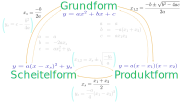
\includegraphics[width=15cm]{allg/funktionen/img/formen/formen.png}
\end{center}

\begin{bemerkung}{}{}
  Das $a$,  ist in allen Formen derselbe Wert und bestimmt die Parabelöffnung.
  \end{bemerkung}
\newpage

\textbf{Grundform aus Scheitelform} (einfaches Ausmultiplizieren). Beispiel:
$$y=2(x-3)^2-4 = 2(x^2-6x+9)-4=2x^2-12x+14$$

\begin{tabular}{rcl}
$a(x-x_S)^2+y_S$ &=& $ax^2-2ax_Sx + (ax_S^2+y_S)$\\
  $a$ &=& $a$ \\
  $b$ &=& $-2ax_S$\\
  $c$ &=& $ax_S^2+y_S$
\end{tabular}


\textbf{Grundform aus Produktform} (einfaches Ausmultiplizieren). Beispiel
$$y=2(x+3)(x-4)=2(x^2 +(3-4)x - 12) = 2x^2-x-24$$

\begin{tabular}{rcl}
  $a(x-x_1)(x-x_2)$ &=& $ax^2 - a(x_1+x_2)x + ax_1x_2$\\
  $a$ &=& $a$ \\
  $b$ &=& $-a(x_1+x_2)$\\
  $c$ &=& $ax_1x_2$
\end{tabular}


\textbf{Nullstellenform (Produktform) aus Grundform}:
Gegeben: $y = ax^2 + bx + c$

Nullstellenform: $y = a(x-x_1)\cdot{}(x-x_2)$ mit

$$x_{1,2} = \frac{-b \pm \sqrt{b^2-4ac}}{2a}$$

\begin{beispiel}{}{}
Gegeben $y = 5x^2 - 5x - 30$. Schreiben Sie dies in der Produktform (=
Nullstellenform):
\platzFuerBerechnungen{3.2}\TRAINER{$y = 5(x-3)(x+2)$\vspace{4.2cm}}
\end{beispiel}
\newpage


\textbf{Scheitelform aus Grundform}:
$$x_S=\frac{-b}{2a}$$

$y_S$ einfach durch Einsetzen von $x_S$ in die Grundform:
$$y_S=c-\frac{b^2}{4a}$$
 
\textbf{Scheitelform aus Produktform}: $x_S$ ist der Mittelwert der beiden
Nullstellen:
$$x_S=\frac{x_1+x_2}{2}$$
Danach $y_S$ einfach durch Einsetzen von $x_S$ in die Produktform:
$$y_S=\frac{-a}{4}(x_1-x_2)^2$$

\textbf{Produktform aus Scheitelform}: Einfachster Weg geht über die Grundform oder abgekürzt:
$$x_{1,2} =x_S \pm \sqrt{\frac{-y_S}{a}}$$


\subsection{Aufgaben}

\TALS{\olatLinkArbeitsblatt{Umrechnen der Formen}{https://olat.bbw.ch/auth/RepositoryEntry/572162090/CourseNode/103176133021102}{1., 2., 3. und 8.}}



\newpage

% Bereits in typ I II und III eingebaut
%\subsection{Parabel aus drei Punkten}
Vorzeigeaufgabe Marthaler Algebra S. 272 Aufg. 3. b) 


\subsection*{Aufgaben}

\AadBMTA{272}{3. a) c)}%% war Marthaler S. 187 Aufg. 676 a) und b)
\GESOAadBMTA{???}{???}

\newpage



%\newpage

%

%%%%%%%%%%%%%%%%%%%%%%%%%%%%%%%%%%%%%%%%%%%%%%%%%%%%%%%%%%%%%%%%
\subsection{Extremwertaufgaben}



\subsubsection{Aus alter Maturprüfung}

\aufgabenFarbe{Gegeben ist die Funktion $f(x) = x\cdot{}(3-\sqrt{x})$,
  $x\in[0;\infty[$.\\
  a) Bestimmen Sie die Nullstellen und das  Extremum der Funktion
  $f$.\\
  b) Im ersten Quadranten, zwischen dem  Graphen und der
  $x$-Achse ist ein  rechtwinkliges Dreieck $ABC$ einbeschrieben.  Der
  rechte Winkel ist in der Ecke $B$.  Punkt $A$ liegt im Ursprung, $B$
  auf der  $x$-Achse und $C$ auf dem Graphen von $f$. Berechnen Sie
  die Koordinaten des  Punktes $C$ so, dass der Flächeninhalt des
  Dreiecks maximal wird.
}%% END aufgabenFarbe

    
\bbwCenterGraphic{8cm}{tals/fct3/img/Maximieren.png}
\TNTeop{
   a) solve$(f(x)=0,x)$ Somit sind die Nullstellen bei 0 und 9\\
     $\text{fmax}(f(x),x)$ liefert $x=4$ ist Maximalstelle (und auch
     Maximalwert ($f(4)=4$)\\
   b) $\text{fmax}(0.5\cdot{}x\cdot{}f(x), x)$ liefert $x = 5.76$ und
   $f(5.76) = 3.456$}%% End TNTeop
\newpage
\subsection*{Aufgaben}
\AadBMTA{311}{49.}
\AadBMTA{321}{17.}

%\newpage

\section{Berührende Graphen}\index{Graphen!berührende}\index{berührende Graphen}

\textbf{Einführungsbeispiel}


Gegeben ist die Parabel $f: y=\frac{1}{4}x^2 -\frac12x +\frac14$ und von einer
Geraden $g$ ist der $y$-Achsenabschnitt $b = -2$ gegeben.

Gesucht ist von der Geraden $g$ die Steigung $a$ so, dass die
Gerade die Parabel tangiert; also genau in einem Punkt berührt.

Wo (in welchem Punkt $B=(x_B|y_B)$) tangiert also die Gerade $g$ die Parabel $f$?

In der folgenden Skizze sind drei mögliche Geraden mit $y$-Achsenabschnitt
$-2$ gezeichnet. Nur eine dieser drei Geraden \textit{tangiert} die Parabel.

\bbwGraph{-4}{4}{-3}{5}{
  \draw[thick,color=blue,variable=\x,domain=-3.5:4] plot ({\x},   {0.25*\x*\x -0.5*\x + 0.25});

  \draw[color=red,variable=\x,domain=-3:5] plot ({\x},{2*\x -2});
  \draw[color=red,variable=\x,domain=-3:5] plot ({\x},{0.5*\x - 2});
  \draw[color=cyan,thick,variable=\x,domain=-3:5] plot ({\x},{1*\x  -2});

  \bbwDot{3, 1}{green}{north}{B}

  %%%\draw[thick,color=blue,variable=\x,domain=-1:5] plot ({\x}, {0.5*\x*\x - 2*\x + 3}); 
  %%\draw[color=red,variable=\x,domain=-1:5] plot ({\x},{0.5*\x + 1});
  %%\draw[color=red,variable=\x,domain=-1:5] plot ({\x},{0.5*\x - 1.5});
  %%\draw[color=cyan,thick,variable=\x,domain=-1:6] plot ({\x},{0.5*\x  -0.125});
  %%\bbwDot{2.5, 1.125}{green}{north}{P}
}
\newpage
\textbf{Lösungsidee}: Der gesuchte Parameter ist $a$, die Steigung der
Geraden.

Nun berechne die Schnittpunkte/den Schnittpunkt mit $$f(x) = g(x).$$

Das $a$ ist gefunden, sobald die Gleichung $f(x)=g(x)$ genau eine
Lösung aufweist; dann also, wenn


\TNT{2}{die Diskriminante dieser Gleichung
verschwindet.}

Den $x$-Wert dieses Berührungspunktes nennen wir $x_B$:


Ansatz:

$$f(x_B) = g(x_B)$$

\TNT{4.4}{
 
\begin{tabular}{rclr}
$\frac14x_s^2-\frac12x_s+\frac14$          & $=$ &  $ax_s-2$ & \\
$\frac14x_s^2+(-\frac12-a)x_s + \frac94$   & $=$ & $0$       & (I)\\
\end{tabular}
\vspace{10mm}
}%% END TNT

Die Diskriminante $D=B^2 - 4AC$ muss gleich 0 sein. 

\TNT{7.2}{
$A = \frac14$, $B = -\frac12-a$ und $C = \frac94$.

  $$D=0=B^2-4AC = (-\frac12-a)^2  - (4\cdot{}A\cdot{}C)$$
  $$0 = (a^2+a+\frac14) - (4\cdot\frac14\cdot{}\frac{+9}4)$$
$$\Longrightarrow 0 = a^2 + a - 2$$
$$\Longrightarrow a_1 = 1 \text{ und  } a_2 = -2$$
\vspace{40mm}
}%% END TNT
\newpage

Für den \textbf{Berührungspunkt} $B=(x_B|y_B)$ müssen wir nun nur doch das gefundene
$a$ in die Gleichung (I) einsetzen.


\TNT{6}{
  $$0 = \frac14x_B^2 + (-\frac12 -a ) + \frac94$$

  $$x_B = x_1 = x_2 = \frac{-B \pm\sqrt{D}}{2A} = \frac{-B \pm
    \sqrt{0}}{2A} = \frac{-B}{2A}$$

  $$x_B = \frac{-B}{2A} = \frac{- (-\frac12 - a)}{\frac24} =
  \frac{\frac12 + a}{\frac12} = (\frac12 + a) : \frac12 = (\frac12+a)
  \cdot{} 2 = 1+2a$$
}



1. Fall: ($a_1=1$):

\TNT{6}{
$B_1: a_1 = 1:$
  $$x_B = 1+2a = 1 + 2\cdot{}(1) = 3$$

Das $y$ finden wir einfach durch Einsetzen von $x$ in den
Funktionsterm der Geradengleichung.

$$y_1 = a_1x_1 - 2 = 1\cdot{}3-2 = 1$$
und somit ist
$$B_1 = (3 | 1)$$
}%% END TNT



2. Fall: ($a_1=-2$):


\TNTeop{
$B_2: a_2 = -2:$
  $$x_B = 1+2a = 1 + 2\cdot{}(-2) = 1-4=-3$$


$$y_2 = a_2x_2+b = -2\cdot{}3-2 = 4$$
und somit ist
$$B_2 = (-3 | 4)$$

}%% END TNT
\newpage




\begin{rezept}{Berührende Graphen}{}

  Bei Berührungsaufgaben mit Parabeln hilft i.\,d.\,R. das folgende
  Vorgehen:

  \begin{enumerate}
  \item Funktionsterme Gleichsetzen: $$f(x) = g(x)$$
  \item In Grundform bringen: $$f(x) - g(x) = 0  \hspace{40mm}
    (I)$$
  \item Diskriminante $D = 0 $ setzen, um den Parameterwert zu
    bestimmen.
  \item Gleichung $(I)$ auflösen mit dem Wissen $D=0$.
    $$x_B=x_1=x_2= \frac{-B}{2A}$$

  \item Gefundenen Parameter in $x_B=\frac{-B}{2A}$ einsetzen, um $x$
    des Berührungspunktes zu bestimmen.
  \item Das $y_B$ des Berührungspunktes ermitteln, indem wir $x_B$ in
    $f$ oder $g$ einsetzen.
    \end{enumerate}
\end{rezept}


\TRAINER{(Je nach Zeit wäre 699. a) noch eine Vorzeigeaufgabe.)}

\subsection{Aufgaben}
\TRAINER{Achtung, dass nicht das Gleichungssystem bereits
  nach dem Gleichsetzen der Graphen aufgestellt wird. Erst nach dem
  Null-Setzen der Diskriminante erhalten wir eine gültige Gleichung
  für das Gleichungssystem.}
%%\TALSAadBMTA{190}{698., 702., 703., 705.}
\TALSAadBMTA{277}{30. a), 36. a), 40. a) c), 42. a), 43. a), 44. a)}
\newpage


\subsection{Grenzwerte und Steigungsfunktion (Optional)}

Wie macht das ein CAS, dass es den tiefsten bzw. den höchsten Punkt
einer Funktion bestimmen kann? Hier ein Erklärungsversuch am Beispiel
der quadratischen Funktion.
Betrachten wir die allgemeine quadratische Funktion $$p: y=ax^2 + bx +
c$$
Mit dem selben $a$ und dem selben $b$ kann ich eine Gerade $s$
definieren, die ich die (Tangenten-)\textbf{Steigungsfunktion}\footnote{Diese
  Steigungsfunktion wird in der Mathematik die
  \textbf{Ableitung}\index{Ableitung} genannt. Genau genommen handelt
  es sich nicht um die Steigung der Parabel, sondern um die Steigung
  einer im Punkt $P=(X_P|f(x_P))$ angelegter Tangente.} nenne:
$$s: y= 2ax+b$$
\newpage


Diese Steigungsfunktion $s$ gibt in jedem Punkt $x$ die Steigung einer
Tangente an die Parabel $p$ an.

\begin{beispiel}{Parabel}{}
  Gegeben ist die Parabel $$p: y=2.5x^2 - 3x + 6.5\text{.}$$

  Wo (für welches $x$) hat diese Parabel
  ihren Tiefpunkt? \TRAINER{Scheitelpunkt:}

  $$x_B =   \LoesungsRaumLen{8cm}{\frac{-b}{2a} = \frac{-(-3)}{2\cdot{}2.5} = 0.6}$$

  Dies ist gleichzeitig die Nullstelle der
  Steigungsfunktion:

  $$s: y= \LoesungsRaumLen{3cm}{2\cdot{}2.5x - 3}$$

  Nullstelle von $s$:

  $$x_0 = \LoesungsRaumLen{7cm}{\frac{3}{2\cdot{}2.5} = 0.6}$$

  Wir können damit aber auch die Steigung in einem ganz anderen Punkt
  \zB für $x=10$ berechnen. Die Parabel $p$ hat an der Stelle $x=10$
  die Tangentensteigung, die durch die Steigungsfunktion im Punkt $10$
  ermittelt wird:

  $$s(10) = \LoesungsRaumLen{40mm}{2\cdot{}10\cdot{2.5} - 3 = 47}$$
  
\end{beispiel}
\newpage

\begin{beispiel}{Gerade gesucht}{}
Gegeben ist die Parabel $$p: y=4x^2 -6x + 3\text{.}$$ Gesucht ist die Gerade
$g: y=ax+b$, sodass die Gerade die Parabel bei $x=7$ berührt.

\begin{enumerate}
\item Die Steigungsfunktion $s$ lautet: $$s:
  y=\LoesungsRaumLen{5cm}{2\cdot{}4x - 6}$$
  
\item Für $x=7$ hat die Steigungsfunktion den Wert \LoesungsRaumLen{1cm}{50}, und somit hat
  die Parabel bei $x=7$ die Steigung \LoesungsRaumLen{1cm}{50}.

  
\item Um den Berührungspunkt $B$ zu finden, setzen wir 7 diesen in $p$
  ein
  $$p(7)= \LoesungsRaumLen{5cm}{4\cdot{}49-6\cdot{}7+3 = 157}$$
  und somit ist
  $$B=(\LoesungsRaum{7}|\LoesungsRaum{157})$$
  
\item Die gesuchte Gerade $g: y=ax+b$ hat also auch die Steigung \LoesungsRaum{50}
  und verläuft durch den Berührungspunkt $B=(\LoesungsRaumLen{9mm}{7}|\LoesungsRaumLen{11mm}{157})$. Also
  $$\LoesungsRaumLen{7cm}{157=50\cdot{}7+b}$$

  Somit ist das gesuchte
  $$b = \LoesungsRaumLen{55mm}{157-50\cdot{}7=-193}$$
  
  und die gesuchte Funktionsgleichung der Geraden lautet: $$y = \LoesungsRaumLen{22mm}{50x-193}$$
  \end{enumerate}
\end{beispiel}

\TRAINER{Idee: Auf mm-Papier eine Funktion $y=\frac1{27}x^3-\frac19
  x^2 - \frac89 x$ vorgeben.

Auftrag: Legen Sie in 5 Punkten eine Tangente an die Funktion und
bestimmen Sie deren Steigung.
Tragen Sie die Steigung in ein neues Koordinatensystem ein: $x$-Achse
= $x$ Wert, $y$-Achse = Steigung der Funktion.
$$f' : y = \frac19 (x-1)^2 - 1 $$
}%%
\newpage

\subsubsection{Beweis der Formel der (Tangenten-)Steigungsfunktion}

Betrachten wir auf auf der $x$-Achse zwei benachbarte Punkte $x$ und
$x+\Delta$. Die Funktionswerte lauten $f(x)$ und $f(x+\Delta)$. Die
\textbf{Steigung} kann nun für eine Gerade bestimmt werden durch:

\bbwCenterGraphic{7cm}{tals/fct3/img/Steigungsfunktion.jpg}

$$\frac{f(x+\Delta) - f(x)}{\Delta}$$

Dies gilt für eine Parabel $p: y=ax^2+bx+c$ näherungsweise auch:
$$\frac{f(x+\Delta)-f(x)}{\Delta} = \frac{(a(x+\Delta)^2 + b(x+\Delta)
  + c) - (ax^2 + bx +c)}{\Delta}=2ax+a\Delta+b$$

Wenn wir nun das $\Delta$ gegen Null gehen lassen, also immer kleinere
Werte einsetzen, so verschwindet der Term $a\cdot{}\Delta$ fast und unsere
Formel stimmt annähernd --- jedoch präzise genug, um dies als Beweis
gelten zu lassen.

Ein anderer Beweis wäre die Tangente effektiv einzusetzen und diese so
zu wählen, dass es genau einen Schnittpunkt gibt, was wieder darauf
zurückführt, dass die Diskriminante = Null gesetzt werden muss. Dann
sind wir exakt, aber der Beweis ist ungleich aufwändiger.
\newpage


\newpage



%% Datenanalyse
%%%%%%%%%%%%%%%55
%% Funktionen II TALS Metapackage
\part{Funktionen II}\index{Funktionen!II|textbf}
\renewcommand{\bbwPartID}{FCT2}
%%
%% 2019 07 04 Ph. G. Freimann
%%

\section{Quadratische Funktionen}\index{Funktionen!quadratische}
\sectuntertitel{Geraden im Lande der Parabeln wird dringend angeraten, einen
  Integrationskurs zu besuchen.}
%%%%%%%%%%%%%%%%%%%%%%%%%%%%%%%%%%%%%%%%%%%%%%%%%%%%%%%%%%%%%%%%%%%%%%%%%%%%%%%%%

%%\bbwCenterGraphic{8cm}{tals/fct2/img/lugano2018.jpg}
%%\textit{Bildlegende: Parabeln in Lugano (2018)}
\bbwCenterGraphic{175mm}{tals/fct2/img/paris2022.jpg}
\textit{Bildlegende: Parabeln in den Gärten von Versailles (2022)}

\subsection*{Lernziele}

\begin{itemize}
\item Definition
\item Formen: Scheitel-, Produkt-, Normalform
\item Graphische Darstellung
\item Translationen und Spiegelungen
\end{itemize}

\TadBMTA{260}{15}
%%\TALS{(\cite{frommenwiler17alg} S.183 (Kap. 3.4))}
%%\GESO{(\cite{marthaler21alg}       S.260 (Kap. 15))}

Einstieg: Bilder von Heimgartner/Hunziker.


\textbf{Einstiegsaufgabe: } \aufgabenFarbe{Lösen Sie Aufgaben 1. und 2.
  von Seite 272: Welche der angegebenen Funktionen sind quadratisch?}

\newpage

\subsection{Parabel}\index{Parabel}\index{Normalparabel}

Zeichnen Sie die Funktionen $f: y=x^2$ (= Normalparabel), $y=\frac{1}{3}x^2$

und $y=-0.25\cdot{}x^2$  ins Koordinatensystem:

\bbwGraph{-3}{3}{-3}{7}{
  \TRAINER{\bbwFuncC{\x * \x}{-2.5:2.5}{green}
    \bbwFuncC{-0.25*\x * \x}{-3:3}{green}
    \bbwFuncC{\x * \x / 3}{-3:3}{green}
  }
}


\newpage

\subsection{Grundform}\index{Grundform!quadratische Funktion}\index{Quadratische Funktion!Grundform}
Die Funktion $f(x): x \mapsto y = ax^2 + bx +c$ ist eine
quadratische Funktion in Grundform\index{Grundform!quadratische Funktion}.

Spielen Sie mit \TALS{dem TI-nSpire oder mit} \texttt{geogebra.org} an den Parametern $a$, $b$ und $c$ der Funktionsgleichung $y = a\cdot{}x^2 + b\cdot{} x + c$ herum. Was bewirkt der Parameter

$a$: \LoesungsRaumLang{Parabelöffnung: $|a|$ klein: Breite (weite) Öffnung / $|a|$ groß: Enge, schmale Öffnung. $a < 0$: Parabel ist nach unten geöffnet. $a > 0$: Parabel ist nach oben geöffnet.}

$b$: \LoesungsRaumLang{«Parabelsteigung»\footnote{Mit «Parabelsteigung» ist hier die Steigung der entsprechenden Tangente gemeint.} im Punkt $A(0|c)$}

$c$: \LoesungsRaumLang{$y$-Achsenabschnitt. Damit wird eine Verschiebung der Parabel entlang der $y$-Achse erreicht.}

Versuchen Sie eine Parabel mit Scheitelpunkt $(1|1)$ zu finden\TRAINER{(Lösung: $b=-2a$ und $a+b+c=1$.)}.

\subsection*{Aufgaben}
%%\TALSAadBMTA{184ff}{660. a) c) f), 662. a) b) c) und e)}
\AadBMTA{273}{5., 6., 7., 8. und 9.}
\newpage

\subsection{Vier charakteristische Punkte}
Zeichnen Sie die Funktion
$$p: y = x^2 - 4x + \frac{7}{4}$$

\bbwGraph{-3}{6}{-3}{2}{
\TRAINER{\bbwFunc{\x*\x - 4*\x + 1.75}{-0.2:4}}
}%% end BBW Graph

Wo befinden sich die charakteristischen Punkte?

\TNT{2.4}{\vspace{24mm}}


Die charakteristischen Punkte sind:
\begin{itemize}
\item Schnittpunkt mit $y$-Achse = (\LoesungsRaum{0} | \LoesungsRaum{1.75})
\item Nullstellen: $N_1=(\LoesungsRaum{0.5}| \LoesungsRaum{0}), N_2=( \LoesungsRaum{3.5}|\LoesungsRaum{0})$
\item Scheitelpunkt: $S=(\LoesungsRaum{2}|\LoesungsRaum{-2.25})$
\end{itemize}
 
Wie berechnen sich nun diese Punkte?
\newpage
\subsubsection{Parabelöffnung}
Eigentlich ist die Parabelöffnung kein charakteristischer
Punkt. Dennoch kann man eine $x$-Einheit vom Scheitelpunkt entfernt,
das $a$ der Grundform ($y=ax^2+bx+c$) direkt ablesen. Gehen wir bei
der Normalparabel ($a=1$) vom
Scheitelpunkt um eine Einheit nach rechts, so muss die Parabel um eine
$y$-Einheit nach oben anwachsen.

\TNT{10}{
Parabel durch Scheitelpunkt $P=(-3|1)$ und durch $(-2|2)$ =
verschobene Normalparbel zeichnen.

Parabel mit Scheitelpunkt $P=(2|2)$ durch $(3|0.5)$ zeichnen. Das $a$
ist somit sofort $a=-1.5$ abzulesen.
}

\subsubsection{$y$-Achsenabschnitt}
Genau wie bei der linearen Funktion, gilt für den $y$-Achsenabschnitt,
dass die $x$-Koordinate dieses Punktes Null ist.
$$y = x^2 -4x + 1.75$$
wird mit $x=0$ zu
$y = 1.75$.

Der $y$-Achsenabschnitt ist somit immer das $c$ aus $y = ax^2 + bx +
c$.

\newpage

\subsubsection{Nullstellen}
Wie bei den linearen Funktionen sind auch hier die
Nullstellen die Schnittpunkte mit der $x$-Achse. Dies bedeutet für die
Nullstellen $N(x_0 | y_0)$, dass die $y$-Koordinate = 0 ist. Es gilt
also

$$0 = x^2 - 4 x + \frac{7}{4} $$

Dies ist eine quadratische Gleichung mit den Lösungen:

$$x_{1,2} = \frac{-b \pm \sqrt{b^2-4ac}}{2a}$$ 

\noTRAINER{\platzFuerBerechnungen{2.4}}
\TRAINER{$x_{1} = 0.5; x_{2}=3.5$ (Mitternachtsformel)
  \vspace{3cm}}

\begin{bemerkung}{}{}
  Die Nullstellen der quadratischen Funktion entsprechen den Lösungen
  der zugehörigen quadratischen Funktion (mit $y=0$). Daher gilt
  auch hier: 


  \begin{tabular}{c|p{8cm}}
    Diskriminante $D=b^2-4ac$ > 0 & Es gibt zwei Nullstellen. \\
    \hline\\
    Diskriminante $D=b^2-4ac$ = 0 & Es gibt eine Nullstelle, denn der Scheitelpunkt liegt auf der $x$-Achse.\\
    \hline\\
    Diskriminante $D=b^2-4ac$ < 0 & Es gibt keine Nullstellen, denn die Parabel schneidet die $x$-Achse nicht.\\
  \end{tabular}
  
 \ifisALLINONE{Zum Begriff \textbf{Diskriminante}:  \totalref{diskriminante}}\fi{} 
\end{bemerkung}

\subsection*{Aufgaben}
\AadBMTA{277ff}{28. a) c) }

\newpage



\subsubsection{Scheitelpunkt}\index{Scheitelpunkt}
Der Tief- bzw. Hochpunkt einer Parabel wird \textbf{Scheitelpunkt}
genannt.

Wir berechnen den Scheitelpunkt in zwei Schritten.

\textbf{Erstens:} Wir berechnen den Mittelwert der beiden Nullstellen:
$$x_S := \frac{x_{1} + x_{2}}{2} = \frac{\frac{-b+\sqrt{D}}{2a} + \frac{-b-\sqrt{D}}{2a}}{2} =
\frac{(-b+\sqrt{D}) + (-b-\sqrt{D})}{4a} =\frac{-b}{2a}$$
Dabei ist $D$ die Diskriminante $D=b^2-4ac$.

\platzFuerBerechnungen{2.4}
\TRAINER{$x_S = 2$
\vspace{3cm}}

\textbf{Zweitens:} Wir setzen den gefundenen $x$-Wert
(\LoesungsRaum{2}) in die Funktionsgleichung
ein:
$$y_S = x^2 - 4x + 1.75$$
$$y_S = (\LoesungsRaum{2})^2 - 4\cdot{}(\LoesungsRaum{2}) + 1.75$$

Wir erhalten für den Scheitelpunkt $S$: $S=(x_S | y_S) = (\LoesungsRaum{2} | \LoesungsRaum{-2.25})$.

\begin{gesetz}{Scheitelpunkt}{}
  Der Scheitelpunkt $S$ einer Parabel in der Grundform ($y=ax^2+bx+c$) kann wie folgt
  berechnet werden:

  $$S=\left(\frac{-b}{2a}\middle|\frac{4ac-b^2}{4a}\right)$$

  (Bem.: Der $y$-Wert kann einfach durch Einsetzen des $x$-Wertes in
  die Funktionsgleichnug gefunden werden.)
  \end{gesetz}
  
\subsection*{Aufgaben}
%%\TALSAadBMTA{184ff}{665. a) b) c) 666. a) b) c) e) f) g)}
\AadBMTA{273}{4. (=Aufg. 22. S. 276)}

\newpage

\subsection{Bestimmen der Funktionsgleichung}
\TALS{S. 187 Kap. 3.4.3}

\subsubsection{Referenzaufgaben}

\textbf{TYP I}

Gegeben ist ein Punkt $P$ mit den Koordinaten $(2.3 | -1.5)$. Gesucht ist die reinquadratische Funktion $f: y=a\cdot{}x^2$, welche durch diesen Punkt geht.
Machen Sie vorab eine Skizze.

\bbwGraph{-3}{3}{-2}{1}{
  \TRAINER{\bbwFunc{-0.2836 * \x * \x}{-2.5:2.5}
    \bbwDot{2.3,-1.5}{blue}{west}{P}
  }%% end TRAINER
}%% end BBW Graph

\platzFuerBerechnungen{3.6}

\TRAINER{Idee: Punkt einsetzen: $-1.5 = a\cdot{}(2.3)^2$. Das Auf"|lösen dieser Gleichung liefert $a = \frac{-1.5}{2.3^2}$. Dies liefert $a\approx -0.2836$}

Weitere «TYP 1» Aufgaben wären z. B. $y = 3x^2 - bx + 4$ oder $y=2x^2
-7x + c$ mit anderen Worten alle Parabeln mit genau \textbf{einem}
Parameter, daher «Typ 1».

\newpage



\textbf{TYP II}

Gegeben sind zwei Punkte und wir haben zwei Unbekannte.

\begin{rezept}{}{}
  Gesucht sind $a$ und $c$ aus $y = ax^2 + c$ bei den gegebenen
  Punkten $(7|5)$ und $(2|-4)$.

  Wir lösen dies auch durch Einsetzen der Punkte in die
  Funktionsgleichung und wir erhalten zwei Gleichungen:


  \begin{tabular}{c | r  c  r |}
    (I)  &  $5$ & = & $(7)^2\cdot{} a + c$ \\
    (II) & $-4$ & = &  $(2)^2\cdot{} a + c$ \\
  \end{tabular}

  Durch Subtrahieren der Gleichungen erhalten wir

  \begin{tabular}{c | r  c  r | c}
    (I)  &  $5$ & = & $49\cdot{} a + c$ & \,\\
    (II) & $-4$ & = &  $4\cdot{} a + c$ & $\ominus$\\
  \end{tabular}

  $$9 = 45a$$ und somit
  $$a =\frac{1}{5}.$$

  Dieses $a$ (= $\frac{1}{5}$) setzen wir nun in eine der Gleichungen
  (\zB (I)) ein und erhalten
  $$5=49\cdot{}\frac{1}{5} + c$$
  und nach Auf"|lösen erhalten wir $c=\frac{-24}{5}$.

  Die gesuchte Gleichung lautet also:

  $$y = \frac{1}{5}x^2 - \frac{24}{5}$$
\end{rezept}

Probe durch Einsetzen der $x$-Werte der Punkte in die gefundene Funktionsgleichung:

\TNTeop{}
%%\newpage

\begin{beispiel}{}{}
  Anstelle von $a$ und $c$ können natürlich auch $a$ und $b$ gesucht
  sein. Daher eine zweite Aufgabe.

  Gesucht sind $a$ und $b$ aus $y = ax^2 + bx$ bei den gegebenen

  Punkten $(2|-6)$ und $(-3|5)$.

  Wir lösen dies wiederum durch Einsetzen der Punkte in die
  Funktionsgleichung und wir erhalten die beiden Gleichungen, welche
  wir durch das Additionsverfahren lösen können:

  \begin{tabular}{c | r  c  r | c}
    (I)  &  $-6$ & = & $4a + 2b$ & $\cdot{} 3$ \\
    (II) &   $5$ & = & $9a - 3b$ & $\cdot{} 2$ \\
  \end{tabular}

  somit:
  
  \begin{tabular}{c | r  c  r | c}
    (I')  & $-18$ & = & $12a + 6b$ &\, \\
     \,   & \,    & \,&   \,       & $\oplus$\\
    (II') &  $10$ & = & $18a - 6b$ &\, \\
  \end{tabular}

  Nach Addition der Gleichungen erhalten wir

  $$-8 = 30a$$

  was uns zu $a=\frac{-4}{15}$ bringt.

Dieses $a$ können wir nun wieder in eine der beiden Gleichungen
einsetzen (\zB in (I)):

$$-6=4\cdot{}\frac{-4}{15} + 2b$$

Das Auf"|lösen obiger Gleichung liefert nach Kürzen: $b=\frac{-37}{15}$.

Die gesuchte Funktionsgleichung lautet also

$$y = \frac{-4}{15} x^2 - \frac{37}{15} x.$$

\end{beispiel}

Auch bei «Typ II» kann natürlich jede \textbf{zwei}parametrige quadratische
Funktion herhalten, wie \zB $y=-6cx^2 + bx - c$ durch \textbf{zwei}
gegebene Punkte.
\newpage


\textbf{TYP III}: Gegeben sind hier drei Punkte, wir haben aber auch
drei Unbekannte in $y = ax^2 + bx + c$. Die Punkte sind hier
(1|3), (2|3.5) und (-3|11).

Durch Einsetzen der drei Punkte je in die Funktionsgleichung erhalten
wir drei Gleichungen:

\begin{tabular}{c|r c rcrcr|}
  (I)   & 3   & = & $(1)^2\cdot{}a$  &$+$& $(1)\cdot{}b$  &$+$& c \\ 
  (II)  & 3.5 & = & $(2)^2\cdot{}a$  &$+$& $(2)\cdot{}b$  &$+$& c \\ 
  (III) & 11  & = & $(-3)^2\cdot{}a$ &$+$& $(-3)\cdot{}b$ &$+$& c \\ 
\end{tabular}

Vereinfachen:

\begin{tabular}{c|r c rcrcr|}
  (I)   & 3   & = & $a$  &$+$& $b$  &$+$& c \\ 
  (II)  & 3.5 & = & $4a$ &$+$& $2b$ &$+$& c \\ 
  (III) & 11  & = & $9a$ &$-$& $3b$ &$+$& c \\ 
\end{tabular}

Nun finden wir $a$, indem wir zunächst $c$ durch Subtraktion
eliminieren:

\begin{tabular}{l|r c rcr|}
  (IV) = (II) -   (I) & 0.5  & = & $3a$ &$+$& $b$ \\ 
  (V)  = (III) - (II) & 7.5  & = & $5a$ &$-$& $5b$ \\ 
\end{tabular}

Multiplizieren wir nun die Gleichung (IV) mit 5, so erhalten wir

\begin{tabular}{r|r c rcr|}
  5$\cdot{}$(IV)  & 2.5  & = & $15a$ &$+$& $5b$ \\ 
  (V)             & 7.5  & = & $5a$  &$-$& $5b$ \\ 
\end{tabular}

Durch Addition der beiden Gleichungen (IV) und (V) erhalten wir

$10 = 20a$ oder $a = \frac{1}{2}$.

Um $b$ zu finden, setzen wir $a = \frac{1}{2}$ in (V) ein: $7.5 =
5\cdot{}\frac{1}{2} - 5b$.

Auf"|lösen nach $b$ ergibt $b = -1$.

Zu guter Letzt setzen wir $a = \frac{1}{2}$ und $b=-1$ in die
Gleichung (I) ein, um noch $c$ zu erhalten:

$$3 = a + b + c = \frac{1}{2} - 1 + c$$

Somit ist $c=3.5$ und die Funktionsgleichung lautet:

$$y = \frac{1}{2}x^2 - x + 3.5$$


\TALS{\subsection*{Aufgaben}}
%%\TALSAadBMTA{187ff}{676. a) c), 682., 684.}
\AadBMTA{272}{3. a) c), 20. a) c), 21., 22., 24. a), 25. b)}
\newpage


\subsection{Computer Algebra Systeme (CAS)}\index{CAS}
Das eben gezeigte Beispiel wird in der Praxis meist nicht von Hand,
sondern mit einem Computer-Algebra-System, kurz CAS, gelöst:

\paragraph{Aufgabenstellung}
Gegeben sind wieder drei Punkte (1|3), (2|3.5) und (-3|11).
Gesucht ist die Parabel $y = ax^2 + bx + c$, welche durch die drei
Punkte geht.

Dies wird mit dem \tinspire{} wie folgt gelöst:
\begin{itemize}
\item Definiere die Funktionsgleichung mit
  Parametern\footnote{\tinspire Regel: $ax\ne a\cdot{} x$}:\\
  $$f(x) := a\cdot{}x^2 + b\cdot{}x + c$$
\item Definiere das Gleichungssystem:
  $$gls := \left\{ \begin{array}{l}
    f(1) = 3\\
    f(2) = 3.5\\
    f(-3)= 11\\
  \end{array}\right.$$
\item Löse das Gleichungssystem:
  $$solve(gls,\{a, b, c\})$$
\end{itemize}

\subsection*{Aufgaben}
\AadBMTA{272}{3. b) d)}

\newpage

\subsection{Formen der quadratischen Funktion}
\subsubsection{Nullstellenform}\index{Nullstellenform}

Die \textbf{Nullstellenform} wird auch  «faktorisierte Form» oder
«Produktform» genannt.\index{faktorisierte Form}\index{Produktform}

Beachten Sie die folgende quadr. Funktionsgleichung:

$$y = 3.1(x-5)(x+6)$$

Dies ist eine quadratische Funktion in der sogenannten
\textbf{Nullstellenform}, denn die Nullstellen (hier $x_0 = 5$ oder
$x_0 = -6$) können direkt aus der Funktionsgleichung abgelesen werden.
Wenn wir $y=0$ in die Gleichung setzen (Nullstelle),

$$0 = 3.1(x-5)(x+6)$$
so wird die Gleichung genau dann wahr, wenn (mind.) einer der beiden Klammerausdrücke rechts
gleich Null ist. Die Parabelöffnung (hier 3.1) kann dabei beliebig variieren und ist (neben den Nullstellen) der einzige Parameter.

Die Nullstellenform lautet

\begin{gesetz}{}{}

  $$y = a(x-x_1)\cdot{}(x-x_2)$$

  \end{gesetz}

wobei $x_1$ und $x_2$ die Nullstellen der Parabel bezeichnen. 
\newpage


\subsubsection*{Referenzaufgabe zur Nullstellenform}

\noTRAINER{\bbwGraphic{16cm}{tals/fct2/img/BrunnenNullstellenformOhneKoordinatensystem.png}}
\TRAINER{\bbwGraphic{16cm}{tals/fct2/img/BrunnenNullstellenformMitKoordinatensystem.png}}

Ein parabelförmiger Wasserstrahl spritzt ebenerdig aus einem Brunnen und trifft 7m von der Düse entfernt wieder auf dem Boden auf.
Das Wasser steigt also erst gleich hoch an, wie es danach wieder «herunterfällt».
Dabei wird gemessen, dass 1m von der Düse entfernt der Wasserstrahl 84cm über Boden verläuft.
Können Sie aufrecht unter dem Wasserstrahl hindurchgehen?

Tipp: Skizze und  die Parabelgleichung in Nullstellenform aufschreiben. Die Düse ist der Ursprung der Koordinatensystems.\\

\TNT{5.2}{Die Funktionsgleichung lautet $y=a(x-x_1)(x-x2)$.\\
  Mit den Nullstellen $x_1=0$ und $x_2=7$.\\
  Wir setzen den gemessenen Punkt (1|0.84) in die Gleichung ein und erhalten $0.84 = a\cdot{}(1-0)(1-7)$.\\
  Daraus ergibt sich $a=0.84/(-6) = -0.14 $.\\
  Nun setzen wir 3.5 Meter in die Funktionsgleichung $y = -0.14(x-0)(x-7)$ ein: und erhalten $y=-01.4\cdot{}3.5\cdot{}(-3.5) = 1.715m$; das ist die höchste Parabelstelle.}


\subsection*{Aufgaben}%% Nullstellenform
%%\TALSAadBMTA{185}{663, 678., 680.}
\TALSAadBMTA{277}{30. a) b), 31. b)}
\newpage

%%\TRAINER{\, \newpage}
\subsubsection{Scheitelform}\index{Scheitelform!der quadratischen
  Funktion}
Einstieg: Wo hat die Parabel $f: y=3.6(x-4)^2 + 5$ ihren
Scheitelpunkt?

\TNT{4.4}{CAS: bei $x_S = 4$ und $y_S= 5$; völlig irrelevant ist die 3.6.}

Ist eine quadratische Funktion in der Form
\begin{gesetz}{}{}
$$y = a(x-x_S)^2 + y_S$$
\end{gesetz}
gegeben, so sprechen wir von der \textbf{Scheitelform} oder Scheitelpunktsform.
Das liegt daran, dass diese Parabel ihren Scheitelpunkt bei
$(x_S|y_S)$ hat.

Setzen wir für $x$ = $x_S$ in die Funktionsgleichung, so erhalten wir
gerade die $y$-Koordinate des Scheitelpunktes. Je weiter wir uns nun
mit $x$ von $x_S$ wegbewegen, umso größer wird der Term $(x-x_S)^2$
und zwar in egal welcher Richtung wir uns von $x_S$ wegbewegen, die
$y$-Koordinate verhält sich in beiden Fällen symmetrisch.

Prüfen Sie dies mit TI-nSpire oder \texttt{geogebra.org} an der Funktion

$$y = a\cdot{}(x-p)^2 + q$$

Definieren Sie dabei auch den Punkt $S=(p|q)$. Spielen Sie nun mit
$a$, $p$ und $q$. Was bewirken die Änderungen?
\newpage


\subsubsection{Referenzaufgabe Scheitelform}
Von einer Parabel ist der Scheitel $S(2|3)$ gegeben. Ebenfalls ist bekannt, dass die Parabel durch den Punkt $P\left(-\frac{1}{2}\middle|1\right)$ geht.

  Berechnen Sie die Funktionsgleichung in der Grundform $y = ax^2 + bx + c$. Tipp:
  Schreiben Sie die Funktionsgleichung in der Form $y=a(x - x_S)^2 +  y_S$ und setzen anschließend den Punkt $P$ ein.

  \platzFuerBerechnungen{8.0}%%
  \TRAINER{
    Ansatz:
    $$y = a(x-2)^2 + 3$$
    Jetzt $P$ einsetzen:
    $$1 = a(-\frac{1}{2} - 2)^2 + 3 $$
    Nach $a$ auf"|lösen ergibt:
    $$a=-0.32 (=\frac{-2}{2.5^2})$$
    Nun setzen wir $a=-0.32$ in die Funktionsgleichung $y=a(x-2)^2+3$
    ein:
    $$y=-0.32(x-2)^2+3$$
    und quadrieren das Binom, um die geforderte Grundform zu erhalten:
    $$y = -0.32(x^2 - 4x + 4) + 3 = -0.32x^2 + 1.28x + 1.72$$
  }%%end TRAINER%%

  \subsection*{Aufgabe}
  \AadBMTA{277}{29. a) c) e), 32. a), 33.}
%%  \TALSAadBMTA{185}{679. a), 681., 695., 684. a), 700., 694., 686.(*) und  664.}}

\newpage


\subsection{Umrechnungen der Formen}\index{Formen!der quadratischen Funktion}\index{Quadratische Funktion!Formen}

Nochmals die drei Formen im Überblick:


\begin{tabular}{c|l}
  Form & Funktionsgleichung\\
  \hline\\
  Normalform/Grundform & $f: y= ax^2 + bx + c$\\
  \hline\\
  Nullstellenform, faktorisierte Form oder Produktform & $f: y=a(x-x_0)(x-x_1)$\\
  \hline\\
  Scheitelform & $f: y=a(x-x_S)^2+y_S$\\
  \hline%%
\end{tabular}


\subsubsection{Umrechnungen zwischen den Formen}\index{Umrechnungen!quadratische Funktion}\index{Quadratische Funktion!Umrechnungen}

\begin{center}
  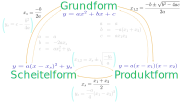
\includegraphics[width=15cm]{allg/funktionen/img/formen/formen.png}
\end{center}

\begin{bemerkung}{}{}
  Das $a$,  ist in allen Formen derselbe Wert und bestimmt die Parabelöffnung.
  \end{bemerkung}
\newpage

\textbf{Grundform aus Scheitelform} (einfaches Ausmultiplizieren). Beispiel:
$$y=2(x-3)^2-4 = 2(x^2-6x+9)-4=2x^2-12x+14$$

\begin{tabular}{rcl}
$a(x-x_S)^2+y_S$ &=& $ax^2-2ax_Sx + (ax_S^2+y_S)$\\
  $a$ &=& $a$ \\
  $b$ &=& $-2ax_S$\\
  $c$ &=& $ax_S^2+y_S$
\end{tabular}


\textbf{Grundform aus Produktform} (einfaches Ausmultiplizieren). Beispiel
$$y=2(x+3)(x-4)=2(x^2 +(3-4)x - 12) = 2x^2-x-24$$

\begin{tabular}{rcl}
  $a(x-x_1)(x-x_2)$ &=& $ax^2 - a(x_1+x_2)x + ax_1x_2$\\
  $a$ &=& $a$ \\
  $b$ &=& $-a(x_1+x_2)$\\
  $c$ &=& $ax_1x_2$
\end{tabular}


\textbf{Nullstellenform (Produktform) aus Grundform}:
Gegeben: $y = ax^2 + bx + c$

Nullstellenform: $y = a(x-x_1)\cdot{}(x-x_2)$ mit

$$x_{1,2} = \frac{-b \pm \sqrt{b^2-4ac}}{2a}$$

\begin{beispiel}{}{}
Gegeben $y = 5x^2 - 5x - 30$. Schreiben Sie dies in der Produktform (=
Nullstellenform):
\platzFuerBerechnungen{3.2}\TRAINER{$y = 5(x-3)(x+2)$\vspace{4.2cm}}
\end{beispiel}
\newpage


\textbf{Scheitelform aus Grundform}:
$$x_S=\frac{-b}{2a}$$

$y_S$ einfach durch Einsetzen von $x_S$ in die Grundform:
$$y_S=c-\frac{b^2}{4a}$$
 
\textbf{Scheitelform aus Produktform}: $x_S$ ist der Mittelwert der beiden
Nullstellen:
$$x_S=\frac{x_1+x_2}{2}$$
Danach $y_S$ einfach durch Einsetzen von $x_S$ in die Produktform:
$$y_S=\frac{-a}{4}(x_1-x_2)^2$$

\textbf{Produktform aus Scheitelform}: Einfachster Weg geht über die Grundform oder abgekürzt:
$$x_{1,2} =x_S \pm \sqrt{\frac{-y_S}{a}}$$


\subsection{Aufgaben}

\TALS{\olatLinkArbeitsblatt{Umrechnen der Formen}{https://olat.bbw.ch/auth/RepositoryEntry/572162090/CourseNode/103176133021102}{1., 2., 3. und 8.}}



\newpage

% Bereits in typ I II und III eingebaut
%\subsection{Parabel aus drei Punkten}
Vorzeigeaufgabe Marthaler Algebra S. 272 Aufg. 3. b) 


\subsection*{Aufgaben}

\AadBMTA{272}{3. a) c)}%% war Marthaler S. 187 Aufg. 676 a) und b)
\GESOAadBMTA{???}{???}

\newpage



%\newpage

%

%%%%%%%%%%%%%%%%%%%%%%%%%%%%%%%%%%%%%%%%%%%%%%%%%%%%%%%%%%%%%%%%
\subsection{Extremwertaufgaben}



\subsubsection{Aus alter Maturprüfung}

\aufgabenFarbe{Gegeben ist die Funktion $f(x) = x\cdot{}(3-\sqrt{x})$,
  $x\in[0;\infty[$.\\
  a) Bestimmen Sie die Nullstellen und das  Extremum der Funktion
  $f$.\\
  b) Im ersten Quadranten, zwischen dem  Graphen und der
  $x$-Achse ist ein  rechtwinkliges Dreieck $ABC$ einbeschrieben.  Der
  rechte Winkel ist in der Ecke $B$.  Punkt $A$ liegt im Ursprung, $B$
  auf der  $x$-Achse und $C$ auf dem Graphen von $f$. Berechnen Sie
  die Koordinaten des  Punktes $C$ so, dass der Flächeninhalt des
  Dreiecks maximal wird.
}%% END aufgabenFarbe

    
\bbwCenterGraphic{8cm}{tals/fct3/img/Maximieren.png}
\TNTeop{
   a) solve$(f(x)=0,x)$ Somit sind die Nullstellen bei 0 und 9\\
     $\text{fmax}(f(x),x)$ liefert $x=4$ ist Maximalstelle (und auch
     Maximalwert ($f(4)=4$)\\
   b) $\text{fmax}(0.5\cdot{}x\cdot{}f(x), x)$ liefert $x = 5.76$ und
   $f(5.76) = 3.456$}%% End TNTeop
\newpage
\subsection*{Aufgaben}
\AadBMTA{311}{49.}
\AadBMTA{321}{17.}

%\newpage

\section{Berührende Graphen}\index{Graphen!berührende}\index{berührende Graphen}

\textbf{Einführungsbeispiel}


Gegeben ist die Parabel $f: y=\frac{1}{4}x^2 -\frac12x +\frac14$ und von einer
Geraden $g$ ist der $y$-Achsenabschnitt $b = -2$ gegeben.

Gesucht ist von der Geraden $g$ die Steigung $a$ so, dass die
Gerade die Parabel tangiert; also genau in einem Punkt berührt.

Wo (in welchem Punkt $B=(x_B|y_B)$) tangiert also die Gerade $g$ die Parabel $f$?

In der folgenden Skizze sind drei mögliche Geraden mit $y$-Achsenabschnitt
$-2$ gezeichnet. Nur eine dieser drei Geraden \textit{tangiert} die Parabel.

\bbwGraph{-4}{4}{-3}{5}{
  \draw[thick,color=blue,variable=\x,domain=-3.5:4] plot ({\x},   {0.25*\x*\x -0.5*\x + 0.25});

  \draw[color=red,variable=\x,domain=-3:5] plot ({\x},{2*\x -2});
  \draw[color=red,variable=\x,domain=-3:5] plot ({\x},{0.5*\x - 2});
  \draw[color=cyan,thick,variable=\x,domain=-3:5] plot ({\x},{1*\x  -2});

  \bbwDot{3, 1}{green}{north}{B}

  %%%\draw[thick,color=blue,variable=\x,domain=-1:5] plot ({\x}, {0.5*\x*\x - 2*\x + 3}); 
  %%\draw[color=red,variable=\x,domain=-1:5] plot ({\x},{0.5*\x + 1});
  %%\draw[color=red,variable=\x,domain=-1:5] plot ({\x},{0.5*\x - 1.5});
  %%\draw[color=cyan,thick,variable=\x,domain=-1:6] plot ({\x},{0.5*\x  -0.125});
  %%\bbwDot{2.5, 1.125}{green}{north}{P}
}
\newpage
\textbf{Lösungsidee}: Der gesuchte Parameter ist $a$, die Steigung der
Geraden.

Nun berechne die Schnittpunkte/den Schnittpunkt mit $$f(x) = g(x).$$

Das $a$ ist gefunden, sobald die Gleichung $f(x)=g(x)$ genau eine
Lösung aufweist; dann also, wenn


\TNT{2}{die Diskriminante dieser Gleichung
verschwindet.}

Den $x$-Wert dieses Berührungspunktes nennen wir $x_B$:


Ansatz:

$$f(x_B) = g(x_B)$$

\TNT{4.4}{
 
\begin{tabular}{rclr}
$\frac14x_s^2-\frac12x_s+\frac14$          & $=$ &  $ax_s-2$ & \\
$\frac14x_s^2+(-\frac12-a)x_s + \frac94$   & $=$ & $0$       & (I)\\
\end{tabular}
\vspace{10mm}
}%% END TNT

Die Diskriminante $D=B^2 - 4AC$ muss gleich 0 sein. 

\TNT{7.2}{
$A = \frac14$, $B = -\frac12-a$ und $C = \frac94$.

  $$D=0=B^2-4AC = (-\frac12-a)^2  - (4\cdot{}A\cdot{}C)$$
  $$0 = (a^2+a+\frac14) - (4\cdot\frac14\cdot{}\frac{+9}4)$$
$$\Longrightarrow 0 = a^2 + a - 2$$
$$\Longrightarrow a_1 = 1 \text{ und  } a_2 = -2$$
\vspace{40mm}
}%% END TNT
\newpage

Für den \textbf{Berührungspunkt} $B=(x_B|y_B)$ müssen wir nun nur doch das gefundene
$a$ in die Gleichung (I) einsetzen.


\TNT{6}{
  $$0 = \frac14x_B^2 + (-\frac12 -a ) + \frac94$$

  $$x_B = x_1 = x_2 = \frac{-B \pm\sqrt{D}}{2A} = \frac{-B \pm
    \sqrt{0}}{2A} = \frac{-B}{2A}$$

  $$x_B = \frac{-B}{2A} = \frac{- (-\frac12 - a)}{\frac24} =
  \frac{\frac12 + a}{\frac12} = (\frac12 + a) : \frac12 = (\frac12+a)
  \cdot{} 2 = 1+2a$$
}



1. Fall: ($a_1=1$):

\TNT{6}{
$B_1: a_1 = 1:$
  $$x_B = 1+2a = 1 + 2\cdot{}(1) = 3$$

Das $y$ finden wir einfach durch Einsetzen von $x$ in den
Funktionsterm der Geradengleichung.

$$y_1 = a_1x_1 - 2 = 1\cdot{}3-2 = 1$$
und somit ist
$$B_1 = (3 | 1)$$
}%% END TNT



2. Fall: ($a_1=-2$):


\TNTeop{
$B_2: a_2 = -2:$
  $$x_B = 1+2a = 1 + 2\cdot{}(-2) = 1-4=-3$$


$$y_2 = a_2x_2+b = -2\cdot{}3-2 = 4$$
und somit ist
$$B_2 = (-3 | 4)$$

}%% END TNT
\newpage




\begin{rezept}{Berührende Graphen}{}

  Bei Berührungsaufgaben mit Parabeln hilft i.\,d.\,R. das folgende
  Vorgehen:

  \begin{enumerate}
  \item Funktionsterme Gleichsetzen: $$f(x) = g(x)$$
  \item In Grundform bringen: $$f(x) - g(x) = 0  \hspace{40mm}
    (I)$$
  \item Diskriminante $D = 0 $ setzen, um den Parameterwert zu
    bestimmen.
  \item Gleichung $(I)$ auflösen mit dem Wissen $D=0$.
    $$x_B=x_1=x_2= \frac{-B}{2A}$$

  \item Gefundenen Parameter in $x_B=\frac{-B}{2A}$ einsetzen, um $x$
    des Berührungspunktes zu bestimmen.
  \item Das $y_B$ des Berührungspunktes ermitteln, indem wir $x_B$ in
    $f$ oder $g$ einsetzen.
    \end{enumerate}
\end{rezept}


\TRAINER{(Je nach Zeit wäre 699. a) noch eine Vorzeigeaufgabe.)}

\subsection{Aufgaben}
\TRAINER{Achtung, dass nicht das Gleichungssystem bereits
  nach dem Gleichsetzen der Graphen aufgestellt wird. Erst nach dem
  Null-Setzen der Diskriminante erhalten wir eine gültige Gleichung
  für das Gleichungssystem.}
%%\TALSAadBMTA{190}{698., 702., 703., 705.}
\TALSAadBMTA{277}{30. a), 36. a), 40. a) c), 42. a), 43. a), 44. a)}
\newpage


\subsection{Grenzwerte und Steigungsfunktion (Optional)}

Wie macht das ein CAS, dass es den tiefsten bzw. den höchsten Punkt
einer Funktion bestimmen kann? Hier ein Erklärungsversuch am Beispiel
der quadratischen Funktion.
Betrachten wir die allgemeine quadratische Funktion $$p: y=ax^2 + bx +
c$$
Mit dem selben $a$ und dem selben $b$ kann ich eine Gerade $s$
definieren, die ich die (Tangenten-)\textbf{Steigungsfunktion}\footnote{Diese
  Steigungsfunktion wird in der Mathematik die
  \textbf{Ableitung}\index{Ableitung} genannt. Genau genommen handelt
  es sich nicht um die Steigung der Parabel, sondern um die Steigung
  einer im Punkt $P=(X_P|f(x_P))$ angelegter Tangente.} nenne:
$$s: y= 2ax+b$$
\newpage


Diese Steigungsfunktion $s$ gibt in jedem Punkt $x$ die Steigung einer
Tangente an die Parabel $p$ an.

\begin{beispiel}{Parabel}{}
  Gegeben ist die Parabel $$p: y=2.5x^2 - 3x + 6.5\text{.}$$

  Wo (für welches $x$) hat diese Parabel
  ihren Tiefpunkt? \TRAINER{Scheitelpunkt:}

  $$x_B =   \LoesungsRaumLen{8cm}{\frac{-b}{2a} = \frac{-(-3)}{2\cdot{}2.5} = 0.6}$$

  Dies ist gleichzeitig die Nullstelle der
  Steigungsfunktion:

  $$s: y= \LoesungsRaumLen{3cm}{2\cdot{}2.5x - 3}$$

  Nullstelle von $s$:

  $$x_0 = \LoesungsRaumLen{7cm}{\frac{3}{2\cdot{}2.5} = 0.6}$$

  Wir können damit aber auch die Steigung in einem ganz anderen Punkt
  \zB für $x=10$ berechnen. Die Parabel $p$ hat an der Stelle $x=10$
  die Tangentensteigung, die durch die Steigungsfunktion im Punkt $10$
  ermittelt wird:

  $$s(10) = \LoesungsRaumLen{40mm}{2\cdot{}10\cdot{2.5} - 3 = 47}$$
  
\end{beispiel}
\newpage

\begin{beispiel}{Gerade gesucht}{}
Gegeben ist die Parabel $$p: y=4x^2 -6x + 3\text{.}$$ Gesucht ist die Gerade
$g: y=ax+b$, sodass die Gerade die Parabel bei $x=7$ berührt.

\begin{enumerate}
\item Die Steigungsfunktion $s$ lautet: $$s:
  y=\LoesungsRaumLen{5cm}{2\cdot{}4x - 6}$$
  
\item Für $x=7$ hat die Steigungsfunktion den Wert \LoesungsRaumLen{1cm}{50}, und somit hat
  die Parabel bei $x=7$ die Steigung \LoesungsRaumLen{1cm}{50}.

  
\item Um den Berührungspunkt $B$ zu finden, setzen wir 7 diesen in $p$
  ein
  $$p(7)= \LoesungsRaumLen{5cm}{4\cdot{}49-6\cdot{}7+3 = 157}$$
  und somit ist
  $$B=(\LoesungsRaum{7}|\LoesungsRaum{157})$$
  
\item Die gesuchte Gerade $g: y=ax+b$ hat also auch die Steigung \LoesungsRaum{50}
  und verläuft durch den Berührungspunkt $B=(\LoesungsRaumLen{9mm}{7}|\LoesungsRaumLen{11mm}{157})$. Also
  $$\LoesungsRaumLen{7cm}{157=50\cdot{}7+b}$$

  Somit ist das gesuchte
  $$b = \LoesungsRaumLen{55mm}{157-50\cdot{}7=-193}$$
  
  und die gesuchte Funktionsgleichung der Geraden lautet: $$y = \LoesungsRaumLen{22mm}{50x-193}$$
  \end{enumerate}
\end{beispiel}

\TRAINER{Idee: Auf mm-Papier eine Funktion $y=\frac1{27}x^3-\frac19
  x^2 - \frac89 x$ vorgeben.

Auftrag: Legen Sie in 5 Punkten eine Tangente an die Funktion und
bestimmen Sie deren Steigung.
Tragen Sie die Steigung in ein neues Koordinatensystem ein: $x$-Achse
= $x$ Wert, $y$-Achse = Steigung der Funktion.
$$f' : y = \frac19 (x-1)^2 - 1 $$
}%%
\newpage

\subsubsection{Beweis der Formel der (Tangenten-)Steigungsfunktion}

Betrachten wir auf auf der $x$-Achse zwei benachbarte Punkte $x$ und
$x+\Delta$. Die Funktionswerte lauten $f(x)$ und $f(x+\Delta)$. Die
\textbf{Steigung} kann nun für eine Gerade bestimmt werden durch:

\bbwCenterGraphic{7cm}{tals/fct3/img/Steigungsfunktion.jpg}

$$\frac{f(x+\Delta) - f(x)}{\Delta}$$

Dies gilt für eine Parabel $p: y=ax^2+bx+c$ näherungsweise auch:
$$\frac{f(x+\Delta)-f(x)}{\Delta} = \frac{(a(x+\Delta)^2 + b(x+\Delta)
  + c) - (ax^2 + bx +c)}{\Delta}=2ax+a\Delta+b$$

Wenn wir nun das $\Delta$ gegen Null gehen lassen, also immer kleinere
Werte einsetzen, so verschwindet der Term $a\cdot{}\Delta$ fast und unsere
Formel stimmt annähernd --- jedoch präzise genug, um dies als Beweis
gelten zu lassen.

Ein anderer Beweis wäre die Tangente effektiv einzusetzen und diese so
zu wählen, dass es genau einen Schnittpunkt gibt, was wieder darauf
zurückführt, dass die Diskriminante = Null gesetzt werden muss. Dann
sind wir exakt, aber der Beweis ist ungleich aufwändiger.
\newpage


\newpage



%% Funktionen II TALS
%%%%%%%%%%%%%%%55
%% Funktionen II TALS Metapackage
\part{Funktionen II}\index{Funktionen!II|textbf}
\renewcommand{\bbwPartID}{FCT2}
%%
%% 2019 07 04 Ph. G. Freimann
%%

\section{Quadratische Funktionen}\index{Funktionen!quadratische}
\sectuntertitel{Geraden im Lande der Parabeln wird dringend angeraten, einen
  Integrationskurs zu besuchen.}
%%%%%%%%%%%%%%%%%%%%%%%%%%%%%%%%%%%%%%%%%%%%%%%%%%%%%%%%%%%%%%%%%%%%%%%%%%%%%%%%%

%%\bbwCenterGraphic{8cm}{tals/fct2/img/lugano2018.jpg}
%%\textit{Bildlegende: Parabeln in Lugano (2018)}
\bbwCenterGraphic{175mm}{tals/fct2/img/paris2022.jpg}
\textit{Bildlegende: Parabeln in den Gärten von Versailles (2022)}

\subsection*{Lernziele}

\begin{itemize}
\item Definition
\item Formen: Scheitel-, Produkt-, Normalform
\item Graphische Darstellung
\item Translationen und Spiegelungen
\end{itemize}

\TadBMTA{260}{15}
%%\TALS{(\cite{frommenwiler17alg} S.183 (Kap. 3.4))}
%%\GESO{(\cite{marthaler21alg}       S.260 (Kap. 15))}

Einstieg: Bilder von Heimgartner/Hunziker.


\textbf{Einstiegsaufgabe: } \aufgabenFarbe{Lösen Sie Aufgaben 1. und 2.
  von Seite 272: Welche der angegebenen Funktionen sind quadratisch?}

\newpage

\subsection{Parabel}\index{Parabel}\index{Normalparabel}

Zeichnen Sie die Funktionen $f: y=x^2$ (= Normalparabel), $y=\frac{1}{3}x^2$

und $y=-0.25\cdot{}x^2$  ins Koordinatensystem:

\bbwGraph{-3}{3}{-3}{7}{
  \TRAINER{\bbwFuncC{\x * \x}{-2.5:2.5}{green}
    \bbwFuncC{-0.25*\x * \x}{-3:3}{green}
    \bbwFuncC{\x * \x / 3}{-3:3}{green}
  }
}


\newpage

\subsection{Grundform}\index{Grundform!quadratische Funktion}\index{Quadratische Funktion!Grundform}
Die Funktion $f(x): x \mapsto y = ax^2 + bx +c$ ist eine
quadratische Funktion in Grundform\index{Grundform!quadratische Funktion}.

Spielen Sie mit \TALS{dem TI-nSpire oder mit} \texttt{geogebra.org} an den Parametern $a$, $b$ und $c$ der Funktionsgleichung $y = a\cdot{}x^2 + b\cdot{} x + c$ herum. Was bewirkt der Parameter

$a$: \LoesungsRaumLang{Parabelöffnung: $|a|$ klein: Breite (weite) Öffnung / $|a|$ groß: Enge, schmale Öffnung. $a < 0$: Parabel ist nach unten geöffnet. $a > 0$: Parabel ist nach oben geöffnet.}

$b$: \LoesungsRaumLang{«Parabelsteigung»\footnote{Mit «Parabelsteigung» ist hier die Steigung der entsprechenden Tangente gemeint.} im Punkt $A(0|c)$}

$c$: \LoesungsRaumLang{$y$-Achsenabschnitt. Damit wird eine Verschiebung der Parabel entlang der $y$-Achse erreicht.}

Versuchen Sie eine Parabel mit Scheitelpunkt $(1|1)$ zu finden\TRAINER{(Lösung: $b=-2a$ und $a+b+c=1$.)}.

\subsection*{Aufgaben}
%%\TALSAadBMTA{184ff}{660. a) c) f), 662. a) b) c) und e)}
\AadBMTA{273}{5., 6., 7., 8. und 9.}
\newpage

\subsection{Vier charakteristische Punkte}
Zeichnen Sie die Funktion
$$p: y = x^2 - 4x + \frac{7}{4}$$

\bbwGraph{-3}{6}{-3}{2}{
\TRAINER{\bbwFunc{\x*\x - 4*\x + 1.75}{-0.2:4}}
}%% end BBW Graph

Wo befinden sich die charakteristischen Punkte?

\TNT{2.4}{\vspace{24mm}}


Die charakteristischen Punkte sind:
\begin{itemize}
\item Schnittpunkt mit $y$-Achse = (\LoesungsRaum{0} | \LoesungsRaum{1.75})
\item Nullstellen: $N_1=(\LoesungsRaum{0.5}| \LoesungsRaum{0}), N_2=( \LoesungsRaum{3.5}|\LoesungsRaum{0})$
\item Scheitelpunkt: $S=(\LoesungsRaum{2}|\LoesungsRaum{-2.25})$
\end{itemize}
 
Wie berechnen sich nun diese Punkte?
\newpage
\subsubsection{Parabelöffnung}
Eigentlich ist die Parabelöffnung kein charakteristischer
Punkt. Dennoch kann man eine $x$-Einheit vom Scheitelpunkt entfernt,
das $a$ der Grundform ($y=ax^2+bx+c$) direkt ablesen. Gehen wir bei
der Normalparabel ($a=1$) vom
Scheitelpunkt um eine Einheit nach rechts, so muss die Parabel um eine
$y$-Einheit nach oben anwachsen.

\TNT{10}{
Parabel durch Scheitelpunkt $P=(-3|1)$ und durch $(-2|2)$ =
verschobene Normalparbel zeichnen.

Parabel mit Scheitelpunkt $P=(2|2)$ durch $(3|0.5)$ zeichnen. Das $a$
ist somit sofort $a=-1.5$ abzulesen.
}

\subsubsection{$y$-Achsenabschnitt}
Genau wie bei der linearen Funktion, gilt für den $y$-Achsenabschnitt,
dass die $x$-Koordinate dieses Punktes Null ist.
$$y = x^2 -4x + 1.75$$
wird mit $x=0$ zu
$y = 1.75$.

Der $y$-Achsenabschnitt ist somit immer das $c$ aus $y = ax^2 + bx +
c$.

\newpage

\subsubsection{Nullstellen}
Wie bei den linearen Funktionen sind auch hier die
Nullstellen die Schnittpunkte mit der $x$-Achse. Dies bedeutet für die
Nullstellen $N(x_0 | y_0)$, dass die $y$-Koordinate = 0 ist. Es gilt
also

$$0 = x^2 - 4 x + \frac{7}{4} $$

Dies ist eine quadratische Gleichung mit den Lösungen:

$$x_{1,2} = \frac{-b \pm \sqrt{b^2-4ac}}{2a}$$ 

\noTRAINER{\platzFuerBerechnungen{2.4}}
\TRAINER{$x_{1} = 0.5; x_{2}=3.5$ (Mitternachtsformel)
  \vspace{3cm}}

\begin{bemerkung}{}{}
  Die Nullstellen der quadratischen Funktion entsprechen den Lösungen
  der zugehörigen quadratischen Funktion (mit $y=0$). Daher gilt
  auch hier: 


  \begin{tabular}{c|p{8cm}}
    Diskriminante $D=b^2-4ac$ > 0 & Es gibt zwei Nullstellen. \\
    \hline\\
    Diskriminante $D=b^2-4ac$ = 0 & Es gibt eine Nullstelle, denn der Scheitelpunkt liegt auf der $x$-Achse.\\
    \hline\\
    Diskriminante $D=b^2-4ac$ < 0 & Es gibt keine Nullstellen, denn die Parabel schneidet die $x$-Achse nicht.\\
  \end{tabular}
  
 \ifisALLINONE{Zum Begriff \textbf{Diskriminante}:  \totalref{diskriminante}}\fi{} 
\end{bemerkung}

\subsection*{Aufgaben}
\AadBMTA{277ff}{28. a) c) }

\newpage



\subsubsection{Scheitelpunkt}\index{Scheitelpunkt}
Der Tief- bzw. Hochpunkt einer Parabel wird \textbf{Scheitelpunkt}
genannt.

Wir berechnen den Scheitelpunkt in zwei Schritten.

\textbf{Erstens:} Wir berechnen den Mittelwert der beiden Nullstellen:
$$x_S := \frac{x_{1} + x_{2}}{2} = \frac{\frac{-b+\sqrt{D}}{2a} + \frac{-b-\sqrt{D}}{2a}}{2} =
\frac{(-b+\sqrt{D}) + (-b-\sqrt{D})}{4a} =\frac{-b}{2a}$$
Dabei ist $D$ die Diskriminante $D=b^2-4ac$.

\platzFuerBerechnungen{2.4}
\TRAINER{$x_S = 2$
\vspace{3cm}}

\textbf{Zweitens:} Wir setzen den gefundenen $x$-Wert
(\LoesungsRaum{2}) in die Funktionsgleichung
ein:
$$y_S = x^2 - 4x + 1.75$$
$$y_S = (\LoesungsRaum{2})^2 - 4\cdot{}(\LoesungsRaum{2}) + 1.75$$

Wir erhalten für den Scheitelpunkt $S$: $S=(x_S | y_S) = (\LoesungsRaum{2} | \LoesungsRaum{-2.25})$.

\begin{gesetz}{Scheitelpunkt}{}
  Der Scheitelpunkt $S$ einer Parabel in der Grundform ($y=ax^2+bx+c$) kann wie folgt
  berechnet werden:

  $$S=\left(\frac{-b}{2a}\middle|\frac{4ac-b^2}{4a}\right)$$

  (Bem.: Der $y$-Wert kann einfach durch Einsetzen des $x$-Wertes in
  die Funktionsgleichnug gefunden werden.)
  \end{gesetz}
  
\subsection*{Aufgaben}
%%\TALSAadBMTA{184ff}{665. a) b) c) 666. a) b) c) e) f) g)}
\AadBMTA{273}{4. (=Aufg. 22. S. 276)}

\newpage

\subsection{Bestimmen der Funktionsgleichung}
\TALS{S. 187 Kap. 3.4.3}

\subsubsection{Referenzaufgaben}

\textbf{TYP I}

Gegeben ist ein Punkt $P$ mit den Koordinaten $(2.3 | -1.5)$. Gesucht ist die reinquadratische Funktion $f: y=a\cdot{}x^2$, welche durch diesen Punkt geht.
Machen Sie vorab eine Skizze.

\bbwGraph{-3}{3}{-2}{1}{
  \TRAINER{\bbwFunc{-0.2836 * \x * \x}{-2.5:2.5}
    \bbwDot{2.3,-1.5}{blue}{west}{P}
  }%% end TRAINER
}%% end BBW Graph

\platzFuerBerechnungen{3.6}

\TRAINER{Idee: Punkt einsetzen: $-1.5 = a\cdot{}(2.3)^2$. Das Auf"|lösen dieser Gleichung liefert $a = \frac{-1.5}{2.3^2}$. Dies liefert $a\approx -0.2836$}

Weitere «TYP 1» Aufgaben wären z. B. $y = 3x^2 - bx + 4$ oder $y=2x^2
-7x + c$ mit anderen Worten alle Parabeln mit genau \textbf{einem}
Parameter, daher «Typ 1».

\newpage



\textbf{TYP II}

Gegeben sind zwei Punkte und wir haben zwei Unbekannte.

\begin{rezept}{}{}
  Gesucht sind $a$ und $c$ aus $y = ax^2 + c$ bei den gegebenen
  Punkten $(7|5)$ und $(2|-4)$.

  Wir lösen dies auch durch Einsetzen der Punkte in die
  Funktionsgleichung und wir erhalten zwei Gleichungen:


  \begin{tabular}{c | r  c  r |}
    (I)  &  $5$ & = & $(7)^2\cdot{} a + c$ \\
    (II) & $-4$ & = &  $(2)^2\cdot{} a + c$ \\
  \end{tabular}

  Durch Subtrahieren der Gleichungen erhalten wir

  \begin{tabular}{c | r  c  r | c}
    (I)  &  $5$ & = & $49\cdot{} a + c$ & \,\\
    (II) & $-4$ & = &  $4\cdot{} a + c$ & $\ominus$\\
  \end{tabular}

  $$9 = 45a$$ und somit
  $$a =\frac{1}{5}.$$

  Dieses $a$ (= $\frac{1}{5}$) setzen wir nun in eine der Gleichungen
  (\zB (I)) ein und erhalten
  $$5=49\cdot{}\frac{1}{5} + c$$
  und nach Auf"|lösen erhalten wir $c=\frac{-24}{5}$.

  Die gesuchte Gleichung lautet also:

  $$y = \frac{1}{5}x^2 - \frac{24}{5}$$
\end{rezept}

Probe durch Einsetzen der $x$-Werte der Punkte in die gefundene Funktionsgleichung:

\TNTeop{}
%%\newpage

\begin{beispiel}{}{}
  Anstelle von $a$ und $c$ können natürlich auch $a$ und $b$ gesucht
  sein. Daher eine zweite Aufgabe.

  Gesucht sind $a$ und $b$ aus $y = ax^2 + bx$ bei den gegebenen

  Punkten $(2|-6)$ und $(-3|5)$.

  Wir lösen dies wiederum durch Einsetzen der Punkte in die
  Funktionsgleichung und wir erhalten die beiden Gleichungen, welche
  wir durch das Additionsverfahren lösen können:

  \begin{tabular}{c | r  c  r | c}
    (I)  &  $-6$ & = & $4a + 2b$ & $\cdot{} 3$ \\
    (II) &   $5$ & = & $9a - 3b$ & $\cdot{} 2$ \\
  \end{tabular}

  somit:
  
  \begin{tabular}{c | r  c  r | c}
    (I')  & $-18$ & = & $12a + 6b$ &\, \\
     \,   & \,    & \,&   \,       & $\oplus$\\
    (II') &  $10$ & = & $18a - 6b$ &\, \\
  \end{tabular}

  Nach Addition der Gleichungen erhalten wir

  $$-8 = 30a$$

  was uns zu $a=\frac{-4}{15}$ bringt.

Dieses $a$ können wir nun wieder in eine der beiden Gleichungen
einsetzen (\zB in (I)):

$$-6=4\cdot{}\frac{-4}{15} + 2b$$

Das Auf"|lösen obiger Gleichung liefert nach Kürzen: $b=\frac{-37}{15}$.

Die gesuchte Funktionsgleichung lautet also

$$y = \frac{-4}{15} x^2 - \frac{37}{15} x.$$

\end{beispiel}

Auch bei «Typ II» kann natürlich jede \textbf{zwei}parametrige quadratische
Funktion herhalten, wie \zB $y=-6cx^2 + bx - c$ durch \textbf{zwei}
gegebene Punkte.
\newpage


\textbf{TYP III}: Gegeben sind hier drei Punkte, wir haben aber auch
drei Unbekannte in $y = ax^2 + bx + c$. Die Punkte sind hier
(1|3), (2|3.5) und (-3|11).

Durch Einsetzen der drei Punkte je in die Funktionsgleichung erhalten
wir drei Gleichungen:

\begin{tabular}{c|r c rcrcr|}
  (I)   & 3   & = & $(1)^2\cdot{}a$  &$+$& $(1)\cdot{}b$  &$+$& c \\ 
  (II)  & 3.5 & = & $(2)^2\cdot{}a$  &$+$& $(2)\cdot{}b$  &$+$& c \\ 
  (III) & 11  & = & $(-3)^2\cdot{}a$ &$+$& $(-3)\cdot{}b$ &$+$& c \\ 
\end{tabular}

Vereinfachen:

\begin{tabular}{c|r c rcrcr|}
  (I)   & 3   & = & $a$  &$+$& $b$  &$+$& c \\ 
  (II)  & 3.5 & = & $4a$ &$+$& $2b$ &$+$& c \\ 
  (III) & 11  & = & $9a$ &$-$& $3b$ &$+$& c \\ 
\end{tabular}

Nun finden wir $a$, indem wir zunächst $c$ durch Subtraktion
eliminieren:

\begin{tabular}{l|r c rcr|}
  (IV) = (II) -   (I) & 0.5  & = & $3a$ &$+$& $b$ \\ 
  (V)  = (III) - (II) & 7.5  & = & $5a$ &$-$& $5b$ \\ 
\end{tabular}

Multiplizieren wir nun die Gleichung (IV) mit 5, so erhalten wir

\begin{tabular}{r|r c rcr|}
  5$\cdot{}$(IV)  & 2.5  & = & $15a$ &$+$& $5b$ \\ 
  (V)             & 7.5  & = & $5a$  &$-$& $5b$ \\ 
\end{tabular}

Durch Addition der beiden Gleichungen (IV) und (V) erhalten wir

$10 = 20a$ oder $a = \frac{1}{2}$.

Um $b$ zu finden, setzen wir $a = \frac{1}{2}$ in (V) ein: $7.5 =
5\cdot{}\frac{1}{2} - 5b$.

Auf"|lösen nach $b$ ergibt $b = -1$.

Zu guter Letzt setzen wir $a = \frac{1}{2}$ und $b=-1$ in die
Gleichung (I) ein, um noch $c$ zu erhalten:

$$3 = a + b + c = \frac{1}{2} - 1 + c$$

Somit ist $c=3.5$ und die Funktionsgleichung lautet:

$$y = \frac{1}{2}x^2 - x + 3.5$$


\TALS{\subsection*{Aufgaben}}
%%\TALSAadBMTA{187ff}{676. a) c), 682., 684.}
\AadBMTA{272}{3. a) c), 20. a) c), 21., 22., 24. a), 25. b)}
\newpage


\subsection{Computer Algebra Systeme (CAS)}\index{CAS}
Das eben gezeigte Beispiel wird in der Praxis meist nicht von Hand,
sondern mit einem Computer-Algebra-System, kurz CAS, gelöst:

\paragraph{Aufgabenstellung}
Gegeben sind wieder drei Punkte (1|3), (2|3.5) und (-3|11).
Gesucht ist die Parabel $y = ax^2 + bx + c$, welche durch die drei
Punkte geht.

Dies wird mit dem \tinspire{} wie folgt gelöst:
\begin{itemize}
\item Definiere die Funktionsgleichung mit
  Parametern\footnote{\tinspire Regel: $ax\ne a\cdot{} x$}:\\
  $$f(x) := a\cdot{}x^2 + b\cdot{}x + c$$
\item Definiere das Gleichungssystem:
  $$gls := \left\{ \begin{array}{l}
    f(1) = 3\\
    f(2) = 3.5\\
    f(-3)= 11\\
  \end{array}\right.$$
\item Löse das Gleichungssystem:
  $$solve(gls,\{a, b, c\})$$
\end{itemize}

\subsection*{Aufgaben}
\AadBMTA{272}{3. b) d)}

\newpage

\subsection{Formen der quadratischen Funktion}
\subsubsection{Nullstellenform}\index{Nullstellenform}

Die \textbf{Nullstellenform} wird auch  «faktorisierte Form» oder
«Produktform» genannt.\index{faktorisierte Form}\index{Produktform}

Beachten Sie die folgende quadr. Funktionsgleichung:

$$y = 3.1(x-5)(x+6)$$

Dies ist eine quadratische Funktion in der sogenannten
\textbf{Nullstellenform}, denn die Nullstellen (hier $x_0 = 5$ oder
$x_0 = -6$) können direkt aus der Funktionsgleichung abgelesen werden.
Wenn wir $y=0$ in die Gleichung setzen (Nullstelle),

$$0 = 3.1(x-5)(x+6)$$
so wird die Gleichung genau dann wahr, wenn (mind.) einer der beiden Klammerausdrücke rechts
gleich Null ist. Die Parabelöffnung (hier 3.1) kann dabei beliebig variieren und ist (neben den Nullstellen) der einzige Parameter.

Die Nullstellenform lautet

\begin{gesetz}{}{}

  $$y = a(x-x_1)\cdot{}(x-x_2)$$

  \end{gesetz}

wobei $x_1$ und $x_2$ die Nullstellen der Parabel bezeichnen. 
\newpage


\subsubsection*{Referenzaufgabe zur Nullstellenform}

\noTRAINER{\bbwGraphic{16cm}{tals/fct2/img/BrunnenNullstellenformOhneKoordinatensystem.png}}
\TRAINER{\bbwGraphic{16cm}{tals/fct2/img/BrunnenNullstellenformMitKoordinatensystem.png}}

Ein parabelförmiger Wasserstrahl spritzt ebenerdig aus einem Brunnen und trifft 7m von der Düse entfernt wieder auf dem Boden auf.
Das Wasser steigt also erst gleich hoch an, wie es danach wieder «herunterfällt».
Dabei wird gemessen, dass 1m von der Düse entfernt der Wasserstrahl 84cm über Boden verläuft.
Können Sie aufrecht unter dem Wasserstrahl hindurchgehen?

Tipp: Skizze und  die Parabelgleichung in Nullstellenform aufschreiben. Die Düse ist der Ursprung der Koordinatensystems.\\

\TNT{5.2}{Die Funktionsgleichung lautet $y=a(x-x_1)(x-x2)$.\\
  Mit den Nullstellen $x_1=0$ und $x_2=7$.\\
  Wir setzen den gemessenen Punkt (1|0.84) in die Gleichung ein und erhalten $0.84 = a\cdot{}(1-0)(1-7)$.\\
  Daraus ergibt sich $a=0.84/(-6) = -0.14 $.\\
  Nun setzen wir 3.5 Meter in die Funktionsgleichung $y = -0.14(x-0)(x-7)$ ein: und erhalten $y=-01.4\cdot{}3.5\cdot{}(-3.5) = 1.715m$; das ist die höchste Parabelstelle.}


\subsection*{Aufgaben}%% Nullstellenform
%%\TALSAadBMTA{185}{663, 678., 680.}
\TALSAadBMTA{277}{30. a) b), 31. b)}
\newpage

%%\TRAINER{\, \newpage}
\subsubsection{Scheitelform}\index{Scheitelform!der quadratischen
  Funktion}
Einstieg: Wo hat die Parabel $f: y=3.6(x-4)^2 + 5$ ihren
Scheitelpunkt?

\TNT{4.4}{CAS: bei $x_S = 4$ und $y_S= 5$; völlig irrelevant ist die 3.6.}

Ist eine quadratische Funktion in der Form
\begin{gesetz}{}{}
$$y = a(x-x_S)^2 + y_S$$
\end{gesetz}
gegeben, so sprechen wir von der \textbf{Scheitelform} oder Scheitelpunktsform.
Das liegt daran, dass diese Parabel ihren Scheitelpunkt bei
$(x_S|y_S)$ hat.

Setzen wir für $x$ = $x_S$ in die Funktionsgleichung, so erhalten wir
gerade die $y$-Koordinate des Scheitelpunktes. Je weiter wir uns nun
mit $x$ von $x_S$ wegbewegen, umso größer wird der Term $(x-x_S)^2$
und zwar in egal welcher Richtung wir uns von $x_S$ wegbewegen, die
$y$-Koordinate verhält sich in beiden Fällen symmetrisch.

Prüfen Sie dies mit TI-nSpire oder \texttt{geogebra.org} an der Funktion

$$y = a\cdot{}(x-p)^2 + q$$

Definieren Sie dabei auch den Punkt $S=(p|q)$. Spielen Sie nun mit
$a$, $p$ und $q$. Was bewirken die Änderungen?
\newpage


\subsubsection{Referenzaufgabe Scheitelform}
Von einer Parabel ist der Scheitel $S(2|3)$ gegeben. Ebenfalls ist bekannt, dass die Parabel durch den Punkt $P\left(-\frac{1}{2}\middle|1\right)$ geht.

  Berechnen Sie die Funktionsgleichung in der Grundform $y = ax^2 + bx + c$. Tipp:
  Schreiben Sie die Funktionsgleichung in der Form $y=a(x - x_S)^2 +  y_S$ und setzen anschließend den Punkt $P$ ein.

  \platzFuerBerechnungen{8.0}%%
  \TRAINER{
    Ansatz:
    $$y = a(x-2)^2 + 3$$
    Jetzt $P$ einsetzen:
    $$1 = a(-\frac{1}{2} - 2)^2 + 3 $$
    Nach $a$ auf"|lösen ergibt:
    $$a=-0.32 (=\frac{-2}{2.5^2})$$
    Nun setzen wir $a=-0.32$ in die Funktionsgleichung $y=a(x-2)^2+3$
    ein:
    $$y=-0.32(x-2)^2+3$$
    und quadrieren das Binom, um die geforderte Grundform zu erhalten:
    $$y = -0.32(x^2 - 4x + 4) + 3 = -0.32x^2 + 1.28x + 1.72$$
  }%%end TRAINER%%

  \subsection*{Aufgabe}
  \AadBMTA{277}{29. a) c) e), 32. a), 33.}
%%  \TALSAadBMTA{185}{679. a), 681., 695., 684. a), 700., 694., 686.(*) und  664.}}

\newpage


\subsection{Umrechnungen der Formen}\index{Formen!der quadratischen Funktion}\index{Quadratische Funktion!Formen}

Nochmals die drei Formen im Überblick:


\begin{tabular}{c|l}
  Form & Funktionsgleichung\\
  \hline\\
  Normalform/Grundform & $f: y= ax^2 + bx + c$\\
  \hline\\
  Nullstellenform, faktorisierte Form oder Produktform & $f: y=a(x-x_0)(x-x_1)$\\
  \hline\\
  Scheitelform & $f: y=a(x-x_S)^2+y_S$\\
  \hline%%
\end{tabular}


\subsubsection{Umrechnungen zwischen den Formen}\index{Umrechnungen!quadratische Funktion}\index{Quadratische Funktion!Umrechnungen}

\begin{center}
  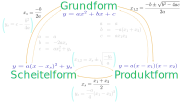
\includegraphics[width=15cm]{allg/funktionen/img/formen/formen.png}
\end{center}

\begin{bemerkung}{}{}
  Das $a$,  ist in allen Formen derselbe Wert und bestimmt die Parabelöffnung.
  \end{bemerkung}
\newpage

\textbf{Grundform aus Scheitelform} (einfaches Ausmultiplizieren). Beispiel:
$$y=2(x-3)^2-4 = 2(x^2-6x+9)-4=2x^2-12x+14$$

\begin{tabular}{rcl}
$a(x-x_S)^2+y_S$ &=& $ax^2-2ax_Sx + (ax_S^2+y_S)$\\
  $a$ &=& $a$ \\
  $b$ &=& $-2ax_S$\\
  $c$ &=& $ax_S^2+y_S$
\end{tabular}


\textbf{Grundform aus Produktform} (einfaches Ausmultiplizieren). Beispiel
$$y=2(x+3)(x-4)=2(x^2 +(3-4)x - 12) = 2x^2-x-24$$

\begin{tabular}{rcl}
  $a(x-x_1)(x-x_2)$ &=& $ax^2 - a(x_1+x_2)x + ax_1x_2$\\
  $a$ &=& $a$ \\
  $b$ &=& $-a(x_1+x_2)$\\
  $c$ &=& $ax_1x_2$
\end{tabular}


\textbf{Nullstellenform (Produktform) aus Grundform}:
Gegeben: $y = ax^2 + bx + c$

Nullstellenform: $y = a(x-x_1)\cdot{}(x-x_2)$ mit

$$x_{1,2} = \frac{-b \pm \sqrt{b^2-4ac}}{2a}$$

\begin{beispiel}{}{}
Gegeben $y = 5x^2 - 5x - 30$. Schreiben Sie dies in der Produktform (=
Nullstellenform):
\platzFuerBerechnungen{3.2}\TRAINER{$y = 5(x-3)(x+2)$\vspace{4.2cm}}
\end{beispiel}
\newpage


\textbf{Scheitelform aus Grundform}:
$$x_S=\frac{-b}{2a}$$

$y_S$ einfach durch Einsetzen von $x_S$ in die Grundform:
$$y_S=c-\frac{b^2}{4a}$$
 
\textbf{Scheitelform aus Produktform}: $x_S$ ist der Mittelwert der beiden
Nullstellen:
$$x_S=\frac{x_1+x_2}{2}$$
Danach $y_S$ einfach durch Einsetzen von $x_S$ in die Produktform:
$$y_S=\frac{-a}{4}(x_1-x_2)^2$$

\textbf{Produktform aus Scheitelform}: Einfachster Weg geht über die Grundform oder abgekürzt:
$$x_{1,2} =x_S \pm \sqrt{\frac{-y_S}{a}}$$


\subsection{Aufgaben}

\TALS{\olatLinkArbeitsblatt{Umrechnen der Formen}{https://olat.bbw.ch/auth/RepositoryEntry/572162090/CourseNode/103176133021102}{1., 2., 3. und 8.}}



\newpage

% Bereits in typ I II und III eingebaut
%\subsection{Parabel aus drei Punkten}
Vorzeigeaufgabe Marthaler Algebra S. 272 Aufg. 3. b) 


\subsection*{Aufgaben}

\AadBMTA{272}{3. a) c)}%% war Marthaler S. 187 Aufg. 676 a) und b)
\GESOAadBMTA{???}{???}

\newpage



%\newpage

%

%%%%%%%%%%%%%%%%%%%%%%%%%%%%%%%%%%%%%%%%%%%%%%%%%%%%%%%%%%%%%%%%
\subsection{Extremwertaufgaben}



\subsubsection{Aus alter Maturprüfung}

\aufgabenFarbe{Gegeben ist die Funktion $f(x) = x\cdot{}(3-\sqrt{x})$,
  $x\in[0;\infty[$.\\
  a) Bestimmen Sie die Nullstellen und das  Extremum der Funktion
  $f$.\\
  b) Im ersten Quadranten, zwischen dem  Graphen und der
  $x$-Achse ist ein  rechtwinkliges Dreieck $ABC$ einbeschrieben.  Der
  rechte Winkel ist in der Ecke $B$.  Punkt $A$ liegt im Ursprung, $B$
  auf der  $x$-Achse und $C$ auf dem Graphen von $f$. Berechnen Sie
  die Koordinaten des  Punktes $C$ so, dass der Flächeninhalt des
  Dreiecks maximal wird.
}%% END aufgabenFarbe

    
\bbwCenterGraphic{8cm}{tals/fct3/img/Maximieren.png}
\TNTeop{
   a) solve$(f(x)=0,x)$ Somit sind die Nullstellen bei 0 und 9\\
     $\text{fmax}(f(x),x)$ liefert $x=4$ ist Maximalstelle (und auch
     Maximalwert ($f(4)=4$)\\
   b) $\text{fmax}(0.5\cdot{}x\cdot{}f(x), x)$ liefert $x = 5.76$ und
   $f(5.76) = 3.456$}%% End TNTeop
\newpage
\subsection*{Aufgaben}
\AadBMTA{311}{49.}
\AadBMTA{321}{17.}

%\newpage

\section{Berührende Graphen}\index{Graphen!berührende}\index{berührende Graphen}

\textbf{Einführungsbeispiel}


Gegeben ist die Parabel $f: y=\frac{1}{4}x^2 -\frac12x +\frac14$ und von einer
Geraden $g$ ist der $y$-Achsenabschnitt $b = -2$ gegeben.

Gesucht ist von der Geraden $g$ die Steigung $a$ so, dass die
Gerade die Parabel tangiert; also genau in einem Punkt berührt.

Wo (in welchem Punkt $B=(x_B|y_B)$) tangiert also die Gerade $g$ die Parabel $f$?

In der folgenden Skizze sind drei mögliche Geraden mit $y$-Achsenabschnitt
$-2$ gezeichnet. Nur eine dieser drei Geraden \textit{tangiert} die Parabel.

\bbwGraph{-4}{4}{-3}{5}{
  \draw[thick,color=blue,variable=\x,domain=-3.5:4] plot ({\x},   {0.25*\x*\x -0.5*\x + 0.25});

  \draw[color=red,variable=\x,domain=-3:5] plot ({\x},{2*\x -2});
  \draw[color=red,variable=\x,domain=-3:5] plot ({\x},{0.5*\x - 2});
  \draw[color=cyan,thick,variable=\x,domain=-3:5] plot ({\x},{1*\x  -2});

  \bbwDot{3, 1}{green}{north}{B}

  %%%\draw[thick,color=blue,variable=\x,domain=-1:5] plot ({\x}, {0.5*\x*\x - 2*\x + 3}); 
  %%\draw[color=red,variable=\x,domain=-1:5] plot ({\x},{0.5*\x + 1});
  %%\draw[color=red,variable=\x,domain=-1:5] plot ({\x},{0.5*\x - 1.5});
  %%\draw[color=cyan,thick,variable=\x,domain=-1:6] plot ({\x},{0.5*\x  -0.125});
  %%\bbwDot{2.5, 1.125}{green}{north}{P}
}
\newpage
\textbf{Lösungsidee}: Der gesuchte Parameter ist $a$, die Steigung der
Geraden.

Nun berechne die Schnittpunkte/den Schnittpunkt mit $$f(x) = g(x).$$

Das $a$ ist gefunden, sobald die Gleichung $f(x)=g(x)$ genau eine
Lösung aufweist; dann also, wenn


\TNT{2}{die Diskriminante dieser Gleichung
verschwindet.}

Den $x$-Wert dieses Berührungspunktes nennen wir $x_B$:


Ansatz:

$$f(x_B) = g(x_B)$$

\TNT{4.4}{
 
\begin{tabular}{rclr}
$\frac14x_s^2-\frac12x_s+\frac14$          & $=$ &  $ax_s-2$ & \\
$\frac14x_s^2+(-\frac12-a)x_s + \frac94$   & $=$ & $0$       & (I)\\
\end{tabular}
\vspace{10mm}
}%% END TNT

Die Diskriminante $D=B^2 - 4AC$ muss gleich 0 sein. 

\TNT{7.2}{
$A = \frac14$, $B = -\frac12-a$ und $C = \frac94$.

  $$D=0=B^2-4AC = (-\frac12-a)^2  - (4\cdot{}A\cdot{}C)$$
  $$0 = (a^2+a+\frac14) - (4\cdot\frac14\cdot{}\frac{+9}4)$$
$$\Longrightarrow 0 = a^2 + a - 2$$
$$\Longrightarrow a_1 = 1 \text{ und  } a_2 = -2$$
\vspace{40mm}
}%% END TNT
\newpage

Für den \textbf{Berührungspunkt} $B=(x_B|y_B)$ müssen wir nun nur doch das gefundene
$a$ in die Gleichung (I) einsetzen.


\TNT{6}{
  $$0 = \frac14x_B^2 + (-\frac12 -a ) + \frac94$$

  $$x_B = x_1 = x_2 = \frac{-B \pm\sqrt{D}}{2A} = \frac{-B \pm
    \sqrt{0}}{2A} = \frac{-B}{2A}$$

  $$x_B = \frac{-B}{2A} = \frac{- (-\frac12 - a)}{\frac24} =
  \frac{\frac12 + a}{\frac12} = (\frac12 + a) : \frac12 = (\frac12+a)
  \cdot{} 2 = 1+2a$$
}



1. Fall: ($a_1=1$):

\TNT{6}{
$B_1: a_1 = 1:$
  $$x_B = 1+2a = 1 + 2\cdot{}(1) = 3$$

Das $y$ finden wir einfach durch Einsetzen von $x$ in den
Funktionsterm der Geradengleichung.

$$y_1 = a_1x_1 - 2 = 1\cdot{}3-2 = 1$$
und somit ist
$$B_1 = (3 | 1)$$
}%% END TNT



2. Fall: ($a_1=-2$):


\TNTeop{
$B_2: a_2 = -2:$
  $$x_B = 1+2a = 1 + 2\cdot{}(-2) = 1-4=-3$$


$$y_2 = a_2x_2+b = -2\cdot{}3-2 = 4$$
und somit ist
$$B_2 = (-3 | 4)$$

}%% END TNT
\newpage




\begin{rezept}{Berührende Graphen}{}

  Bei Berührungsaufgaben mit Parabeln hilft i.\,d.\,R. das folgende
  Vorgehen:

  \begin{enumerate}
  \item Funktionsterme Gleichsetzen: $$f(x) = g(x)$$
  \item In Grundform bringen: $$f(x) - g(x) = 0  \hspace{40mm}
    (I)$$
  \item Diskriminante $D = 0 $ setzen, um den Parameterwert zu
    bestimmen.
  \item Gleichung $(I)$ auflösen mit dem Wissen $D=0$.
    $$x_B=x_1=x_2= \frac{-B}{2A}$$

  \item Gefundenen Parameter in $x_B=\frac{-B}{2A}$ einsetzen, um $x$
    des Berührungspunktes zu bestimmen.
  \item Das $y_B$ des Berührungspunktes ermitteln, indem wir $x_B$ in
    $f$ oder $g$ einsetzen.
    \end{enumerate}
\end{rezept}


\TRAINER{(Je nach Zeit wäre 699. a) noch eine Vorzeigeaufgabe.)}

\subsection{Aufgaben}
\TRAINER{Achtung, dass nicht das Gleichungssystem bereits
  nach dem Gleichsetzen der Graphen aufgestellt wird. Erst nach dem
  Null-Setzen der Diskriminante erhalten wir eine gültige Gleichung
  für das Gleichungssystem.}
%%\TALSAadBMTA{190}{698., 702., 703., 705.}
\TALSAadBMTA{277}{30. a), 36. a), 40. a) c), 42. a), 43. a), 44. a)}
\newpage


\subsection{Grenzwerte und Steigungsfunktion (Optional)}

Wie macht das ein CAS, dass es den tiefsten bzw. den höchsten Punkt
einer Funktion bestimmen kann? Hier ein Erklärungsversuch am Beispiel
der quadratischen Funktion.
Betrachten wir die allgemeine quadratische Funktion $$p: y=ax^2 + bx +
c$$
Mit dem selben $a$ und dem selben $b$ kann ich eine Gerade $s$
definieren, die ich die (Tangenten-)\textbf{Steigungsfunktion}\footnote{Diese
  Steigungsfunktion wird in der Mathematik die
  \textbf{Ableitung}\index{Ableitung} genannt. Genau genommen handelt
  es sich nicht um die Steigung der Parabel, sondern um die Steigung
  einer im Punkt $P=(X_P|f(x_P))$ angelegter Tangente.} nenne:
$$s: y= 2ax+b$$
\newpage


Diese Steigungsfunktion $s$ gibt in jedem Punkt $x$ die Steigung einer
Tangente an die Parabel $p$ an.

\begin{beispiel}{Parabel}{}
  Gegeben ist die Parabel $$p: y=2.5x^2 - 3x + 6.5\text{.}$$

  Wo (für welches $x$) hat diese Parabel
  ihren Tiefpunkt? \TRAINER{Scheitelpunkt:}

  $$x_B =   \LoesungsRaumLen{8cm}{\frac{-b}{2a} = \frac{-(-3)}{2\cdot{}2.5} = 0.6}$$

  Dies ist gleichzeitig die Nullstelle der
  Steigungsfunktion:

  $$s: y= \LoesungsRaumLen{3cm}{2\cdot{}2.5x - 3}$$

  Nullstelle von $s$:

  $$x_0 = \LoesungsRaumLen{7cm}{\frac{3}{2\cdot{}2.5} = 0.6}$$

  Wir können damit aber auch die Steigung in einem ganz anderen Punkt
  \zB für $x=10$ berechnen. Die Parabel $p$ hat an der Stelle $x=10$
  die Tangentensteigung, die durch die Steigungsfunktion im Punkt $10$
  ermittelt wird:

  $$s(10) = \LoesungsRaumLen{40mm}{2\cdot{}10\cdot{2.5} - 3 = 47}$$
  
\end{beispiel}
\newpage

\begin{beispiel}{Gerade gesucht}{}
Gegeben ist die Parabel $$p: y=4x^2 -6x + 3\text{.}$$ Gesucht ist die Gerade
$g: y=ax+b$, sodass die Gerade die Parabel bei $x=7$ berührt.

\begin{enumerate}
\item Die Steigungsfunktion $s$ lautet: $$s:
  y=\LoesungsRaumLen{5cm}{2\cdot{}4x - 6}$$
  
\item Für $x=7$ hat die Steigungsfunktion den Wert \LoesungsRaumLen{1cm}{50}, und somit hat
  die Parabel bei $x=7$ die Steigung \LoesungsRaumLen{1cm}{50}.

  
\item Um den Berührungspunkt $B$ zu finden, setzen wir 7 diesen in $p$
  ein
  $$p(7)= \LoesungsRaumLen{5cm}{4\cdot{}49-6\cdot{}7+3 = 157}$$
  und somit ist
  $$B=(\LoesungsRaum{7}|\LoesungsRaum{157})$$
  
\item Die gesuchte Gerade $g: y=ax+b$ hat also auch die Steigung \LoesungsRaum{50}
  und verläuft durch den Berührungspunkt $B=(\LoesungsRaumLen{9mm}{7}|\LoesungsRaumLen{11mm}{157})$. Also
  $$\LoesungsRaumLen{7cm}{157=50\cdot{}7+b}$$

  Somit ist das gesuchte
  $$b = \LoesungsRaumLen{55mm}{157-50\cdot{}7=-193}$$
  
  und die gesuchte Funktionsgleichung der Geraden lautet: $$y = \LoesungsRaumLen{22mm}{50x-193}$$
  \end{enumerate}
\end{beispiel}

\TRAINER{Idee: Auf mm-Papier eine Funktion $y=\frac1{27}x^3-\frac19
  x^2 - \frac89 x$ vorgeben.

Auftrag: Legen Sie in 5 Punkten eine Tangente an die Funktion und
bestimmen Sie deren Steigung.
Tragen Sie die Steigung in ein neues Koordinatensystem ein: $x$-Achse
= $x$ Wert, $y$-Achse = Steigung der Funktion.
$$f' : y = \frac19 (x-1)^2 - 1 $$
}%%
\newpage

\subsubsection{Beweis der Formel der (Tangenten-)Steigungsfunktion}

Betrachten wir auf auf der $x$-Achse zwei benachbarte Punkte $x$ und
$x+\Delta$. Die Funktionswerte lauten $f(x)$ und $f(x+\Delta)$. Die
\textbf{Steigung} kann nun für eine Gerade bestimmt werden durch:

\bbwCenterGraphic{7cm}{tals/fct3/img/Steigungsfunktion.jpg}

$$\frac{f(x+\Delta) - f(x)}{\Delta}$$

Dies gilt für eine Parabel $p: y=ax^2+bx+c$ näherungsweise auch:
$$\frac{f(x+\Delta)-f(x)}{\Delta} = \frac{(a(x+\Delta)^2 + b(x+\Delta)
  + c) - (ax^2 + bx +c)}{\Delta}=2ax+a\Delta+b$$

Wenn wir nun das $\Delta$ gegen Null gehen lassen, also immer kleinere
Werte einsetzen, so verschwindet der Term $a\cdot{}\Delta$ fast und unsere
Formel stimmt annähernd --- jedoch präzise genug, um dies als Beweis
gelten zu lassen.

Ein anderer Beweis wäre die Tangente effektiv einzusetzen und diese so
zu wählen, dass es genau einen Schnittpunkt gibt, was wieder darauf
zurückführt, dass die Diskriminante = Null gesetzt werden muss. Dann
sind wir exakt, aber der Beweis ist ungleich aufwändiger.
\newpage


\newpage



%% Trigonometrie III
%%%%%%%%%%%%%%%55
%% Funktionen II TALS Metapackage
\part{Funktionen II}\index{Funktionen!II|textbf}
\renewcommand{\bbwPartID}{FCT2}
%%
%% 2019 07 04 Ph. G. Freimann
%%

\section{Quadratische Funktionen}\index{Funktionen!quadratische}
\sectuntertitel{Geraden im Lande der Parabeln wird dringend angeraten, einen
  Integrationskurs zu besuchen.}
%%%%%%%%%%%%%%%%%%%%%%%%%%%%%%%%%%%%%%%%%%%%%%%%%%%%%%%%%%%%%%%%%%%%%%%%%%%%%%%%%

%%\bbwCenterGraphic{8cm}{tals/fct2/img/lugano2018.jpg}
%%\textit{Bildlegende: Parabeln in Lugano (2018)}
\bbwCenterGraphic{175mm}{tals/fct2/img/paris2022.jpg}
\textit{Bildlegende: Parabeln in den Gärten von Versailles (2022)}

\subsection*{Lernziele}

\begin{itemize}
\item Definition
\item Formen: Scheitel-, Produkt-, Normalform
\item Graphische Darstellung
\item Translationen und Spiegelungen
\end{itemize}

\TadBMTA{260}{15}
%%\TALS{(\cite{frommenwiler17alg} S.183 (Kap. 3.4))}
%%\GESO{(\cite{marthaler21alg}       S.260 (Kap. 15))}

Einstieg: Bilder von Heimgartner/Hunziker.


\textbf{Einstiegsaufgabe: } \aufgabenFarbe{Lösen Sie Aufgaben 1. und 2.
  von Seite 272: Welche der angegebenen Funktionen sind quadratisch?}

\newpage

\subsection{Parabel}\index{Parabel}\index{Normalparabel}

Zeichnen Sie die Funktionen $f: y=x^2$ (= Normalparabel), $y=\frac{1}{3}x^2$

und $y=-0.25\cdot{}x^2$  ins Koordinatensystem:

\bbwGraph{-3}{3}{-3}{7}{
  \TRAINER{\bbwFuncC{\x * \x}{-2.5:2.5}{green}
    \bbwFuncC{-0.25*\x * \x}{-3:3}{green}
    \bbwFuncC{\x * \x / 3}{-3:3}{green}
  }
}


\newpage

\subsection{Grundform}\index{Grundform!quadratische Funktion}\index{Quadratische Funktion!Grundform}
Die Funktion $f(x): x \mapsto y = ax^2 + bx +c$ ist eine
quadratische Funktion in Grundform\index{Grundform!quadratische Funktion}.

Spielen Sie mit \TALS{dem TI-nSpire oder mit} \texttt{geogebra.org} an den Parametern $a$, $b$ und $c$ der Funktionsgleichung $y = a\cdot{}x^2 + b\cdot{} x + c$ herum. Was bewirkt der Parameter

$a$: \LoesungsRaumLang{Parabelöffnung: $|a|$ klein: Breite (weite) Öffnung / $|a|$ groß: Enge, schmale Öffnung. $a < 0$: Parabel ist nach unten geöffnet. $a > 0$: Parabel ist nach oben geöffnet.}

$b$: \LoesungsRaumLang{«Parabelsteigung»\footnote{Mit «Parabelsteigung» ist hier die Steigung der entsprechenden Tangente gemeint.} im Punkt $A(0|c)$}

$c$: \LoesungsRaumLang{$y$-Achsenabschnitt. Damit wird eine Verschiebung der Parabel entlang der $y$-Achse erreicht.}

Versuchen Sie eine Parabel mit Scheitelpunkt $(1|1)$ zu finden\TRAINER{(Lösung: $b=-2a$ und $a+b+c=1$.)}.

\subsection*{Aufgaben}
%%\TALSAadBMTA{184ff}{660. a) c) f), 662. a) b) c) und e)}
\AadBMTA{273}{5., 6., 7., 8. und 9.}
\newpage

\subsection{Vier charakteristische Punkte}
Zeichnen Sie die Funktion
$$p: y = x^2 - 4x + \frac{7}{4}$$

\bbwGraph{-3}{6}{-3}{2}{
\TRAINER{\bbwFunc{\x*\x - 4*\x + 1.75}{-0.2:4}}
}%% end BBW Graph

Wo befinden sich die charakteristischen Punkte?

\TNT{2.4}{\vspace{24mm}}


Die charakteristischen Punkte sind:
\begin{itemize}
\item Schnittpunkt mit $y$-Achse = (\LoesungsRaum{0} | \LoesungsRaum{1.75})
\item Nullstellen: $N_1=(\LoesungsRaum{0.5}| \LoesungsRaum{0}), N_2=( \LoesungsRaum{3.5}|\LoesungsRaum{0})$
\item Scheitelpunkt: $S=(\LoesungsRaum{2}|\LoesungsRaum{-2.25})$
\end{itemize}
 
Wie berechnen sich nun diese Punkte?
\newpage
\subsubsection{Parabelöffnung}
Eigentlich ist die Parabelöffnung kein charakteristischer
Punkt. Dennoch kann man eine $x$-Einheit vom Scheitelpunkt entfernt,
das $a$ der Grundform ($y=ax^2+bx+c$) direkt ablesen. Gehen wir bei
der Normalparabel ($a=1$) vom
Scheitelpunkt um eine Einheit nach rechts, so muss die Parabel um eine
$y$-Einheit nach oben anwachsen.

\TNT{10}{
Parabel durch Scheitelpunkt $P=(-3|1)$ und durch $(-2|2)$ =
verschobene Normalparbel zeichnen.

Parabel mit Scheitelpunkt $P=(2|2)$ durch $(3|0.5)$ zeichnen. Das $a$
ist somit sofort $a=-1.5$ abzulesen.
}

\subsubsection{$y$-Achsenabschnitt}
Genau wie bei der linearen Funktion, gilt für den $y$-Achsenabschnitt,
dass die $x$-Koordinate dieses Punktes Null ist.
$$y = x^2 -4x + 1.75$$
wird mit $x=0$ zu
$y = 1.75$.

Der $y$-Achsenabschnitt ist somit immer das $c$ aus $y = ax^2 + bx +
c$.

\newpage

\subsubsection{Nullstellen}
Wie bei den linearen Funktionen sind auch hier die
Nullstellen die Schnittpunkte mit der $x$-Achse. Dies bedeutet für die
Nullstellen $N(x_0 | y_0)$, dass die $y$-Koordinate = 0 ist. Es gilt
also

$$0 = x^2 - 4 x + \frac{7}{4} $$

Dies ist eine quadratische Gleichung mit den Lösungen:

$$x_{1,2} = \frac{-b \pm \sqrt{b^2-4ac}}{2a}$$ 

\noTRAINER{\platzFuerBerechnungen{2.4}}
\TRAINER{$x_{1} = 0.5; x_{2}=3.5$ (Mitternachtsformel)
  \vspace{3cm}}

\begin{bemerkung}{}{}
  Die Nullstellen der quadratischen Funktion entsprechen den Lösungen
  der zugehörigen quadratischen Funktion (mit $y=0$). Daher gilt
  auch hier: 


  \begin{tabular}{c|p{8cm}}
    Diskriminante $D=b^2-4ac$ > 0 & Es gibt zwei Nullstellen. \\
    \hline\\
    Diskriminante $D=b^2-4ac$ = 0 & Es gibt eine Nullstelle, denn der Scheitelpunkt liegt auf der $x$-Achse.\\
    \hline\\
    Diskriminante $D=b^2-4ac$ < 0 & Es gibt keine Nullstellen, denn die Parabel schneidet die $x$-Achse nicht.\\
  \end{tabular}
  
 \ifisALLINONE{Zum Begriff \textbf{Diskriminante}:  \totalref{diskriminante}}\fi{} 
\end{bemerkung}

\subsection*{Aufgaben}
\AadBMTA{277ff}{28. a) c) }

\newpage



\subsubsection{Scheitelpunkt}\index{Scheitelpunkt}
Der Tief- bzw. Hochpunkt einer Parabel wird \textbf{Scheitelpunkt}
genannt.

Wir berechnen den Scheitelpunkt in zwei Schritten.

\textbf{Erstens:} Wir berechnen den Mittelwert der beiden Nullstellen:
$$x_S := \frac{x_{1} + x_{2}}{2} = \frac{\frac{-b+\sqrt{D}}{2a} + \frac{-b-\sqrt{D}}{2a}}{2} =
\frac{(-b+\sqrt{D}) + (-b-\sqrt{D})}{4a} =\frac{-b}{2a}$$
Dabei ist $D$ die Diskriminante $D=b^2-4ac$.

\platzFuerBerechnungen{2.4}
\TRAINER{$x_S = 2$
\vspace{3cm}}

\textbf{Zweitens:} Wir setzen den gefundenen $x$-Wert
(\LoesungsRaum{2}) in die Funktionsgleichung
ein:
$$y_S = x^2 - 4x + 1.75$$
$$y_S = (\LoesungsRaum{2})^2 - 4\cdot{}(\LoesungsRaum{2}) + 1.75$$

Wir erhalten für den Scheitelpunkt $S$: $S=(x_S | y_S) = (\LoesungsRaum{2} | \LoesungsRaum{-2.25})$.

\begin{gesetz}{Scheitelpunkt}{}
  Der Scheitelpunkt $S$ einer Parabel in der Grundform ($y=ax^2+bx+c$) kann wie folgt
  berechnet werden:

  $$S=\left(\frac{-b}{2a}\middle|\frac{4ac-b^2}{4a}\right)$$

  (Bem.: Der $y$-Wert kann einfach durch Einsetzen des $x$-Wertes in
  die Funktionsgleichnug gefunden werden.)
  \end{gesetz}
  
\subsection*{Aufgaben}
%%\TALSAadBMTA{184ff}{665. a) b) c) 666. a) b) c) e) f) g)}
\AadBMTA{273}{4. (=Aufg. 22. S. 276)}

\newpage

\subsection{Bestimmen der Funktionsgleichung}
\TALS{S. 187 Kap. 3.4.3}

\subsubsection{Referenzaufgaben}

\textbf{TYP I}

Gegeben ist ein Punkt $P$ mit den Koordinaten $(2.3 | -1.5)$. Gesucht ist die reinquadratische Funktion $f: y=a\cdot{}x^2$, welche durch diesen Punkt geht.
Machen Sie vorab eine Skizze.

\bbwGraph{-3}{3}{-2}{1}{
  \TRAINER{\bbwFunc{-0.2836 * \x * \x}{-2.5:2.5}
    \bbwDot{2.3,-1.5}{blue}{west}{P}
  }%% end TRAINER
}%% end BBW Graph

\platzFuerBerechnungen{3.6}

\TRAINER{Idee: Punkt einsetzen: $-1.5 = a\cdot{}(2.3)^2$. Das Auf"|lösen dieser Gleichung liefert $a = \frac{-1.5}{2.3^2}$. Dies liefert $a\approx -0.2836$}

Weitere «TYP 1» Aufgaben wären z. B. $y = 3x^2 - bx + 4$ oder $y=2x^2
-7x + c$ mit anderen Worten alle Parabeln mit genau \textbf{einem}
Parameter, daher «Typ 1».

\newpage



\textbf{TYP II}

Gegeben sind zwei Punkte und wir haben zwei Unbekannte.

\begin{rezept}{}{}
  Gesucht sind $a$ und $c$ aus $y = ax^2 + c$ bei den gegebenen
  Punkten $(7|5)$ und $(2|-4)$.

  Wir lösen dies auch durch Einsetzen der Punkte in die
  Funktionsgleichung und wir erhalten zwei Gleichungen:


  \begin{tabular}{c | r  c  r |}
    (I)  &  $5$ & = & $(7)^2\cdot{} a + c$ \\
    (II) & $-4$ & = &  $(2)^2\cdot{} a + c$ \\
  \end{tabular}

  Durch Subtrahieren der Gleichungen erhalten wir

  \begin{tabular}{c | r  c  r | c}
    (I)  &  $5$ & = & $49\cdot{} a + c$ & \,\\
    (II) & $-4$ & = &  $4\cdot{} a + c$ & $\ominus$\\
  \end{tabular}

  $$9 = 45a$$ und somit
  $$a =\frac{1}{5}.$$

  Dieses $a$ (= $\frac{1}{5}$) setzen wir nun in eine der Gleichungen
  (\zB (I)) ein und erhalten
  $$5=49\cdot{}\frac{1}{5} + c$$
  und nach Auf"|lösen erhalten wir $c=\frac{-24}{5}$.

  Die gesuchte Gleichung lautet also:

  $$y = \frac{1}{5}x^2 - \frac{24}{5}$$
\end{rezept}

Probe durch Einsetzen der $x$-Werte der Punkte in die gefundene Funktionsgleichung:

\TNTeop{}
%%\newpage

\begin{beispiel}{}{}
  Anstelle von $a$ und $c$ können natürlich auch $a$ und $b$ gesucht
  sein. Daher eine zweite Aufgabe.

  Gesucht sind $a$ und $b$ aus $y = ax^2 + bx$ bei den gegebenen

  Punkten $(2|-6)$ und $(-3|5)$.

  Wir lösen dies wiederum durch Einsetzen der Punkte in die
  Funktionsgleichung und wir erhalten die beiden Gleichungen, welche
  wir durch das Additionsverfahren lösen können:

  \begin{tabular}{c | r  c  r | c}
    (I)  &  $-6$ & = & $4a + 2b$ & $\cdot{} 3$ \\
    (II) &   $5$ & = & $9a - 3b$ & $\cdot{} 2$ \\
  \end{tabular}

  somit:
  
  \begin{tabular}{c | r  c  r | c}
    (I')  & $-18$ & = & $12a + 6b$ &\, \\
     \,   & \,    & \,&   \,       & $\oplus$\\
    (II') &  $10$ & = & $18a - 6b$ &\, \\
  \end{tabular}

  Nach Addition der Gleichungen erhalten wir

  $$-8 = 30a$$

  was uns zu $a=\frac{-4}{15}$ bringt.

Dieses $a$ können wir nun wieder in eine der beiden Gleichungen
einsetzen (\zB in (I)):

$$-6=4\cdot{}\frac{-4}{15} + 2b$$

Das Auf"|lösen obiger Gleichung liefert nach Kürzen: $b=\frac{-37}{15}$.

Die gesuchte Funktionsgleichung lautet also

$$y = \frac{-4}{15} x^2 - \frac{37}{15} x.$$

\end{beispiel}

Auch bei «Typ II» kann natürlich jede \textbf{zwei}parametrige quadratische
Funktion herhalten, wie \zB $y=-6cx^2 + bx - c$ durch \textbf{zwei}
gegebene Punkte.
\newpage


\textbf{TYP III}: Gegeben sind hier drei Punkte, wir haben aber auch
drei Unbekannte in $y = ax^2 + bx + c$. Die Punkte sind hier
(1|3), (2|3.5) und (-3|11).

Durch Einsetzen der drei Punkte je in die Funktionsgleichung erhalten
wir drei Gleichungen:

\begin{tabular}{c|r c rcrcr|}
  (I)   & 3   & = & $(1)^2\cdot{}a$  &$+$& $(1)\cdot{}b$  &$+$& c \\ 
  (II)  & 3.5 & = & $(2)^2\cdot{}a$  &$+$& $(2)\cdot{}b$  &$+$& c \\ 
  (III) & 11  & = & $(-3)^2\cdot{}a$ &$+$& $(-3)\cdot{}b$ &$+$& c \\ 
\end{tabular}

Vereinfachen:

\begin{tabular}{c|r c rcrcr|}
  (I)   & 3   & = & $a$  &$+$& $b$  &$+$& c \\ 
  (II)  & 3.5 & = & $4a$ &$+$& $2b$ &$+$& c \\ 
  (III) & 11  & = & $9a$ &$-$& $3b$ &$+$& c \\ 
\end{tabular}

Nun finden wir $a$, indem wir zunächst $c$ durch Subtraktion
eliminieren:

\begin{tabular}{l|r c rcr|}
  (IV) = (II) -   (I) & 0.5  & = & $3a$ &$+$& $b$ \\ 
  (V)  = (III) - (II) & 7.5  & = & $5a$ &$-$& $5b$ \\ 
\end{tabular}

Multiplizieren wir nun die Gleichung (IV) mit 5, so erhalten wir

\begin{tabular}{r|r c rcr|}
  5$\cdot{}$(IV)  & 2.5  & = & $15a$ &$+$& $5b$ \\ 
  (V)             & 7.5  & = & $5a$  &$-$& $5b$ \\ 
\end{tabular}

Durch Addition der beiden Gleichungen (IV) und (V) erhalten wir

$10 = 20a$ oder $a = \frac{1}{2}$.

Um $b$ zu finden, setzen wir $a = \frac{1}{2}$ in (V) ein: $7.5 =
5\cdot{}\frac{1}{2} - 5b$.

Auf"|lösen nach $b$ ergibt $b = -1$.

Zu guter Letzt setzen wir $a = \frac{1}{2}$ und $b=-1$ in die
Gleichung (I) ein, um noch $c$ zu erhalten:

$$3 = a + b + c = \frac{1}{2} - 1 + c$$

Somit ist $c=3.5$ und die Funktionsgleichung lautet:

$$y = \frac{1}{2}x^2 - x + 3.5$$


\TALS{\subsection*{Aufgaben}}
%%\TALSAadBMTA{187ff}{676. a) c), 682., 684.}
\AadBMTA{272}{3. a) c), 20. a) c), 21., 22., 24. a), 25. b)}
\newpage


\subsection{Computer Algebra Systeme (CAS)}\index{CAS}
Das eben gezeigte Beispiel wird in der Praxis meist nicht von Hand,
sondern mit einem Computer-Algebra-System, kurz CAS, gelöst:

\paragraph{Aufgabenstellung}
Gegeben sind wieder drei Punkte (1|3), (2|3.5) und (-3|11).
Gesucht ist die Parabel $y = ax^2 + bx + c$, welche durch die drei
Punkte geht.

Dies wird mit dem \tinspire{} wie folgt gelöst:
\begin{itemize}
\item Definiere die Funktionsgleichung mit
  Parametern\footnote{\tinspire Regel: $ax\ne a\cdot{} x$}:\\
  $$f(x) := a\cdot{}x^2 + b\cdot{}x + c$$
\item Definiere das Gleichungssystem:
  $$gls := \left\{ \begin{array}{l}
    f(1) = 3\\
    f(2) = 3.5\\
    f(-3)= 11\\
  \end{array}\right.$$
\item Löse das Gleichungssystem:
  $$solve(gls,\{a, b, c\})$$
\end{itemize}

\subsection*{Aufgaben}
\AadBMTA{272}{3. b) d)}

\newpage

\subsection{Formen der quadratischen Funktion}
\subsubsection{Nullstellenform}\index{Nullstellenform}

Die \textbf{Nullstellenform} wird auch  «faktorisierte Form» oder
«Produktform» genannt.\index{faktorisierte Form}\index{Produktform}

Beachten Sie die folgende quadr. Funktionsgleichung:

$$y = 3.1(x-5)(x+6)$$

Dies ist eine quadratische Funktion in der sogenannten
\textbf{Nullstellenform}, denn die Nullstellen (hier $x_0 = 5$ oder
$x_0 = -6$) können direkt aus der Funktionsgleichung abgelesen werden.
Wenn wir $y=0$ in die Gleichung setzen (Nullstelle),

$$0 = 3.1(x-5)(x+6)$$
so wird die Gleichung genau dann wahr, wenn (mind.) einer der beiden Klammerausdrücke rechts
gleich Null ist. Die Parabelöffnung (hier 3.1) kann dabei beliebig variieren und ist (neben den Nullstellen) der einzige Parameter.

Die Nullstellenform lautet

\begin{gesetz}{}{}

  $$y = a(x-x_1)\cdot{}(x-x_2)$$

  \end{gesetz}

wobei $x_1$ und $x_2$ die Nullstellen der Parabel bezeichnen. 
\newpage


\subsubsection*{Referenzaufgabe zur Nullstellenform}

\noTRAINER{\bbwGraphic{16cm}{tals/fct2/img/BrunnenNullstellenformOhneKoordinatensystem.png}}
\TRAINER{\bbwGraphic{16cm}{tals/fct2/img/BrunnenNullstellenformMitKoordinatensystem.png}}

Ein parabelförmiger Wasserstrahl spritzt ebenerdig aus einem Brunnen und trifft 7m von der Düse entfernt wieder auf dem Boden auf.
Das Wasser steigt also erst gleich hoch an, wie es danach wieder «herunterfällt».
Dabei wird gemessen, dass 1m von der Düse entfernt der Wasserstrahl 84cm über Boden verläuft.
Können Sie aufrecht unter dem Wasserstrahl hindurchgehen?

Tipp: Skizze und  die Parabelgleichung in Nullstellenform aufschreiben. Die Düse ist der Ursprung der Koordinatensystems.\\

\TNT{5.2}{Die Funktionsgleichung lautet $y=a(x-x_1)(x-x2)$.\\
  Mit den Nullstellen $x_1=0$ und $x_2=7$.\\
  Wir setzen den gemessenen Punkt (1|0.84) in die Gleichung ein und erhalten $0.84 = a\cdot{}(1-0)(1-7)$.\\
  Daraus ergibt sich $a=0.84/(-6) = -0.14 $.\\
  Nun setzen wir 3.5 Meter in die Funktionsgleichung $y = -0.14(x-0)(x-7)$ ein: und erhalten $y=-01.4\cdot{}3.5\cdot{}(-3.5) = 1.715m$; das ist die höchste Parabelstelle.}


\subsection*{Aufgaben}%% Nullstellenform
%%\TALSAadBMTA{185}{663, 678., 680.}
\TALSAadBMTA{277}{30. a) b), 31. b)}
\newpage

%%\TRAINER{\, \newpage}
\subsubsection{Scheitelform}\index{Scheitelform!der quadratischen
  Funktion}
Einstieg: Wo hat die Parabel $f: y=3.6(x-4)^2 + 5$ ihren
Scheitelpunkt?

\TNT{4.4}{CAS: bei $x_S = 4$ und $y_S= 5$; völlig irrelevant ist die 3.6.}

Ist eine quadratische Funktion in der Form
\begin{gesetz}{}{}
$$y = a(x-x_S)^2 + y_S$$
\end{gesetz}
gegeben, so sprechen wir von der \textbf{Scheitelform} oder Scheitelpunktsform.
Das liegt daran, dass diese Parabel ihren Scheitelpunkt bei
$(x_S|y_S)$ hat.

Setzen wir für $x$ = $x_S$ in die Funktionsgleichung, so erhalten wir
gerade die $y$-Koordinate des Scheitelpunktes. Je weiter wir uns nun
mit $x$ von $x_S$ wegbewegen, umso größer wird der Term $(x-x_S)^2$
und zwar in egal welcher Richtung wir uns von $x_S$ wegbewegen, die
$y$-Koordinate verhält sich in beiden Fällen symmetrisch.

Prüfen Sie dies mit TI-nSpire oder \texttt{geogebra.org} an der Funktion

$$y = a\cdot{}(x-p)^2 + q$$

Definieren Sie dabei auch den Punkt $S=(p|q)$. Spielen Sie nun mit
$a$, $p$ und $q$. Was bewirken die Änderungen?
\newpage


\subsubsection{Referenzaufgabe Scheitelform}
Von einer Parabel ist der Scheitel $S(2|3)$ gegeben. Ebenfalls ist bekannt, dass die Parabel durch den Punkt $P\left(-\frac{1}{2}\middle|1\right)$ geht.

  Berechnen Sie die Funktionsgleichung in der Grundform $y = ax^2 + bx + c$. Tipp:
  Schreiben Sie die Funktionsgleichung in der Form $y=a(x - x_S)^2 +  y_S$ und setzen anschließend den Punkt $P$ ein.

  \platzFuerBerechnungen{8.0}%%
  \TRAINER{
    Ansatz:
    $$y = a(x-2)^2 + 3$$
    Jetzt $P$ einsetzen:
    $$1 = a(-\frac{1}{2} - 2)^2 + 3 $$
    Nach $a$ auf"|lösen ergibt:
    $$a=-0.32 (=\frac{-2}{2.5^2})$$
    Nun setzen wir $a=-0.32$ in die Funktionsgleichung $y=a(x-2)^2+3$
    ein:
    $$y=-0.32(x-2)^2+3$$
    und quadrieren das Binom, um die geforderte Grundform zu erhalten:
    $$y = -0.32(x^2 - 4x + 4) + 3 = -0.32x^2 + 1.28x + 1.72$$
  }%%end TRAINER%%

  \subsection*{Aufgabe}
  \AadBMTA{277}{29. a) c) e), 32. a), 33.}
%%  \TALSAadBMTA{185}{679. a), 681., 695., 684. a), 700., 694., 686.(*) und  664.}}

\newpage


\subsection{Umrechnungen der Formen}\index{Formen!der quadratischen Funktion}\index{Quadratische Funktion!Formen}

Nochmals die drei Formen im Überblick:


\begin{tabular}{c|l}
  Form & Funktionsgleichung\\
  \hline\\
  Normalform/Grundform & $f: y= ax^2 + bx + c$\\
  \hline\\
  Nullstellenform, faktorisierte Form oder Produktform & $f: y=a(x-x_0)(x-x_1)$\\
  \hline\\
  Scheitelform & $f: y=a(x-x_S)^2+y_S$\\
  \hline%%
\end{tabular}


\subsubsection{Umrechnungen zwischen den Formen}\index{Umrechnungen!quadratische Funktion}\index{Quadratische Funktion!Umrechnungen}

\begin{center}
  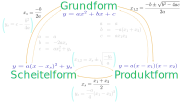
\includegraphics[width=15cm]{allg/funktionen/img/formen/formen.png}
\end{center}

\begin{bemerkung}{}{}
  Das $a$,  ist in allen Formen derselbe Wert und bestimmt die Parabelöffnung.
  \end{bemerkung}
\newpage

\textbf{Grundform aus Scheitelform} (einfaches Ausmultiplizieren). Beispiel:
$$y=2(x-3)^2-4 = 2(x^2-6x+9)-4=2x^2-12x+14$$

\begin{tabular}{rcl}
$a(x-x_S)^2+y_S$ &=& $ax^2-2ax_Sx + (ax_S^2+y_S)$\\
  $a$ &=& $a$ \\
  $b$ &=& $-2ax_S$\\
  $c$ &=& $ax_S^2+y_S$
\end{tabular}


\textbf{Grundform aus Produktform} (einfaches Ausmultiplizieren). Beispiel
$$y=2(x+3)(x-4)=2(x^2 +(3-4)x - 12) = 2x^2-x-24$$

\begin{tabular}{rcl}
  $a(x-x_1)(x-x_2)$ &=& $ax^2 - a(x_1+x_2)x + ax_1x_2$\\
  $a$ &=& $a$ \\
  $b$ &=& $-a(x_1+x_2)$\\
  $c$ &=& $ax_1x_2$
\end{tabular}


\textbf{Nullstellenform (Produktform) aus Grundform}:
Gegeben: $y = ax^2 + bx + c$

Nullstellenform: $y = a(x-x_1)\cdot{}(x-x_2)$ mit

$$x_{1,2} = \frac{-b \pm \sqrt{b^2-4ac}}{2a}$$

\begin{beispiel}{}{}
Gegeben $y = 5x^2 - 5x - 30$. Schreiben Sie dies in der Produktform (=
Nullstellenform):
\platzFuerBerechnungen{3.2}\TRAINER{$y = 5(x-3)(x+2)$\vspace{4.2cm}}
\end{beispiel}
\newpage


\textbf{Scheitelform aus Grundform}:
$$x_S=\frac{-b}{2a}$$

$y_S$ einfach durch Einsetzen von $x_S$ in die Grundform:
$$y_S=c-\frac{b^2}{4a}$$
 
\textbf{Scheitelform aus Produktform}: $x_S$ ist der Mittelwert der beiden
Nullstellen:
$$x_S=\frac{x_1+x_2}{2}$$
Danach $y_S$ einfach durch Einsetzen von $x_S$ in die Produktform:
$$y_S=\frac{-a}{4}(x_1-x_2)^2$$

\textbf{Produktform aus Scheitelform}: Einfachster Weg geht über die Grundform oder abgekürzt:
$$x_{1,2} =x_S \pm \sqrt{\frac{-y_S}{a}}$$


\subsection{Aufgaben}

\TALS{\olatLinkArbeitsblatt{Umrechnen der Formen}{https://olat.bbw.ch/auth/RepositoryEntry/572162090/CourseNode/103176133021102}{1., 2., 3. und 8.}}



\newpage

% Bereits in typ I II und III eingebaut
%\subsection{Parabel aus drei Punkten}
Vorzeigeaufgabe Marthaler Algebra S. 272 Aufg. 3. b) 


\subsection*{Aufgaben}

\AadBMTA{272}{3. a) c)}%% war Marthaler S. 187 Aufg. 676 a) und b)
\GESOAadBMTA{???}{???}

\newpage



%\newpage

%

%%%%%%%%%%%%%%%%%%%%%%%%%%%%%%%%%%%%%%%%%%%%%%%%%%%%%%%%%%%%%%%%
\subsection{Extremwertaufgaben}



\subsubsection{Aus alter Maturprüfung}

\aufgabenFarbe{Gegeben ist die Funktion $f(x) = x\cdot{}(3-\sqrt{x})$,
  $x\in[0;\infty[$.\\
  a) Bestimmen Sie die Nullstellen und das  Extremum der Funktion
  $f$.\\
  b) Im ersten Quadranten, zwischen dem  Graphen und der
  $x$-Achse ist ein  rechtwinkliges Dreieck $ABC$ einbeschrieben.  Der
  rechte Winkel ist in der Ecke $B$.  Punkt $A$ liegt im Ursprung, $B$
  auf der  $x$-Achse und $C$ auf dem Graphen von $f$. Berechnen Sie
  die Koordinaten des  Punktes $C$ so, dass der Flächeninhalt des
  Dreiecks maximal wird.
}%% END aufgabenFarbe

    
\bbwCenterGraphic{8cm}{tals/fct3/img/Maximieren.png}
\TNTeop{
   a) solve$(f(x)=0,x)$ Somit sind die Nullstellen bei 0 und 9\\
     $\text{fmax}(f(x),x)$ liefert $x=4$ ist Maximalstelle (und auch
     Maximalwert ($f(4)=4$)\\
   b) $\text{fmax}(0.5\cdot{}x\cdot{}f(x), x)$ liefert $x = 5.76$ und
   $f(5.76) = 3.456$}%% End TNTeop
\newpage
\subsection*{Aufgaben}
\AadBMTA{311}{49.}
\AadBMTA{321}{17.}

%\newpage

\section{Berührende Graphen}\index{Graphen!berührende}\index{berührende Graphen}

\textbf{Einführungsbeispiel}


Gegeben ist die Parabel $f: y=\frac{1}{4}x^2 -\frac12x +\frac14$ und von einer
Geraden $g$ ist der $y$-Achsenabschnitt $b = -2$ gegeben.

Gesucht ist von der Geraden $g$ die Steigung $a$ so, dass die
Gerade die Parabel tangiert; also genau in einem Punkt berührt.

Wo (in welchem Punkt $B=(x_B|y_B)$) tangiert also die Gerade $g$ die Parabel $f$?

In der folgenden Skizze sind drei mögliche Geraden mit $y$-Achsenabschnitt
$-2$ gezeichnet. Nur eine dieser drei Geraden \textit{tangiert} die Parabel.

\bbwGraph{-4}{4}{-3}{5}{
  \draw[thick,color=blue,variable=\x,domain=-3.5:4] plot ({\x},   {0.25*\x*\x -0.5*\x + 0.25});

  \draw[color=red,variable=\x,domain=-3:5] plot ({\x},{2*\x -2});
  \draw[color=red,variable=\x,domain=-3:5] plot ({\x},{0.5*\x - 2});
  \draw[color=cyan,thick,variable=\x,domain=-3:5] plot ({\x},{1*\x  -2});

  \bbwDot{3, 1}{green}{north}{B}

  %%%\draw[thick,color=blue,variable=\x,domain=-1:5] plot ({\x}, {0.5*\x*\x - 2*\x + 3}); 
  %%\draw[color=red,variable=\x,domain=-1:5] plot ({\x},{0.5*\x + 1});
  %%\draw[color=red,variable=\x,domain=-1:5] plot ({\x},{0.5*\x - 1.5});
  %%\draw[color=cyan,thick,variable=\x,domain=-1:6] plot ({\x},{0.5*\x  -0.125});
  %%\bbwDot{2.5, 1.125}{green}{north}{P}
}
\newpage
\textbf{Lösungsidee}: Der gesuchte Parameter ist $a$, die Steigung der
Geraden.

Nun berechne die Schnittpunkte/den Schnittpunkt mit $$f(x) = g(x).$$

Das $a$ ist gefunden, sobald die Gleichung $f(x)=g(x)$ genau eine
Lösung aufweist; dann also, wenn


\TNT{2}{die Diskriminante dieser Gleichung
verschwindet.}

Den $x$-Wert dieses Berührungspunktes nennen wir $x_B$:


Ansatz:

$$f(x_B) = g(x_B)$$

\TNT{4.4}{
 
\begin{tabular}{rclr}
$\frac14x_s^2-\frac12x_s+\frac14$          & $=$ &  $ax_s-2$ & \\
$\frac14x_s^2+(-\frac12-a)x_s + \frac94$   & $=$ & $0$       & (I)\\
\end{tabular}
\vspace{10mm}
}%% END TNT

Die Diskriminante $D=B^2 - 4AC$ muss gleich 0 sein. 

\TNT{7.2}{
$A = \frac14$, $B = -\frac12-a$ und $C = \frac94$.

  $$D=0=B^2-4AC = (-\frac12-a)^2  - (4\cdot{}A\cdot{}C)$$
  $$0 = (a^2+a+\frac14) - (4\cdot\frac14\cdot{}\frac{+9}4)$$
$$\Longrightarrow 0 = a^2 + a - 2$$
$$\Longrightarrow a_1 = 1 \text{ und  } a_2 = -2$$
\vspace{40mm}
}%% END TNT
\newpage

Für den \textbf{Berührungspunkt} $B=(x_B|y_B)$ müssen wir nun nur doch das gefundene
$a$ in die Gleichung (I) einsetzen.


\TNT{6}{
  $$0 = \frac14x_B^2 + (-\frac12 -a ) + \frac94$$

  $$x_B = x_1 = x_2 = \frac{-B \pm\sqrt{D}}{2A} = \frac{-B \pm
    \sqrt{0}}{2A} = \frac{-B}{2A}$$

  $$x_B = \frac{-B}{2A} = \frac{- (-\frac12 - a)}{\frac24} =
  \frac{\frac12 + a}{\frac12} = (\frac12 + a) : \frac12 = (\frac12+a)
  \cdot{} 2 = 1+2a$$
}



1. Fall: ($a_1=1$):

\TNT{6}{
$B_1: a_1 = 1:$
  $$x_B = 1+2a = 1 + 2\cdot{}(1) = 3$$

Das $y$ finden wir einfach durch Einsetzen von $x$ in den
Funktionsterm der Geradengleichung.

$$y_1 = a_1x_1 - 2 = 1\cdot{}3-2 = 1$$
und somit ist
$$B_1 = (3 | 1)$$
}%% END TNT



2. Fall: ($a_1=-2$):


\TNTeop{
$B_2: a_2 = -2:$
  $$x_B = 1+2a = 1 + 2\cdot{}(-2) = 1-4=-3$$


$$y_2 = a_2x_2+b = -2\cdot{}3-2 = 4$$
und somit ist
$$B_2 = (-3 | 4)$$

}%% END TNT
\newpage




\begin{rezept}{Berührende Graphen}{}

  Bei Berührungsaufgaben mit Parabeln hilft i.\,d.\,R. das folgende
  Vorgehen:

  \begin{enumerate}
  \item Funktionsterme Gleichsetzen: $$f(x) = g(x)$$
  \item In Grundform bringen: $$f(x) - g(x) = 0  \hspace{40mm}
    (I)$$
  \item Diskriminante $D = 0 $ setzen, um den Parameterwert zu
    bestimmen.
  \item Gleichung $(I)$ auflösen mit dem Wissen $D=0$.
    $$x_B=x_1=x_2= \frac{-B}{2A}$$

  \item Gefundenen Parameter in $x_B=\frac{-B}{2A}$ einsetzen, um $x$
    des Berührungspunktes zu bestimmen.
  \item Das $y_B$ des Berührungspunktes ermitteln, indem wir $x_B$ in
    $f$ oder $g$ einsetzen.
    \end{enumerate}
\end{rezept}


\TRAINER{(Je nach Zeit wäre 699. a) noch eine Vorzeigeaufgabe.)}

\subsection{Aufgaben}
\TRAINER{Achtung, dass nicht das Gleichungssystem bereits
  nach dem Gleichsetzen der Graphen aufgestellt wird. Erst nach dem
  Null-Setzen der Diskriminante erhalten wir eine gültige Gleichung
  für das Gleichungssystem.}
%%\TALSAadBMTA{190}{698., 702., 703., 705.}
\TALSAadBMTA{277}{30. a), 36. a), 40. a) c), 42. a), 43. a), 44. a)}
\newpage


\subsection{Grenzwerte und Steigungsfunktion (Optional)}

Wie macht das ein CAS, dass es den tiefsten bzw. den höchsten Punkt
einer Funktion bestimmen kann? Hier ein Erklärungsversuch am Beispiel
der quadratischen Funktion.
Betrachten wir die allgemeine quadratische Funktion $$p: y=ax^2 + bx +
c$$
Mit dem selben $a$ und dem selben $b$ kann ich eine Gerade $s$
definieren, die ich die (Tangenten-)\textbf{Steigungsfunktion}\footnote{Diese
  Steigungsfunktion wird in der Mathematik die
  \textbf{Ableitung}\index{Ableitung} genannt. Genau genommen handelt
  es sich nicht um die Steigung der Parabel, sondern um die Steigung
  einer im Punkt $P=(X_P|f(x_P))$ angelegter Tangente.} nenne:
$$s: y= 2ax+b$$
\newpage


Diese Steigungsfunktion $s$ gibt in jedem Punkt $x$ die Steigung einer
Tangente an die Parabel $p$ an.

\begin{beispiel}{Parabel}{}
  Gegeben ist die Parabel $$p: y=2.5x^2 - 3x + 6.5\text{.}$$

  Wo (für welches $x$) hat diese Parabel
  ihren Tiefpunkt? \TRAINER{Scheitelpunkt:}

  $$x_B =   \LoesungsRaumLen{8cm}{\frac{-b}{2a} = \frac{-(-3)}{2\cdot{}2.5} = 0.6}$$

  Dies ist gleichzeitig die Nullstelle der
  Steigungsfunktion:

  $$s: y= \LoesungsRaumLen{3cm}{2\cdot{}2.5x - 3}$$

  Nullstelle von $s$:

  $$x_0 = \LoesungsRaumLen{7cm}{\frac{3}{2\cdot{}2.5} = 0.6}$$

  Wir können damit aber auch die Steigung in einem ganz anderen Punkt
  \zB für $x=10$ berechnen. Die Parabel $p$ hat an der Stelle $x=10$
  die Tangentensteigung, die durch die Steigungsfunktion im Punkt $10$
  ermittelt wird:

  $$s(10) = \LoesungsRaumLen{40mm}{2\cdot{}10\cdot{2.5} - 3 = 47}$$
  
\end{beispiel}
\newpage

\begin{beispiel}{Gerade gesucht}{}
Gegeben ist die Parabel $$p: y=4x^2 -6x + 3\text{.}$$ Gesucht ist die Gerade
$g: y=ax+b$, sodass die Gerade die Parabel bei $x=7$ berührt.

\begin{enumerate}
\item Die Steigungsfunktion $s$ lautet: $$s:
  y=\LoesungsRaumLen{5cm}{2\cdot{}4x - 6}$$
  
\item Für $x=7$ hat die Steigungsfunktion den Wert \LoesungsRaumLen{1cm}{50}, und somit hat
  die Parabel bei $x=7$ die Steigung \LoesungsRaumLen{1cm}{50}.

  
\item Um den Berührungspunkt $B$ zu finden, setzen wir 7 diesen in $p$
  ein
  $$p(7)= \LoesungsRaumLen{5cm}{4\cdot{}49-6\cdot{}7+3 = 157}$$
  und somit ist
  $$B=(\LoesungsRaum{7}|\LoesungsRaum{157})$$
  
\item Die gesuchte Gerade $g: y=ax+b$ hat also auch die Steigung \LoesungsRaum{50}
  und verläuft durch den Berührungspunkt $B=(\LoesungsRaumLen{9mm}{7}|\LoesungsRaumLen{11mm}{157})$. Also
  $$\LoesungsRaumLen{7cm}{157=50\cdot{}7+b}$$

  Somit ist das gesuchte
  $$b = \LoesungsRaumLen{55mm}{157-50\cdot{}7=-193}$$
  
  und die gesuchte Funktionsgleichung der Geraden lautet: $$y = \LoesungsRaumLen{22mm}{50x-193}$$
  \end{enumerate}
\end{beispiel}

\TRAINER{Idee: Auf mm-Papier eine Funktion $y=\frac1{27}x^3-\frac19
  x^2 - \frac89 x$ vorgeben.

Auftrag: Legen Sie in 5 Punkten eine Tangente an die Funktion und
bestimmen Sie deren Steigung.
Tragen Sie die Steigung in ein neues Koordinatensystem ein: $x$-Achse
= $x$ Wert, $y$-Achse = Steigung der Funktion.
$$f' : y = \frac19 (x-1)^2 - 1 $$
}%%
\newpage

\subsubsection{Beweis der Formel der (Tangenten-)Steigungsfunktion}

Betrachten wir auf auf der $x$-Achse zwei benachbarte Punkte $x$ und
$x+\Delta$. Die Funktionswerte lauten $f(x)$ und $f(x+\Delta)$. Die
\textbf{Steigung} kann nun für eine Gerade bestimmt werden durch:

\bbwCenterGraphic{7cm}{tals/fct3/img/Steigungsfunktion.jpg}

$$\frac{f(x+\Delta) - f(x)}{\Delta}$$

Dies gilt für eine Parabel $p: y=ax^2+bx+c$ näherungsweise auch:
$$\frac{f(x+\Delta)-f(x)}{\Delta} = \frac{(a(x+\Delta)^2 + b(x+\Delta)
  + c) - (ax^2 + bx +c)}{\Delta}=2ax+a\Delta+b$$

Wenn wir nun das $\Delta$ gegen Null gehen lassen, also immer kleinere
Werte einsetzen, so verschwindet der Term $a\cdot{}\Delta$ fast und unsere
Formel stimmt annähernd --- jedoch präzise genug, um dies als Beweis
gelten zu lassen.

Ein anderer Beweis wäre die Tangente effektiv einzusetzen und diese so
zu wählen, dass es genau einen Schnittpunkt gibt, was wieder darauf
zurückführt, dass die Diskriminante = Null gesetzt werden muss. Dann
sind wir exakt, aber der Beweis ist ungleich aufwändiger.
\newpage


\newpage



%% Trigonometrie I%
%%%%%%%%%%%%%%%55
%% Funktionen II TALS Metapackage
\part{Funktionen II}\index{Funktionen!II|textbf}
\renewcommand{\bbwPartID}{FCT2}
%%
%% 2019 07 04 Ph. G. Freimann
%%

\section{Quadratische Funktionen}\index{Funktionen!quadratische}
\sectuntertitel{Geraden im Lande der Parabeln wird dringend angeraten, einen
  Integrationskurs zu besuchen.}
%%%%%%%%%%%%%%%%%%%%%%%%%%%%%%%%%%%%%%%%%%%%%%%%%%%%%%%%%%%%%%%%%%%%%%%%%%%%%%%%%

%%\bbwCenterGraphic{8cm}{tals/fct2/img/lugano2018.jpg}
%%\textit{Bildlegende: Parabeln in Lugano (2018)}
\bbwCenterGraphic{175mm}{tals/fct2/img/paris2022.jpg}
\textit{Bildlegende: Parabeln in den Gärten von Versailles (2022)}

\subsection*{Lernziele}

\begin{itemize}
\item Definition
\item Formen: Scheitel-, Produkt-, Normalform
\item Graphische Darstellung
\item Translationen und Spiegelungen
\end{itemize}

\TadBMTA{260}{15}
%%\TALS{(\cite{frommenwiler17alg} S.183 (Kap. 3.4))}
%%\GESO{(\cite{marthaler21alg}       S.260 (Kap. 15))}

Einstieg: Bilder von Heimgartner/Hunziker.


\textbf{Einstiegsaufgabe: } \aufgabenFarbe{Lösen Sie Aufgaben 1. und 2.
  von Seite 272: Welche der angegebenen Funktionen sind quadratisch?}

\newpage

\subsection{Parabel}\index{Parabel}\index{Normalparabel}

Zeichnen Sie die Funktionen $f: y=x^2$ (= Normalparabel), $y=\frac{1}{3}x^2$

und $y=-0.25\cdot{}x^2$  ins Koordinatensystem:

\bbwGraph{-3}{3}{-3}{7}{
  \TRAINER{\bbwFuncC{\x * \x}{-2.5:2.5}{green}
    \bbwFuncC{-0.25*\x * \x}{-3:3}{green}
    \bbwFuncC{\x * \x / 3}{-3:3}{green}
  }
}


\newpage

\subsection{Grundform}\index{Grundform!quadratische Funktion}\index{Quadratische Funktion!Grundform}
Die Funktion $f(x): x \mapsto y = ax^2 + bx +c$ ist eine
quadratische Funktion in Grundform\index{Grundform!quadratische Funktion}.

Spielen Sie mit \TALS{dem TI-nSpire oder mit} \texttt{geogebra.org} an den Parametern $a$, $b$ und $c$ der Funktionsgleichung $y = a\cdot{}x^2 + b\cdot{} x + c$ herum. Was bewirkt der Parameter

$a$: \LoesungsRaumLang{Parabelöffnung: $|a|$ klein: Breite (weite) Öffnung / $|a|$ groß: Enge, schmale Öffnung. $a < 0$: Parabel ist nach unten geöffnet. $a > 0$: Parabel ist nach oben geöffnet.}

$b$: \LoesungsRaumLang{«Parabelsteigung»\footnote{Mit «Parabelsteigung» ist hier die Steigung der entsprechenden Tangente gemeint.} im Punkt $A(0|c)$}

$c$: \LoesungsRaumLang{$y$-Achsenabschnitt. Damit wird eine Verschiebung der Parabel entlang der $y$-Achse erreicht.}

Versuchen Sie eine Parabel mit Scheitelpunkt $(1|1)$ zu finden\TRAINER{(Lösung: $b=-2a$ und $a+b+c=1$.)}.

\subsection*{Aufgaben}
%%\TALSAadBMTA{184ff}{660. a) c) f), 662. a) b) c) und e)}
\AadBMTA{273}{5., 6., 7., 8. und 9.}
\newpage

\subsection{Vier charakteristische Punkte}
Zeichnen Sie die Funktion
$$p: y = x^2 - 4x + \frac{7}{4}$$

\bbwGraph{-3}{6}{-3}{2}{
\TRAINER{\bbwFunc{\x*\x - 4*\x + 1.75}{-0.2:4}}
}%% end BBW Graph

Wo befinden sich die charakteristischen Punkte?

\TNT{2.4}{\vspace{24mm}}


Die charakteristischen Punkte sind:
\begin{itemize}
\item Schnittpunkt mit $y$-Achse = (\LoesungsRaum{0} | \LoesungsRaum{1.75})
\item Nullstellen: $N_1=(\LoesungsRaum{0.5}| \LoesungsRaum{0}), N_2=( \LoesungsRaum{3.5}|\LoesungsRaum{0})$
\item Scheitelpunkt: $S=(\LoesungsRaum{2}|\LoesungsRaum{-2.25})$
\end{itemize}
 
Wie berechnen sich nun diese Punkte?
\newpage
\subsubsection{Parabelöffnung}
Eigentlich ist die Parabelöffnung kein charakteristischer
Punkt. Dennoch kann man eine $x$-Einheit vom Scheitelpunkt entfernt,
das $a$ der Grundform ($y=ax^2+bx+c$) direkt ablesen. Gehen wir bei
der Normalparabel ($a=1$) vom
Scheitelpunkt um eine Einheit nach rechts, so muss die Parabel um eine
$y$-Einheit nach oben anwachsen.

\TNT{10}{
Parabel durch Scheitelpunkt $P=(-3|1)$ und durch $(-2|2)$ =
verschobene Normalparbel zeichnen.

Parabel mit Scheitelpunkt $P=(2|2)$ durch $(3|0.5)$ zeichnen. Das $a$
ist somit sofort $a=-1.5$ abzulesen.
}

\subsubsection{$y$-Achsenabschnitt}
Genau wie bei der linearen Funktion, gilt für den $y$-Achsenabschnitt,
dass die $x$-Koordinate dieses Punktes Null ist.
$$y = x^2 -4x + 1.75$$
wird mit $x=0$ zu
$y = 1.75$.

Der $y$-Achsenabschnitt ist somit immer das $c$ aus $y = ax^2 + bx +
c$.

\newpage

\subsubsection{Nullstellen}
Wie bei den linearen Funktionen sind auch hier die
Nullstellen die Schnittpunkte mit der $x$-Achse. Dies bedeutet für die
Nullstellen $N(x_0 | y_0)$, dass die $y$-Koordinate = 0 ist. Es gilt
also

$$0 = x^2 - 4 x + \frac{7}{4} $$

Dies ist eine quadratische Gleichung mit den Lösungen:

$$x_{1,2} = \frac{-b \pm \sqrt{b^2-4ac}}{2a}$$ 

\noTRAINER{\platzFuerBerechnungen{2.4}}
\TRAINER{$x_{1} = 0.5; x_{2}=3.5$ (Mitternachtsformel)
  \vspace{3cm}}

\begin{bemerkung}{}{}
  Die Nullstellen der quadratischen Funktion entsprechen den Lösungen
  der zugehörigen quadratischen Funktion (mit $y=0$). Daher gilt
  auch hier: 


  \begin{tabular}{c|p{8cm}}
    Diskriminante $D=b^2-4ac$ > 0 & Es gibt zwei Nullstellen. \\
    \hline\\
    Diskriminante $D=b^2-4ac$ = 0 & Es gibt eine Nullstelle, denn der Scheitelpunkt liegt auf der $x$-Achse.\\
    \hline\\
    Diskriminante $D=b^2-4ac$ < 0 & Es gibt keine Nullstellen, denn die Parabel schneidet die $x$-Achse nicht.\\
  \end{tabular}
  
 \ifisALLINONE{Zum Begriff \textbf{Diskriminante}:  \totalref{diskriminante}}\fi{} 
\end{bemerkung}

\subsection*{Aufgaben}
\AadBMTA{277ff}{28. a) c) }

\newpage



\subsubsection{Scheitelpunkt}\index{Scheitelpunkt}
Der Tief- bzw. Hochpunkt einer Parabel wird \textbf{Scheitelpunkt}
genannt.

Wir berechnen den Scheitelpunkt in zwei Schritten.

\textbf{Erstens:} Wir berechnen den Mittelwert der beiden Nullstellen:
$$x_S := \frac{x_{1} + x_{2}}{2} = \frac{\frac{-b+\sqrt{D}}{2a} + \frac{-b-\sqrt{D}}{2a}}{2} =
\frac{(-b+\sqrt{D}) + (-b-\sqrt{D})}{4a} =\frac{-b}{2a}$$
Dabei ist $D$ die Diskriminante $D=b^2-4ac$.

\platzFuerBerechnungen{2.4}
\TRAINER{$x_S = 2$
\vspace{3cm}}

\textbf{Zweitens:} Wir setzen den gefundenen $x$-Wert
(\LoesungsRaum{2}) in die Funktionsgleichung
ein:
$$y_S = x^2 - 4x + 1.75$$
$$y_S = (\LoesungsRaum{2})^2 - 4\cdot{}(\LoesungsRaum{2}) + 1.75$$

Wir erhalten für den Scheitelpunkt $S$: $S=(x_S | y_S) = (\LoesungsRaum{2} | \LoesungsRaum{-2.25})$.

\begin{gesetz}{Scheitelpunkt}{}
  Der Scheitelpunkt $S$ einer Parabel in der Grundform ($y=ax^2+bx+c$) kann wie folgt
  berechnet werden:

  $$S=\left(\frac{-b}{2a}\middle|\frac{4ac-b^2}{4a}\right)$$

  (Bem.: Der $y$-Wert kann einfach durch Einsetzen des $x$-Wertes in
  die Funktionsgleichnug gefunden werden.)
  \end{gesetz}
  
\subsection*{Aufgaben}
%%\TALSAadBMTA{184ff}{665. a) b) c) 666. a) b) c) e) f) g)}
\AadBMTA{273}{4. (=Aufg. 22. S. 276)}

\newpage

\subsection{Bestimmen der Funktionsgleichung}
\TALS{S. 187 Kap. 3.4.3}

\subsubsection{Referenzaufgaben}

\textbf{TYP I}

Gegeben ist ein Punkt $P$ mit den Koordinaten $(2.3 | -1.5)$. Gesucht ist die reinquadratische Funktion $f: y=a\cdot{}x^2$, welche durch diesen Punkt geht.
Machen Sie vorab eine Skizze.

\bbwGraph{-3}{3}{-2}{1}{
  \TRAINER{\bbwFunc{-0.2836 * \x * \x}{-2.5:2.5}
    \bbwDot{2.3,-1.5}{blue}{west}{P}
  }%% end TRAINER
}%% end BBW Graph

\platzFuerBerechnungen{3.6}

\TRAINER{Idee: Punkt einsetzen: $-1.5 = a\cdot{}(2.3)^2$. Das Auf"|lösen dieser Gleichung liefert $a = \frac{-1.5}{2.3^2}$. Dies liefert $a\approx -0.2836$}

Weitere «TYP 1» Aufgaben wären z. B. $y = 3x^2 - bx + 4$ oder $y=2x^2
-7x + c$ mit anderen Worten alle Parabeln mit genau \textbf{einem}
Parameter, daher «Typ 1».

\newpage



\textbf{TYP II}

Gegeben sind zwei Punkte und wir haben zwei Unbekannte.

\begin{rezept}{}{}
  Gesucht sind $a$ und $c$ aus $y = ax^2 + c$ bei den gegebenen
  Punkten $(7|5)$ und $(2|-4)$.

  Wir lösen dies auch durch Einsetzen der Punkte in die
  Funktionsgleichung und wir erhalten zwei Gleichungen:


  \begin{tabular}{c | r  c  r |}
    (I)  &  $5$ & = & $(7)^2\cdot{} a + c$ \\
    (II) & $-4$ & = &  $(2)^2\cdot{} a + c$ \\
  \end{tabular}

  Durch Subtrahieren der Gleichungen erhalten wir

  \begin{tabular}{c | r  c  r | c}
    (I)  &  $5$ & = & $49\cdot{} a + c$ & \,\\
    (II) & $-4$ & = &  $4\cdot{} a + c$ & $\ominus$\\
  \end{tabular}

  $$9 = 45a$$ und somit
  $$a =\frac{1}{5}.$$

  Dieses $a$ (= $\frac{1}{5}$) setzen wir nun in eine der Gleichungen
  (\zB (I)) ein und erhalten
  $$5=49\cdot{}\frac{1}{5} + c$$
  und nach Auf"|lösen erhalten wir $c=\frac{-24}{5}$.

  Die gesuchte Gleichung lautet also:

  $$y = \frac{1}{5}x^2 - \frac{24}{5}$$
\end{rezept}

Probe durch Einsetzen der $x$-Werte der Punkte in die gefundene Funktionsgleichung:

\TNTeop{}
%%\newpage

\begin{beispiel}{}{}
  Anstelle von $a$ und $c$ können natürlich auch $a$ und $b$ gesucht
  sein. Daher eine zweite Aufgabe.

  Gesucht sind $a$ und $b$ aus $y = ax^2 + bx$ bei den gegebenen

  Punkten $(2|-6)$ und $(-3|5)$.

  Wir lösen dies wiederum durch Einsetzen der Punkte in die
  Funktionsgleichung und wir erhalten die beiden Gleichungen, welche
  wir durch das Additionsverfahren lösen können:

  \begin{tabular}{c | r  c  r | c}
    (I)  &  $-6$ & = & $4a + 2b$ & $\cdot{} 3$ \\
    (II) &   $5$ & = & $9a - 3b$ & $\cdot{} 2$ \\
  \end{tabular}

  somit:
  
  \begin{tabular}{c | r  c  r | c}
    (I')  & $-18$ & = & $12a + 6b$ &\, \\
     \,   & \,    & \,&   \,       & $\oplus$\\
    (II') &  $10$ & = & $18a - 6b$ &\, \\
  \end{tabular}

  Nach Addition der Gleichungen erhalten wir

  $$-8 = 30a$$

  was uns zu $a=\frac{-4}{15}$ bringt.

Dieses $a$ können wir nun wieder in eine der beiden Gleichungen
einsetzen (\zB in (I)):

$$-6=4\cdot{}\frac{-4}{15} + 2b$$

Das Auf"|lösen obiger Gleichung liefert nach Kürzen: $b=\frac{-37}{15}$.

Die gesuchte Funktionsgleichung lautet also

$$y = \frac{-4}{15} x^2 - \frac{37}{15} x.$$

\end{beispiel}

Auch bei «Typ II» kann natürlich jede \textbf{zwei}parametrige quadratische
Funktion herhalten, wie \zB $y=-6cx^2 + bx - c$ durch \textbf{zwei}
gegebene Punkte.
\newpage


\textbf{TYP III}: Gegeben sind hier drei Punkte, wir haben aber auch
drei Unbekannte in $y = ax^2 + bx + c$. Die Punkte sind hier
(1|3), (2|3.5) und (-3|11).

Durch Einsetzen der drei Punkte je in die Funktionsgleichung erhalten
wir drei Gleichungen:

\begin{tabular}{c|r c rcrcr|}
  (I)   & 3   & = & $(1)^2\cdot{}a$  &$+$& $(1)\cdot{}b$  &$+$& c \\ 
  (II)  & 3.5 & = & $(2)^2\cdot{}a$  &$+$& $(2)\cdot{}b$  &$+$& c \\ 
  (III) & 11  & = & $(-3)^2\cdot{}a$ &$+$& $(-3)\cdot{}b$ &$+$& c \\ 
\end{tabular}

Vereinfachen:

\begin{tabular}{c|r c rcrcr|}
  (I)   & 3   & = & $a$  &$+$& $b$  &$+$& c \\ 
  (II)  & 3.5 & = & $4a$ &$+$& $2b$ &$+$& c \\ 
  (III) & 11  & = & $9a$ &$-$& $3b$ &$+$& c \\ 
\end{tabular}

Nun finden wir $a$, indem wir zunächst $c$ durch Subtraktion
eliminieren:

\begin{tabular}{l|r c rcr|}
  (IV) = (II) -   (I) & 0.5  & = & $3a$ &$+$& $b$ \\ 
  (V)  = (III) - (II) & 7.5  & = & $5a$ &$-$& $5b$ \\ 
\end{tabular}

Multiplizieren wir nun die Gleichung (IV) mit 5, so erhalten wir

\begin{tabular}{r|r c rcr|}
  5$\cdot{}$(IV)  & 2.5  & = & $15a$ &$+$& $5b$ \\ 
  (V)             & 7.5  & = & $5a$  &$-$& $5b$ \\ 
\end{tabular}

Durch Addition der beiden Gleichungen (IV) und (V) erhalten wir

$10 = 20a$ oder $a = \frac{1}{2}$.

Um $b$ zu finden, setzen wir $a = \frac{1}{2}$ in (V) ein: $7.5 =
5\cdot{}\frac{1}{2} - 5b$.

Auf"|lösen nach $b$ ergibt $b = -1$.

Zu guter Letzt setzen wir $a = \frac{1}{2}$ und $b=-1$ in die
Gleichung (I) ein, um noch $c$ zu erhalten:

$$3 = a + b + c = \frac{1}{2} - 1 + c$$

Somit ist $c=3.5$ und die Funktionsgleichung lautet:

$$y = \frac{1}{2}x^2 - x + 3.5$$


\TALS{\subsection*{Aufgaben}}
%%\TALSAadBMTA{187ff}{676. a) c), 682., 684.}
\AadBMTA{272}{3. a) c), 20. a) c), 21., 22., 24. a), 25. b)}
\newpage


\subsection{Computer Algebra Systeme (CAS)}\index{CAS}
Das eben gezeigte Beispiel wird in der Praxis meist nicht von Hand,
sondern mit einem Computer-Algebra-System, kurz CAS, gelöst:

\paragraph{Aufgabenstellung}
Gegeben sind wieder drei Punkte (1|3), (2|3.5) und (-3|11).
Gesucht ist die Parabel $y = ax^2 + bx + c$, welche durch die drei
Punkte geht.

Dies wird mit dem \tinspire{} wie folgt gelöst:
\begin{itemize}
\item Definiere die Funktionsgleichung mit
  Parametern\footnote{\tinspire Regel: $ax\ne a\cdot{} x$}:\\
  $$f(x) := a\cdot{}x^2 + b\cdot{}x + c$$
\item Definiere das Gleichungssystem:
  $$gls := \left\{ \begin{array}{l}
    f(1) = 3\\
    f(2) = 3.5\\
    f(-3)= 11\\
  \end{array}\right.$$
\item Löse das Gleichungssystem:
  $$solve(gls,\{a, b, c\})$$
\end{itemize}

\subsection*{Aufgaben}
\AadBMTA{272}{3. b) d)}

\newpage

\subsection{Formen der quadratischen Funktion}
\subsubsection{Nullstellenform}\index{Nullstellenform}

Die \textbf{Nullstellenform} wird auch  «faktorisierte Form» oder
«Produktform» genannt.\index{faktorisierte Form}\index{Produktform}

Beachten Sie die folgende quadr. Funktionsgleichung:

$$y = 3.1(x-5)(x+6)$$

Dies ist eine quadratische Funktion in der sogenannten
\textbf{Nullstellenform}, denn die Nullstellen (hier $x_0 = 5$ oder
$x_0 = -6$) können direkt aus der Funktionsgleichung abgelesen werden.
Wenn wir $y=0$ in die Gleichung setzen (Nullstelle),

$$0 = 3.1(x-5)(x+6)$$
so wird die Gleichung genau dann wahr, wenn (mind.) einer der beiden Klammerausdrücke rechts
gleich Null ist. Die Parabelöffnung (hier 3.1) kann dabei beliebig variieren und ist (neben den Nullstellen) der einzige Parameter.

Die Nullstellenform lautet

\begin{gesetz}{}{}

  $$y = a(x-x_1)\cdot{}(x-x_2)$$

  \end{gesetz}

wobei $x_1$ und $x_2$ die Nullstellen der Parabel bezeichnen. 
\newpage


\subsubsection*{Referenzaufgabe zur Nullstellenform}

\noTRAINER{\bbwGraphic{16cm}{tals/fct2/img/BrunnenNullstellenformOhneKoordinatensystem.png}}
\TRAINER{\bbwGraphic{16cm}{tals/fct2/img/BrunnenNullstellenformMitKoordinatensystem.png}}

Ein parabelförmiger Wasserstrahl spritzt ebenerdig aus einem Brunnen und trifft 7m von der Düse entfernt wieder auf dem Boden auf.
Das Wasser steigt also erst gleich hoch an, wie es danach wieder «herunterfällt».
Dabei wird gemessen, dass 1m von der Düse entfernt der Wasserstrahl 84cm über Boden verläuft.
Können Sie aufrecht unter dem Wasserstrahl hindurchgehen?

Tipp: Skizze und  die Parabelgleichung in Nullstellenform aufschreiben. Die Düse ist der Ursprung der Koordinatensystems.\\

\TNT{5.2}{Die Funktionsgleichung lautet $y=a(x-x_1)(x-x2)$.\\
  Mit den Nullstellen $x_1=0$ und $x_2=7$.\\
  Wir setzen den gemessenen Punkt (1|0.84) in die Gleichung ein und erhalten $0.84 = a\cdot{}(1-0)(1-7)$.\\
  Daraus ergibt sich $a=0.84/(-6) = -0.14 $.\\
  Nun setzen wir 3.5 Meter in die Funktionsgleichung $y = -0.14(x-0)(x-7)$ ein: und erhalten $y=-01.4\cdot{}3.5\cdot{}(-3.5) = 1.715m$; das ist die höchste Parabelstelle.}


\subsection*{Aufgaben}%% Nullstellenform
%%\TALSAadBMTA{185}{663, 678., 680.}
\TALSAadBMTA{277}{30. a) b), 31. b)}
\newpage

%%\TRAINER{\, \newpage}
\subsubsection{Scheitelform}\index{Scheitelform!der quadratischen
  Funktion}
Einstieg: Wo hat die Parabel $f: y=3.6(x-4)^2 + 5$ ihren
Scheitelpunkt?

\TNT{4.4}{CAS: bei $x_S = 4$ und $y_S= 5$; völlig irrelevant ist die 3.6.}

Ist eine quadratische Funktion in der Form
\begin{gesetz}{}{}
$$y = a(x-x_S)^2 + y_S$$
\end{gesetz}
gegeben, so sprechen wir von der \textbf{Scheitelform} oder Scheitelpunktsform.
Das liegt daran, dass diese Parabel ihren Scheitelpunkt bei
$(x_S|y_S)$ hat.

Setzen wir für $x$ = $x_S$ in die Funktionsgleichung, so erhalten wir
gerade die $y$-Koordinate des Scheitelpunktes. Je weiter wir uns nun
mit $x$ von $x_S$ wegbewegen, umso größer wird der Term $(x-x_S)^2$
und zwar in egal welcher Richtung wir uns von $x_S$ wegbewegen, die
$y$-Koordinate verhält sich in beiden Fällen symmetrisch.

Prüfen Sie dies mit TI-nSpire oder \texttt{geogebra.org} an der Funktion

$$y = a\cdot{}(x-p)^2 + q$$

Definieren Sie dabei auch den Punkt $S=(p|q)$. Spielen Sie nun mit
$a$, $p$ und $q$. Was bewirken die Änderungen?
\newpage


\subsubsection{Referenzaufgabe Scheitelform}
Von einer Parabel ist der Scheitel $S(2|3)$ gegeben. Ebenfalls ist bekannt, dass die Parabel durch den Punkt $P\left(-\frac{1}{2}\middle|1\right)$ geht.

  Berechnen Sie die Funktionsgleichung in der Grundform $y = ax^2 + bx + c$. Tipp:
  Schreiben Sie die Funktionsgleichung in der Form $y=a(x - x_S)^2 +  y_S$ und setzen anschließend den Punkt $P$ ein.

  \platzFuerBerechnungen{8.0}%%
  \TRAINER{
    Ansatz:
    $$y = a(x-2)^2 + 3$$
    Jetzt $P$ einsetzen:
    $$1 = a(-\frac{1}{2} - 2)^2 + 3 $$
    Nach $a$ auf"|lösen ergibt:
    $$a=-0.32 (=\frac{-2}{2.5^2})$$
    Nun setzen wir $a=-0.32$ in die Funktionsgleichung $y=a(x-2)^2+3$
    ein:
    $$y=-0.32(x-2)^2+3$$
    und quadrieren das Binom, um die geforderte Grundform zu erhalten:
    $$y = -0.32(x^2 - 4x + 4) + 3 = -0.32x^2 + 1.28x + 1.72$$
  }%%end TRAINER%%

  \subsection*{Aufgabe}
  \AadBMTA{277}{29. a) c) e), 32. a), 33.}
%%  \TALSAadBMTA{185}{679. a), 681., 695., 684. a), 700., 694., 686.(*) und  664.}}

\newpage


\subsection{Umrechnungen der Formen}\index{Formen!der quadratischen Funktion}\index{Quadratische Funktion!Formen}

Nochmals die drei Formen im Überblick:


\begin{tabular}{c|l}
  Form & Funktionsgleichung\\
  \hline\\
  Normalform/Grundform & $f: y= ax^2 + bx + c$\\
  \hline\\
  Nullstellenform, faktorisierte Form oder Produktform & $f: y=a(x-x_0)(x-x_1)$\\
  \hline\\
  Scheitelform & $f: y=a(x-x_S)^2+y_S$\\
  \hline%%
\end{tabular}


\subsubsection{Umrechnungen zwischen den Formen}\index{Umrechnungen!quadratische Funktion}\index{Quadratische Funktion!Umrechnungen}

\begin{center}
  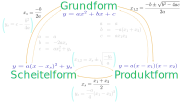
\includegraphics[width=15cm]{allg/funktionen/img/formen/formen.png}
\end{center}

\begin{bemerkung}{}{}
  Das $a$,  ist in allen Formen derselbe Wert und bestimmt die Parabelöffnung.
  \end{bemerkung}
\newpage

\textbf{Grundform aus Scheitelform} (einfaches Ausmultiplizieren). Beispiel:
$$y=2(x-3)^2-4 = 2(x^2-6x+9)-4=2x^2-12x+14$$

\begin{tabular}{rcl}
$a(x-x_S)^2+y_S$ &=& $ax^2-2ax_Sx + (ax_S^2+y_S)$\\
  $a$ &=& $a$ \\
  $b$ &=& $-2ax_S$\\
  $c$ &=& $ax_S^2+y_S$
\end{tabular}


\textbf{Grundform aus Produktform} (einfaches Ausmultiplizieren). Beispiel
$$y=2(x+3)(x-4)=2(x^2 +(3-4)x - 12) = 2x^2-x-24$$

\begin{tabular}{rcl}
  $a(x-x_1)(x-x_2)$ &=& $ax^2 - a(x_1+x_2)x + ax_1x_2$\\
  $a$ &=& $a$ \\
  $b$ &=& $-a(x_1+x_2)$\\
  $c$ &=& $ax_1x_2$
\end{tabular}


\textbf{Nullstellenform (Produktform) aus Grundform}:
Gegeben: $y = ax^2 + bx + c$

Nullstellenform: $y = a(x-x_1)\cdot{}(x-x_2)$ mit

$$x_{1,2} = \frac{-b \pm \sqrt{b^2-4ac}}{2a}$$

\begin{beispiel}{}{}
Gegeben $y = 5x^2 - 5x - 30$. Schreiben Sie dies in der Produktform (=
Nullstellenform):
\platzFuerBerechnungen{3.2}\TRAINER{$y = 5(x-3)(x+2)$\vspace{4.2cm}}
\end{beispiel}
\newpage


\textbf{Scheitelform aus Grundform}:
$$x_S=\frac{-b}{2a}$$

$y_S$ einfach durch Einsetzen von $x_S$ in die Grundform:
$$y_S=c-\frac{b^2}{4a}$$
 
\textbf{Scheitelform aus Produktform}: $x_S$ ist der Mittelwert der beiden
Nullstellen:
$$x_S=\frac{x_1+x_2}{2}$$
Danach $y_S$ einfach durch Einsetzen von $x_S$ in die Produktform:
$$y_S=\frac{-a}{4}(x_1-x_2)^2$$

\textbf{Produktform aus Scheitelform}: Einfachster Weg geht über die Grundform oder abgekürzt:
$$x_{1,2} =x_S \pm \sqrt{\frac{-y_S}{a}}$$


\subsection{Aufgaben}

\TALS{\olatLinkArbeitsblatt{Umrechnen der Formen}{https://olat.bbw.ch/auth/RepositoryEntry/572162090/CourseNode/103176133021102}{1., 2., 3. und 8.}}



\newpage

% Bereits in typ I II und III eingebaut
%\subsection{Parabel aus drei Punkten}
Vorzeigeaufgabe Marthaler Algebra S. 272 Aufg. 3. b) 


\subsection*{Aufgaben}

\AadBMTA{272}{3. a) c)}%% war Marthaler S. 187 Aufg. 676 a) und b)
\GESOAadBMTA{???}{???}

\newpage



%\newpage

%

%%%%%%%%%%%%%%%%%%%%%%%%%%%%%%%%%%%%%%%%%%%%%%%%%%%%%%%%%%%%%%%%
\subsection{Extremwertaufgaben}



\subsubsection{Aus alter Maturprüfung}

\aufgabenFarbe{Gegeben ist die Funktion $f(x) = x\cdot{}(3-\sqrt{x})$,
  $x\in[0;\infty[$.\\
  a) Bestimmen Sie die Nullstellen und das  Extremum der Funktion
  $f$.\\
  b) Im ersten Quadranten, zwischen dem  Graphen und der
  $x$-Achse ist ein  rechtwinkliges Dreieck $ABC$ einbeschrieben.  Der
  rechte Winkel ist in der Ecke $B$.  Punkt $A$ liegt im Ursprung, $B$
  auf der  $x$-Achse und $C$ auf dem Graphen von $f$. Berechnen Sie
  die Koordinaten des  Punktes $C$ so, dass der Flächeninhalt des
  Dreiecks maximal wird.
}%% END aufgabenFarbe

    
\bbwCenterGraphic{8cm}{tals/fct3/img/Maximieren.png}
\TNTeop{
   a) solve$(f(x)=0,x)$ Somit sind die Nullstellen bei 0 und 9\\
     $\text{fmax}(f(x),x)$ liefert $x=4$ ist Maximalstelle (und auch
     Maximalwert ($f(4)=4$)\\
   b) $\text{fmax}(0.5\cdot{}x\cdot{}f(x), x)$ liefert $x = 5.76$ und
   $f(5.76) = 3.456$}%% End TNTeop
\newpage
\subsection*{Aufgaben}
\AadBMTA{311}{49.}
\AadBMTA{321}{17.}

%\newpage

\section{Berührende Graphen}\index{Graphen!berührende}\index{berührende Graphen}

\textbf{Einführungsbeispiel}


Gegeben ist die Parabel $f: y=\frac{1}{4}x^2 -\frac12x +\frac14$ und von einer
Geraden $g$ ist der $y$-Achsenabschnitt $b = -2$ gegeben.

Gesucht ist von der Geraden $g$ die Steigung $a$ so, dass die
Gerade die Parabel tangiert; also genau in einem Punkt berührt.

Wo (in welchem Punkt $B=(x_B|y_B)$) tangiert also die Gerade $g$ die Parabel $f$?

In der folgenden Skizze sind drei mögliche Geraden mit $y$-Achsenabschnitt
$-2$ gezeichnet. Nur eine dieser drei Geraden \textit{tangiert} die Parabel.

\bbwGraph{-4}{4}{-3}{5}{
  \draw[thick,color=blue,variable=\x,domain=-3.5:4] plot ({\x},   {0.25*\x*\x -0.5*\x + 0.25});

  \draw[color=red,variable=\x,domain=-3:5] plot ({\x},{2*\x -2});
  \draw[color=red,variable=\x,domain=-3:5] plot ({\x},{0.5*\x - 2});
  \draw[color=cyan,thick,variable=\x,domain=-3:5] plot ({\x},{1*\x  -2});

  \bbwDot{3, 1}{green}{north}{B}

  %%%\draw[thick,color=blue,variable=\x,domain=-1:5] plot ({\x}, {0.5*\x*\x - 2*\x + 3}); 
  %%\draw[color=red,variable=\x,domain=-1:5] plot ({\x},{0.5*\x + 1});
  %%\draw[color=red,variable=\x,domain=-1:5] plot ({\x},{0.5*\x - 1.5});
  %%\draw[color=cyan,thick,variable=\x,domain=-1:6] plot ({\x},{0.5*\x  -0.125});
  %%\bbwDot{2.5, 1.125}{green}{north}{P}
}
\newpage
\textbf{Lösungsidee}: Der gesuchte Parameter ist $a$, die Steigung der
Geraden.

Nun berechne die Schnittpunkte/den Schnittpunkt mit $$f(x) = g(x).$$

Das $a$ ist gefunden, sobald die Gleichung $f(x)=g(x)$ genau eine
Lösung aufweist; dann also, wenn


\TNT{2}{die Diskriminante dieser Gleichung
verschwindet.}

Den $x$-Wert dieses Berührungspunktes nennen wir $x_B$:


Ansatz:

$$f(x_B) = g(x_B)$$

\TNT{4.4}{
 
\begin{tabular}{rclr}
$\frac14x_s^2-\frac12x_s+\frac14$          & $=$ &  $ax_s-2$ & \\
$\frac14x_s^2+(-\frac12-a)x_s + \frac94$   & $=$ & $0$       & (I)\\
\end{tabular}
\vspace{10mm}
}%% END TNT

Die Diskriminante $D=B^2 - 4AC$ muss gleich 0 sein. 

\TNT{7.2}{
$A = \frac14$, $B = -\frac12-a$ und $C = \frac94$.

  $$D=0=B^2-4AC = (-\frac12-a)^2  - (4\cdot{}A\cdot{}C)$$
  $$0 = (a^2+a+\frac14) - (4\cdot\frac14\cdot{}\frac{+9}4)$$
$$\Longrightarrow 0 = a^2 + a - 2$$
$$\Longrightarrow a_1 = 1 \text{ und  } a_2 = -2$$
\vspace{40mm}
}%% END TNT
\newpage

Für den \textbf{Berührungspunkt} $B=(x_B|y_B)$ müssen wir nun nur doch das gefundene
$a$ in die Gleichung (I) einsetzen.


\TNT{6}{
  $$0 = \frac14x_B^2 + (-\frac12 -a ) + \frac94$$

  $$x_B = x_1 = x_2 = \frac{-B \pm\sqrt{D}}{2A} = \frac{-B \pm
    \sqrt{0}}{2A} = \frac{-B}{2A}$$

  $$x_B = \frac{-B}{2A} = \frac{- (-\frac12 - a)}{\frac24} =
  \frac{\frac12 + a}{\frac12} = (\frac12 + a) : \frac12 = (\frac12+a)
  \cdot{} 2 = 1+2a$$
}



1. Fall: ($a_1=1$):

\TNT{6}{
$B_1: a_1 = 1:$
  $$x_B = 1+2a = 1 + 2\cdot{}(1) = 3$$

Das $y$ finden wir einfach durch Einsetzen von $x$ in den
Funktionsterm der Geradengleichung.

$$y_1 = a_1x_1 - 2 = 1\cdot{}3-2 = 1$$
und somit ist
$$B_1 = (3 | 1)$$
}%% END TNT



2. Fall: ($a_1=-2$):


\TNTeop{
$B_2: a_2 = -2:$
  $$x_B = 1+2a = 1 + 2\cdot{}(-2) = 1-4=-3$$


$$y_2 = a_2x_2+b = -2\cdot{}3-2 = 4$$
und somit ist
$$B_2 = (-3 | 4)$$

}%% END TNT
\newpage




\begin{rezept}{Berührende Graphen}{}

  Bei Berührungsaufgaben mit Parabeln hilft i.\,d.\,R. das folgende
  Vorgehen:

  \begin{enumerate}
  \item Funktionsterme Gleichsetzen: $$f(x) = g(x)$$
  \item In Grundform bringen: $$f(x) - g(x) = 0  \hspace{40mm}
    (I)$$
  \item Diskriminante $D = 0 $ setzen, um den Parameterwert zu
    bestimmen.
  \item Gleichung $(I)$ auflösen mit dem Wissen $D=0$.
    $$x_B=x_1=x_2= \frac{-B}{2A}$$

  \item Gefundenen Parameter in $x_B=\frac{-B}{2A}$ einsetzen, um $x$
    des Berührungspunktes zu bestimmen.
  \item Das $y_B$ des Berührungspunktes ermitteln, indem wir $x_B$ in
    $f$ oder $g$ einsetzen.
    \end{enumerate}
\end{rezept}


\TRAINER{(Je nach Zeit wäre 699. a) noch eine Vorzeigeaufgabe.)}

\subsection{Aufgaben}
\TRAINER{Achtung, dass nicht das Gleichungssystem bereits
  nach dem Gleichsetzen der Graphen aufgestellt wird. Erst nach dem
  Null-Setzen der Diskriminante erhalten wir eine gültige Gleichung
  für das Gleichungssystem.}
%%\TALSAadBMTA{190}{698., 702., 703., 705.}
\TALSAadBMTA{277}{30. a), 36. a), 40. a) c), 42. a), 43. a), 44. a)}
\newpage


\subsection{Grenzwerte und Steigungsfunktion (Optional)}

Wie macht das ein CAS, dass es den tiefsten bzw. den höchsten Punkt
einer Funktion bestimmen kann? Hier ein Erklärungsversuch am Beispiel
der quadratischen Funktion.
Betrachten wir die allgemeine quadratische Funktion $$p: y=ax^2 + bx +
c$$
Mit dem selben $a$ und dem selben $b$ kann ich eine Gerade $s$
definieren, die ich die (Tangenten-)\textbf{Steigungsfunktion}\footnote{Diese
  Steigungsfunktion wird in der Mathematik die
  \textbf{Ableitung}\index{Ableitung} genannt. Genau genommen handelt
  es sich nicht um die Steigung der Parabel, sondern um die Steigung
  einer im Punkt $P=(X_P|f(x_P))$ angelegter Tangente.} nenne:
$$s: y= 2ax+b$$
\newpage


Diese Steigungsfunktion $s$ gibt in jedem Punkt $x$ die Steigung einer
Tangente an die Parabel $p$ an.

\begin{beispiel}{Parabel}{}
  Gegeben ist die Parabel $$p: y=2.5x^2 - 3x + 6.5\text{.}$$

  Wo (für welches $x$) hat diese Parabel
  ihren Tiefpunkt? \TRAINER{Scheitelpunkt:}

  $$x_B =   \LoesungsRaumLen{8cm}{\frac{-b}{2a} = \frac{-(-3)}{2\cdot{}2.5} = 0.6}$$

  Dies ist gleichzeitig die Nullstelle der
  Steigungsfunktion:

  $$s: y= \LoesungsRaumLen{3cm}{2\cdot{}2.5x - 3}$$

  Nullstelle von $s$:

  $$x_0 = \LoesungsRaumLen{7cm}{\frac{3}{2\cdot{}2.5} = 0.6}$$

  Wir können damit aber auch die Steigung in einem ganz anderen Punkt
  \zB für $x=10$ berechnen. Die Parabel $p$ hat an der Stelle $x=10$
  die Tangentensteigung, die durch die Steigungsfunktion im Punkt $10$
  ermittelt wird:

  $$s(10) = \LoesungsRaumLen{40mm}{2\cdot{}10\cdot{2.5} - 3 = 47}$$
  
\end{beispiel}
\newpage

\begin{beispiel}{Gerade gesucht}{}
Gegeben ist die Parabel $$p: y=4x^2 -6x + 3\text{.}$$ Gesucht ist die Gerade
$g: y=ax+b$, sodass die Gerade die Parabel bei $x=7$ berührt.

\begin{enumerate}
\item Die Steigungsfunktion $s$ lautet: $$s:
  y=\LoesungsRaumLen{5cm}{2\cdot{}4x - 6}$$
  
\item Für $x=7$ hat die Steigungsfunktion den Wert \LoesungsRaumLen{1cm}{50}, und somit hat
  die Parabel bei $x=7$ die Steigung \LoesungsRaumLen{1cm}{50}.

  
\item Um den Berührungspunkt $B$ zu finden, setzen wir 7 diesen in $p$
  ein
  $$p(7)= \LoesungsRaumLen{5cm}{4\cdot{}49-6\cdot{}7+3 = 157}$$
  und somit ist
  $$B=(\LoesungsRaum{7}|\LoesungsRaum{157})$$
  
\item Die gesuchte Gerade $g: y=ax+b$ hat also auch die Steigung \LoesungsRaum{50}
  und verläuft durch den Berührungspunkt $B=(\LoesungsRaumLen{9mm}{7}|\LoesungsRaumLen{11mm}{157})$. Also
  $$\LoesungsRaumLen{7cm}{157=50\cdot{}7+b}$$

  Somit ist das gesuchte
  $$b = \LoesungsRaumLen{55mm}{157-50\cdot{}7=-193}$$
  
  und die gesuchte Funktionsgleichung der Geraden lautet: $$y = \LoesungsRaumLen{22mm}{50x-193}$$
  \end{enumerate}
\end{beispiel}

\TRAINER{Idee: Auf mm-Papier eine Funktion $y=\frac1{27}x^3-\frac19
  x^2 - \frac89 x$ vorgeben.

Auftrag: Legen Sie in 5 Punkten eine Tangente an die Funktion und
bestimmen Sie deren Steigung.
Tragen Sie die Steigung in ein neues Koordinatensystem ein: $x$-Achse
= $x$ Wert, $y$-Achse = Steigung der Funktion.
$$f' : y = \frac19 (x-1)^2 - 1 $$
}%%
\newpage

\subsubsection{Beweis der Formel der (Tangenten-)Steigungsfunktion}

Betrachten wir auf auf der $x$-Achse zwei benachbarte Punkte $x$ und
$x+\Delta$. Die Funktionswerte lauten $f(x)$ und $f(x+\Delta)$. Die
\textbf{Steigung} kann nun für eine Gerade bestimmt werden durch:

\bbwCenterGraphic{7cm}{tals/fct3/img/Steigungsfunktion.jpg}

$$\frac{f(x+\Delta) - f(x)}{\Delta}$$

Dies gilt für eine Parabel $p: y=ax^2+bx+c$ näherungsweise auch:
$$\frac{f(x+\Delta)-f(x)}{\Delta} = \frac{(a(x+\Delta)^2 + b(x+\Delta)
  + c) - (ax^2 + bx +c)}{\Delta}=2ax+a\Delta+b$$

Wenn wir nun das $\Delta$ gegen Null gehen lassen, also immer kleinere
Werte einsetzen, so verschwindet der Term $a\cdot{}\Delta$ fast und unsere
Formel stimmt annähernd --- jedoch präzise genug, um dies als Beweis
gelten zu lassen.

Ein anderer Beweis wäre die Tangente effektiv einzusetzen und diese so
zu wählen, dass es genau einen Schnittpunkt gibt, was wieder darauf
zurückführt, dass die Diskriminante = Null gesetzt werden muss. Dann
sind wir exakt, aber der Beweis ist ungleich aufwändiger.
\newpage


\newpage



%% Trigonometrie I%
%%%%%%%%%%%%%%%55
%% Funktionen II TALS Metapackage
\part{Funktionen II}\index{Funktionen!II|textbf}
\renewcommand{\bbwPartID}{FCT2}
%%
%% 2019 07 04 Ph. G. Freimann
%%

\section{Quadratische Funktionen}\index{Funktionen!quadratische}
\sectuntertitel{Geraden im Lande der Parabeln wird dringend angeraten, einen
  Integrationskurs zu besuchen.}
%%%%%%%%%%%%%%%%%%%%%%%%%%%%%%%%%%%%%%%%%%%%%%%%%%%%%%%%%%%%%%%%%%%%%%%%%%%%%%%%%

%%\bbwCenterGraphic{8cm}{tals/fct2/img/lugano2018.jpg}
%%\textit{Bildlegende: Parabeln in Lugano (2018)}
\bbwCenterGraphic{175mm}{tals/fct2/img/paris2022.jpg}
\textit{Bildlegende: Parabeln in den Gärten von Versailles (2022)}

\subsection*{Lernziele}

\begin{itemize}
\item Definition
\item Formen: Scheitel-, Produkt-, Normalform
\item Graphische Darstellung
\item Translationen und Spiegelungen
\end{itemize}

\TadBMTA{260}{15}
%%\TALS{(\cite{frommenwiler17alg} S.183 (Kap. 3.4))}
%%\GESO{(\cite{marthaler21alg}       S.260 (Kap. 15))}

Einstieg: Bilder von Heimgartner/Hunziker.


\textbf{Einstiegsaufgabe: } \aufgabenFarbe{Lösen Sie Aufgaben 1. und 2.
  von Seite 272: Welche der angegebenen Funktionen sind quadratisch?}

\newpage

\subsection{Parabel}\index{Parabel}\index{Normalparabel}

Zeichnen Sie die Funktionen $f: y=x^2$ (= Normalparabel), $y=\frac{1}{3}x^2$

und $y=-0.25\cdot{}x^2$  ins Koordinatensystem:

\bbwGraph{-3}{3}{-3}{7}{
  \TRAINER{\bbwFuncC{\x * \x}{-2.5:2.5}{green}
    \bbwFuncC{-0.25*\x * \x}{-3:3}{green}
    \bbwFuncC{\x * \x / 3}{-3:3}{green}
  }
}


\newpage

\subsection{Grundform}\index{Grundform!quadratische Funktion}\index{Quadratische Funktion!Grundform}
Die Funktion $f(x): x \mapsto y = ax^2 + bx +c$ ist eine
quadratische Funktion in Grundform\index{Grundform!quadratische Funktion}.

Spielen Sie mit \TALS{dem TI-nSpire oder mit} \texttt{geogebra.org} an den Parametern $a$, $b$ und $c$ der Funktionsgleichung $y = a\cdot{}x^2 + b\cdot{} x + c$ herum. Was bewirkt der Parameter

$a$: \LoesungsRaumLang{Parabelöffnung: $|a|$ klein: Breite (weite) Öffnung / $|a|$ groß: Enge, schmale Öffnung. $a < 0$: Parabel ist nach unten geöffnet. $a > 0$: Parabel ist nach oben geöffnet.}

$b$: \LoesungsRaumLang{«Parabelsteigung»\footnote{Mit «Parabelsteigung» ist hier die Steigung der entsprechenden Tangente gemeint.} im Punkt $A(0|c)$}

$c$: \LoesungsRaumLang{$y$-Achsenabschnitt. Damit wird eine Verschiebung der Parabel entlang der $y$-Achse erreicht.}

Versuchen Sie eine Parabel mit Scheitelpunkt $(1|1)$ zu finden\TRAINER{(Lösung: $b=-2a$ und $a+b+c=1$.)}.

\subsection*{Aufgaben}
%%\TALSAadBMTA{184ff}{660. a) c) f), 662. a) b) c) und e)}
\AadBMTA{273}{5., 6., 7., 8. und 9.}
\newpage

\subsection{Vier charakteristische Punkte}
Zeichnen Sie die Funktion
$$p: y = x^2 - 4x + \frac{7}{4}$$

\bbwGraph{-3}{6}{-3}{2}{
\TRAINER{\bbwFunc{\x*\x - 4*\x + 1.75}{-0.2:4}}
}%% end BBW Graph

Wo befinden sich die charakteristischen Punkte?

\TNT{2.4}{\vspace{24mm}}


Die charakteristischen Punkte sind:
\begin{itemize}
\item Schnittpunkt mit $y$-Achse = (\LoesungsRaum{0} | \LoesungsRaum{1.75})
\item Nullstellen: $N_1=(\LoesungsRaum{0.5}| \LoesungsRaum{0}), N_2=( \LoesungsRaum{3.5}|\LoesungsRaum{0})$
\item Scheitelpunkt: $S=(\LoesungsRaum{2}|\LoesungsRaum{-2.25})$
\end{itemize}
 
Wie berechnen sich nun diese Punkte?
\newpage
\subsubsection{Parabelöffnung}
Eigentlich ist die Parabelöffnung kein charakteristischer
Punkt. Dennoch kann man eine $x$-Einheit vom Scheitelpunkt entfernt,
das $a$ der Grundform ($y=ax^2+bx+c$) direkt ablesen. Gehen wir bei
der Normalparabel ($a=1$) vom
Scheitelpunkt um eine Einheit nach rechts, so muss die Parabel um eine
$y$-Einheit nach oben anwachsen.

\TNT{10}{
Parabel durch Scheitelpunkt $P=(-3|1)$ und durch $(-2|2)$ =
verschobene Normalparbel zeichnen.

Parabel mit Scheitelpunkt $P=(2|2)$ durch $(3|0.5)$ zeichnen. Das $a$
ist somit sofort $a=-1.5$ abzulesen.
}

\subsubsection{$y$-Achsenabschnitt}
Genau wie bei der linearen Funktion, gilt für den $y$-Achsenabschnitt,
dass die $x$-Koordinate dieses Punktes Null ist.
$$y = x^2 -4x + 1.75$$
wird mit $x=0$ zu
$y = 1.75$.

Der $y$-Achsenabschnitt ist somit immer das $c$ aus $y = ax^2 + bx +
c$.

\newpage

\subsubsection{Nullstellen}
Wie bei den linearen Funktionen sind auch hier die
Nullstellen die Schnittpunkte mit der $x$-Achse. Dies bedeutet für die
Nullstellen $N(x_0 | y_0)$, dass die $y$-Koordinate = 0 ist. Es gilt
also

$$0 = x^2 - 4 x + \frac{7}{4} $$

Dies ist eine quadratische Gleichung mit den Lösungen:

$$x_{1,2} = \frac{-b \pm \sqrt{b^2-4ac}}{2a}$$ 

\noTRAINER{\platzFuerBerechnungen{2.4}}
\TRAINER{$x_{1} = 0.5; x_{2}=3.5$ (Mitternachtsformel)
  \vspace{3cm}}

\begin{bemerkung}{}{}
  Die Nullstellen der quadratischen Funktion entsprechen den Lösungen
  der zugehörigen quadratischen Funktion (mit $y=0$). Daher gilt
  auch hier: 


  \begin{tabular}{c|p{8cm}}
    Diskriminante $D=b^2-4ac$ > 0 & Es gibt zwei Nullstellen. \\
    \hline\\
    Diskriminante $D=b^2-4ac$ = 0 & Es gibt eine Nullstelle, denn der Scheitelpunkt liegt auf der $x$-Achse.\\
    \hline\\
    Diskriminante $D=b^2-4ac$ < 0 & Es gibt keine Nullstellen, denn die Parabel schneidet die $x$-Achse nicht.\\
  \end{tabular}
  
 \ifisALLINONE{Zum Begriff \textbf{Diskriminante}:  \totalref{diskriminante}}\fi{} 
\end{bemerkung}

\subsection*{Aufgaben}
\AadBMTA{277ff}{28. a) c) }

\newpage



\subsubsection{Scheitelpunkt}\index{Scheitelpunkt}
Der Tief- bzw. Hochpunkt einer Parabel wird \textbf{Scheitelpunkt}
genannt.

Wir berechnen den Scheitelpunkt in zwei Schritten.

\textbf{Erstens:} Wir berechnen den Mittelwert der beiden Nullstellen:
$$x_S := \frac{x_{1} + x_{2}}{2} = \frac{\frac{-b+\sqrt{D}}{2a} + \frac{-b-\sqrt{D}}{2a}}{2} =
\frac{(-b+\sqrt{D}) + (-b-\sqrt{D})}{4a} =\frac{-b}{2a}$$
Dabei ist $D$ die Diskriminante $D=b^2-4ac$.

\platzFuerBerechnungen{2.4}
\TRAINER{$x_S = 2$
\vspace{3cm}}

\textbf{Zweitens:} Wir setzen den gefundenen $x$-Wert
(\LoesungsRaum{2}) in die Funktionsgleichung
ein:
$$y_S = x^2 - 4x + 1.75$$
$$y_S = (\LoesungsRaum{2})^2 - 4\cdot{}(\LoesungsRaum{2}) + 1.75$$

Wir erhalten für den Scheitelpunkt $S$: $S=(x_S | y_S) = (\LoesungsRaum{2} | \LoesungsRaum{-2.25})$.

\begin{gesetz}{Scheitelpunkt}{}
  Der Scheitelpunkt $S$ einer Parabel in der Grundform ($y=ax^2+bx+c$) kann wie folgt
  berechnet werden:

  $$S=\left(\frac{-b}{2a}\middle|\frac{4ac-b^2}{4a}\right)$$

  (Bem.: Der $y$-Wert kann einfach durch Einsetzen des $x$-Wertes in
  die Funktionsgleichnug gefunden werden.)
  \end{gesetz}
  
\subsection*{Aufgaben}
%%\TALSAadBMTA{184ff}{665. a) b) c) 666. a) b) c) e) f) g)}
\AadBMTA{273}{4. (=Aufg. 22. S. 276)}

\newpage

\subsection{Bestimmen der Funktionsgleichung}
\TALS{S. 187 Kap. 3.4.3}

\subsubsection{Referenzaufgaben}

\textbf{TYP I}

Gegeben ist ein Punkt $P$ mit den Koordinaten $(2.3 | -1.5)$. Gesucht ist die reinquadratische Funktion $f: y=a\cdot{}x^2$, welche durch diesen Punkt geht.
Machen Sie vorab eine Skizze.

\bbwGraph{-3}{3}{-2}{1}{
  \TRAINER{\bbwFunc{-0.2836 * \x * \x}{-2.5:2.5}
    \bbwDot{2.3,-1.5}{blue}{west}{P}
  }%% end TRAINER
}%% end BBW Graph

\platzFuerBerechnungen{3.6}

\TRAINER{Idee: Punkt einsetzen: $-1.5 = a\cdot{}(2.3)^2$. Das Auf"|lösen dieser Gleichung liefert $a = \frac{-1.5}{2.3^2}$. Dies liefert $a\approx -0.2836$}

Weitere «TYP 1» Aufgaben wären z. B. $y = 3x^2 - bx + 4$ oder $y=2x^2
-7x + c$ mit anderen Worten alle Parabeln mit genau \textbf{einem}
Parameter, daher «Typ 1».

\newpage



\textbf{TYP II}

Gegeben sind zwei Punkte und wir haben zwei Unbekannte.

\begin{rezept}{}{}
  Gesucht sind $a$ und $c$ aus $y = ax^2 + c$ bei den gegebenen
  Punkten $(7|5)$ und $(2|-4)$.

  Wir lösen dies auch durch Einsetzen der Punkte in die
  Funktionsgleichung und wir erhalten zwei Gleichungen:


  \begin{tabular}{c | r  c  r |}
    (I)  &  $5$ & = & $(7)^2\cdot{} a + c$ \\
    (II) & $-4$ & = &  $(2)^2\cdot{} a + c$ \\
  \end{tabular}

  Durch Subtrahieren der Gleichungen erhalten wir

  \begin{tabular}{c | r  c  r | c}
    (I)  &  $5$ & = & $49\cdot{} a + c$ & \,\\
    (II) & $-4$ & = &  $4\cdot{} a + c$ & $\ominus$\\
  \end{tabular}

  $$9 = 45a$$ und somit
  $$a =\frac{1}{5}.$$

  Dieses $a$ (= $\frac{1}{5}$) setzen wir nun in eine der Gleichungen
  (\zB (I)) ein und erhalten
  $$5=49\cdot{}\frac{1}{5} + c$$
  und nach Auf"|lösen erhalten wir $c=\frac{-24}{5}$.

  Die gesuchte Gleichung lautet also:

  $$y = \frac{1}{5}x^2 - \frac{24}{5}$$
\end{rezept}

Probe durch Einsetzen der $x$-Werte der Punkte in die gefundene Funktionsgleichung:

\TNTeop{}
%%\newpage

\begin{beispiel}{}{}
  Anstelle von $a$ und $c$ können natürlich auch $a$ und $b$ gesucht
  sein. Daher eine zweite Aufgabe.

  Gesucht sind $a$ und $b$ aus $y = ax^2 + bx$ bei den gegebenen

  Punkten $(2|-6)$ und $(-3|5)$.

  Wir lösen dies wiederum durch Einsetzen der Punkte in die
  Funktionsgleichung und wir erhalten die beiden Gleichungen, welche
  wir durch das Additionsverfahren lösen können:

  \begin{tabular}{c | r  c  r | c}
    (I)  &  $-6$ & = & $4a + 2b$ & $\cdot{} 3$ \\
    (II) &   $5$ & = & $9a - 3b$ & $\cdot{} 2$ \\
  \end{tabular}

  somit:
  
  \begin{tabular}{c | r  c  r | c}
    (I')  & $-18$ & = & $12a + 6b$ &\, \\
     \,   & \,    & \,&   \,       & $\oplus$\\
    (II') &  $10$ & = & $18a - 6b$ &\, \\
  \end{tabular}

  Nach Addition der Gleichungen erhalten wir

  $$-8 = 30a$$

  was uns zu $a=\frac{-4}{15}$ bringt.

Dieses $a$ können wir nun wieder in eine der beiden Gleichungen
einsetzen (\zB in (I)):

$$-6=4\cdot{}\frac{-4}{15} + 2b$$

Das Auf"|lösen obiger Gleichung liefert nach Kürzen: $b=\frac{-37}{15}$.

Die gesuchte Funktionsgleichung lautet also

$$y = \frac{-4}{15} x^2 - \frac{37}{15} x.$$

\end{beispiel}

Auch bei «Typ II» kann natürlich jede \textbf{zwei}parametrige quadratische
Funktion herhalten, wie \zB $y=-6cx^2 + bx - c$ durch \textbf{zwei}
gegebene Punkte.
\newpage


\textbf{TYP III}: Gegeben sind hier drei Punkte, wir haben aber auch
drei Unbekannte in $y = ax^2 + bx + c$. Die Punkte sind hier
(1|3), (2|3.5) und (-3|11).

Durch Einsetzen der drei Punkte je in die Funktionsgleichung erhalten
wir drei Gleichungen:

\begin{tabular}{c|r c rcrcr|}
  (I)   & 3   & = & $(1)^2\cdot{}a$  &$+$& $(1)\cdot{}b$  &$+$& c \\ 
  (II)  & 3.5 & = & $(2)^2\cdot{}a$  &$+$& $(2)\cdot{}b$  &$+$& c \\ 
  (III) & 11  & = & $(-3)^2\cdot{}a$ &$+$& $(-3)\cdot{}b$ &$+$& c \\ 
\end{tabular}

Vereinfachen:

\begin{tabular}{c|r c rcrcr|}
  (I)   & 3   & = & $a$  &$+$& $b$  &$+$& c \\ 
  (II)  & 3.5 & = & $4a$ &$+$& $2b$ &$+$& c \\ 
  (III) & 11  & = & $9a$ &$-$& $3b$ &$+$& c \\ 
\end{tabular}

Nun finden wir $a$, indem wir zunächst $c$ durch Subtraktion
eliminieren:

\begin{tabular}{l|r c rcr|}
  (IV) = (II) -   (I) & 0.5  & = & $3a$ &$+$& $b$ \\ 
  (V)  = (III) - (II) & 7.5  & = & $5a$ &$-$& $5b$ \\ 
\end{tabular}

Multiplizieren wir nun die Gleichung (IV) mit 5, so erhalten wir

\begin{tabular}{r|r c rcr|}
  5$\cdot{}$(IV)  & 2.5  & = & $15a$ &$+$& $5b$ \\ 
  (V)             & 7.5  & = & $5a$  &$-$& $5b$ \\ 
\end{tabular}

Durch Addition der beiden Gleichungen (IV) und (V) erhalten wir

$10 = 20a$ oder $a = \frac{1}{2}$.

Um $b$ zu finden, setzen wir $a = \frac{1}{2}$ in (V) ein: $7.5 =
5\cdot{}\frac{1}{2} - 5b$.

Auf"|lösen nach $b$ ergibt $b = -1$.

Zu guter Letzt setzen wir $a = \frac{1}{2}$ und $b=-1$ in die
Gleichung (I) ein, um noch $c$ zu erhalten:

$$3 = a + b + c = \frac{1}{2} - 1 + c$$

Somit ist $c=3.5$ und die Funktionsgleichung lautet:

$$y = \frac{1}{2}x^2 - x + 3.5$$


\TALS{\subsection*{Aufgaben}}
%%\TALSAadBMTA{187ff}{676. a) c), 682., 684.}
\AadBMTA{272}{3. a) c), 20. a) c), 21., 22., 24. a), 25. b)}
\newpage


\subsection{Computer Algebra Systeme (CAS)}\index{CAS}
Das eben gezeigte Beispiel wird in der Praxis meist nicht von Hand,
sondern mit einem Computer-Algebra-System, kurz CAS, gelöst:

\paragraph{Aufgabenstellung}
Gegeben sind wieder drei Punkte (1|3), (2|3.5) und (-3|11).
Gesucht ist die Parabel $y = ax^2 + bx + c$, welche durch die drei
Punkte geht.

Dies wird mit dem \tinspire{} wie folgt gelöst:
\begin{itemize}
\item Definiere die Funktionsgleichung mit
  Parametern\footnote{\tinspire Regel: $ax\ne a\cdot{} x$}:\\
  $$f(x) := a\cdot{}x^2 + b\cdot{}x + c$$
\item Definiere das Gleichungssystem:
  $$gls := \left\{ \begin{array}{l}
    f(1) = 3\\
    f(2) = 3.5\\
    f(-3)= 11\\
  \end{array}\right.$$
\item Löse das Gleichungssystem:
  $$solve(gls,\{a, b, c\})$$
\end{itemize}

\subsection*{Aufgaben}
\AadBMTA{272}{3. b) d)}

\newpage

\subsection{Formen der quadratischen Funktion}
\subsubsection{Nullstellenform}\index{Nullstellenform}

Die \textbf{Nullstellenform} wird auch  «faktorisierte Form» oder
«Produktform» genannt.\index{faktorisierte Form}\index{Produktform}

Beachten Sie die folgende quadr. Funktionsgleichung:

$$y = 3.1(x-5)(x+6)$$

Dies ist eine quadratische Funktion in der sogenannten
\textbf{Nullstellenform}, denn die Nullstellen (hier $x_0 = 5$ oder
$x_0 = -6$) können direkt aus der Funktionsgleichung abgelesen werden.
Wenn wir $y=0$ in die Gleichung setzen (Nullstelle),

$$0 = 3.1(x-5)(x+6)$$
so wird die Gleichung genau dann wahr, wenn (mind.) einer der beiden Klammerausdrücke rechts
gleich Null ist. Die Parabelöffnung (hier 3.1) kann dabei beliebig variieren und ist (neben den Nullstellen) der einzige Parameter.

Die Nullstellenform lautet

\begin{gesetz}{}{}

  $$y = a(x-x_1)\cdot{}(x-x_2)$$

  \end{gesetz}

wobei $x_1$ und $x_2$ die Nullstellen der Parabel bezeichnen. 
\newpage


\subsubsection*{Referenzaufgabe zur Nullstellenform}

\noTRAINER{\bbwGraphic{16cm}{tals/fct2/img/BrunnenNullstellenformOhneKoordinatensystem.png}}
\TRAINER{\bbwGraphic{16cm}{tals/fct2/img/BrunnenNullstellenformMitKoordinatensystem.png}}

Ein parabelförmiger Wasserstrahl spritzt ebenerdig aus einem Brunnen und trifft 7m von der Düse entfernt wieder auf dem Boden auf.
Das Wasser steigt also erst gleich hoch an, wie es danach wieder «herunterfällt».
Dabei wird gemessen, dass 1m von der Düse entfernt der Wasserstrahl 84cm über Boden verläuft.
Können Sie aufrecht unter dem Wasserstrahl hindurchgehen?

Tipp: Skizze und  die Parabelgleichung in Nullstellenform aufschreiben. Die Düse ist der Ursprung der Koordinatensystems.\\

\TNT{5.2}{Die Funktionsgleichung lautet $y=a(x-x_1)(x-x2)$.\\
  Mit den Nullstellen $x_1=0$ und $x_2=7$.\\
  Wir setzen den gemessenen Punkt (1|0.84) in die Gleichung ein und erhalten $0.84 = a\cdot{}(1-0)(1-7)$.\\
  Daraus ergibt sich $a=0.84/(-6) = -0.14 $.\\
  Nun setzen wir 3.5 Meter in die Funktionsgleichung $y = -0.14(x-0)(x-7)$ ein: und erhalten $y=-01.4\cdot{}3.5\cdot{}(-3.5) = 1.715m$; das ist die höchste Parabelstelle.}


\subsection*{Aufgaben}%% Nullstellenform
%%\TALSAadBMTA{185}{663, 678., 680.}
\TALSAadBMTA{277}{30. a) b), 31. b)}
\newpage

%%\TRAINER{\, \newpage}
\subsubsection{Scheitelform}\index{Scheitelform!der quadratischen
  Funktion}
Einstieg: Wo hat die Parabel $f: y=3.6(x-4)^2 + 5$ ihren
Scheitelpunkt?

\TNT{4.4}{CAS: bei $x_S = 4$ und $y_S= 5$; völlig irrelevant ist die 3.6.}

Ist eine quadratische Funktion in der Form
\begin{gesetz}{}{}
$$y = a(x-x_S)^2 + y_S$$
\end{gesetz}
gegeben, so sprechen wir von der \textbf{Scheitelform} oder Scheitelpunktsform.
Das liegt daran, dass diese Parabel ihren Scheitelpunkt bei
$(x_S|y_S)$ hat.

Setzen wir für $x$ = $x_S$ in die Funktionsgleichung, so erhalten wir
gerade die $y$-Koordinate des Scheitelpunktes. Je weiter wir uns nun
mit $x$ von $x_S$ wegbewegen, umso größer wird der Term $(x-x_S)^2$
und zwar in egal welcher Richtung wir uns von $x_S$ wegbewegen, die
$y$-Koordinate verhält sich in beiden Fällen symmetrisch.

Prüfen Sie dies mit TI-nSpire oder \texttt{geogebra.org} an der Funktion

$$y = a\cdot{}(x-p)^2 + q$$

Definieren Sie dabei auch den Punkt $S=(p|q)$. Spielen Sie nun mit
$a$, $p$ und $q$. Was bewirken die Änderungen?
\newpage


\subsubsection{Referenzaufgabe Scheitelform}
Von einer Parabel ist der Scheitel $S(2|3)$ gegeben. Ebenfalls ist bekannt, dass die Parabel durch den Punkt $P\left(-\frac{1}{2}\middle|1\right)$ geht.

  Berechnen Sie die Funktionsgleichung in der Grundform $y = ax^2 + bx + c$. Tipp:
  Schreiben Sie die Funktionsgleichung in der Form $y=a(x - x_S)^2 +  y_S$ und setzen anschließend den Punkt $P$ ein.

  \platzFuerBerechnungen{8.0}%%
  \TRAINER{
    Ansatz:
    $$y = a(x-2)^2 + 3$$
    Jetzt $P$ einsetzen:
    $$1 = a(-\frac{1}{2} - 2)^2 + 3 $$
    Nach $a$ auf"|lösen ergibt:
    $$a=-0.32 (=\frac{-2}{2.5^2})$$
    Nun setzen wir $a=-0.32$ in die Funktionsgleichung $y=a(x-2)^2+3$
    ein:
    $$y=-0.32(x-2)^2+3$$
    und quadrieren das Binom, um die geforderte Grundform zu erhalten:
    $$y = -0.32(x^2 - 4x + 4) + 3 = -0.32x^2 + 1.28x + 1.72$$
  }%%end TRAINER%%

  \subsection*{Aufgabe}
  \AadBMTA{277}{29. a) c) e), 32. a), 33.}
%%  \TALSAadBMTA{185}{679. a), 681., 695., 684. a), 700., 694., 686.(*) und  664.}}

\newpage


\subsection{Umrechnungen der Formen}\index{Formen!der quadratischen Funktion}\index{Quadratische Funktion!Formen}

Nochmals die drei Formen im Überblick:


\begin{tabular}{c|l}
  Form & Funktionsgleichung\\
  \hline\\
  Normalform/Grundform & $f: y= ax^2 + bx + c$\\
  \hline\\
  Nullstellenform, faktorisierte Form oder Produktform & $f: y=a(x-x_0)(x-x_1)$\\
  \hline\\
  Scheitelform & $f: y=a(x-x_S)^2+y_S$\\
  \hline%%
\end{tabular}


\subsubsection{Umrechnungen zwischen den Formen}\index{Umrechnungen!quadratische Funktion}\index{Quadratische Funktion!Umrechnungen}

\begin{center}
  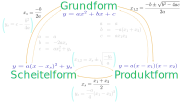
\includegraphics[width=15cm]{allg/funktionen/img/formen/formen.png}
\end{center}

\begin{bemerkung}{}{}
  Das $a$,  ist in allen Formen derselbe Wert und bestimmt die Parabelöffnung.
  \end{bemerkung}
\newpage

\textbf{Grundform aus Scheitelform} (einfaches Ausmultiplizieren). Beispiel:
$$y=2(x-3)^2-4 = 2(x^2-6x+9)-4=2x^2-12x+14$$

\begin{tabular}{rcl}
$a(x-x_S)^2+y_S$ &=& $ax^2-2ax_Sx + (ax_S^2+y_S)$\\
  $a$ &=& $a$ \\
  $b$ &=& $-2ax_S$\\
  $c$ &=& $ax_S^2+y_S$
\end{tabular}


\textbf{Grundform aus Produktform} (einfaches Ausmultiplizieren). Beispiel
$$y=2(x+3)(x-4)=2(x^2 +(3-4)x - 12) = 2x^2-x-24$$

\begin{tabular}{rcl}
  $a(x-x_1)(x-x_2)$ &=& $ax^2 - a(x_1+x_2)x + ax_1x_2$\\
  $a$ &=& $a$ \\
  $b$ &=& $-a(x_1+x_2)$\\
  $c$ &=& $ax_1x_2$
\end{tabular}


\textbf{Nullstellenform (Produktform) aus Grundform}:
Gegeben: $y = ax^2 + bx + c$

Nullstellenform: $y = a(x-x_1)\cdot{}(x-x_2)$ mit

$$x_{1,2} = \frac{-b \pm \sqrt{b^2-4ac}}{2a}$$

\begin{beispiel}{}{}
Gegeben $y = 5x^2 - 5x - 30$. Schreiben Sie dies in der Produktform (=
Nullstellenform):
\platzFuerBerechnungen{3.2}\TRAINER{$y = 5(x-3)(x+2)$\vspace{4.2cm}}
\end{beispiel}
\newpage


\textbf{Scheitelform aus Grundform}:
$$x_S=\frac{-b}{2a}$$

$y_S$ einfach durch Einsetzen von $x_S$ in die Grundform:
$$y_S=c-\frac{b^2}{4a}$$
 
\textbf{Scheitelform aus Produktform}: $x_S$ ist der Mittelwert der beiden
Nullstellen:
$$x_S=\frac{x_1+x_2}{2}$$
Danach $y_S$ einfach durch Einsetzen von $x_S$ in die Produktform:
$$y_S=\frac{-a}{4}(x_1-x_2)^2$$

\textbf{Produktform aus Scheitelform}: Einfachster Weg geht über die Grundform oder abgekürzt:
$$x_{1,2} =x_S \pm \sqrt{\frac{-y_S}{a}}$$


\subsection{Aufgaben}

\TALS{\olatLinkArbeitsblatt{Umrechnen der Formen}{https://olat.bbw.ch/auth/RepositoryEntry/572162090/CourseNode/103176133021102}{1., 2., 3. und 8.}}



\newpage

% Bereits in typ I II und III eingebaut
%\subsection{Parabel aus drei Punkten}
Vorzeigeaufgabe Marthaler Algebra S. 272 Aufg. 3. b) 


\subsection*{Aufgaben}

\AadBMTA{272}{3. a) c)}%% war Marthaler S. 187 Aufg. 676 a) und b)
\GESOAadBMTA{???}{???}

\newpage



%\newpage

%

%%%%%%%%%%%%%%%%%%%%%%%%%%%%%%%%%%%%%%%%%%%%%%%%%%%%%%%%%%%%%%%%
\subsection{Extremwertaufgaben}



\subsubsection{Aus alter Maturprüfung}

\aufgabenFarbe{Gegeben ist die Funktion $f(x) = x\cdot{}(3-\sqrt{x})$,
  $x\in[0;\infty[$.\\
  a) Bestimmen Sie die Nullstellen und das  Extremum der Funktion
  $f$.\\
  b) Im ersten Quadranten, zwischen dem  Graphen und der
  $x$-Achse ist ein  rechtwinkliges Dreieck $ABC$ einbeschrieben.  Der
  rechte Winkel ist in der Ecke $B$.  Punkt $A$ liegt im Ursprung, $B$
  auf der  $x$-Achse und $C$ auf dem Graphen von $f$. Berechnen Sie
  die Koordinaten des  Punktes $C$ so, dass der Flächeninhalt des
  Dreiecks maximal wird.
}%% END aufgabenFarbe

    
\bbwCenterGraphic{8cm}{tals/fct3/img/Maximieren.png}
\TNTeop{
   a) solve$(f(x)=0,x)$ Somit sind die Nullstellen bei 0 und 9\\
     $\text{fmax}(f(x),x)$ liefert $x=4$ ist Maximalstelle (und auch
     Maximalwert ($f(4)=4$)\\
   b) $\text{fmax}(0.5\cdot{}x\cdot{}f(x), x)$ liefert $x = 5.76$ und
   $f(5.76) = 3.456$}%% End TNTeop
\newpage
\subsection*{Aufgaben}
\AadBMTA{311}{49.}
\AadBMTA{321}{17.}

%\newpage

\section{Berührende Graphen}\index{Graphen!berührende}\index{berührende Graphen}

\textbf{Einführungsbeispiel}


Gegeben ist die Parabel $f: y=\frac{1}{4}x^2 -\frac12x +\frac14$ und von einer
Geraden $g$ ist der $y$-Achsenabschnitt $b = -2$ gegeben.

Gesucht ist von der Geraden $g$ die Steigung $a$ so, dass die
Gerade die Parabel tangiert; also genau in einem Punkt berührt.

Wo (in welchem Punkt $B=(x_B|y_B)$) tangiert also die Gerade $g$ die Parabel $f$?

In der folgenden Skizze sind drei mögliche Geraden mit $y$-Achsenabschnitt
$-2$ gezeichnet. Nur eine dieser drei Geraden \textit{tangiert} die Parabel.

\bbwGraph{-4}{4}{-3}{5}{
  \draw[thick,color=blue,variable=\x,domain=-3.5:4] plot ({\x},   {0.25*\x*\x -0.5*\x + 0.25});

  \draw[color=red,variable=\x,domain=-3:5] plot ({\x},{2*\x -2});
  \draw[color=red,variable=\x,domain=-3:5] plot ({\x},{0.5*\x - 2});
  \draw[color=cyan,thick,variable=\x,domain=-3:5] plot ({\x},{1*\x  -2});

  \bbwDot{3, 1}{green}{north}{B}

  %%%\draw[thick,color=blue,variable=\x,domain=-1:5] plot ({\x}, {0.5*\x*\x - 2*\x + 3}); 
  %%\draw[color=red,variable=\x,domain=-1:5] plot ({\x},{0.5*\x + 1});
  %%\draw[color=red,variable=\x,domain=-1:5] plot ({\x},{0.5*\x - 1.5});
  %%\draw[color=cyan,thick,variable=\x,domain=-1:6] plot ({\x},{0.5*\x  -0.125});
  %%\bbwDot{2.5, 1.125}{green}{north}{P}
}
\newpage
\textbf{Lösungsidee}: Der gesuchte Parameter ist $a$, die Steigung der
Geraden.

Nun berechne die Schnittpunkte/den Schnittpunkt mit $$f(x) = g(x).$$

Das $a$ ist gefunden, sobald die Gleichung $f(x)=g(x)$ genau eine
Lösung aufweist; dann also, wenn


\TNT{2}{die Diskriminante dieser Gleichung
verschwindet.}

Den $x$-Wert dieses Berührungspunktes nennen wir $x_B$:


Ansatz:

$$f(x_B) = g(x_B)$$

\TNT{4.4}{
 
\begin{tabular}{rclr}
$\frac14x_s^2-\frac12x_s+\frac14$          & $=$ &  $ax_s-2$ & \\
$\frac14x_s^2+(-\frac12-a)x_s + \frac94$   & $=$ & $0$       & (I)\\
\end{tabular}
\vspace{10mm}
}%% END TNT

Die Diskriminante $D=B^2 - 4AC$ muss gleich 0 sein. 

\TNT{7.2}{
$A = \frac14$, $B = -\frac12-a$ und $C = \frac94$.

  $$D=0=B^2-4AC = (-\frac12-a)^2  - (4\cdot{}A\cdot{}C)$$
  $$0 = (a^2+a+\frac14) - (4\cdot\frac14\cdot{}\frac{+9}4)$$
$$\Longrightarrow 0 = a^2 + a - 2$$
$$\Longrightarrow a_1 = 1 \text{ und  } a_2 = -2$$
\vspace{40mm}
}%% END TNT
\newpage

Für den \textbf{Berührungspunkt} $B=(x_B|y_B)$ müssen wir nun nur doch das gefundene
$a$ in die Gleichung (I) einsetzen.


\TNT{6}{
  $$0 = \frac14x_B^2 + (-\frac12 -a ) + \frac94$$

  $$x_B = x_1 = x_2 = \frac{-B \pm\sqrt{D}}{2A} = \frac{-B \pm
    \sqrt{0}}{2A} = \frac{-B}{2A}$$

  $$x_B = \frac{-B}{2A} = \frac{- (-\frac12 - a)}{\frac24} =
  \frac{\frac12 + a}{\frac12} = (\frac12 + a) : \frac12 = (\frac12+a)
  \cdot{} 2 = 1+2a$$
}



1. Fall: ($a_1=1$):

\TNT{6}{
$B_1: a_1 = 1:$
  $$x_B = 1+2a = 1 + 2\cdot{}(1) = 3$$

Das $y$ finden wir einfach durch Einsetzen von $x$ in den
Funktionsterm der Geradengleichung.

$$y_1 = a_1x_1 - 2 = 1\cdot{}3-2 = 1$$
und somit ist
$$B_1 = (3 | 1)$$
}%% END TNT



2. Fall: ($a_1=-2$):


\TNTeop{
$B_2: a_2 = -2:$
  $$x_B = 1+2a = 1 + 2\cdot{}(-2) = 1-4=-3$$


$$y_2 = a_2x_2+b = -2\cdot{}3-2 = 4$$
und somit ist
$$B_2 = (-3 | 4)$$

}%% END TNT
\newpage




\begin{rezept}{Berührende Graphen}{}

  Bei Berührungsaufgaben mit Parabeln hilft i.\,d.\,R. das folgende
  Vorgehen:

  \begin{enumerate}
  \item Funktionsterme Gleichsetzen: $$f(x) = g(x)$$
  \item In Grundform bringen: $$f(x) - g(x) = 0  \hspace{40mm}
    (I)$$
  \item Diskriminante $D = 0 $ setzen, um den Parameterwert zu
    bestimmen.
  \item Gleichung $(I)$ auflösen mit dem Wissen $D=0$.
    $$x_B=x_1=x_2= \frac{-B}{2A}$$

  \item Gefundenen Parameter in $x_B=\frac{-B}{2A}$ einsetzen, um $x$
    des Berührungspunktes zu bestimmen.
  \item Das $y_B$ des Berührungspunktes ermitteln, indem wir $x_B$ in
    $f$ oder $g$ einsetzen.
    \end{enumerate}
\end{rezept}


\TRAINER{(Je nach Zeit wäre 699. a) noch eine Vorzeigeaufgabe.)}

\subsection{Aufgaben}
\TRAINER{Achtung, dass nicht das Gleichungssystem bereits
  nach dem Gleichsetzen der Graphen aufgestellt wird. Erst nach dem
  Null-Setzen der Diskriminante erhalten wir eine gültige Gleichung
  für das Gleichungssystem.}
%%\TALSAadBMTA{190}{698., 702., 703., 705.}
\TALSAadBMTA{277}{30. a), 36. a), 40. a) c), 42. a), 43. a), 44. a)}
\newpage


\subsection{Grenzwerte und Steigungsfunktion (Optional)}

Wie macht das ein CAS, dass es den tiefsten bzw. den höchsten Punkt
einer Funktion bestimmen kann? Hier ein Erklärungsversuch am Beispiel
der quadratischen Funktion.
Betrachten wir die allgemeine quadratische Funktion $$p: y=ax^2 + bx +
c$$
Mit dem selben $a$ und dem selben $b$ kann ich eine Gerade $s$
definieren, die ich die (Tangenten-)\textbf{Steigungsfunktion}\footnote{Diese
  Steigungsfunktion wird in der Mathematik die
  \textbf{Ableitung}\index{Ableitung} genannt. Genau genommen handelt
  es sich nicht um die Steigung der Parabel, sondern um die Steigung
  einer im Punkt $P=(X_P|f(x_P))$ angelegter Tangente.} nenne:
$$s: y= 2ax+b$$
\newpage


Diese Steigungsfunktion $s$ gibt in jedem Punkt $x$ die Steigung einer
Tangente an die Parabel $p$ an.

\begin{beispiel}{Parabel}{}
  Gegeben ist die Parabel $$p: y=2.5x^2 - 3x + 6.5\text{.}$$

  Wo (für welches $x$) hat diese Parabel
  ihren Tiefpunkt? \TRAINER{Scheitelpunkt:}

  $$x_B =   \LoesungsRaumLen{8cm}{\frac{-b}{2a} = \frac{-(-3)}{2\cdot{}2.5} = 0.6}$$

  Dies ist gleichzeitig die Nullstelle der
  Steigungsfunktion:

  $$s: y= \LoesungsRaumLen{3cm}{2\cdot{}2.5x - 3}$$

  Nullstelle von $s$:

  $$x_0 = \LoesungsRaumLen{7cm}{\frac{3}{2\cdot{}2.5} = 0.6}$$

  Wir können damit aber auch die Steigung in einem ganz anderen Punkt
  \zB für $x=10$ berechnen. Die Parabel $p$ hat an der Stelle $x=10$
  die Tangentensteigung, die durch die Steigungsfunktion im Punkt $10$
  ermittelt wird:

  $$s(10) = \LoesungsRaumLen{40mm}{2\cdot{}10\cdot{2.5} - 3 = 47}$$
  
\end{beispiel}
\newpage

\begin{beispiel}{Gerade gesucht}{}
Gegeben ist die Parabel $$p: y=4x^2 -6x + 3\text{.}$$ Gesucht ist die Gerade
$g: y=ax+b$, sodass die Gerade die Parabel bei $x=7$ berührt.

\begin{enumerate}
\item Die Steigungsfunktion $s$ lautet: $$s:
  y=\LoesungsRaumLen{5cm}{2\cdot{}4x - 6}$$
  
\item Für $x=7$ hat die Steigungsfunktion den Wert \LoesungsRaumLen{1cm}{50}, und somit hat
  die Parabel bei $x=7$ die Steigung \LoesungsRaumLen{1cm}{50}.

  
\item Um den Berührungspunkt $B$ zu finden, setzen wir 7 diesen in $p$
  ein
  $$p(7)= \LoesungsRaumLen{5cm}{4\cdot{}49-6\cdot{}7+3 = 157}$$
  und somit ist
  $$B=(\LoesungsRaum{7}|\LoesungsRaum{157})$$
  
\item Die gesuchte Gerade $g: y=ax+b$ hat also auch die Steigung \LoesungsRaum{50}
  und verläuft durch den Berührungspunkt $B=(\LoesungsRaumLen{9mm}{7}|\LoesungsRaumLen{11mm}{157})$. Also
  $$\LoesungsRaumLen{7cm}{157=50\cdot{}7+b}$$

  Somit ist das gesuchte
  $$b = \LoesungsRaumLen{55mm}{157-50\cdot{}7=-193}$$
  
  und die gesuchte Funktionsgleichung der Geraden lautet: $$y = \LoesungsRaumLen{22mm}{50x-193}$$
  \end{enumerate}
\end{beispiel}

\TRAINER{Idee: Auf mm-Papier eine Funktion $y=\frac1{27}x^3-\frac19
  x^2 - \frac89 x$ vorgeben.

Auftrag: Legen Sie in 5 Punkten eine Tangente an die Funktion und
bestimmen Sie deren Steigung.
Tragen Sie die Steigung in ein neues Koordinatensystem ein: $x$-Achse
= $x$ Wert, $y$-Achse = Steigung der Funktion.
$$f' : y = \frac19 (x-1)^2 - 1 $$
}%%
\newpage

\subsubsection{Beweis der Formel der (Tangenten-)Steigungsfunktion}

Betrachten wir auf auf der $x$-Achse zwei benachbarte Punkte $x$ und
$x+\Delta$. Die Funktionswerte lauten $f(x)$ und $f(x+\Delta)$. Die
\textbf{Steigung} kann nun für eine Gerade bestimmt werden durch:

\bbwCenterGraphic{7cm}{tals/fct3/img/Steigungsfunktion.jpg}

$$\frac{f(x+\Delta) - f(x)}{\Delta}$$

Dies gilt für eine Parabel $p: y=ax^2+bx+c$ näherungsweise auch:
$$\frac{f(x+\Delta)-f(x)}{\Delta} = \frac{(a(x+\Delta)^2 + b(x+\Delta)
  + c) - (ax^2 + bx +c)}{\Delta}=2ax+a\Delta+b$$

Wenn wir nun das $\Delta$ gegen Null gehen lassen, also immer kleinere
Werte einsetzen, so verschwindet der Term $a\cdot{}\Delta$ fast und unsere
Formel stimmt annähernd --- jedoch präzise genug, um dies als Beweis
gelten zu lassen.

Ein anderer Beweis wäre die Tangente effektiv einzusetzen und diese so
zu wählen, dass es genau einen Schnittpunkt gibt, was wieder darauf
zurückführt, dass die Diskriminante = Null gesetzt werden muss. Dann
sind wir exakt, aber der Beweis ist ungleich aufwändiger.
\newpage


\newpage



\scriptEnde{}
